%% NYU PhD thesis format. Created by José Koiller 2007--2008.
%% Updated by Anshul Vikram Pandey with new design guidelines. 2017-2018

%% Use the first of the following lines during production to
%% easily spot "overfull boxes" in the output. Use the second
%% line for the final version.
\documentclass[12pt,draft,letterpaper]{report}
% \documentclass[12pt,letterpaper]{report}
% \documentclass[12pt]{article}

%% Replace the title, name, advisor name, graduation date and dedication below with
%% your own. Graduation months must be January, May or September.
\newcommand{\thesistitle}{USING~VISUAL~ANALYTICS~TO~EXPLAIN
BLACK-BOX~MACHINE~LEARNING}
\newcommand{\thesisauthor}{Josua Walter Hugo Krause}
\newcommand{\thesisadvisor}{Enrico Bertini, Ph.D.}
\newcommand{\graddate}{May 2018} % like January XX, May 20XX, September 20XX

%% If you do not want a dedication, scroll down and comment out
%% the appropriate lines in this file.
\newcommand{\thesisdedication}{To all the Ph.D. pursuing brave souls}

%% The following makes chapters and sections, but not subsections,
%% appear in the TOC (table of contents). Increase to 2 or 3 to
%% make subsections or subsubsections appear, respectively. It seems
%% to be usual to use the "1" setting, however.
\setcounter{tocdepth}{2}

%% Sectional units up to subsubsections are numbered. To number
%% subsections, but not subsubsections, decrease this counter to 2.
\setcounter{secnumdepth}{3}

% Setting a gap between page number and text block


%% Page layout (customized to letter paper and NYU requirements):
\setlength{\oddsidemargin}{.6in}
\setlength{\textwidth}{5.8in}
\setlength{\topmargin}{0.5in}
\setlength{\headheight}{0in}
\setlength{\headsep}{0in}
\setlength{\textheight}{8.3in}
\setlength{\footskip}{.5in}

%% Use the following commands, if desired, during production.
%% Comment them out for final version.
%\usepackage{layout} % defines the \layout command, see below
%\setlength{\hoffset}{-.75in} % creates a large right margin for notes and \showlabels

%% Controls spacing between lines (\doublespacing, \onehalfspacing, etc.):
\usepackage{setspace}

%
%% \usepackage{amsmath}
%% \usepackage{amssymb}
\usepackage{xspace}
\usepackage{algorithmic}
\usepackage{algorithm}
\usepackage{microtype}
% \usepackage{subfigure}
\usepackage{color}
\usepackage{url}
\usepackage{lipsum}
\usepackage{fancyhdr}
% \newfloat{algorithm}{t}{lop}

\pagestyle{fancy}
\fancyhf{}
\renewcommand{\headrulewidth}{0pt}
\fancyhead[L]{}
\fancyhead[R]{}
% \fancyhead[LE]{}
% \fancyhead[RO]{}
% \fancyhead[RE]{}
% \fancyhead[LO]{}
\fancyfoot[C]{}
\rhead{\thepage}

\fancypagestyle{plain}{%
\fancyhf{}
\rhead{\thepage}
}

\setlength{\headheight}{20pt} 

%% Use the line below for official NYU version, which requires
%% double line spacing. For all other uses, this is unnecessary,
%% so the line can be commented out.
\onehalfspacing % requires package setspace, invoked above

%% Each of the following lines defines the \com command, which produces
%% a comment (notes for yourself, for instance) in the output file.
%% Example:    \com{this will appear as a comment in the output}
%% Choose (uncomment) only one of the three forms:
%\newcommand{\com}[1]{[/// {#1} ///]}       % between [/// and ///].
\newcommand{\com}[1]{\marginpar{\tiny #1}} % as (tiny) margin notes
%\newcommand{\com}[1]{}                     % suppress all comments.

%% This inputs your auxiliary file with \usepackage's and \newcommand's:
%% It is assumed that that file is called "definitions.tex".
%%
%% Place here your \usepackage's. Some recommended packages are already included.
%%

% Graphics:
\usepackage[final]{graphicx}
%\usepackage{graphicx} % use this line instead of the above to suppress graphics in draft copies
%\usepackage{graphpap} % \defines the \graphpaper command

% Indent first line of each section:
\usepackage{indentfirst}

% Good AMS stuff:
\usepackage{amsthm} % facilities for theorem-like environments
\usepackage[tbtags]{amsmath} % a lot of good stuff!

% Fonts and symbols:
\usepackage{amsfonts}
\usepackage{amssymb}

\usepackage{xspace}
\usepackage{algorithmic}
\usepackage{algorithm}
\usepackage{microtype}
% \usepackage{subfigure}
\usepackage{color}
% \usepackage{todonotes}
\usepackage{url}
\newfloat{algorithm}{t}{lop}

% Formatting tools:
%\usepackage{relsize} % relative font size selection, provides commands \textsmalle, \textlarger
%\usepackage{xspace} % gentle spacing in macros, such as \newcommand{\acims}{\textsc{acim}s\xspace}

% Page formatting utility:
%\usepackage{geometry}
\usepackage{multirow}

%
\usepackage{listings}


%
\usepackage[numbers,sort]{natbib}

\usepackage[all,cmtip]{xy}

\usepackage{hyperref}
\hypersetup{
    colorlinks=true,
    linkcolor=blue,
    filecolor=blue,
    urlcolor=blue,
    citecolor=blue
}

% additional packages from proposal
% % \renewcommand{\familydefault}{\sfdefault}
% \usepackage[scaled=0.85]{beramono}
\usepackage{wrapfig}
% % \usepackage{caption}
\usepackage{subcaption}
\usepackage{tikz}
% \usepackage{natbib}
% % \usepackage[usenames,dvipsnames]{xcolor}
% % \usepackage{float}
% % \usepackage[rflt]{floatflt}
% \usepackage{hyperref}
% \hypersetup{
%     colorlinks = true,
%     allcolors = {black}
%     % citecolor = {blue},
%     % anchorcolor = {black}
% }

\usepackage{enumitem}
%%%

%%
%% Place here your \newcommand's and \renewcommand's. Some examples already included.
%%
%\newcommand{\acims}{\textsc{acim}s\xspace}
\newcommand{\Mspace}        {{\mathbb M}}
\newcommand{\Rspace}        {{\mathbb R}}
\newcommand{\Cspace}        {{\mathbb C}}

\newcommand{\Mo}        {{\hat M}}
\newcommand{\Ms}        {{\tilde M}}
\newcommand{\Do}          {{\hat D}}
\newcommand{\Ds}        {{\tilde D}}
\newcommand{\doo}          {{\hat d}}
\newcommand{\dss}        {{\tilde d}}
\newcommand{\w}        {{\mathbf w}}

% general
\newcommand{\reffig}[1]{{Figure~\ref{#1}}}
\newcommand{\refchap}[1]{{Chapter~\ref{#1}}}
\newcommand{\refsec}[1]{{Section~\ref{#1}}}
\newcommand{\reftab}[1]{{Table~\ref{#1}}}
\newcommand{\refapp}[1]{{Appendix~\ref{#1}}}
\newcommand{\refeq}[1]{{Equation~\ref{#1}}}
\newcommand{\refalg}[1]{{Algorithm~\ref{#1}}}
\newcommand{\myparagraph}[1]{\noindent \textbf{#1}}
\newcommand{\highlight}[1]{{\color{black}#1}}

\newcommand{\todo}[1]{\textcolor{blue}{[TODO] #1}\PackageWarning{definitions}{[TODO] #1}}
\newcommand{\expand}{\textcolor{green}{[EXPAND]}\PackageWarning{definitions}{EXPAND}}

\newcommand{\eg}{\emph{e.g.}\xspace}
\newcommand{\ie}{\emph{i.e.}\xspace}
\newcommand{\etc}{\emph{etc.}\xspace}
\newcommand{\wrt}{\emph{w.r.t.}\xspace}
\newcommand{\etal}{\emph{et~al.}\xspace}

\newcommand{\figref}[2][]{Figure~\ref{#2}#1\xspace}
\newcommand{\chapref}[1]{Chapter~\ref{#1}\xspace}
\newcommand{\secref}[1]{Section~\ref{#1}\xspace}
\newcommand{\infuse}{\emph{INFUSE}\xspace}

\newcommand{\prospector}{\emph{Prospector}\xspace}

\newcommand{\tabA}{Statistical Summary View\xspace}
\newcommand{\tabB}{Explanation Explorer\xspace}
\newcommand{\tabC}{Item Level Inspector\xspace}

\DeclareMathOperator*{\argmin}{arg\,min}
\DeclareMathOperator*{\argmax}{arg\,max}

% \newcommand{\ainfo}[1]{\phantom{#1}}
\newcommand{\ainfo}[1]{#1}

%%
%% Place here your \newtheorem's:
%%

%% Some examples commented out below. Create your own or use these...
%%%%%%%%%\swapnumbers % this makes the numbers appear before the statement name.
%\theoremstyle{plain}
%\newtheorem{thm}{Theorem}[chapter]
%\newtheorem{prop}[thm]{Proposition}
%\newtheorem{lemma}[thm]{Lemma}
%\newtheorem{cor}[thm]{Corollary}

%\theoremstyle{definition}
%\newtheorem{define}{Definition}[chapter]

%\theoremstyle{remark}
%\newtheorem*{rmk*}{Remark}
%\newtheorem*{rmks*}{Remarks}

%% This defines the "proo" environment, which is the same as proof, but
%% with "Proof:" instead of "Proof.". I prefer the former.
%\newenvironment{proo}{\begin{proof}[Proof:]}{\end{proof}}


%% Cross-referencing utilities. Use one or the other--whichever you prefer--
%% but comment out both lines for final version.
%\usepackage{showlabels}
%\usepackage{showkeys}
% \pagestyle{headings}

\begin{document}
%% Produces a test "layout" page, for "debugging" purposes only.
%% Comment out for final version.
%\layout % requires package layout (see above, on this same file)
%% Sets page numbering to "roman style" i, ii, iii, iv, etc:

%%%%%% Cover page %%%%%%%%%%%
%% Sets page numbering to "roman style" i, ii, iii, iv, etc:
\pagenumbering{roman}
\thispagestyle{empty}
\begin{center}
{\bfseries 
  {\large\thesistitle}
  \vspace{1in}
  
 {\large {\bf DISSERTATION}}\\
  \vspace{.5in}
  
  \begin{doublespace}
  {\large  
  Submitted in Partial Fulfillment of\\
  % \vspace{.1in}
  the Requirements for\\
  % \vspace{.1in}
  the Degree of\\}
  \end{doublespace}
  \vspace{.5in}
  
  {\large DOCTOR OF PHILOSOPHY (Computer Science)}\\
  \vspace{.5in}
  
  at the \\
  \vspace{.2in}
  
  {\large
  NEW YORK UNIVERSITY\\
  \vspace{-0.05in}
  TANDON SCHOOL OF ENGINEERING\\
  }
  \vspace{.2in}
  
  by
  \vspace{.5in}

  {\large\thesisauthor}
  \vspace{.5in}
  % \vfill

  {\large\graddate}
}

\end{center}

\newpage

%%%%%% Title page %%%%%%%%%%%
%
\setcounter{page}{1}
%% No numbering in the title page:
\thispagestyle{empty}
%
\begin{center}
{\bfseries 
  {\large\thesistitle}
  \vspace{.25in}
  
  DISSERTATION\\
  \vspace{.25in}
  
  \begin{doublespace}
  Submitted in Partial Fulfillment of\\
  % \vspace{.1in}
  the Requirements for\\
  % \vspace{.1in}
  the Degree of\\
  \end{doublespace}
  \vspace{.25in}
  
  DOCTOR OF PHILOSOPHY (Computer Science)\\
  \vspace{.25in}
  
  at the \\
  \vspace{.1in}
  
  {\large
  NEW YORK UNIVERSITY\\
  \vspace{-0.05in}
  TANDON SCHOOL OF ENGINEERING\\
  }
  \vspace{.2in}
  
  by
  \vspace{.3in}

  \thesisauthor
  \vspace{.3in}
  % \vfill

  \graddate
}

\end{center}
% \vfill

\vspace{0.2in}

\noindent
\makebox[\textwidth]{\hfill\makebox[2.5in]{Approved: \hfill}}
\vspace{0.1in}

\noindent
\makebox[\textwidth]{\hfill\makebox[2.5in]{\hrulefill}}\\
\makebox[\textwidth]{\hfill\makebox[2.5in]{\hfill Department Head Signature\hfill}}
\vspace{0.05in}

\noindent
\makebox[\textwidth]{\hfill\makebox[2.5in]{\hrulefill}}\\
\makebox[\textwidth]{\hfill\makebox[2.5in]{\hfill Date \hfill}}

\noindent
Copy No.\hspace{33pt} \noindent\rule[-3pt]{2in}{0.4pt}\\
University ID\#:      \noindent\rule[-3pt]{2in}{0.4pt}\\

%\newpage

%%%%%%%%%%%%%% Copyright Page %%%%%%%%%%%%%%%%%

%%%%%%%%%%%%%% Guidance Committee Signature Page %%%%%%%%%%%%%%%%%
Approved by the Guidance Committee:
\singlespacing

\underline{Major}: Computer Science
\vspace{0.7in}

\noindent
\makebox[\textwidth]{\hfill\makebox[3in]{\hrulefill}}\\
\makebox[\textwidth]{\hfill\makebox[3in]{\hfill \textbf{Advisor's Name}\hfill}}
\makebox[\textwidth]{\hfill\makebox[3in]{\hfill Professor of \hfill}}
\makebox[\textwidth]{\hfill\makebox[3in]{\hfill Computer Science and Engineering \hfill}}
\makebox[\textwidth]{\hfill\makebox[3in]{\rule[-4pt]{2in}{1pt}}}\\
\makebox[\textwidth]{\hfill\makebox[3in]{\hfill Date \hfill}}\\
\vspace{0.5in}

\noindent
\makebox[\textwidth]{\hfill\makebox[3in]{\hrulefill}}\\
\makebox[\textwidth]{\hfill\makebox[3in]{\hfill \textbf{Advisor's Name}\hfill}}
\makebox[\textwidth]{\hfill\makebox[3in]{\hfill Professor of \hfill}}
\makebox[\textwidth]{\hfill\makebox[3in]{\hfill Computer Science and Engineering \hfill}}
\makebox[\textwidth]{\hfill\makebox[3in]{\rule[-4pt]{2in}{1pt}}}\\
\makebox[\textwidth]{\hfill\makebox[3in]{\hfill Date \hfill}}\\
\vspace{0.5in}


\noindent
\makebox[\textwidth]{\hfill\makebox[3in]{\hrulefill}}\\
\makebox[\textwidth]{\hfill\makebox[3in]{\hfill \textbf{Advisor's Name}\hfill}}
\makebox[\textwidth]{\hfill\makebox[3in]{\hfill Assistant Professor of \hfill}}
\makebox[\textwidth]{\hfill\makebox[3in]{\hfill Computer Science and Engineering \hfill}}
\makebox[\textwidth]{\hfill\makebox[3in]{\rule[-4pt]{2in}{1pt}}}\\
\makebox[\textwidth]{\hfill\makebox[3in]{\hfill Date \hfill}}\\
\vspace{0.5in}

\noindent
\makebox[\textwidth]{\hfill\makebox[3in]{\hrulefill}}\\
\makebox[\textwidth]{\hfill\makebox[3in]{\hfill \textbf{Advisor's Name}\hfill}}
\makebox[\textwidth]{\hfill\makebox[3in]{\hfill Assistant Professor of XXX\hfill}}
\makebox[\textwidth]{\hfill\makebox[3in]{\hfill Computer Science and Engineering \hfill}}
\makebox[\textwidth]{\hfill\makebox[3in]{\rule[-4pt]{2in}{1pt}}}\\
\makebox[\textwidth]{\hfill\makebox[3in]{\hfill Date \hfill}}\\

\doublespacing

%%%%%%%%%%%%%% Microfilm / Publishing Page %%%%%%%%%%%%%%%%%
\begin{center}
Microfilm or other copies of this dissertation are obtainable from
\vspace{4in}

UMI Dissertation Publishing\\
ProQuest CSA\\
789 E. Eisenhower Parkway\\
P.O. Box 1346\\
Ann Arbor, MI 48106-1346

\end{center}
\newpage

%%%%%%%%%%%%%% Vita %%%%%%%%%%%%%%%%%
\section*{Vita}
\addcontentsline{toc}{section}{Vita}
%!TEX root = thesis.tex

\todo{TODO}
Your vita goes here. This is usually a paragraph or two. Be careful about what you write here. :)

\lipsum[1]
\newpage



%%%%%%%%%%%%%% Ackknowlegment %%%%%%%%%%%%%%%%%
%% Comment out the following lines if you do not want to acknowledge
%% anyone's help...
\section*{Acknowledgements}
\addcontentsline{toc}{section}{Acknowledgements}
%!TEX root = thesis.tex

%% Write your acknowledgements in this file. If you do not want to acknowledge anyone,
%% you can delete this file and comment out the corresponding part in the "thesis.tex"
%% file.
\lipsum[1]

\noindent
\makebox[\textwidth]{\hfill\makebox[3in]{\hfill Your Name\hfill}}
\makebox[\textwidth]{\hfill\makebox[3in]{\hfill\graddate\hfill}}


\newpage

%%%%%%%%%%%%%% Dedication Page %%%%%%%%%%%%%%%%%
%% Comment out the following lines if you do not want to dedicate
%% this to anyone...
\vspace*{\fill}
\begin{center}
  \thesisdedication%\addcontentsline{toc}{section}{Dedication}
\end{center}
\vfill
\newpage


%%%%%%%%%%%%%% Abstract %%%%%%%%%%%%%%%%%
\section*{}
\begin{center}
{\bfseries 
  %{\large\thesistitle}
  \vspace{.25in}  
  {\bf ABSTRACT}\\
  \vspace{.25in}
  {\bf \thesistitle}\\  
  \vspace{.25in}
  {\bf by}\\  
  \vspace{.5in}
  {\bf \thesisauthor}\\
  \vspace{.5in}
  {\bf Advisor: Prof. \thesisadvisor}\\
  \vspace{.25in}
  {\bf Submitted in Partial Fulfillment of the Requirements for}\\
  {\bf the Degree of Doctor of Philosophy (Computer Science)}\\
  \vspace{.25in}
  {\bf \graddate}  
  \vspace{.25in}
}
\end{center}
\addcontentsline{toc}{section}{Abstract}
% \begin{abstract}
\todo{refine / update}
As machine learning models increase in complexity, the human ability of understanding and interpreting decisions made by those models has not been able to keep up.
The usefulness of white-box analysis techniques, exposing the internal state of models, are limited to relatively simple models and have trouble with complex models, such as deep neural networks.
Recently, black-box machine learning analysis techniques offer model independent insights into the decision making process of machine learning models.
For quickly and effectively gaining insights from those techniques, visual analytics emerges as a powerful set of tools.
We use visual analytics to explore both global and local means of explaining and understanding predictive models via black-box techniques.
We then propose a model diagnostic workflow that uses aggregated instance level explanations to overcome problems of fully global or local methods.
That is, by avoiding global aggregates, finer details of the decision making process are retained, while going beyond individual instances, analysts are not overwhelmed by the quantity of instances to inspect.
Finally, we show that the model diagnostic workflow can not only help improving the models themselves but offers insights about flaws in the \emph{input data}, thus helping with the task of feature engineering.

% With the increasing complexity of modern machine learning the need for
% transparency in its decision making emerges.
% This need extends beyond simple statistical performance measure, like precision or
% accuracy, since those metrics do not provide information about the validity of the
% decision making process.
% Explanations offer an insight in the reasoning of a machine learning model
% that can be enhanced substantially using visual analytics.
% In this work we explore several approaches on how visual analytics can benefit
% transparency using explanations for predictive modeling, a discipline of machine learning.
% Utilizing different aspects of the predictive modeling pipeline, namely using the input,
% the output, and input-output model interactions those explanations can be created in a
% model agnostic black-box fashion.
% We conclude with current in-progress research projects.

% \textbf{Keywords:}
% Visual Analytics,
% Visualization,
% Predictive Modeling,
% Explanations,
% Machine Learning,
% Black-box
% \end{abstract}
\newpage

%%%% Table of Contents %%%%%%%%%%%%
\tableofcontents
% \clearpage
% \pagestyle{headings}

%%%%% List of Figures %%%%%%%%%%%%%
%% Comment out the following two lines if your thesis does not
%% contain any figures. The list of figures contains only
%% those figures included withing the "figure" environment.
\listoffigures\addcontentsline{toc}{section}{\listfigurename}
\newpage

%%%%% List of Tables %%%%%%%%%%%%%
%% Comment out the following two lines if your thesis does not
%% contain any tables. The list of tables contains only
%% those tables included withing the "table" environment.
\listoftables\addcontentsline{toc}{section}{\listtablename}
\newpage

%%%%% Body of thesis starts %%%%%%%%%%%%
\pagenumbering{arabic} % switches page numbering to arabic: 1, 2, 3, etc.

%% Introduction. If your thesis has no introduction, or chapter 1 is
%% meant to be the introduction, then comment out the lines below.
%% \section*{Introduction}\addcontentsline{toc}{section}{Introduction}
%\input{intro}

%%If your thesis has different "Parts", use commands such as the following:
\chapter{Introduction}
\vspace*{-2em}
In computer science, machine learning is a set of methods for learning models from examples that accurately perform tasks on new or unseen data without explicitly codifying all instructions. This automation of programming provides a time- and cost-effective alternative to otherwise manually created software solutions, making machine learning popular and widely used for many applications.

However, the relative lack of human supervision in their creation makes it hard to fully understand the inner workings of trained models and limits the ability to verify that the models work correctly. Even though it is possible to statistically verify the correctness of a model by testing it against an unseen dataset whose ground truth is known, models can unknowingly utilize latent variables that should not be used. Knowledge about those factors is often implicit in the domain of the task and neither encoded in the data nor the model. Human expertise is needed to detect and encode them explicitly or to block them out.

For example, Caruana~\etal\cite{Caruana:2015:IMH:2783258.2788613} built a Generalized Additive Model with pairwise interaction ($GA^2M$) to predict mortality risk for hospitalized patients with pneumonia, a potentially life-threatening lung infection. This area of machine learning is called predictive modeling and uses machine learning to predict a certain outcome, in this case mortality risk, based on values of several input features, in this case laboratory measurements, comorbidities, or patient demographics, and is trained from and applied to many instances. It is not feasible to individually check each prediction of the model manually. However, the machine learning algorithm $GA^2M$ used for this study is an intelligible model, that sacrifices parts of its predictive quality in favor of being understandable by humans. This enabled the authors to inspect how features contributed to the predicted outcome. One of their findings was that the model associated having asthma, a chronic lung disease, with a lower mortality rate for pneumonia patients. However, this combination of diseases is known to have a significantly \emph{increased} mortality rate. The authors double checked their data and found that this phenomenon actually occurred in their dataset and thus appeared as correct prediction in their model. After further investigation it became clear that this bias in the dataset stemmed from patients, with those conditions, being treated with intensive care thus lowering their mortality risk below the average. Outside of a hospital the risk of those patients would have been significantly higher. The model, however, only learnt about hospitalized patients which led to it being confident in this false association.

The above example illustrates the need for human understanding and supervision in machine learning and the incorrect correct result could easily be identified since the authors used a special, intelligible, model. However, not all models used in machine learning are, or even attempt to be, easily interpretable by human experts. To counteract this, visual analytics has been successfully used to visualize machine learning processes in order to understand and gain insights into predictive models. Visual analytics is the area of studying interactive graphical representations of abstract information with the help of computational and statistical procedures, in order to effectively analyze complex data. With regards to understanding the decision making of predictive machine learning models, there are two main strategies: white-box and black-box analysis \cite{class_signatures}.

% \section{White-box vs. Black-box Analysis}
In white-box analysis the main focus lies in communicating the internal structure of the model at hand. That is, the analysis is based on the assumption that knowing the full internal state of a model and being able to manually retrace decisions made by it, helps understanding the \emph{behavior} of the model in general.

In this work we will focus on black-box analysis whose focus is on communicating external behavior of a model. That is, no information about the model itself is utilized during the analysis but rather typically inferred from observing how the model reacts to carefully crafted inputs. Compared to white-box analysis there are several advantages.

As white-box analysis relies on the internal structure and thus the nature of a particular model type, such as the $GA^2M$ mentioned above, a method developed for one type might not be applicable to a different type. This limits the usefulness of white-box analysis as every new algorithm demands often an entirely new form of representation. Since black-box analysis is model independent findings are universally applicable.

\newcommand\Tstrut{\rule{0pt}{2.5ex}}
\begin{table}
     \begin{tabular}{cl|cl} 
     & \textbf{White-box} & & \textbf{Black-box} \\
     \hline
     \hline
    $\oplus$ & Deep understanding of decisions & $\ominus$ & External behavior only \Tstrut \\
    $\oplus$ & Always reflects the true & $\ominus$ & Not guaranteed to reflect model \Tstrut \\
    & decision making process & & decisions truthfully in all cases \\
    $\oplus$ & Full internal state available & $\ominus$ & Limited knowledge of \Tstrut \\
    & & & model specifics \\
    \hline
    $\ominus$ & Model specific techniques & $\oplus$ & Reusable techniques \Tstrut \\
    $\ominus$ & Complexity / interpretability & $\oplus$ & Complexity / interpretability \Tstrut \\ 
    & data and model dependent & & independent of data and model \\
    $\ominus$ & Switching to interpretable model & $\oplus$ & No performance considerations \Tstrut \\
    & incurs performance penalty & & necessary \\
    \end{tabular}
    \centering
    \vspace*{-0.5em}
    \caption{Comparison of black-box and white-box explanation strategies. $\oplus$ indicates advantages of a technique while $\ominus$ indicates drawbacks.}
    \vspace*{-0.75em}
    \label{tab:blackvswhite}
\end{table}

Another drawback of white-box analysis is its scalability to the complexity of the model. Many solutions do not sufficiently scale as models become more complex. For example, a decision tree with 5 nodes, often used as example when explaining the technique, can easily be visualized and understood in a node-link representation. This representation fails to help understanding a decision tree with hundreds or thousands of nodes. For black-box analysis the internal complexity of a model is irrelevant.

On the other hand black-box analysis also has drawbacks. Especially the limited knowledge of the underlying model allows only for an approximate understanding of its behavior as testing the entire input space would be intractable.

The main goal of this thesis is to explore how model agnostic feature contribution methods can help to gain a holistic understanding of, as well as, insights about predictive models using visual analytics. In three stages, we will show the progression from initial observations, that led us to utilizing black-box analysis, to the eventual use of aggregated instance-level explanations to understand, trust, and verify predictive models. Additionally, we show that our developed visual analytics techniques can be helpful for feature engineering.

Feature engineering is the task of deciding which features will be collected for a particular machine learning problem and how those features are pre-processed or transformed in order to create favorable model results. It requires both expertise of the problem domain, as well as, experience in picking and manipulating features in ``the right way". For the most part, feature engineering cannot be automated and is typically seen as ``black-art" as it relies on intuition and creativity of the modeler \cite{Domingos:2012:FUT:2347736.2347755}.

% \section{\infuse}
In the first stage we analyze and compare different feature selection strategies. Feature selection is a pre-processing step that, unlike feature engineering, algorithmically determines the possible predictive impact of a feature. Only the most impactful features are then used as input for the predictive modeling process. This is often necessary as a larger number of features require significantly more training examples to accurately represent the valid input space without losing predictive qualities. As feature selection algorithms use similar statistical tools as many predictive modeling techniques it seems plausible to infer the importance of features in the context of decision making through feature selection in a model agnostic way.

Being able to visually compare different feature selection strategies the machine learning experts noticed that, depending on the chosen feature selection algorithm, different, mostly distinctive, feature sets were deemed to be important while, at the same time, having no significant impact on predictive performance. Additionally, from the view of a domain expert those feature sets were equally reasonable in the context of the prediction task.
This demonstrates that \textbf{inspecting} and \textbf{comparing alternate settings} lets machine learning experts develop insights that \textbf{overwrite} their \textbf{initial intuitions}.
Also, concluding that rankings from feature selection algorithms are not informative enough to provide the importance of features in the context of understanding model decisions, a more powerful model agnostic approach is needed.

% \section{\prospector}
In the second stage we explore the influence of features in the decision making process of predictive models through a technique called partial dependence. Partial dependence computes feature impact on model outcomes by systematically probing the model with artificial inputs. That is, while keeping the rest of the input values the same, the inspected feature assumes all possible values showing the relationship of feature values to the prediction score. Aggregated over all observed instances, the general behavior of the model with respect to a given feature can be inferred. By computing a novel feature importance score from partial dependence relationships unusual and interesting relations can be found quickly without having to inspect all, often several thousand, features.

Analyzing partial dependency relationships on diabetes prediction models trained on electronic medical records containing patient demographics, diagnoses, medications, and laboratory results, using our method we gained several insights. Firstly, we showed that logistic regression models are not expressive enough to accurately model the complex relationships of certain features to the outcome. Secondly, imputation of missing values, using the population average in laboratory results, caused the model to become uncertain close to the normal value range of laboratory tests. Lastly, we found that the model used a proxy variable indicating the number of doctor visits as predictor of the healthiness of a patient. However, this is \emph{not} a valid predictor. Even though a patient is likely to visit a doctor more often if she is sick, the reverse cannot be said. The above findings show how \textbf{partial dependence} with the proposed \textbf{feature importance score} allow analysts to effectively \textbf{detect model errors} related to \textbf{over-} and \textbf{under-fitting}, \textbf{imputation}, and \textbf{incorrect cause-effect relationships}.
However, a major drawback of using partial dependency is its limitations on extending it to relations of multiple features to the predicted outcome.

\begin{figure}[t]
\centering
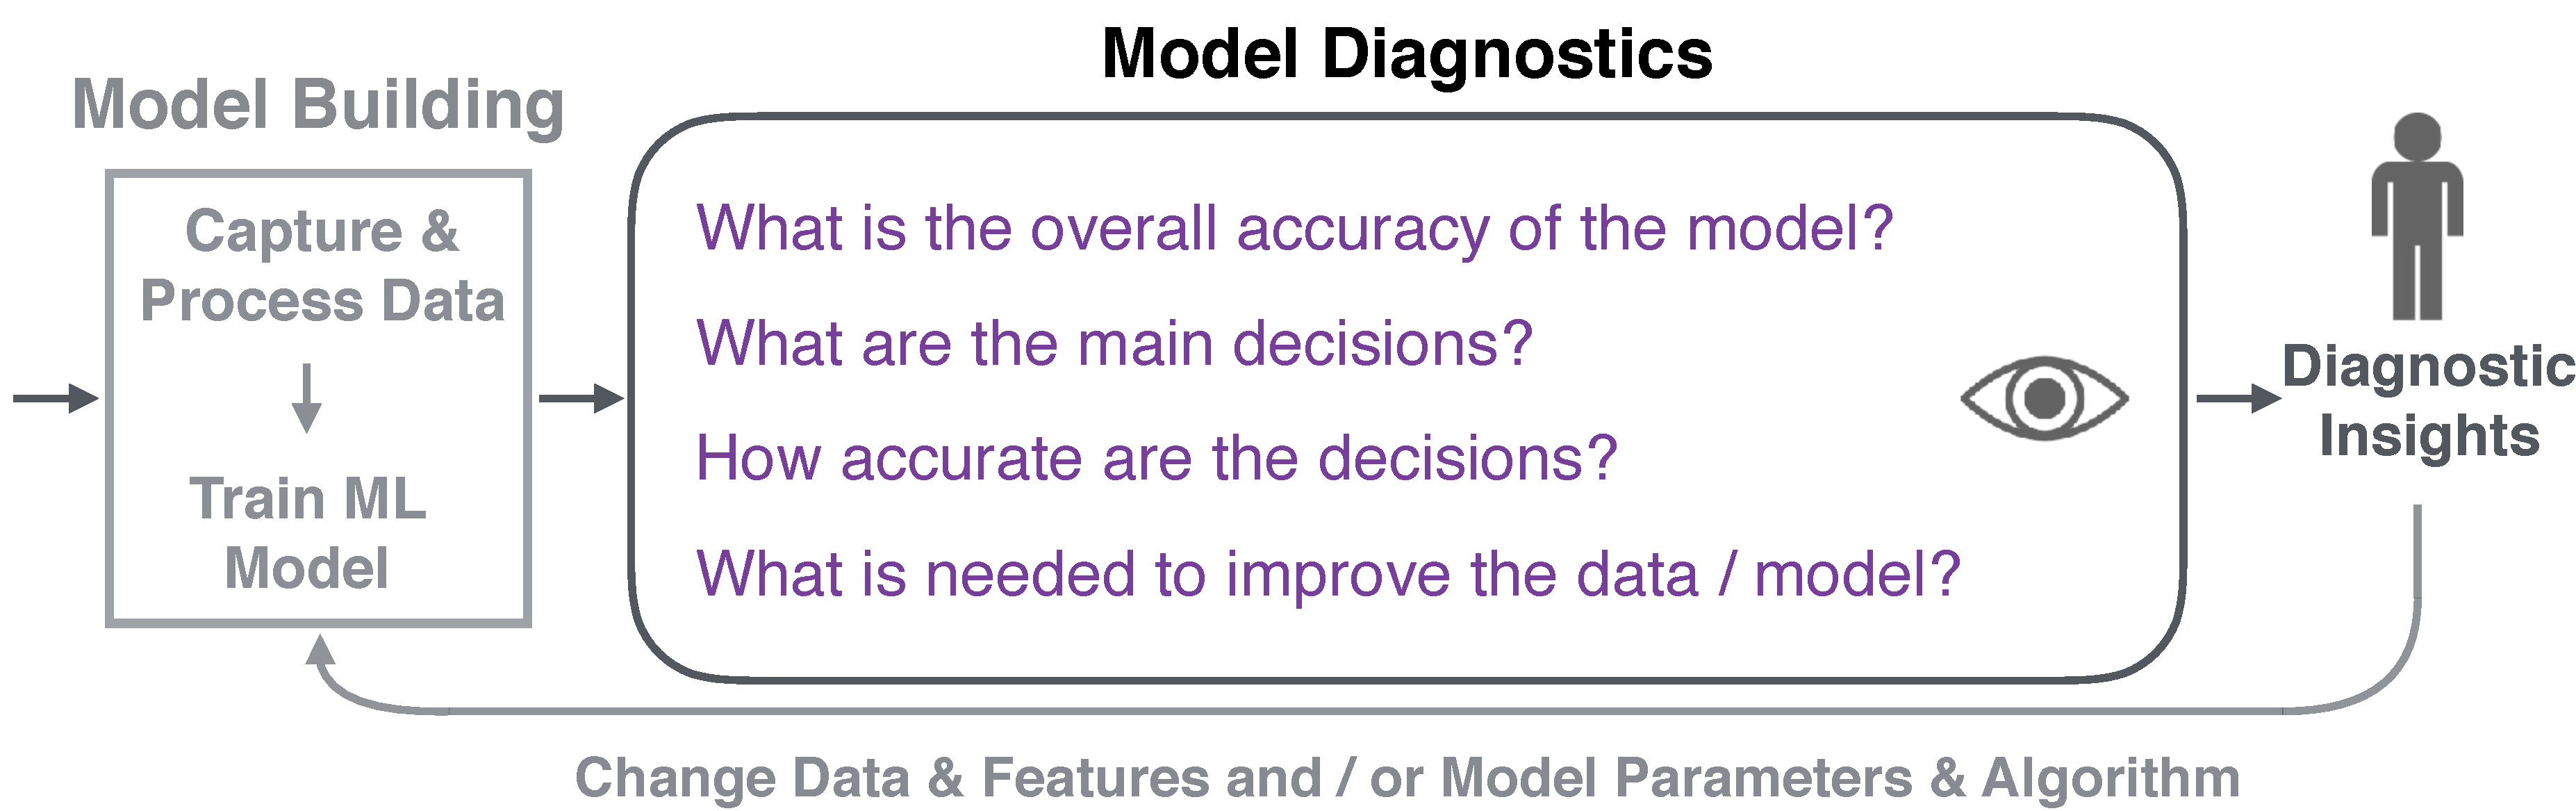
\includegraphics[width=\textwidth]{figs/workflow_large}
\caption[The model diagnostic workflow.]{
The proposed \textit{model diagnostic} workflow extends the conventional \textit{model building} workflow in machine learning for enabling domain experts to reason about the semantic validity of the decisions made by any model through multiple linked visualizations.
This ultimately helps to improve data acquisition and model generation processes belonging to the original workflow.
}
\label{figs:workflow_intro}
\end{figure}

% \section{Model Diagnostic Workflow}
In the third stage, we overcome this limitation by leveraging instance-level explanations. Instance-level explanations are defined as the smallest change, to an instance vector, necessary to change the predicted outcome label. Aggregating over those explanations and statistically analyzing the resulting instance subsets, proves as powerful novel approach for understanding the behavior of a model. Additionally, we propose a model diagnostic workflow (see \figref{figs:workflow_intro}) that helps identify flaws in the \emph{input data}, used to train and test the model.

We use this workflow to analyze a predictive modeling problem revolving patient admission to a hospital, of patients in the emergency department of said hospital. Accurately predicting whether a patient eventually gets admitted to the hospital helps reducing costs. The major limiting factor of this prediction task is the need for input features readily, and electronically, available at the earliest point possible. To this extend we initially used features of prescribed medications as this information is immediately available electronically. Our analysis showed that there are clear groups of patients where the predictive model is very helpful. However, there are some groups of patients where it is impossible for the predictive model to make accurate predictions given the provided information. One of those groups is patients receiving Diatrizoate Meglumine, a contrast medium for CAT or PET scans. This medication only indicates that a scan was performed, but does not carry information about the result of the scan. However, the result of the scan is the deciding factor whether a patient needs further care or can get sent home. Thus, with the given information it is impossible for the predictive model to make a decision that performs better than random guessing. Including more information in the form of additional features does indeed help with this problem but pushes the time when a decision can be made further back. One possible solution is to utilize the predictive model only for the confident groups of patients and wait for the doctors' decisions in other cases. This example illustrates that it is not only possible to \textbf{understand decision making} of a predictive model through the \textbf{model diagnostic workflow} based on \textbf{aggregated instance level explanations}, but also how it can be applied for \textbf{semantic validation} and \textbf{feature engineering} on the input data.

\begin{table}[t]
     \begin{tabular}{l|c|c|c} 
     \textbf{Approach} & \makebox[0pt][l]{\textbf{Instances}}\phantom{Aggregated} & \textbf{Aggregated} & \makebox[0pt][l]{\textbf{Global}}\phantom{Aggregated} \\ 
     \hline
     \hline
     \infuse & & & X \Tstrut\\
     \hline
     \prospector & X & & X \Tstrut\\
     \hline
     \textit{Model diagnostic workflow} & & X & \Tstrut\\
    \end{tabular}
    \centering
    \vspace*{-0.5em}
    \caption{Locality of decision analyses of the presented approaches. \textbf{Instances} refers to analyzing decisions for one instance at a time. \textbf{Aggregated} refers to analyzing decisions for groups of instances and \textbf{Global} refers to analyzing decisions globally without inspecting decisions for individual instances.}
    \vspace*{-0.75em}
    \label{tab:locality}
\end{table}

\todo{fill in latest work}
In addition to those promising results, there is still work to do.
It still needs to be shown that the proposed workflow of statistical analysis of instance-level explanations can be successfully applied to other data types than binary feature vectors, such as numerical features or highly redundant features such as found in images.
Early results in this direction indicate that it might be beneficial to abandon the focus on features to explain machine learning models, but rather focus on instances directly.
That is using instance-level explanations to obtain groups of \emph{instances} with similar behavior and then visualize those groups (\eg, using techniques proposed by \cite{seekaview}) in order to \emph{implicitly} explain them.
This provides more flexible explanations than those proposed earlier as their capability goes beyond ``Feature A and feature B positively impact the prediction for this group of instances" to also allow insights of the form ``The number of circles formed by black pixels contribute positively to the prediction" which would be very difficult to formulate by a machine but are easily formulated by humans using visualizations.
Furthermore, we are going to run a study on the implications on confidence in and trust of machine learning models when using different explanation approaches.
\todo{END?}

%%%
%  Furthermore, a formalization or taxonomy of common machine learning modeling \emph{errors} in both the modeling and feature engineering steps is needed to fully determine the limitations of the proposed black-box analysis methodologies. This can be achieved by taking a survey with both machine learning and domain experts to get an understanding and relevance of different kinds of those errors.
%%%

% Machine learning is a powerful tool that is used more and more in everyday life.
% By relating independent features and targets by detecting complex associations machine learning
% helps human decision making and, in some cases, even replaces it.
% Predictive modeling using classification techniques is a very common application of machine learning.
% In this work we will primarily focus on classification but the techniques discussed can, to some extent, be
% applied in other areas of machine learning as well.

% \begin{figure}
\centering
\vphantom{7cm}
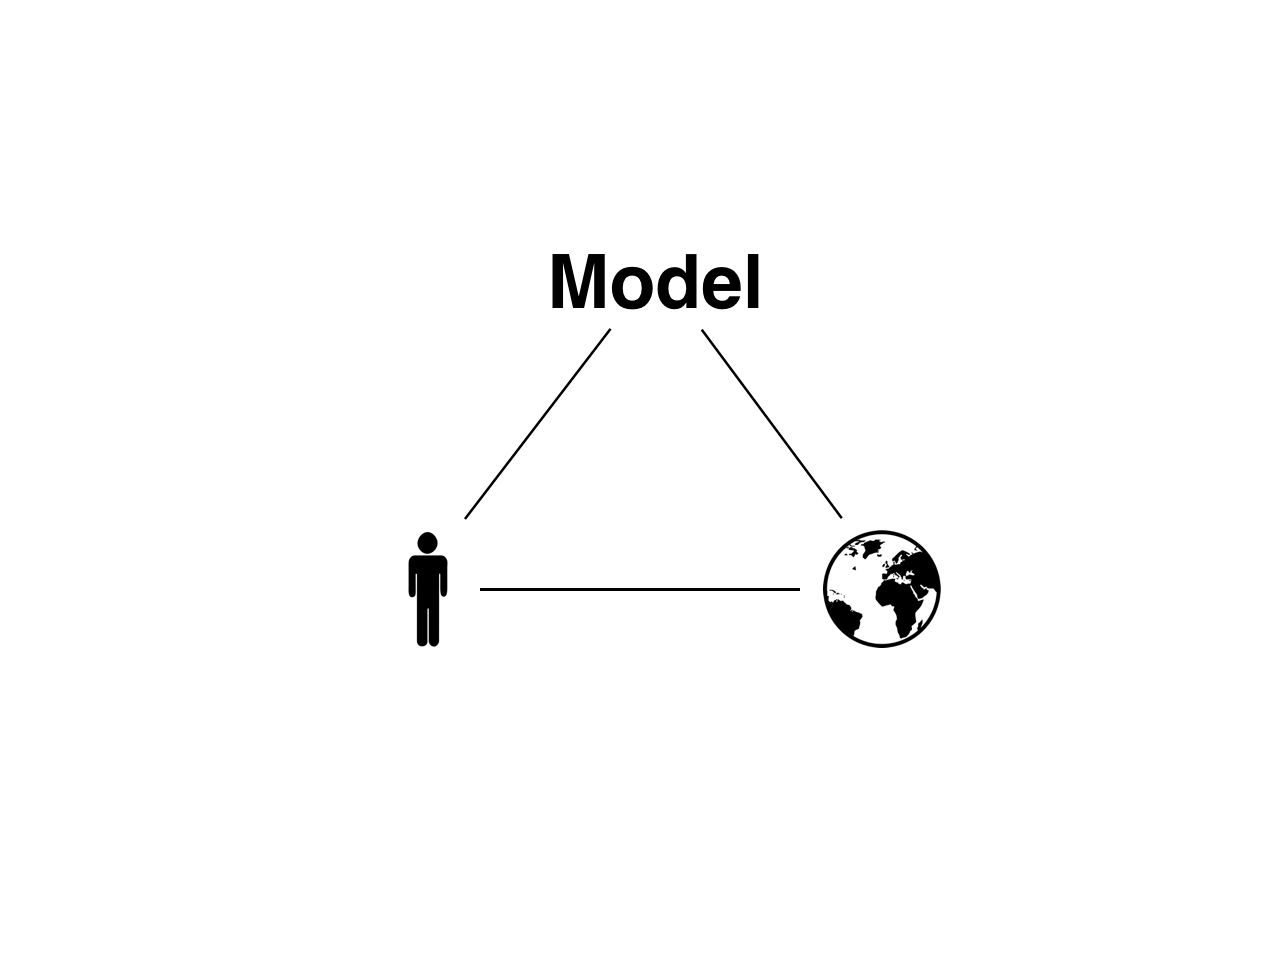
\includegraphics[trim={7cm 8cm 7cm 8cm},clip=true,width=0.275\linewidth]{figs/motivation/hmr}
~
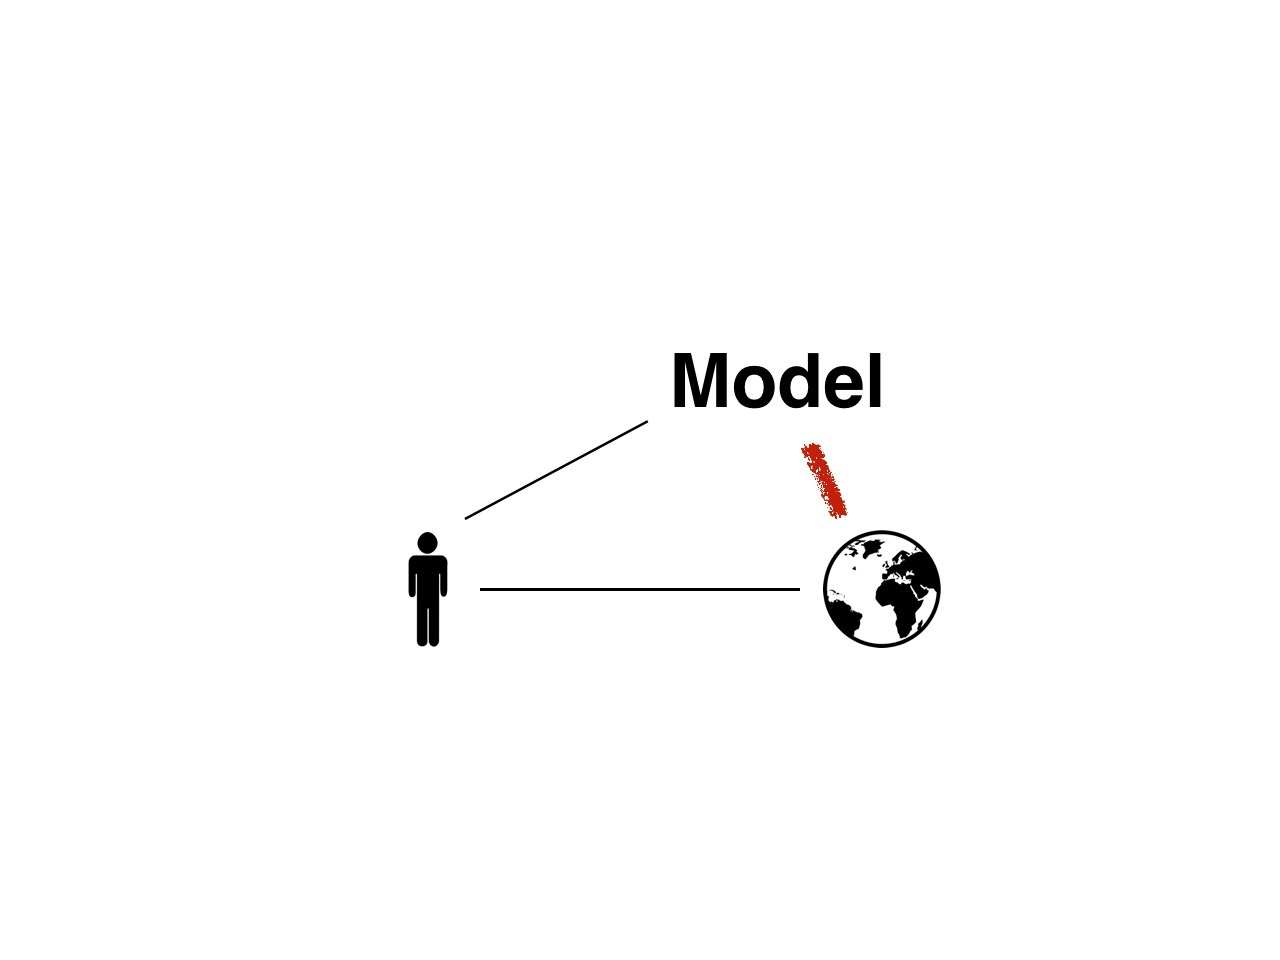
\includegraphics[trim={7cm 8cm 7cm 8cm},clip=true,width=0.275\linewidth]{figs/motivation/hmr_complex}
~
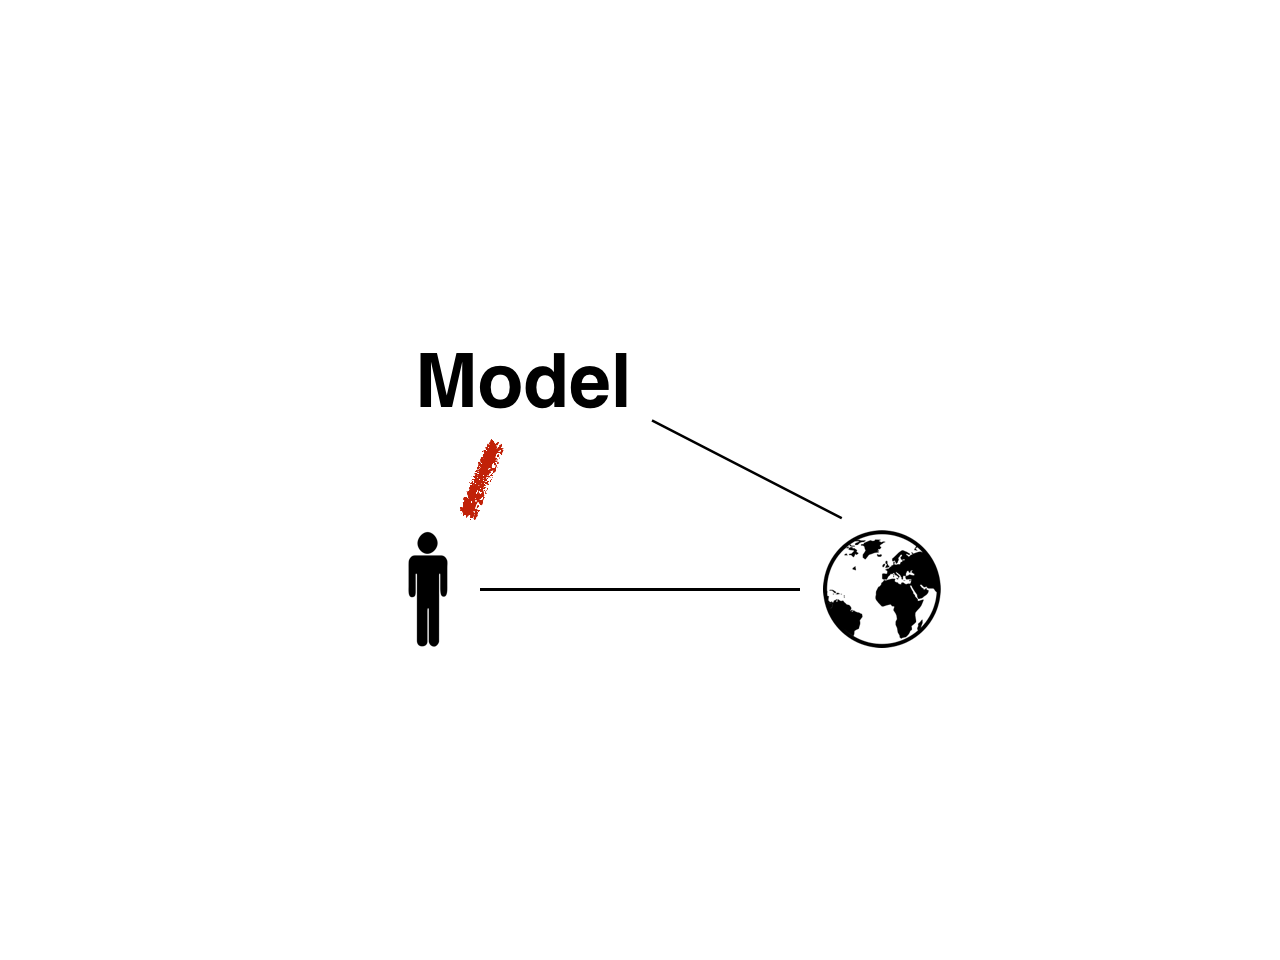
\includegraphics[trim={7cm 8cm 7cm 8cm},clip=true,width=0.275\linewidth]{figs/motivation/hmr_interpretable}
\caption{
Humans (lower left) build machine learning models (top) to understand and
predict reality (lower right). The second image illustrates how improving
machine learning models (ie., closing the gap between the model and reality)
makes it harder for humans to understand it. Likewise, simplifying the model
(ie., closing the gap between the model and the human) makes the model less
accurate (third image).
}
\label{figs:motivation_hmr}
\end{figure}

% As the scope and usage of machine predictions increases with bigger and more complex data
% the used algorithms need to also become more complex.
% However, as complexity increases it becomes harder for humans to follow the machine's decision making
% as illustrated in \figref{figs:motivation_hmr}.
% This problem of model transparency and interpretation is important and very well recognized in machine learning,
% as models with high predictive performance generally have low transparency and vice-versa~\cite{breiman2001}.

% \begin{figure}
\centering
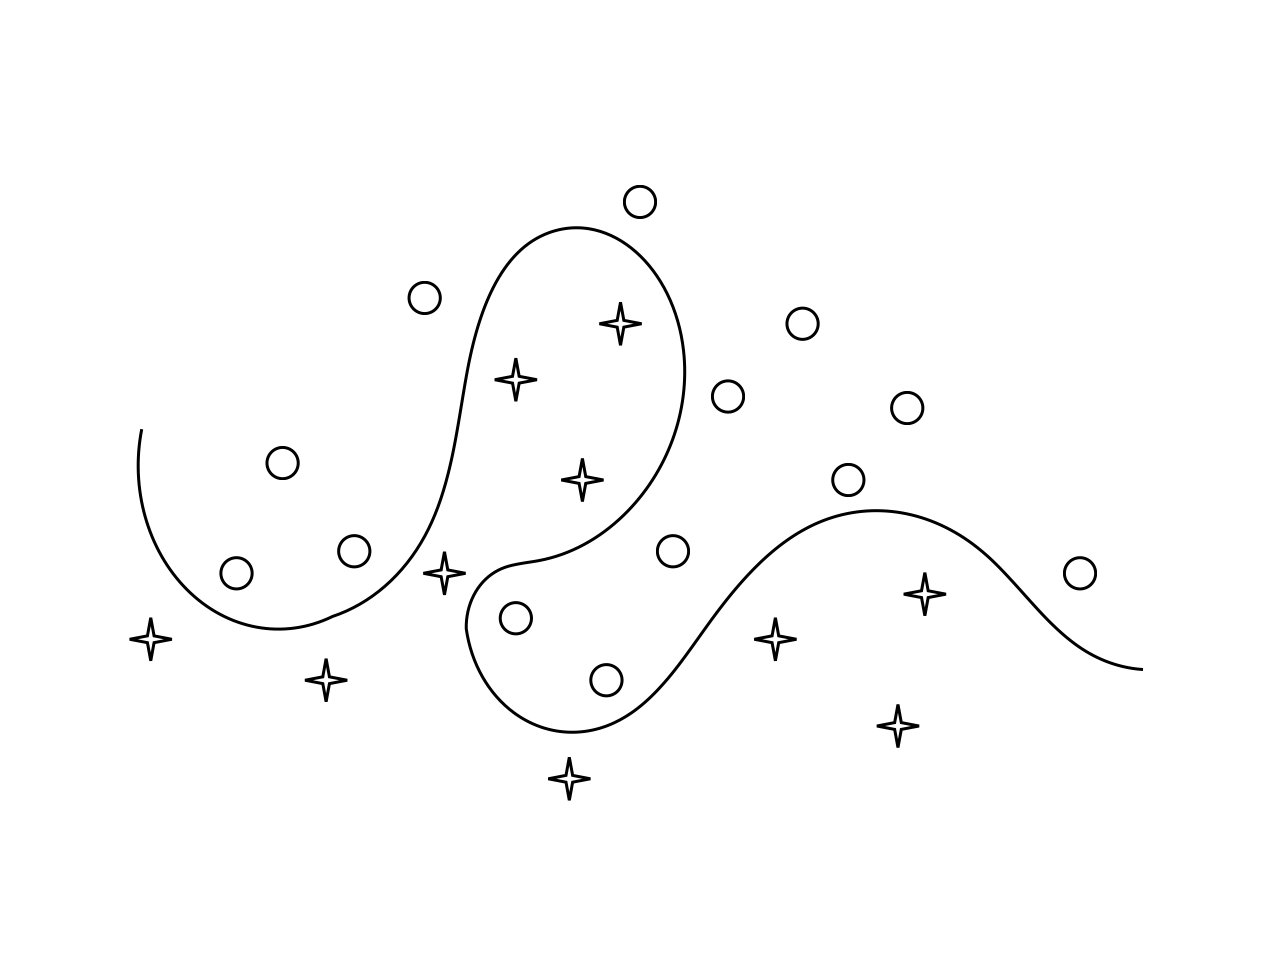
\includegraphics[height=10.5em]{figs/motivation/ml_orig}
\raisebox{4.75em}{$\Rightarrow$}
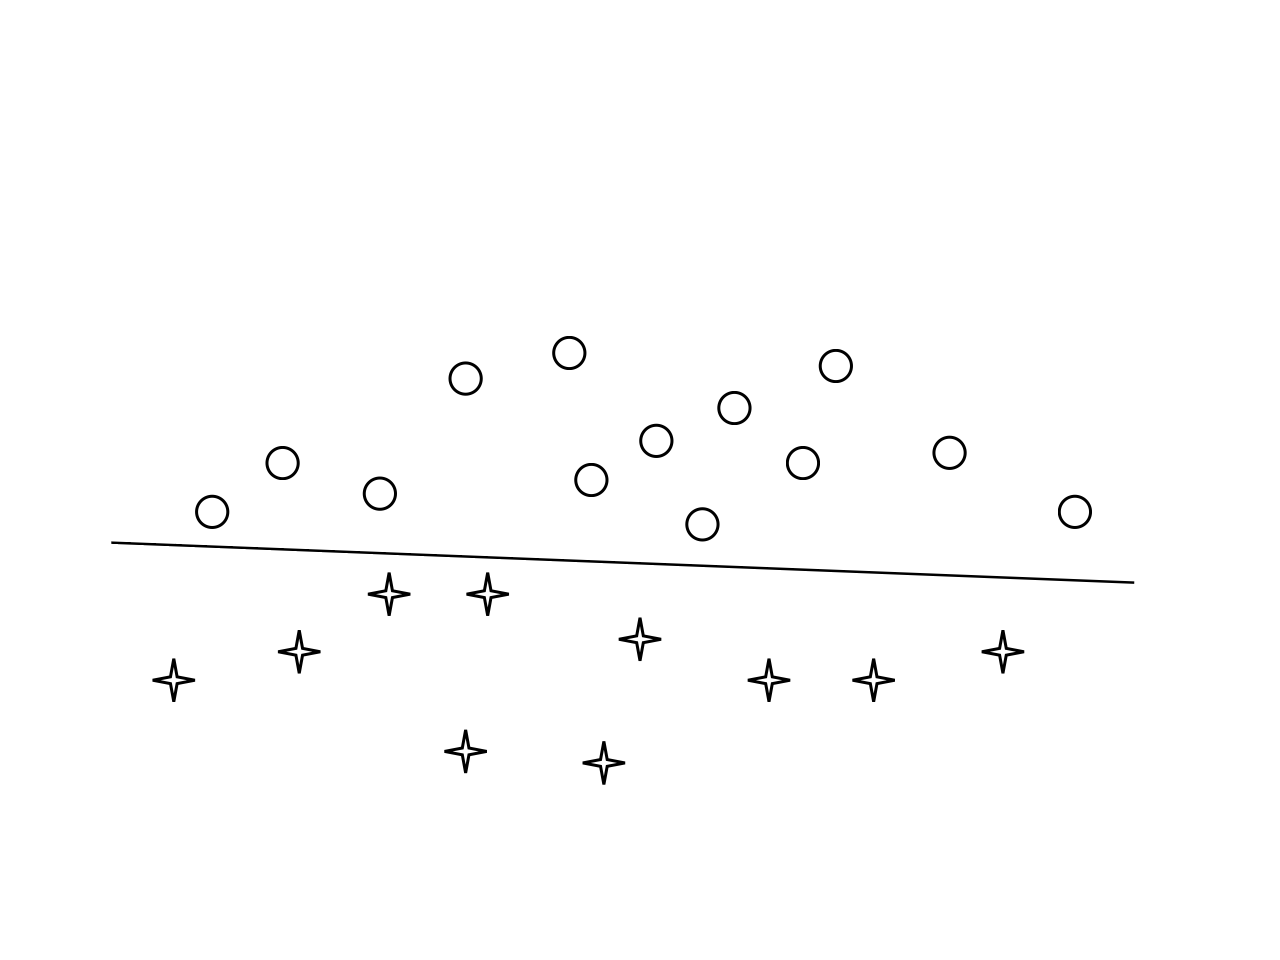
\includegraphics[height=10.5em]{figs/motivation/ml_proj}
\caption{
Machine learning algorithms transform the complex raw input space (left)
into a cleaner transformed space (right) that can be easily separated.
Transformations are often strongly non-linear, non-affine, and/or non-continuous
and thus not easy to follow or understand.
}
\label{figs:motivation_ml}
\end{figure}

% Many applications of machine learning need to be interpretable to humans even though
% sacrificing prediction performance is not desirable.
% For example, in the health care domain disease prediction using patient histories needs to be fully
% transparent and comprehensible to practitioners as lives are at stake when applying models in the real world.
% Even if a model performs well on the test data it could draw its conclusions from hidden signals or biases
% in the training data. We found many of such examples in the work presented here.

% One way of overcoming the problem of interpretability vs. performance in machine learning is to
% break down the complex models into smaller parts that are easier to understand (see \figref{figs:motivation_ml}).
% While this reduces the complexity it also reduces the generalizability of the explanations created this way.
% In the following we will explore when explanations are useful and how they can be used.

% \section{Explanations}
% Explanations for machine learning can be desirable for multiple reasons:

% \begin{description}
%     \item[Liability]
%         Decisions made by the machine have real world consequences with attached liabilities.
%         Explanations are needed to create confidence that the model avoids costly misjudgements of critical inputs.
%     \item[Trust]
%         Stakeholders need to be able to trust decisions from the model.
%     \item[Debugging]
%         Help understanding why a model behaves different than expected.
%     \item[Comparison]
%         Provide a model agnostic way of comparing different models.
%     \item[Hidden Associations]
%         Find hidden associations in the original data.
%     \item[Ambiguity Reduction]
%         By creating generalizing models and explaining their behavior a noise-free view of the data can be created.
% \end{description}

% Those explanation tasks can be performed at different steps in the machine learning process.
% In this context predictive modeling typically consists of three steps (see \figref{figs:motivation_flow}).
% First, the input data has to be prepared.
% This entails choosing which data points are eligible for modeling to ensure that no inherent biases influence
% the validity of the created model.
% Furthermore, data usually needs to be converted into features that can be used by machine learning models.
% Second, the model has to be trained on the transformed data.
% Depending on the type of the model or strategy this step includes splitting the data into cross-validation sets,
% algorithmic feature selection, and actually training the model.
% Third, the actual prediction can be performed which often entails converting class probabilities into
% concrete labels upon which decisions can be performed.

% Explanations can be separated into different categories that utilize and describe
% different stages of the predictive modeling pipeline.
% Thus, explanations can be divided into input-, output-, interaction-,
% and structure-explanations.
% Input explanations mostly work with the raw input data and can help the pre-processing.
% Output explanations analyze outputs from the machine learning model such as feature ranks
% or prediction scores.
% Interaction explanations change model inputs to observe how the corresponding model output
% changes.
% Structure explanations describe the inner values and weights of a model so decisions
% can be followed manually.

% \begin{figure}[b!]
\centering
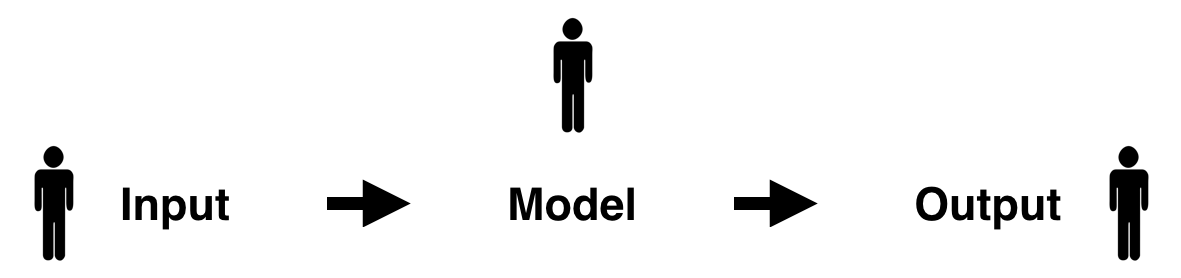
\includegraphics[width=0.7\linewidth]{figs/motivation/flow}
\caption{
The predictive modeling pipeline.
Humans symbolize where explanations are helpful.
Explanations of the model can either focus on input-output interactions
or the structure of the model.
}
\label{figs:motivation_flow}
\end{figure}

% Output and interaction explanations can also utilize model induction, which is building
% a less complex model on top of the original model's output or on a strategically chosen
% subset of data points.
% This less complex model can then be structurally described which is beneficial when
% dealing with very complex models whose structural explanations are too difficult to
% understand.

% \begin{figure}
\centering
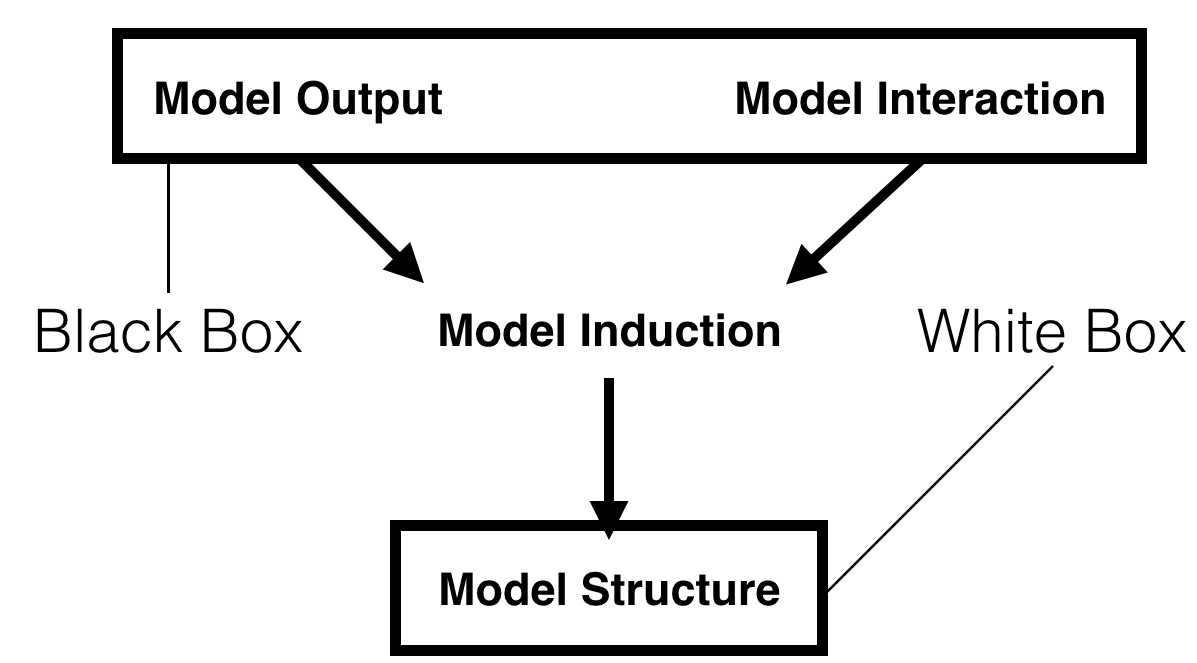
\includegraphics[height=11em]{figs/motivation/expl_classes}
\caption{
The relation of output-, interaction-, and structure-explanations.
With the help of model induction over a reduced or carefully selected
input, output- and interaction-explanations can utilize structure explanations
of simple machine learning models.
Output- and interaction-explanations can be created while treating the model
as black-box. This is not possible for structure explanations.
}
\label{figs:motivation_expl_classes}
\end{figure}

% The types of explanations can be broadly categorized into black box (output and interaction)
% and white box (structure) explanations as shown in \figref{figs:motivation_expl_classes}.
% Note that input explanations do not fall into either of those categories as they
% do not rely on any \emph{concrete} machine learning model due to focusing on data
% preparation and pre-processing.

% In this work we discuss exclusively input and black box explanations.
% Black box-, as opposed to white box-, explanations have the advantage that they can
% deal with any complexity of the underlying model.
% Developed techniques also do not need to be adapted to new algorithms emerging from
% machine learning research as long as the core interface (input produces prediction scores)
% remains the same.
% Furthermore, black box explanations also allow to compare the behavior of different
% algorithms which is otherwise not possible.
% Lastly, with good performing machine learning models being highly valued in certain
% domains stakeholders do not need to fully reveal their assets to analysts using
% black box explanations.

% \section{Overview}
% In the following we show how the previously mentioned different kinds of explanations
% can be utilized using tools we developed.

% At first we focus on tools that help with the data preparation step.
% SeekAView (see \chapref{sec:SeekAView}) helps detect unusual patterns in the data and
% provides a way to find associations between features using guided subspace analysis.
% With Patient-viz (see \chapref{sec:Patient-viz}) we show a tool to verify the integrity
% of patient records that are used to construct features for diagnosis prediction.
% The tool helped a group of machine learning modelers and practitioners refine their definitions for disease labels.
% COQUITO (see \chapref{sec:COQUITO}) is designed to ease cohort definition and construction in the medical context.

% \begin{figure}[b!]
\centering
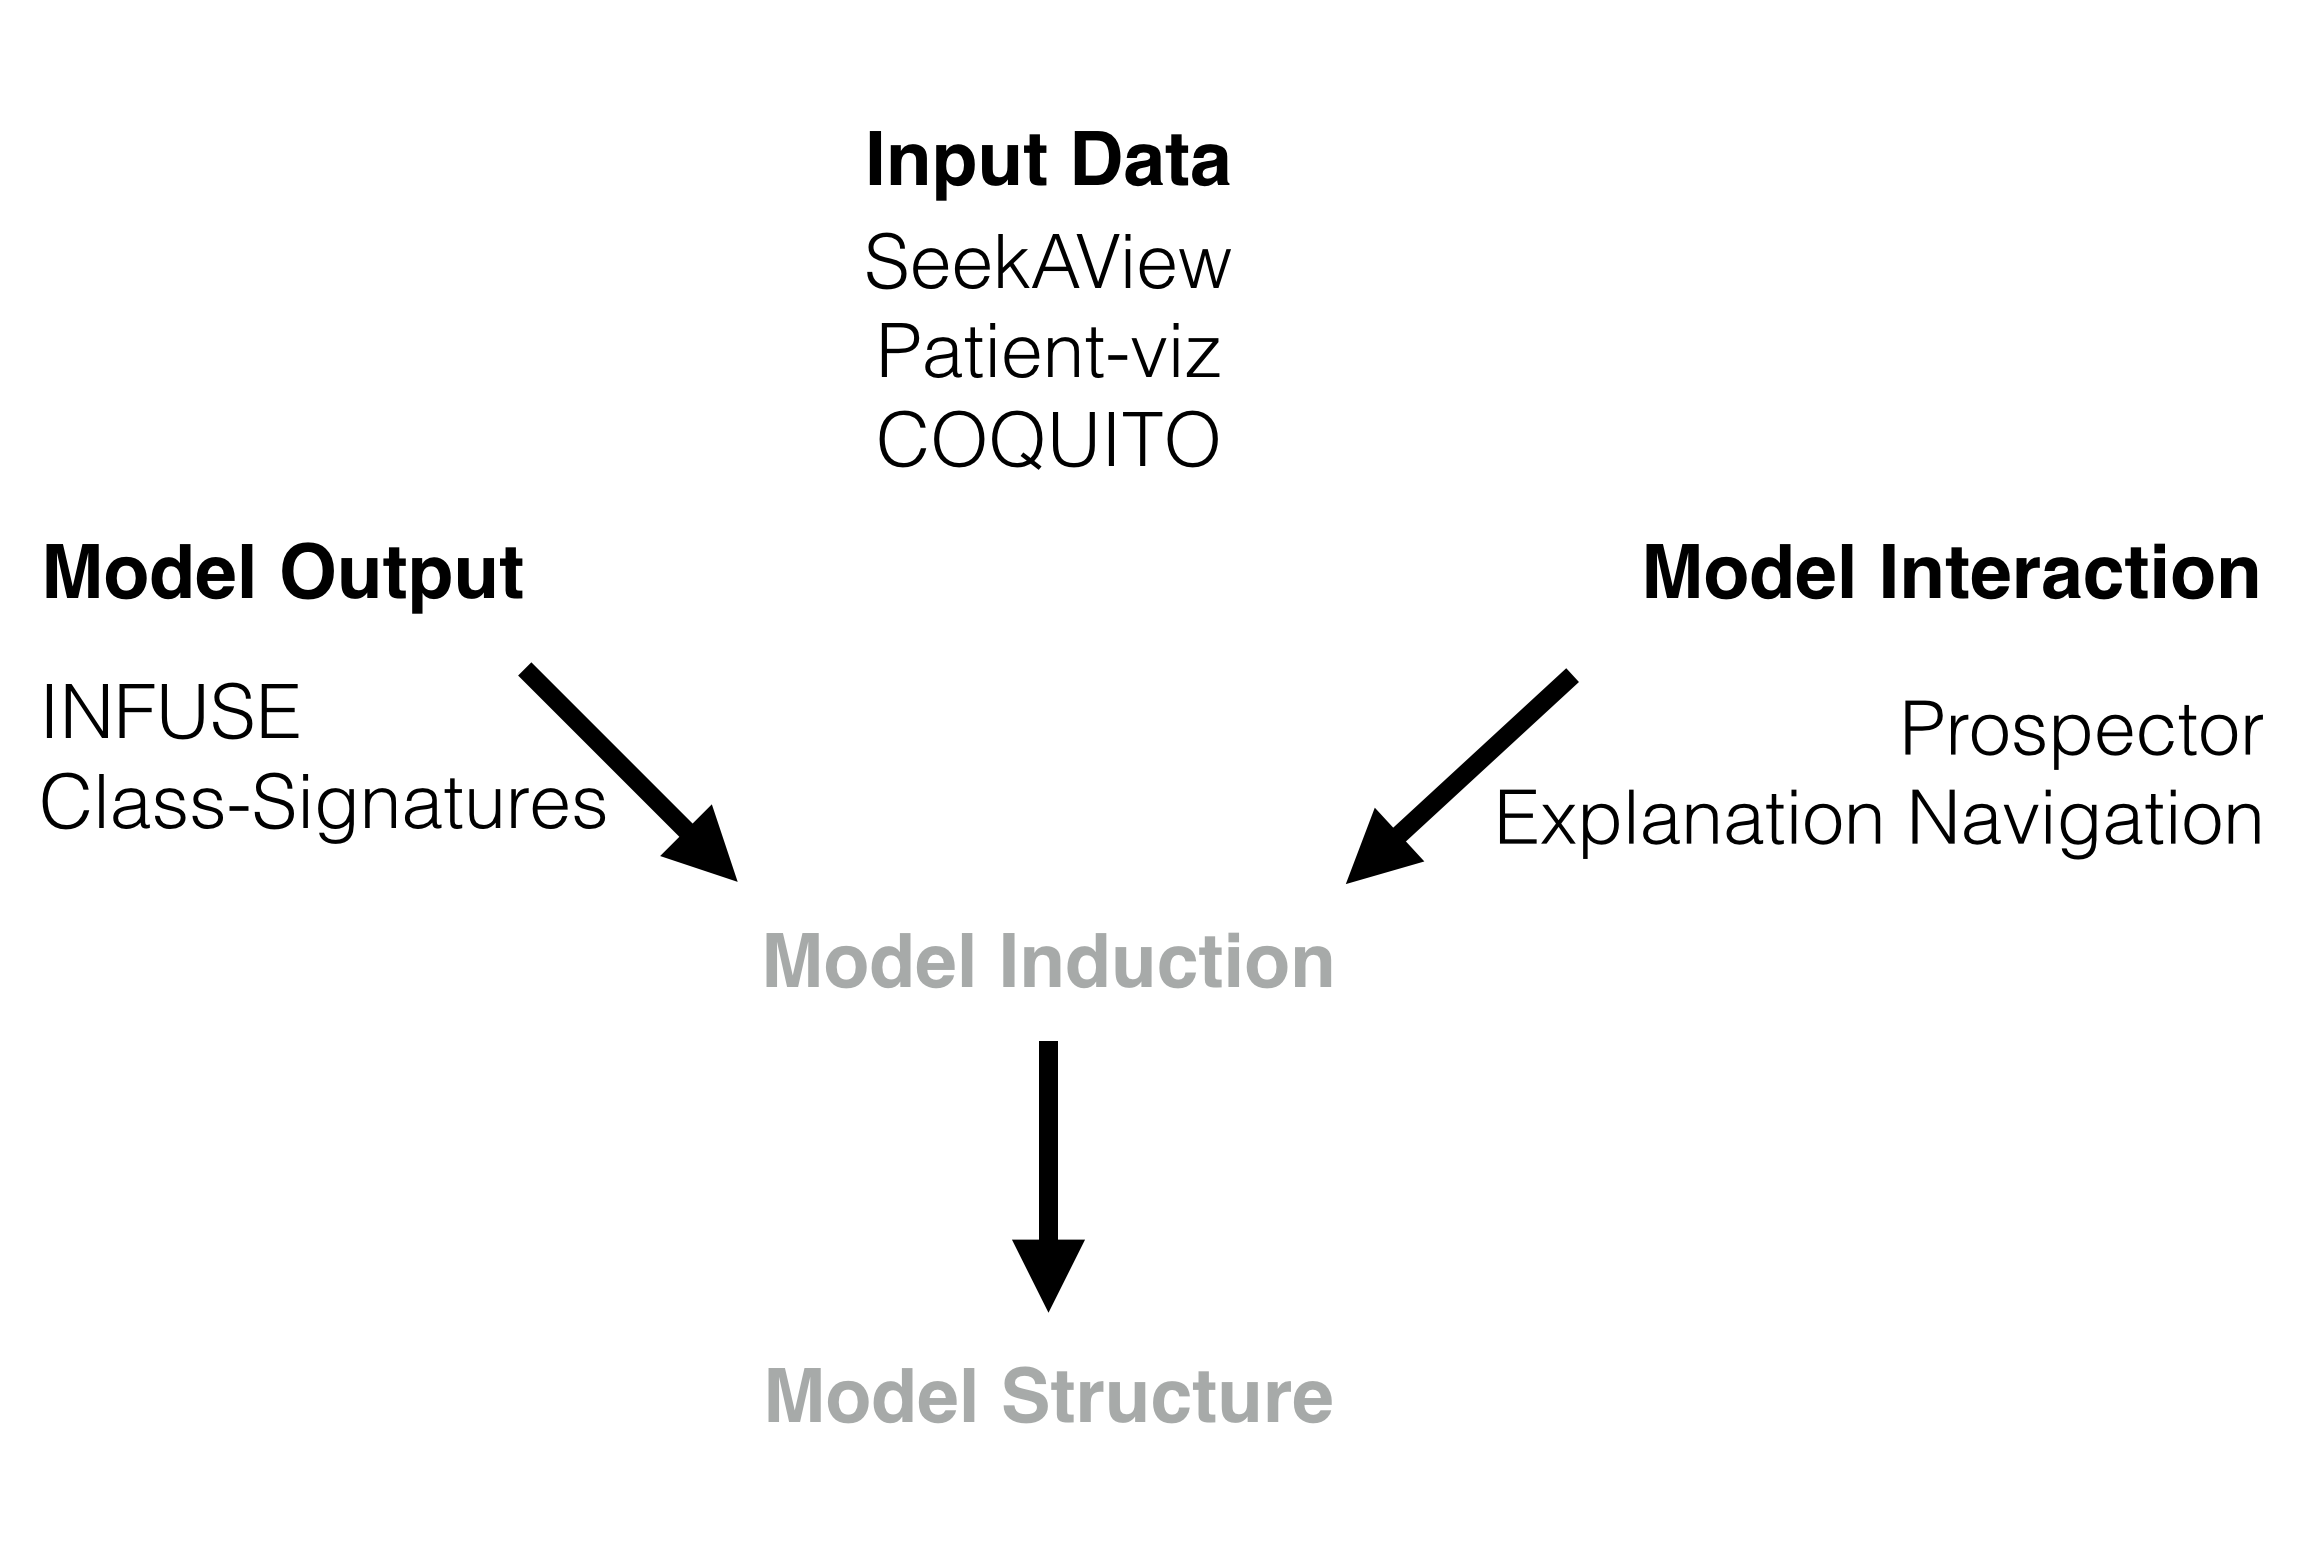
\includegraphics[height=14em]{figs/motivation/content}
\caption{
How the projects of my dissertation fit into the categorization of explanations
as shown in \figref{figs:motivation_expl_classes}.
As input data is focused on data pre-processing it doesn't appear in the
original figure. Furthermore, no works focusing on structure explanations are
presented as they require knowledge about the internal state of the model.
However, with \textbf{Class Signatures} model induction based on the original
model's outputs and subsequent structure explanations of the induced model are
part of the work-flow.
}
\label{figs:motivation_content}
\end{figure}

% Secondly, we focus on tools that use model interaction to explain model behavior.
% Those techniques search the output space of a model by manipulating the input space and differ mostly
% by their mechanism of probing the machine learning model.
% Prospector (see \chapref{sec:Prospector}) uses partial dependence to calculate the local
% influence of features.
% We are currently working on a tool that uses a different probing mechanism aimed at
% textual data which is described in \chapref{sec:Outlook}.

% Thirdly, we focus on tools using only the output of machine learning models to
% provide explanations.
% This category is especially useful if the model that produced the output cannot
% be shared or is otherwise not be available.
% The scope of model outputs can reach from feature rankings as shown with INFUSE (see \chapref{sec:INFUSE})
% to analyzing predictions scores (see \chapref{sec:Class-Signatures}).
% The latter is partially published ongoing work which we will revisit in \chapref{sec:Outlook}.

% In \chapref{sec:Outlook} we will describe current projects that fit in the categories described above.
% We further explore in which directions those projects develop and provide a time-line of their completion
% alongside a draft of final thesis' structure in \chapref{chap:outline}.

\section{Machine Learning and Predictive Modeling}
Machine learning enables computers to perform tasks without manually codifying all instructions.
This automated programming makes machine learning a popular and widely used approach for many applications as it provides a time- and cost-effective alternative to manually created software solutions.
Machine learning relies on algorithms that learn and generalize from examples in order to perform accurately on new or unseen data.

Predictive modeling is a subcategory of machine learning that aims to predict certain properties from given input data.
The input data typically consists of \emph{instances} with a given set of \emph{features}.
The values of those features can be binary, categorical, or numerical.
We can think of the data as a table where features are columns and rows are instances.
Thus, this kind of data is typically referred to as \emph{tabular} or \emph{structured} data.
In the case of \emph{unstructured} data, such as plain text, the data needs to be converted into structured data first, before it can be used as input of predictive models\footnote{In this case, the model input corresponds to a fixed-length transformed representation of the original input data. These transformations can be either learned (\ie, via deep learning or similar methods) or are manually specified.}.
The predicted property, \emph{outcome} or \emph{label}, can be numerical, in which case the task is called \emph{regression}, or categorical, in which case the task is called \emph{classification}\footnote{A combination of multiple properties are also possible to predict, in which case the task is called multitask learning, structured learning, \etc. Currently, the most common form of predictive modeling involves either a single classification or single regression task.}.
The different values the label can assume are called \emph{classes}.
The task is call \emph{binary classification} if the categorical label has exactly two classes.

The predictive model learns by \emph{training} with a set of example instances (\emph{training set}) and their associated labels.
In order to verify that the model did indeed correctly learn from the given examples, a second, previously unseen, set of example instances (testing or \emph{validation set}) with known labels is typically used.
The model is used to predict the labels of this set which are then compared to the actual labels of those instances.
Various statistical measures can be computed on this relationship between the predicted and actual labels \cite{mlbook}.

For binary classification tasks (for simplicity \emph{positive} and \emph{negative} are used below to describe the outcomes) those statistical measures include:

\begin{description}[noitemsep]
    \item[True Positive / Negative]
    The number of correctly predicted positive ($TP$) or negative instances ($TN$).
    \item[False Positive / Negative]
    The number of incorrectly predicted positive ($FP$) or negative instances ($FN$).
    \item[Accuracy]
    $(TP + TN) / (TP + TN + FP + FN)$ The proportion of correctly predicted instances.
    \item[Precision]
    $TP / (TP + FP)$ The ratio of correctly predicted positive instances to instances which were predicted to be positive.
    \item[True Positive Rate / Recall]
    $TP / (TP + FN)$ The proportion of correctly predicted positive instances.
    \item[False Positive Rate]
    $FP / (FP + TN)$ The proportion of incorrectly predicted positive instances.
\end{description}

Additionally, a further model quality measurement can be derived from the confidence of a model in its prediction.
Typically, classification models allow to output probabilities for each class instead of the predicted class directly.
This allows for inspecting the \emph{confidence} of the model.
In the case of binary classifiers a \emph{threshold} can be used to adjust predictions to favor confidence in a certain class higher than the other.
This is achieved by outputting the positive class as prediction if its probability is higher than the threshold and the negative class otherwise.

\begin{figure}
\centering
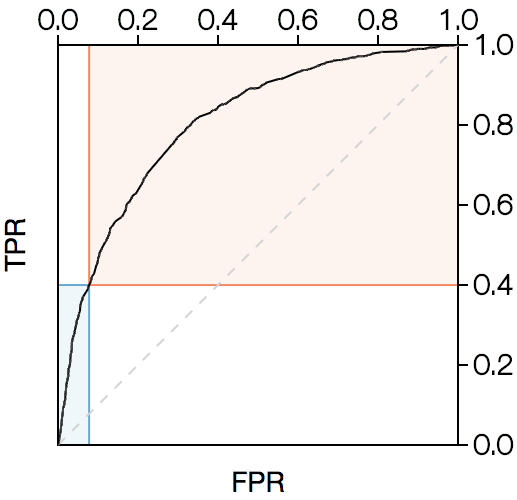
\includegraphics[height=10em]{figs/roc}
\caption[Example of a ROC curve.]{
Example of a ROC curve. The threshold minimizing incorrect predictions is highlighted by the colored axes.
}
\label{figs:roc_intro}
\end{figure}

The \emph{receiver operating characteristic} (ROC) curve for binary classifiers plots the true positive rate against the false positive rate for all thresholds between $0$ and $1$.
The plot indicates the correctness of the model \wrt its confidence.
The ROC curve for a perfect model ($100\%$ accuracy) would follow the left vertical axis and the top horizontal axis.
The area under the ROC curve (\emph{AUC}) is a commonly used measure for model quality \cite{bradley19971145}.

\subsection{Popular Algorithms}
There are too many algorithms for predictive models to list all of them here.
However, following we will discuss the most commonly used algorithms.

\subsubsection{Logistic Regression}
Logistic Regression \cite{mlbook} is one of the most popular algorithms in machine learning.
This is due to its simplicity and its interpretability of the results.
Suppose $x_i$ is the value of the feature $i$ of our data, a binary classification using Logistic Regression is equivalent to:
\[
l(x) = b + \sum_{i \in \mathcal{C}} w_i x_i
\]
where $\mathcal{C}$ is the set of features, $b$ and $w_i$ are the learned weights of the model, and the outcome is determined by whether the weighted sum $l(x)$ is larger or smaller than zero.
In order to work with probabilities, have greater precision around the boundary, and to penalize points close to the boundary, a logistic function is used:
\[
P(Y=1 | x) = L(x) = \frac{1}{1 + e^{-l(x)}}
\]
which gives the likelihood of one of the classes.
In order to train the model, \ie, finding the best values of $b$ and $w_f$, the expression $P(Y=y | x)$, where $y$ represents the ground truth 0 or 1 of the training instances, needs to be maximized.
In practice, instead of maximizing $P(Y=y|x)$, the negative logarithm of this expression is minimized.
When optimized over the entire training data, this expression is called \emph{negative log likelihood} and it can be optimized via techniques such as gradient descent, to find optimal values of $b$ and $w_f$.

One of the main advantages of logistic regression is its interpretability.
The weights $w_i$ can be directly interpreted as how influential a particular feature is.
That is, if the magnitude of a weight is large, a small change in the value $x_i$ of the feature has a big impact on the overall sum.
Additionally, the sign of a weight indicates whether a particular feature is positively or negatively correlated with the outcome.
For example, a simple (not necessarily correct) predictor for Type 2 Diabetes\footnote{A disease, affecting the body's ability to regulate blood sugar, which is mostly driven by lifestyle choices and associated with obesity and hypertension. The most common age of onset is between ${\sim}45$ and ${\sim}65$.} could look like:
\[
l_\text{diabetes}(x) = -1.9 + 0.01 x_\text{age} + 0.02 x_\text{mass} + (-0.3) x_\text{height}
\]
with $x_\text{age}$ in years, $x_\text{mass}$ in \si{kg}, and $x_\text{height}$ in \si{m}.
From here, we can see that the model assumes that a high mass leads to higher Diabetes risk, old age also leads to a higher risk but less so than high mass, and large body height leads to a smaller risk.
This gives a very intuitive understanding of how the model is reaching its conclusion.

However, this example also illustrates some limitations of logistic regression models.
BMI (Body Mass Index; $x_\text{mass} / x_\text{height}^2$) is a better indicator than mass or height alone, but cannot be expressed or learned by a logistic regression model\footnote{Note, that we could provide BMI directly but only because domain experts had inferred the importance of this relationship in the past. Alternatively, we could also provide features in logarithmic space enabling logistic regression models to learn this relationship, since logarithmic BMI is $\log{(x_\text{mass})} - 2.0 \log{(x_\text{height})}$.}.
Additionally, since the influence of the features is always the same, one feature can force a prediction if its values are large enough.
For example, the model will predict a high Diabetes risk with high age independent of the mass or height.

\subsubsection{Generalized Additive Models}
A Generalized Additive Model (GAM \cite{gam}) extends the idea of logistic regression to functions instead of weights:
\[
g(x) = b + \sum_{i \in \mathcal{C}} f_i(x_i)
\]
where $\mathcal{C}$ is the set of features, $b$ is the learned bias of the model, $f_i$ are learned influence functions, and the outcome is determined by whether the sum $g(x)$ is larger or smaller than zero.
Having influence functions overcomes the restricted expressiveness of logistic regression models while maintaining its interpretability.
The impact of individual features can be seen in the plots of the influence functions.

\begin{figure}
\centering
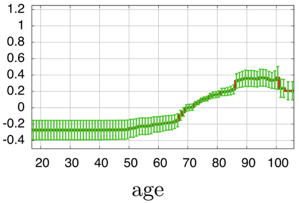
\includegraphics[height=8em,valign=t]{tex/introduction/age.png}
\caption[Influence function for ``age" from a Generalized Additive Model.]{
An influence function for ``age" from a Generalized Additive Model \cite{Caruana:2015:IMH:2783258.2788613}.
}
\label{figs:age}
\end{figure}

In the Diabetes example from above, a GAM could solve the issue of always connecting high age to high Diabetes risk by decreasing the influence of the feature age for higher values than ${\sim}65$.
However, since GAMs only consider one feature at a time, the BMI ($x_\text{mass} / x_\text{height}^2$) can still not be expressed or learned by the model.

\subsubsection{Decision Trees}
Instead of computing predictions with a mathematical formula, Decision Trees \cite{mlbook} determine predictions by following a sequence of tests on the data.
Decision Trees are trees where each node represents a test $x_i > t_i$, with $x_i$ as the value of the feature $i$ and $t_i$ as learned threshold.
The prediction algorithm starts at the root of the tree.
Depending on the outcome of the test in the root node the algorithm continues with the corresponding sub-tree recursively, until a leaf node is reached.
The leaf nodes contain the probabilities for the outcomes of the prediction task and are returned as result by the algorithm.

\begin{figure}
    \centering
    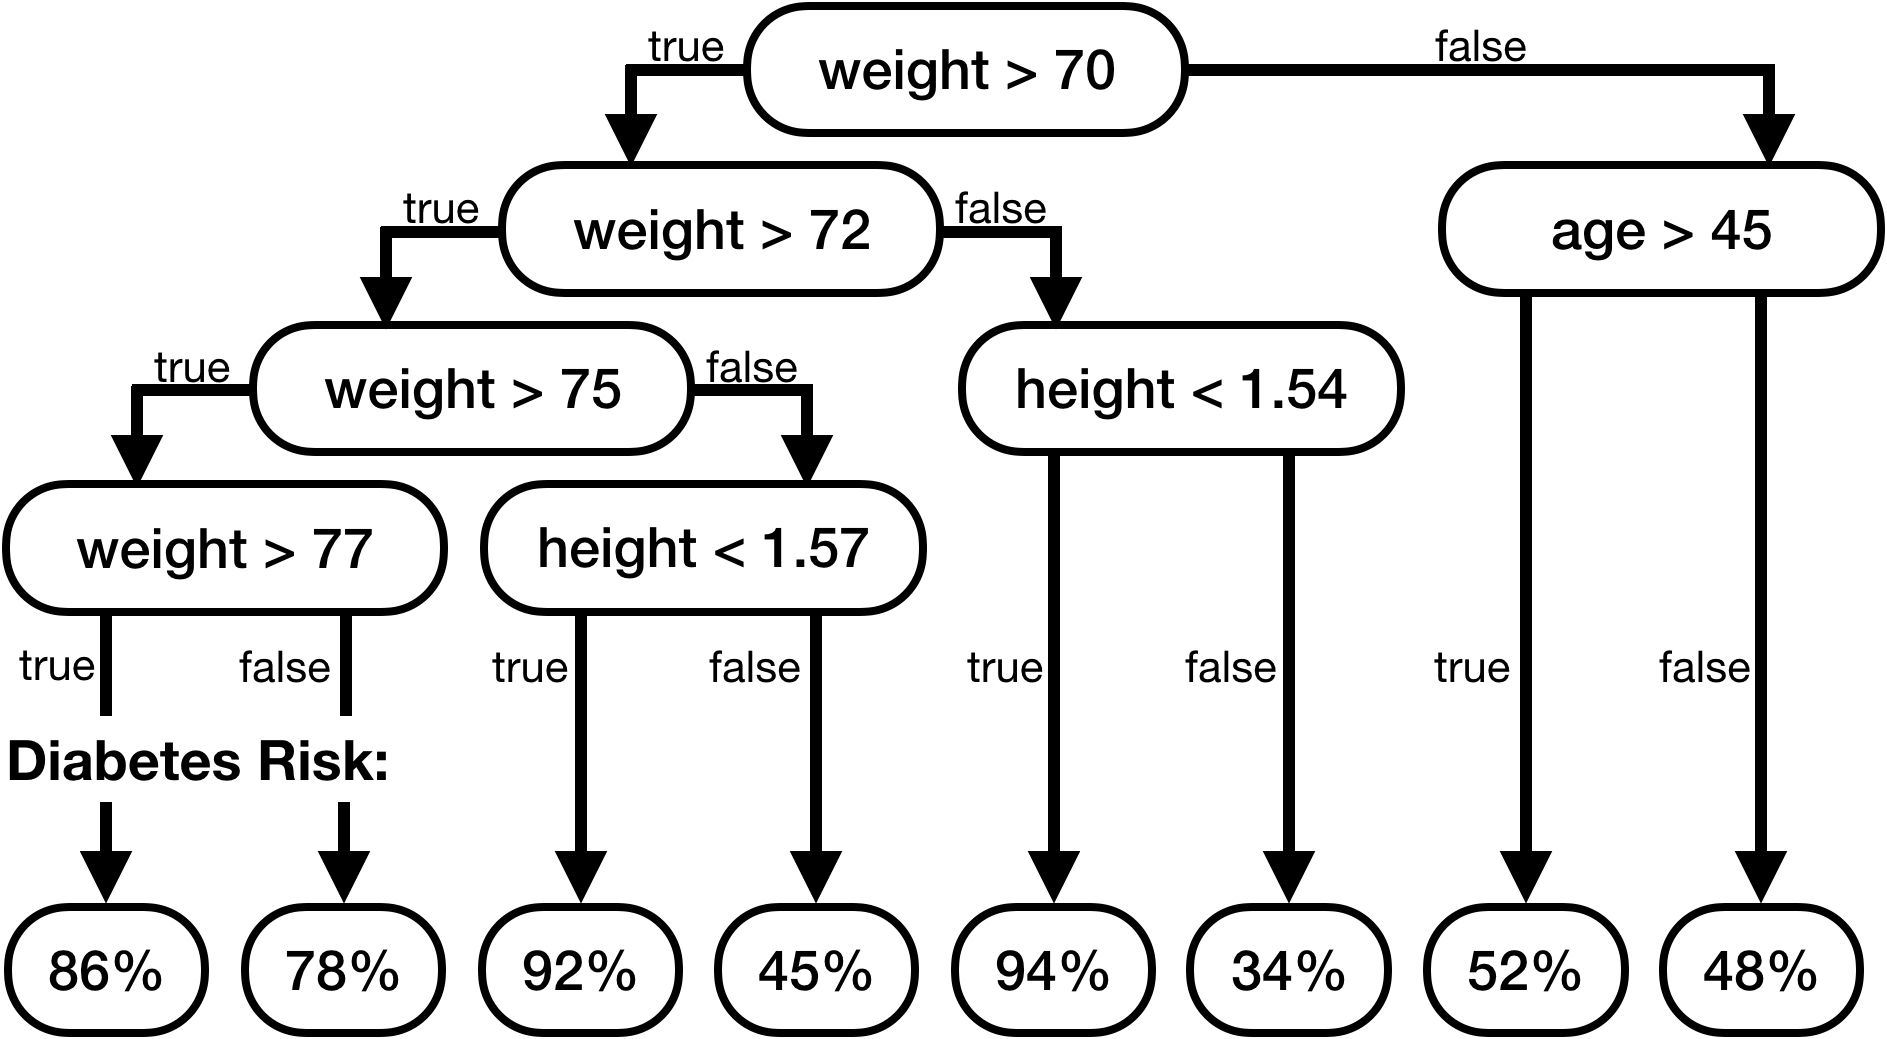
\includegraphics[width=0.9\linewidth]{tex/decisiontree}
    \caption[Example Decision Tree]{A possible decision tree for the Diabetes prediction example\footnotemark. Note, that the tree has interval checks to model the relationship between ``weight'' in \si{kg} and ``height'' in \si{m}.}
    \label{figs:dctree}
\end{figure}
\footnotetext{The decision tree or its parameters are \emph{not} based on data and serve only illustratory purposes.}

Decision Trees are usually considered very interpretable, as their behaviour is intuitively understandable.
However, this only holds true for trees with a relatively low number of nodes.
Trees with hundreds or thousands of nodes are hard to interpret as their complexity makes it hard to gain a mental model.

Decision Trees excel in cases where certain ranges of features have a clear impact on the outcome.
For example, in our running Diabetes use case, the risk of becoming diabetic is significantly higher for ages between ${\sim}45$ and ${\sim}65$.
A Decision Tree can then differentiate by age and infer the prediction differently for values inside or outside of that range.

However, Decision Trees cannot model relationships between features very well and have to approximate them.
For example, increasing the height of a person also increases that person's weight.
This means that whether a person is overweight, not only depends on the weight of the person, but also how tall that person is.
A person weighing $80\si{kg}$ can be considered overweight with a height of $1.7\si{m}$ but would not be with a height of $1.8\si{m}$.
Since a Decision Tree cannot model this relationship ($x_\text{mass} / x_\text{height}^2 \geq 25$) directly it has to approximate it by breaking the values of $x_\text{mass}$ and $x_\text{height}$ into intervals and checking them separately (see Figure~\ref{figs:dctree}).
Because of this, Decision Trees are likely to over-fit on the training data.
Over-fitting happens when a machine learning model does not generalize well because of a pattern in the data that is only present in the training data.

\subsubsection{Ensemble Methods}
A powerful method of utilizing several weak models are Ensemble Models.
Instead of taking the prediction of one model, Ensembles combine the prediction of many models in order to get a definite result.
This is typically done either by using the average prediction of multiple models or by majority voting, \ie, the most common prediction among the individual models is used as final prediction \cite{mlbook}.

The main advantage of Ensemble Models is that it can improve the performance of otherwise worse performing models.
Given a set of independent / uncorrelated models the error reduction of the Ensemble is proportional to the number of individual models \cite{dlbook}. % chapter 7.11

One popular Ensemble Model is the Random Forest~\cite{Breiman:2001:RF:570181.570182}, which combines several Decision Trees trained on random sub-samples of the training data.
This overcomes the tendency of Decision Trees to over-fit on their training data.
Another advantage of Random Forests is that they typically produce good results on only few training instances already.

\subsubsection{Neural Networks}
With the recent advance of more powerful computation hardware, especially with highly parallelizable GPUs\footnote{Graphics Processing Unit}, and availability of larger data sets, (Deep) Neural Networks have become a popular class of machine learning models.
The basic building block of a Neural Network is a \emph{layer}, that is a mathematical construct that has $N$ input features and $M$ output features.
A layer can also have stored coefficients called \emph{weights}.

A very common layer is the fully-connected layer.
For each output feature or \emph{node}, it computes a weighted sum of all input features, much like Linear Regression:
\[
y_j(x) = b_j + \sum^{N}_{i = 1} w_{ij} x_i
\]
where the $y_j$ represents the $j$th output feature, $b_j$ is the corresponding bias and $w_{ij}$ the corresponding weights.

Other common layers are ReLU (Rectified Linear Unit) and Softmax which both require $N = M$.
ReLU computes as $y_j(x) = \max{(0, x_j)}$ which basically acts as filter to let only positive values through.
Softmax computes as $y_j(x) = e^{x_j} / \sum^{N}_{i = 1} e^{x_i}$ and scales the input vector in a way that the output vector sums to one.

With those layers we can build a Multi-Layer-Perceptron (MLP \cite{mlp}) classifier.
A MLP chains a number of fully-connected layers and ReLUs (or other non-linear functions) to each other.
This can be interpreted as a sequence of 1. transform the input, 2. filter out negative values, 3. repeat.
Softmax is used as final layer to compute the actual classification.
Each node here represents one of the classes of the classifier and the class with the highest value ``wins".

Training a MLP or any Neural Network works as follows.
We initialize all weights with random numbers.
%\footnote{Other initialization methods such as Xavier also exist.}
For each instance of the training data set, we first compute the outcome with the current weights.
Then we compute the gradient of the loss function, (which can be either the negative log likelihood of training data labels for classification or mean of squared error for regression tasks), with respect to each parameter.
The gradient is computed on the predicted outcome $y(x)$ (\ie, values of the final layer) and the \emph{desired} outcome $\hat{y}(x)$ (\ie, value of desired class set to one and zero otherwise).
Then, going in reverse order we numerically compute this gradient for each layer and nudge the weights of those layers into the direction of the gradient.
This procedure is called back-propagation.
Ideally, we repeat back-propagation until all weights converge towards fixed numbers, at which point the model is trained.

Neural networks are a powerful machine learning tool, as they enable any function to be modeled \cite{hornik1991251} and allow for great flexibility through combining different layers.
Multi-Layer Perceptrons can potentially be used on our running Diabetes example from above, as they do not have the limitations of any of the previously discussed models.
However, neural networks typically require many thousand training examples in order to properly converge towards a performant model, making them a sub-optimal choice for tasks where acquiring data is time-consuming or expensive.

\subsection{Failure Modes}
Machine learning models not always perform perfectly.
In general, for a given data set, failures to do so typically fall into two main categories: under- and over-fitting \cite{mlbook}.

Under-fitting occurs when a model does not have enough \emph{capacity} to fully learn the input data.
For example, a Logistic Regression model will never be able to learn to classify whether a point lies inside or outside of a circle, using Cartesian coordinates as input features.
This is due to the linear nature of the model.
Under-fitting can be prevented by using a more powerful model or increasing the capacity of the current model.

Over-fitting occurs when a model learns its training data set too precisely.
For example, a Decision Tree might create one leaf node for every instance in the training data memorizing the outcomes of the training data in full.
In this case the model likely won't generalize to new, unseen data.
Thus, in order to detect over-fitting, it is common to keep a separate data set, called hold-out or test data set, at hand that is not used for training the model.
The trained model is then tested against this data set.
If the model performs well on the training data but not on the test data, then it is over-fitting.
A way to prevent this is to reduce the capacity of the model.
For example, reducing the allowed maximum depth of a Decision Tree model is a good way to reduce its capacity.

However, not all failures of machine learning models can be ascribed to the quality of the model.
Failures can also stem from the quality of the data.
Common cases include:

\par \noindent \textbf{Biased Data:}
Biased data might occur if the acquired data stems from a sub-population that insufficiently represents the entire population.
For example, if we train our Diabetes model from above only with obese people the resulting model will most likely have a greater tendency to predict Diabetes.

\par \noindent \textbf{Leaking Labels:}
If a feature of the data is highly correlated to the outcome, a model might only learn this connection, preventing the model to generalize properly.
For example, including an additional feature ``Takes Insulin" to the Diabetes model would leak the label, as only people that are already diagnosed with Type 2 Diabetes take the drug Insulin.

\section{Visual Analytics}
Gaining meaningful insights about large data sets is hard.
While computing various statistics about the data is often helpful it might oversimplify or in some cases even mislead information about the data.
One example data set often used to demonstrate this is Anscombe's quartet~\cite{doi:10.1080/00031305.1973.10478966}.
The quartet consists of four different data sets that all have the same mean and sample variance for both axes, the same correlation between the axes, and the same regression lines.
However, plotting the values of the data sets reveals that each one of those data sets obeys a different, unique characteristic (see Figure~\ref{figs:anscombe}).

\begin{figure*}[t]
\centering
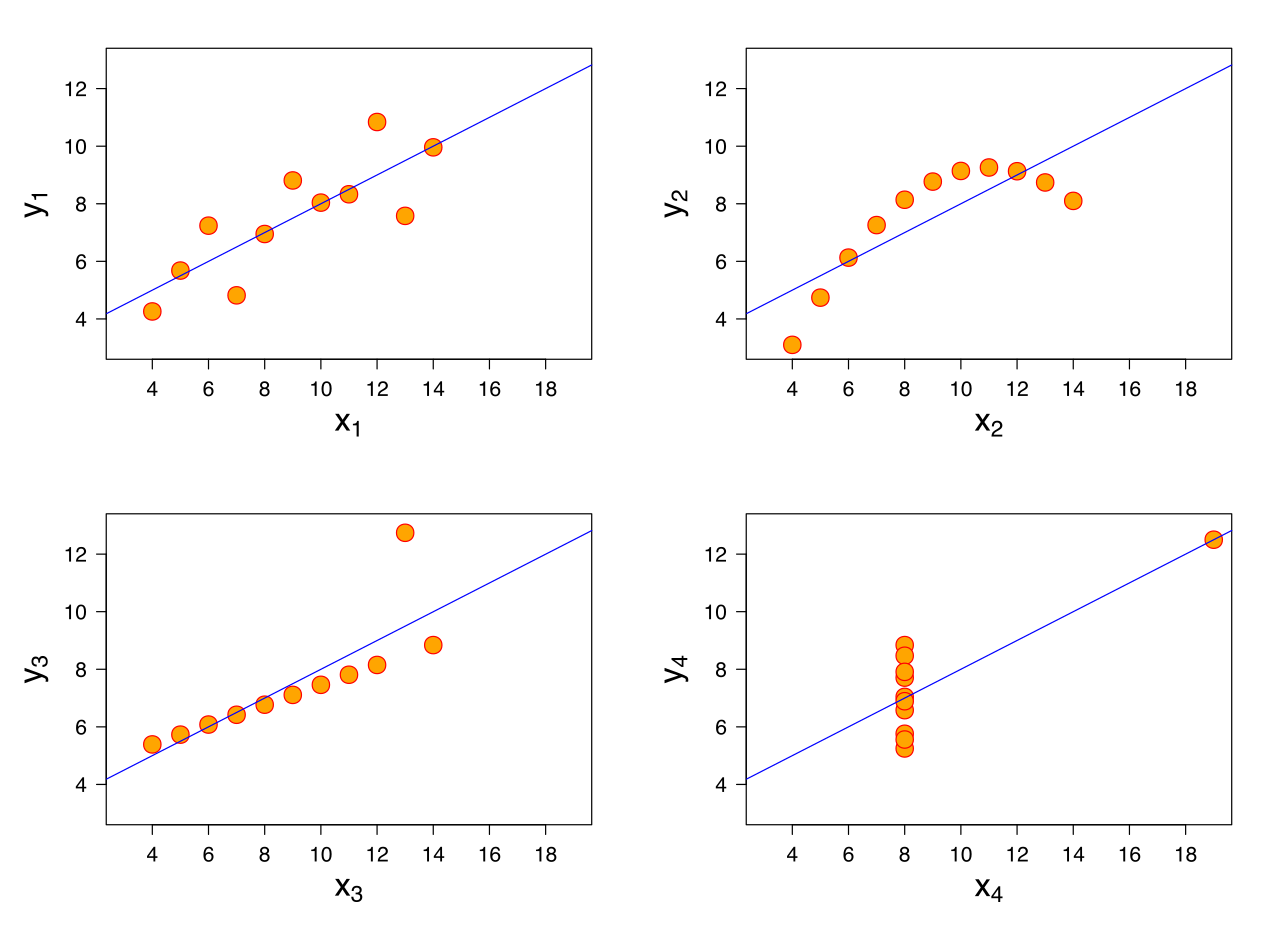
\includegraphics[width=0.9\textwidth,valign=t]{tex/introduction/anscombe.png}
\caption[Anscombe's quartet.]{
Plots of the four data sets of Anscombe's quartet\footnotemark. All data sets have the same mean and sample variance for both axes, the same correlation between the axes, and the same regression lines.
}
\label{figs:anscombe}
\end{figure*}
\footnotetext{Image source: Wikipedia}

Visual Analytics is the area of studying interactive graphical respresentations for analyzing complex data such as Anscombe's quartet mentioned above.
This is often done in addition to and with the help of computational and statistical procedures.
Various studies \cite{doi:10.1080/01621459.1984.10478080,Treisman:1985:PPV:5088.5091,Chang:2002:GTV:820060.820062} have been performed to establish visual principles to effectively take advantage of the high processing power of the human visual system.
Additionally, interaction with the graphical representations allows to hide some of the information and reveal it through interaction to not overwhelm the analyst.
For example, ``overview first; details on demand"~\cite{Shneiderman96theeyes} is a popular mantra taking advantage of interaction.

In the context of machine learning, visual analytics, at first, seems to be a roadblock.
Integrating a human in a machine learning workflow inevitable leads to said human being the bottleneck.
Humans are magnitudes slower than computers which have to idle while waiting for human input.
Thus, human input should only be required for tasks that are impossible without.

For example, with the goal of improving the accuracy of a model a human should not have the task of, \eg, manually picking the order of the features to be included in a decision tree.
A good intuition might outperform the computer momentarily but having an objective goal makes it possible to eventually find a suitable algorithm that is en par or even outperforms the human.
Additionally, manual decisions are not generalizable to other tasks and not scalable to larger datasets which in turn is the reason to use machine learning to begin with.

However, humans have \emph{soft-knowledge}.
That is, they have a general understanding of the world that is typically not codified for machines in all details.
Machines can only work with the data they have.
Their data is their \emph{universe} and to them nothing else exists.
Thus, only humans have the potential to detect and correct when machine learning models acquire incorrect assumptions about their environment.
Visual Analytics can help debugging models, as well as, its data.

Additionally, Visual Analytics can help humans, especially domain experts for a problem that is to be solved using machine learning, to verify the \emph{semantic accuracy} of a model.
That is, whether decisions made by the model ``make sense".
Often, the root cause of semantically inaccurate models is due to biased data.
Thus, statistical accuracy (\ie, the proportion of correctly predicted instances) of a model can be higher than of a different model, while simultaneously being semantically less accurate (see \cite{Caruana:2015:IMH:2783258.2788613,explainer}).

Finally, as humans use machine learning models to speed up and improve decision making, human users need to be able to trust the decisions made by the model.
Visual Analytics can help with \emph{understanding} the decision's made by machine learning models and therefore improve the \emph{trust} in the correctness of those decisions.

\section{Use Case: Machine Learning for Health Care}
In this thesis we will mostly explore use cases from the medical domain\footnote{However, results are easily transferable to other domains as well.}.
It is quite interesting to see parallels between the decision making process of doctors and machine learning.

Over thousands of years the health care domain has evolved into what we now know as evidence based medicine.
That is, new drugs can only be approved after long studies that show significant improvements and methods have been developed and refined over time to improve their measurable effectiveness.

For example, when a patient is examined by a doctor, the doctor follows a structured approach similar to a decision tree.
The first few nodes in the tree set up the context: age, ethnicity, weight, visual appearance, \etc.
A young patient has a vastly different set of potential health risks than an old patient.
Likewise, a physically active patient has different health risks than an obese patient.
Only after those initial features come symptoms into play.
This pattern is also reflected in the documentation of a patient encounter, the doctor's note.
Doctor's notes are structured in a way that reinforces this decision tree approach by putting the context establishing features first.

When it comes to symptoms, doctors often have to weigh different plausible diagnoses against each other, as the same symptoms can appear from different causes.
This is called \emph{differential diagnosis}.
In order to determine which diagnosis has the highest likelihood, Bayesian reasoning is applied~\cite{mdbook}.
That is, the conditional probabilities of symptoms with respect to different diagnoses are compared to each other.
The probabilities are determined through historical records.
However, the resulting rules are often simplified to be memorizable by humans.

While residents (recent medical doctorate graduates) follow those rules religiously, attending physicians (more senior medical doctors) might sometimes follow their intuition, acquired through years of patient interactions.
Thus, such a medical decision might not be fully explainable through empirical statistics alone anymore.
This is equivalent to, for example, a Deep Neural Network that learned some transformations through its hidden layers that lead to hard to interpret interactions of the initial input features.

\section{Motivation}
\todo{Motivation}
Modern machine learning algorithms have reached a degree of potential that lets the resulting models model almost any dataset.
But even though there are statistical measures to guarantee that the model is learning correctly without over fitting on the training data, the model with the highest accuracy is not always the most usable model or even semantically correct.
The following three examples aim to showcase this:

\par \noindent (1)
\todo{pneumonia example}
% \cite{Caruana:2015:IMH:2783258.2788613}

\begin{figure}
\centering
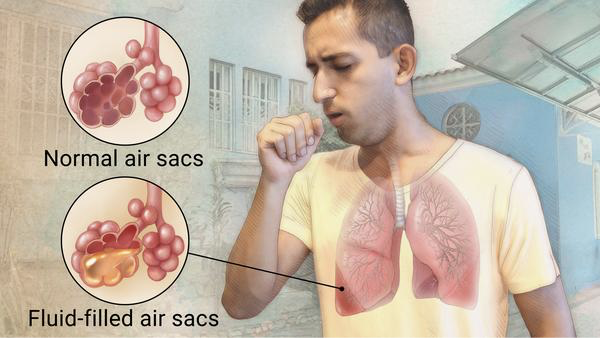
\includegraphics[height=6em,valign=t]{tex/introduction/pneumonia.png}
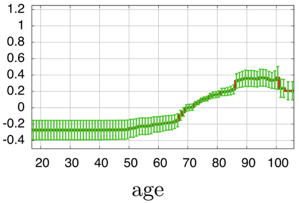
\includegraphics[height=8em,valign=t]{tex/introduction/age.png}
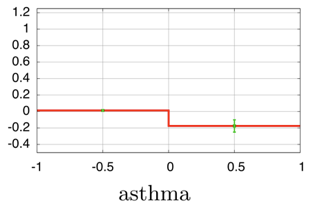
\includegraphics[height=8em,valign=t]{tex/introduction/asthma.png}
\caption{
\todo{TODO}
}
\label{figs:pneumonia}
\end{figure}

\par \noindent (2)
\todo{radio example}
% \cite{Bird:2002:ERI:1251972.1252349}
% https://people.duke.edu/~ng46/topics/evolved-radio.pdf

\begin{figure}
\centering
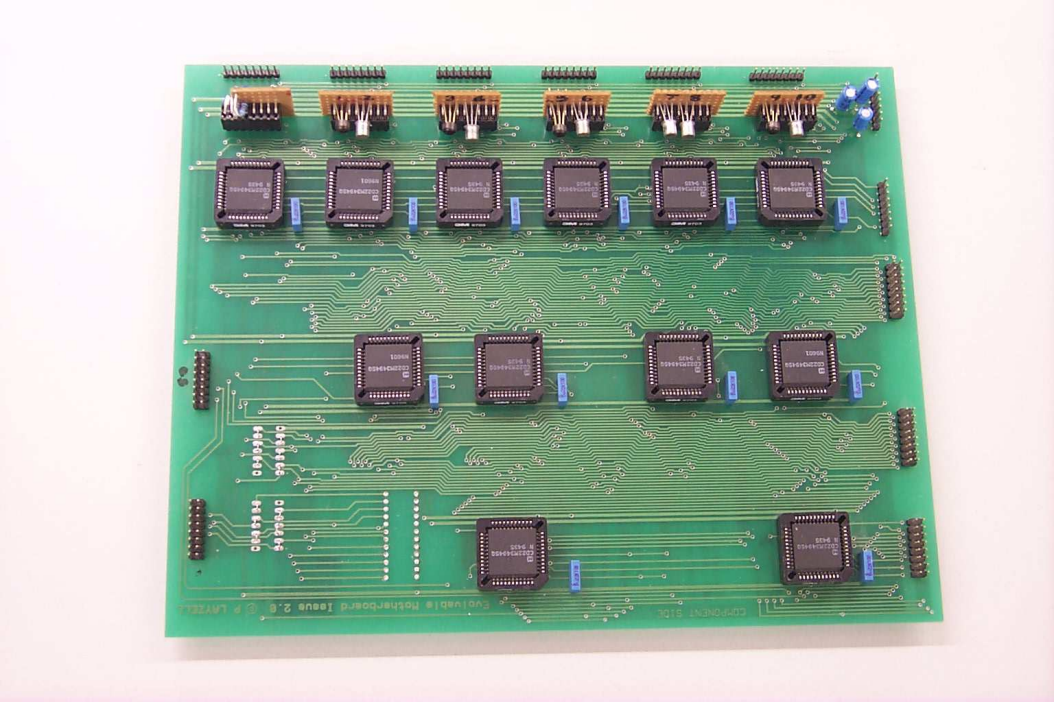
\includegraphics[height=10em]{tex/introduction/emradio.png}
\caption{
\todo{TODO}
}
\label{figs:emradio}
\end{figure}

\par \noindent (3)
\todo{toaster example}
% \cite{2017arXiv171209665B}
% https://arxiv.org/pdf/1712.09665.pdf

\begin{figure}
\centering
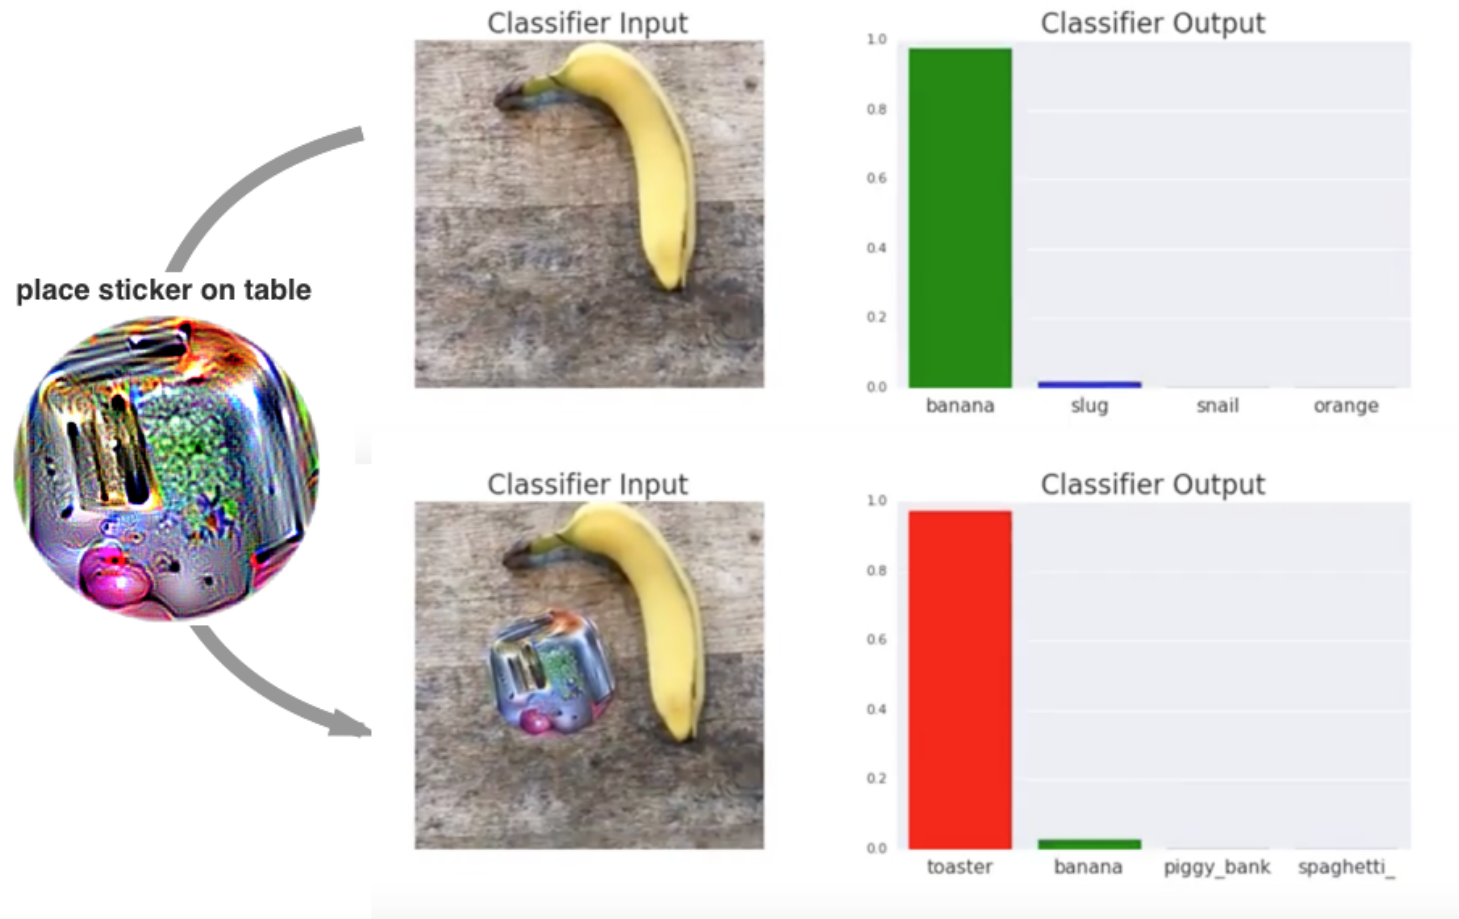
\includegraphics[height=10em]{tex/introduction/adversarialtoaster.png}
\caption{
\todo{TODO}
}
\label{figs:toaster}
\end{figure}

Those three examples all exhibit limitations of machine learning models where increasing the statistical accuracy of the model does not result in a semantically more correct model.
This is due to inherent biases of the data.

In the pneumonia example (1) patients with exceptionally high mortality risk were removed from the data leading to the model being unable to detect the severity of those cases.
In the radio example (2) the model utilized contextual data from the environment that is present but \emph{should} not be used in the model.
And in the toaster example (3) the model expected that all input data is coming from physical, real, objects.
Those biases cannot be detected from within the model or the data itself.
Furthermore, the process of detecting those errors, or even optimizing for semantic accuracy cannot be automated or be formulated as procedure, since there is no objective or measurable optimization criteria for it.
This is in contrast to statistical accuracy where a higher number always indicates a better model.
As a result, human judgment and contextual knowledge is absolutely necessary.

% There has been research...specialized models
In order for a technique to be effectively useful for a human it needs to have few restrictions \todo{}
* reasons for black box
\todo{problem statement}
\section{Research Overview and Thesis Contributions}
\label{sec:corecontributions}
The main goal of this thesis is to explore how model agnostic feature contribution methods can help to gain a holistic understanding of, as well as, insights about predictive models using visual analytics. In three stages, we will show the progression from initial observations, that led us to utilizing black-box analysis, to the eventual use of aggregated instance-level explanations to understand, trust, and verify predictive models. Additionally, we show that our developed visual analytics techniques can be helpful for feature engineering.

Feature engineering is the task of deciding which features will be collected for a particular machine learning problem and how those features are pre-processed or transformed in order to create favorable model results. It requires both expertise of the problem domain, as well as, experience in picking and manipulating features in ``the right way". For the most part, feature engineering cannot be automated and is typically seen as ``black-art" as it relies on intuition and creativity of the modeler \cite{Domingos:2012:FUT:2347736.2347755}.

\subsection{\emph{\infuse}}
In the first stage, we analyze and compare different feature selection strategies. Feature selection is a pre-processing step that, unlike feature engineering, algorithmically determines the possible predictive impact of a feature. Only the most impactful features are then used as input for the predictive modeling process. This is often necessary as a larger number of features require significantly more training examples to accurately represent the valid input space without losing predictive qualities. As feature selection algorithms use similar statistical tools as many predictive modeling techniques it seems plausible to infer the importance of features in the context of decision making through feature selection in a model agnostic way.

Being able to visually compare different feature selection strategies the machine learning experts noticed that, depending on the chosen feature selection algorithm, different, mostly distinctive, feature sets were deemed to be important while, at the same time, having no significant impact on predictive performance. Additionally, from the view of a domain expert those feature sets were equally reasonable in the context of the prediction task.
This demonstrates that \textbf{inspecting} and \textbf{comparing alternate settings} lets machine learning experts develop insights that \textbf{overwrite} their \textbf{initial intuitions}.
Also, concluding that rankings from feature selection algorithms are not informative enough to provide the importance of features in the context of understanding model decisions, a more powerful model agnostic approach is needed.

\subsection{\emph{\prospector}}
In the second stage, we explore the influence of features in the decision making process of predictive models through a technique called partial dependence. Partial dependence computes feature impact on model outcomes by systematically probing the model with artificial inputs. That is, while keeping the rest of the input values the same, the inspected feature assumes all possible values showing the relationship of feature values to the prediction score. Aggregated over all observed instances, the general behavior of the model with respect to a given feature can be inferred. By computing a novel feature importance score from partial dependence relationships unusual and interesting relations can be found quickly without having to inspect all, often several thousand, features.

Analyzing partial dependency relationships on diabetes prediction models trained on electronic medical records containing patient demographics, diagnoses, medications, and laboratory results, using our method we gained several insights. Firstly, we showed that logistic regression models are not expressive enough to accurately model the complex relationships of certain features to the outcome. Secondly, imputation of missing values, using the population average in laboratory results, caused the model to become uncertain close to the normal value range of laboratory tests. Lastly, we found that the model used a proxy variable indicating the number of doctor visits as predictor of the healthiness of a patient.
However, this is \emph{not} a valid predictor.
Even though a patient is likely to visit a doctor more often if she is sick, the reverse cannot be said. The above findings show how \textbf{partial dependence} with the proposed \textbf{feature importance score} allow analysts to effectively \textbf{detect model errors} related to \textbf{over-} and \textbf{under-fitting}, \textbf{imputation}, and \textbf{leaking labels} caused by incorrect cause-effect relationships.
However, a major drawback of using partial dependency is its limitations on extending it to relations of multiple features to the predicted outcome.

\begin{figure}[t]
\centering
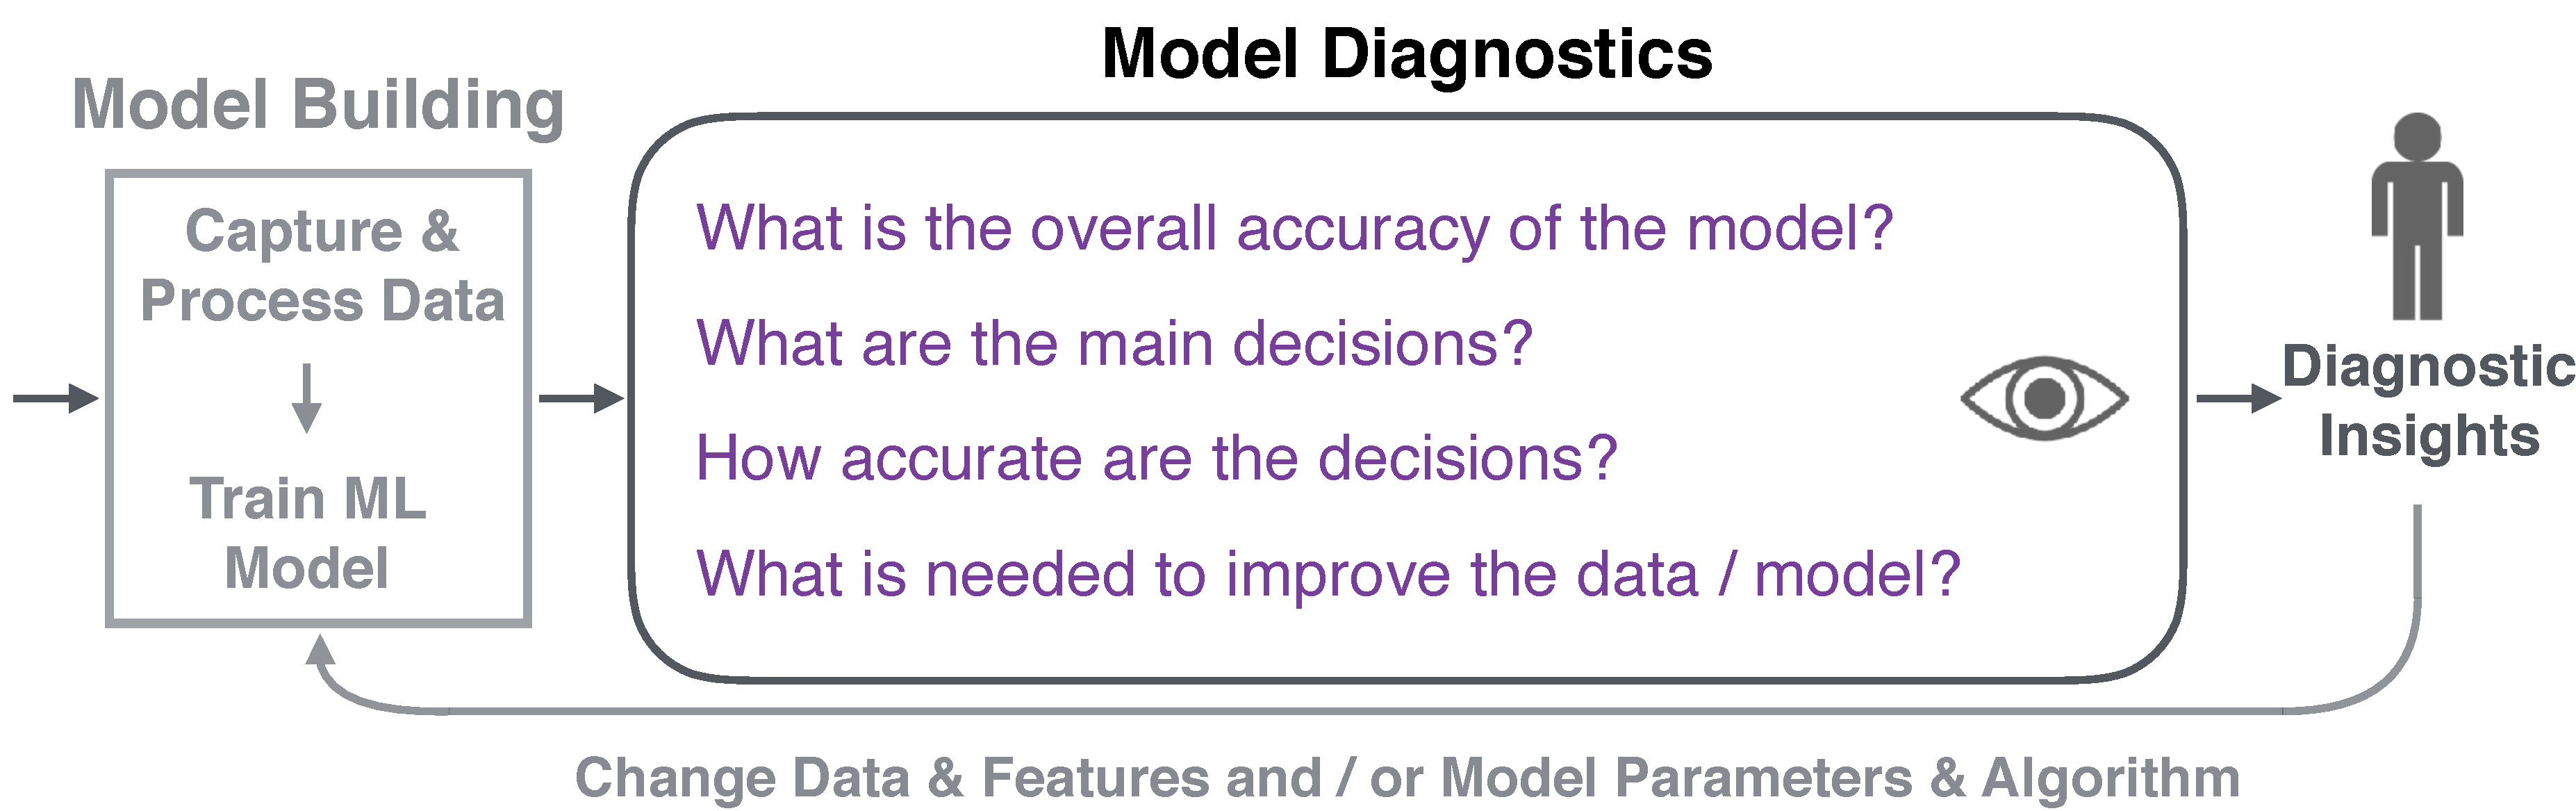
\includegraphics[width=\textwidth]{figs/workflow_large}
\caption[The model diagnostic workflow.]{
The proposed \textit{model diagnostic} workflow extends the conventional \textit{model building} workflow in machine learning for enabling domain experts to reason about the semantic validity of the decisions made by any model through multiple linked visualizations.
This ultimately helps to improve data acquisition and model generation processes belonging to the original workflow.
}
\label{figs:workflow_intro}
\end{figure}

\subsection{Model Diagnostic Workflow}
In the third stage, we overcome those limitations by leveraging instance-level explanations. Instance-level explanations are defined as the smallest change, to an instance vector, necessary to change the predicted outcome label. Aggregating over those explanations and statistically analyzing the resulting instance subsets, proves as powerful novel approach for understanding the behavior of a model. Additionally, we propose a Model Diagnostic workflow (see \figref{figs:workflow_intro}) that helps identify flaws in the \emph{input data}, used to train and test the model.

\begin{table}[t]
     \begin{tabular}{l|c|c|c} 
     \textbf{Approach} & \makebox[0pt][l]{\textbf{Instances}}\phantom{Aggregated} & \textbf{Aggregated} & \makebox[0pt][l]{\textbf{Global}}\phantom{Aggregated} \\ 
     \hline
     \hline
     \infuse & & & X \Tstrut\\
     \hline
     \prospector & X & & X \Tstrut\\
     \hline
     \textit{Model Diagnostic workflow} & & X & \Tstrut\\
    \end{tabular}
    \centering
    \caption[Locality of decision analyses of the presented approaches.]{Locality of decision analyses of the presented approaches. \textbf{Instances} refers to analyzing decisions for one instance at a time. \textbf{Aggregated} refers to analyzing decisions for groups of instances and \textbf{Global} refers to analyzing decisions globally without inspecting decisions for individual instances.}
    \label{tab:locality}
\end{table}

We use this workflow to analyze a predictive modeling problem revolving around patient admission to a hospital, of patients in the emergency department of said hospital. Accurately predicting whether a patient eventually gets admitted to the hospital helps reducing costs. The major limiting factor of this prediction task is the need for input features readily, and electronically, available at the earliest point possible. To this extend we initially used features of prescribed medications as this information is immediately available electronically. Our analysis showed that there are clear groups of patients where the predictive model is very helpful. However, there are some groups of patients where it is impossible for the predictive model to make accurate predictions given the provided information. One of those groups is patients receiving Diatrizoate Meglumine, a contrast medium for CAT or PET scans. This medication only indicates that a scan was performed, but does not carry information about the result of the scan. However, the result of the scan is the deciding factor whether a patient needs further care or can get sent home. Thus, with the given information it is impossible for the predictive model to make a decision that performs better than random guessing. Including more information in the form of additional features does indeed help with this problem but pushes the time when a decision can be made further back. One possible solution is to utilize the predictive model only for the confident groups of patients and wait for the doctors' decisions in other cases. This example illustrates that it is not only possible to \textbf{understand decision making} of a predictive model through the \textbf{Model Diagnostic workflow} based on \textbf{aggregated instance-level explanations}, but also how it can be applied for \textbf{semantic validation} and \textbf{feature engineering} on the input data.

\subsection{User Study on Aggregating Explanations}
In order to show the generalizability of the Model Diagnostic Workflow we conducted a user study to explore the effectiveness of aggregated instance-level explanations in detecting biases in the input data.

First, we generalized aggregating instance-level explanations to numerical input data.
We achieved this by using histograms of the input features, similar to \cite{seekaview}, ordered by the features' aggregated importance.
Furthermore, we allowed the comparison of selected, meaningful, subsets to each other.
Then, we compared this aggregated representation, in a user study, to the commonly used approach of individually inspecting instance-level explanations one-by-one using a tabular representation.

We found that aggregating instance-level explanations, with our method, significantly \textbf{outperforms} inspecting \textbf{individual explanations} in its ability to enable detection of biases in the data.
However, our method \textbf{requires explanations} in order to perform correctly.
Additionally, we found that instance-level explanations \textbf{hurt} bias detection performance for a \textbf{tabular representation}.
We hypothesize that the added difficulty of inspecting a table without the help of explanations forces users to \textbf{interact} more strongly with the user interface, thus providing better results.
This is a known effect (see Hullman~\etal~\cite{6064986}).

All in all, aggregating instance-level explanations perform as well as explanation-free tabular representations, which require high user engagement.
Additionally, our method promises a higher scalability due to its independence from the total number of instances.

Furthermore, we could reproduce findings from Stumpf~\etal~\cite{harmful}, claiming that instance-level explanations might make users over-confident in their understanding of a model.
However, we also showed that aggregated instance-level explanations overcome this problem.

% In addition to those promising results, there is still work to do.
% It still needs to be shown that the proposed workflow of statistical analysis of instance-level explanations can be successfully applied to other data types than binary feature vectors, such as numerical features or highly redundant features such as found in images.
% Early results in this direction indicate that it might be beneficial to abandon the focus on features to explain machine learning models, but rather focus on instances directly.
% That is using instance-level explanations to obtain groups of \emph{instances} with similar behavior and then visualize those groups (\eg, using techniques proposed by \cite{seekaview}) in order to \emph{implicitly} explain them.
% This provides more flexible explanations than those proposed earlier as their capability goes beyond ``Feature A and feature B positively impact the prediction for this group of instances" to also allow insights of the form ``The number of circles formed by black pixels contribute positively to the prediction" which would be very difficult to formulate by a machine but are easily formulated by humans using visualizations.
% Furthermore, we are going to run a study on the implications on confidence in and trust of machine learning models when using different explanation approaches.
% \todo{END?}
\section{Thesis Outline}
\label{sec:thesisoutline}
We organize the remainder of this thesis in the following manner.
In \chapref{chap:infuse} we will describe and discuss the \infuse system for comparing different feature selection strategies.
In \chapref{chap:prospector} we will describe and discuss the \prospector system for inspecting models via partial dependence plots.
Following, we will introduce the \emph{Model Diagnostic workflow}, aggregating instance-level explanations, in \chapref{chap:explainer} and discuss its capabilities in the context of binary input data.
Afterwards, in \chapref{chap:aggexplain} we will extend this workflow to numerical input data and explore its effectiveness compared to individually inspected instance-level explanations.
In \chapref{chap:summary}, we present a summary of the work while discussing key findings, implications, and open issues, leading to further research opportunities for future researchers.
Finally, in \chapref{chap:future_work}, we discuss the conclusions and future work.
\chapter{INFUSE}
\label{chap:infuse}
%!TEX program = xelatex

% \documentclass[journal]{vgtc}                % final (journal style)
% \documentclass[review,journal]{vgtc}         % review (journal style)
%\documentclass[widereview]{vgtc}             % wide-spaced review
%\documentclass[preprint,journal]{vgtc}       % preprint (journal style)
%\documentclass[electronic,journal]{vgtc}     % electronic version, journal

% \usepackage{mathptmx}
% \usepackage{graphicx}
% \usepackage{times}
% \usepackage{subfigure}
% \usepackage{amsmath}
% \usepackage[usenames,dvipsnames]{xcolor}
% \usepackage{tikz}
% % \input{tex/packages}
% \usepackage[bookmarks,backref=section,linkcolor=black]{hyperref} %,colorlinks
% \hypersetup{
%   pdfauthor = {},
%   pdftitle = {},
%   pdfsubject = {},
%   pdfkeywords = {},
%   colorlinks=true,
%   linkcolor= black,
%   citecolor= black,
%   pageanchor=true,
%   urlcolor = black,
%   plainpages = false,
%   linktocpage
% }
% \usepackage[numbers,square]{natbib}
% \usepackage{doi}
% \usepackage{url}

%\newcommand{\enrico}[1]{\textcolor{NavyBlue}{[#1]}}
%\newcommand{\joschi}[1]{\textcolor{JungleGreen}{[#1]}}
%\newcommand{\adam}[1]{\textcolor{RedOrange}{[#1]}}

% \onlineid{0}
% \vgtccategory{Research}
% \vgtcinsertpkg

% \title{INFUSE: Interactive Feature Selection for Predictive Modeling of High Dimensional Data}
% \author{Josua Krause, Adam Perer, Enrico Bertini}
% \authorfooter{
% %% insert punctuation at end of each item
% \item
%  Josua Krause is with NYU Polytechnic School of Engineering. E-mail: jk4560@nyu.edu.
% \item
%  Adam Perer is with IBM T.J. Watson Research Center. E-mail: adam.perer@us.ibm.com.
% \item
%  Enrico Bertini is with NYU Polytechnic School of Engineering. E-mail: enrico.bertini@nyu.edu.
% }

% \shortauthortitle{Krause \MakeLowercase{\textit{et al.}}: }

\begin{quote}
\textit{Predictive modeling techniques are increasingly being used by
data scientists to understand the probability of predicted outcomes.
However, for data that is high-dimensional, a critical step in predictive
modeling is determining which features should be included in the models.
Feature selection algorithms are often used to
remove non-informative features from models.
However, there are many different classes of feature selection algorithms.
Deciding which one to use is problematic as the algorithmic output
is often not amenable to user interpretation.
This limits the ability for users to utilize their
domain expertise during the modeling process.
To improve on this limitation, we developed \infuse ,
a novel visual analytics system designed to help analysts
understand how predictive features are being ranked across
feature selection algorithms, cross-validation folds, and classifiers.
We demonstrate how our system can lead to important insights
in a case study involving clinical researchers predicting patient
outcomes from electronic medical records.
}\end{quote}

\begin{contributions}{Foo}
\item \todo{TODO}
\end{contributions}

\begin{quote}
\textit{Josua Krause, Adam Perer, Enrico Bertini}
\end{quote}

% \keywords{Predictive modeling, feature selection,
% classification, visual analytics, high-dimensional data}
% %% ACM Computing Classification System (CCS).
% %% See <http://www.acm.org/class/1998/> for details.
% %% The ``\CCScat'' command takes four arguments.

% \CCScatlist{ % not used in journal version
%  \CCScat{K.6.1}{Management of Computing and Information Systems}%
% {Project and People Management}{Life Cycle};
%  \CCScat{K.7.m}{The Computing Profession}{Miscellaneous}{Ethics}
% }

% Uncomment below to include a teaser figure.


\begin{figure*}
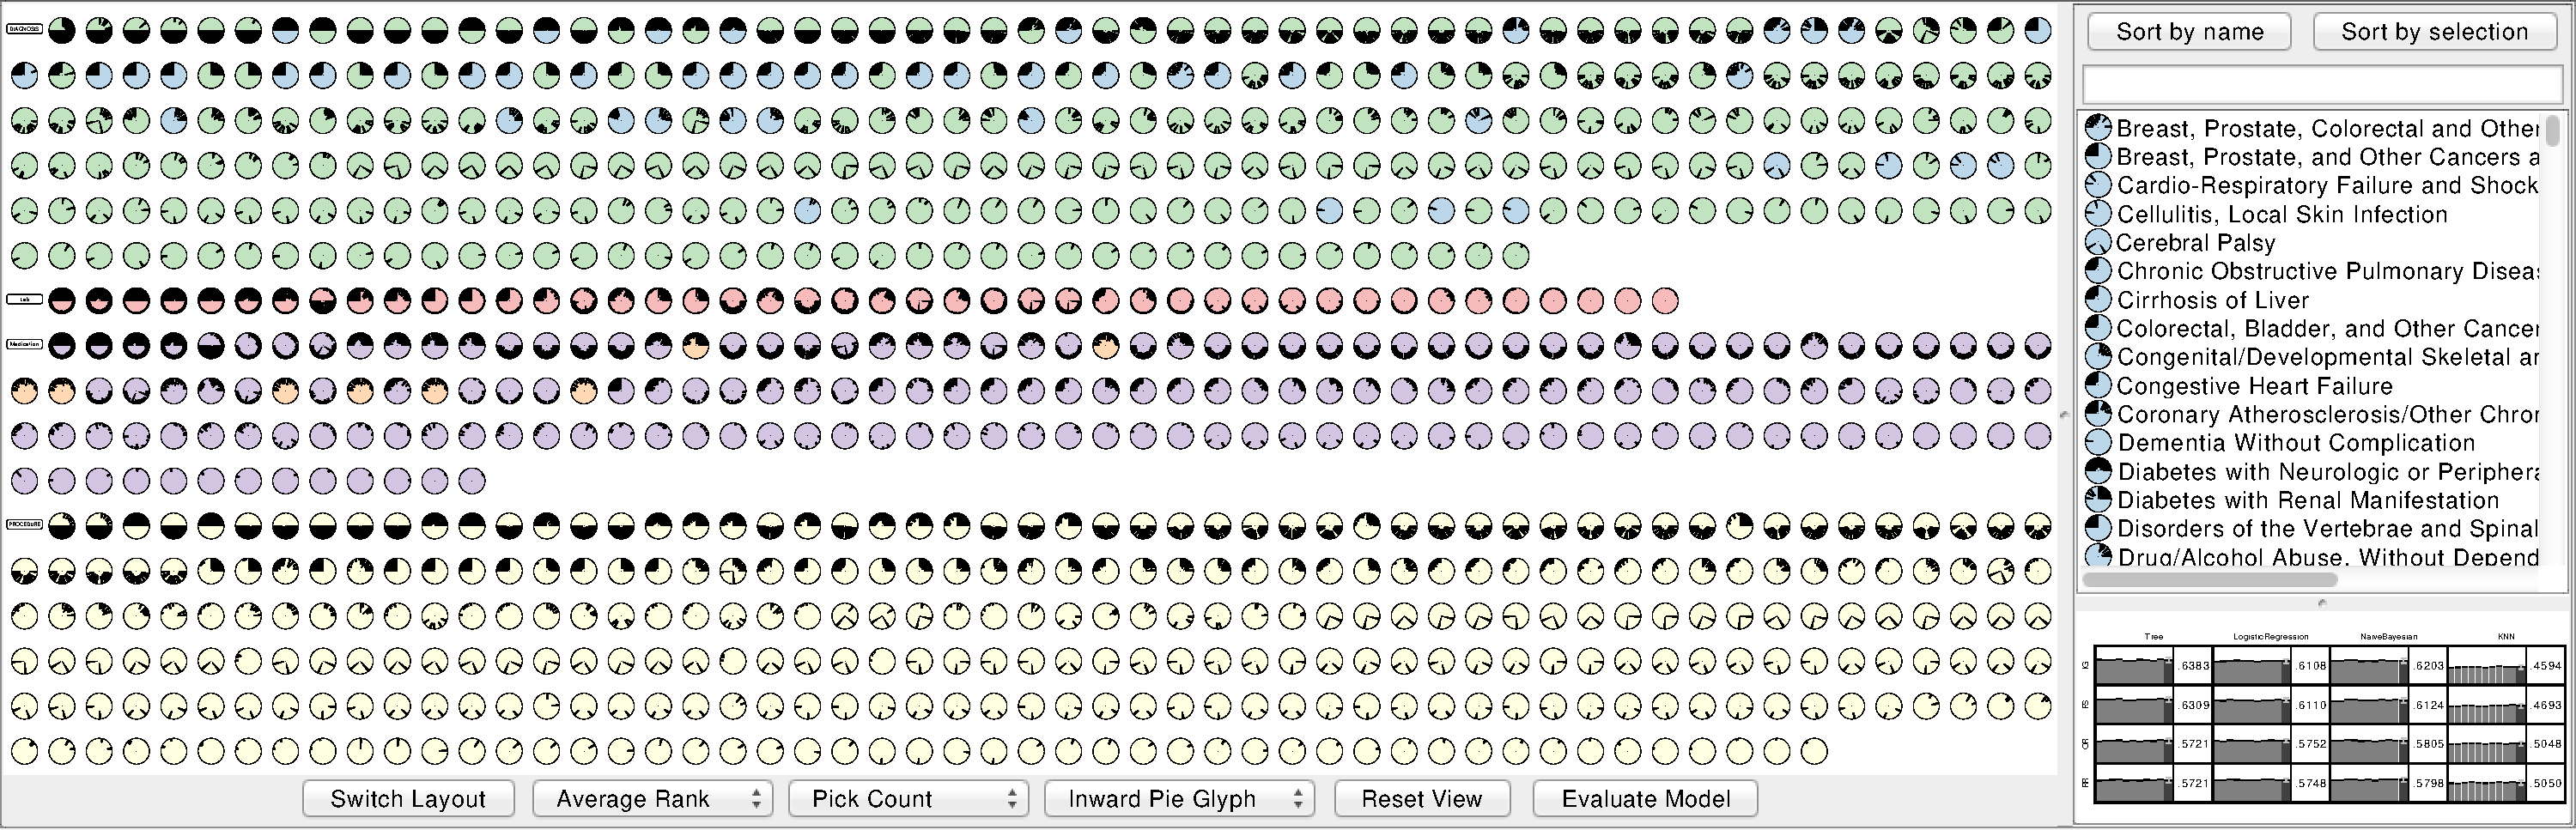
\includegraphics[width=0.95\textwidth]{infuse/teaser}
\caption{
An overview of \infuse, a visual analytics tool that supports users to understand the predictive power of features in their models.  Each feature is ranked by various feature selection algorithms, and the ranking information is visualized in each of the three views within the system.  On the left, the Feature View provides a way to visualize an overview of all features according to their rank using a variety of layouts.  On the top-right, the List View provides a sorted list of all features, useful for selections.  On the bottom-right, the Classifier View provides access to the quality scores of each model.  Each of the views are coordinated, and users can brush between all three views.
}
\label{fig:teaser}
\end{figure*}

%% Uncomment below to disable the manuscript note
%\renewcommand{\manuscriptnotetxt}{}

%% Copyright space is enabled by default as required by guidelines.
%% It is disabled by the 'review' option or via the following command:
% \nocopyrightspace

% \begin{document}
\section{Introduction}

% \maketitle

% !TEX root = ../featureselection.tex
\begin{figure*}[ht]
\centering
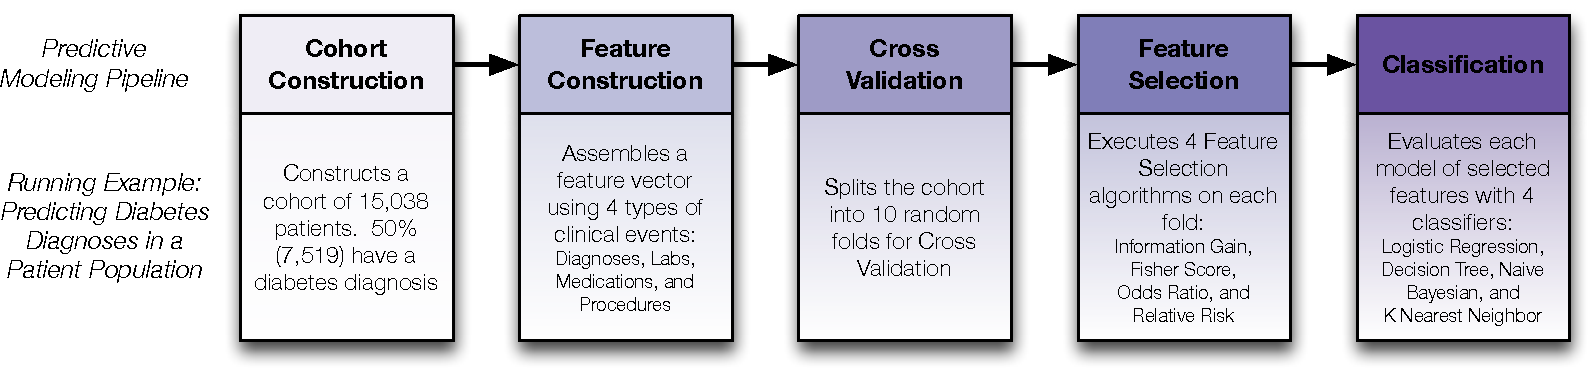
\includegraphics[width=\linewidth]{infuse/pipeline}
\caption{Steps of a typical predictive modeling pipeline.  For each step, we provide the details of the running example we use throughout the paper.
}
\label{fig:pipeline}
\end{figure*}

The visualization research community has usually focused on developing techniques and systems to support the analysis of datasets, with limited analysis of the relationship between datasets and the construction of models on top of them. However, there are a growing number of data scientists interested in more than just interpreting their data: they want to understand their data and predictive probabilities associated with them. Providing visual support for this kind of task has become important as many existing applications on the market and in scientific settings need to solve problems that are predictive in nature, e.g. prediction of customer behavior, diseases, drug effectiveness.

Predictive modeling is defined as the process of developing a mathematical tool or model that generates an accurate prediction \cite{kuhn2013applied}. However, building an accurate predictive model is far from trivial. First, modelers must construct cohorts, or distinct groups, to divide their datasets into cases and controls. Then, they must use a feature construction technique to define the feature vector. Next, they must define the parameters for cross-validation to ensure the results are statistically valid and robust. Then, they need to choose a feature selection algorithm to extract the informative features and include them in a model. And finally, they need to choose a classifier to evaluate the predictiveness of the model. For each of these decisions, there are a variety of techniques for cohort construction, feature construction, cross-validation, features selection, and classification to choose from, and there are currently no systematic guidelines to decide which algorithms are most appropriate for which types of datasets. Making the wrong choices can cause predictive models to fail. Kuhn and John argue that many predictive models fail because, ``predictive modelers often only explore relatively few models when searching for predictive relationships [...] due to either modeler's preference for, or knowledge of, or expertise in, only a few models or the lack of available software that would enable them to explore a wide range of techniques" \cite{kuhn2013applied}. We use these current limitations as motivation to research how visual analytics may improve the process of predictive modeling.

Our proposed research focuses on an important step in the predictive modeling pipeline: feature selection. When data is high-dimensional, feature selection algorithms are often used to remove non-informative features from models. Again, the analyst is confronted with the decision of which feature selection algorithm to utilize, and even if the analyst decides to try out multiple types, the algorithmic output is often not amenable to user interpretation. This limits the ability for users to utilize their domain expertise during the modeling process. To improve on this limitation, we developed \infuse (INteractive FeatUre SElection), a novel visual analytics system designed to help analysts understand how predictive features are being ranked across feature selection algorithms, cross-validation folds, and classifiers. We describe the tasks associated to the feature selection and understanding process and provide a design rationale for our solution. We also demonstrate, through case studies, how the system can lead to important insights for clinical researchers predicting patient outcomes from electronic medical records.

Concretely, our contributions include:

\begin{itemize}
\item A design and implementation of a predictive modeling exploration system,
\infuse, for understanding how predictive features are being ranked
across feature selection algorithms, cross-validation folds, and classifiers.
\item An Interactive Model Builder, where users can create customized models based on insights reached with \infuse, and then have their results evaluated in comparison to automated methods.
\item A case study of domain experts using
\infuse  to explore predictive models in electronic health records.
\end{itemize}

% The following text is taken from the PARAMO paper:
% "To develop an accurate and useful predictive model, a research- er generally needs to build and compare many different models as part of the discovery workflow. Each model can be viewed as an instance of the modeling pipeline and consists of a unique combination of the data, algorithms, and/or certain parameter configurations in the task components.
% A number of factors combine to increase the number of models that need to be explored, resulting in a large set of pipelines that have to be processed. First, the volume, variability, and heteroge- neity of EHR data require significant processing in building predic- tive models [10]. Second, there is uncertainty in knowing a priori which feature construction, feature selection, and classification algorithms are most appropriate for the specific target application [27]. As such, composition of an appropriate predictive model re- quires exploring a potentially large space of possible algorithms and parameters and their combinations. Third, for some biomedi- cal applications, the ability to interpret how the model works is just as, if not more, important than the accuracy of the model. Here, it is important to explore a variety of classification algo- rithms (e.g. decision trees, Bayesian networks, and generalized regression models) that produce trained models which can be interpreted by domain experts to verify and validate that the mod- el is clinically meaningful [28]. It is likely that multiple models can have similar performance in terms of prediction accuracy, but may differ significantly in their internal model parameters. By building multiple models, it becomes possible to select ones that have more clinically meaningful interpretations. Fourth, it is critical to statis- tically validate the models to ensure generalizability and accuracy. Cross-validation techniques can help with this endeavor, but can dramatically increase the number of models that need to be built and evaluated.""

\begin{figure*}[ht]
\centering
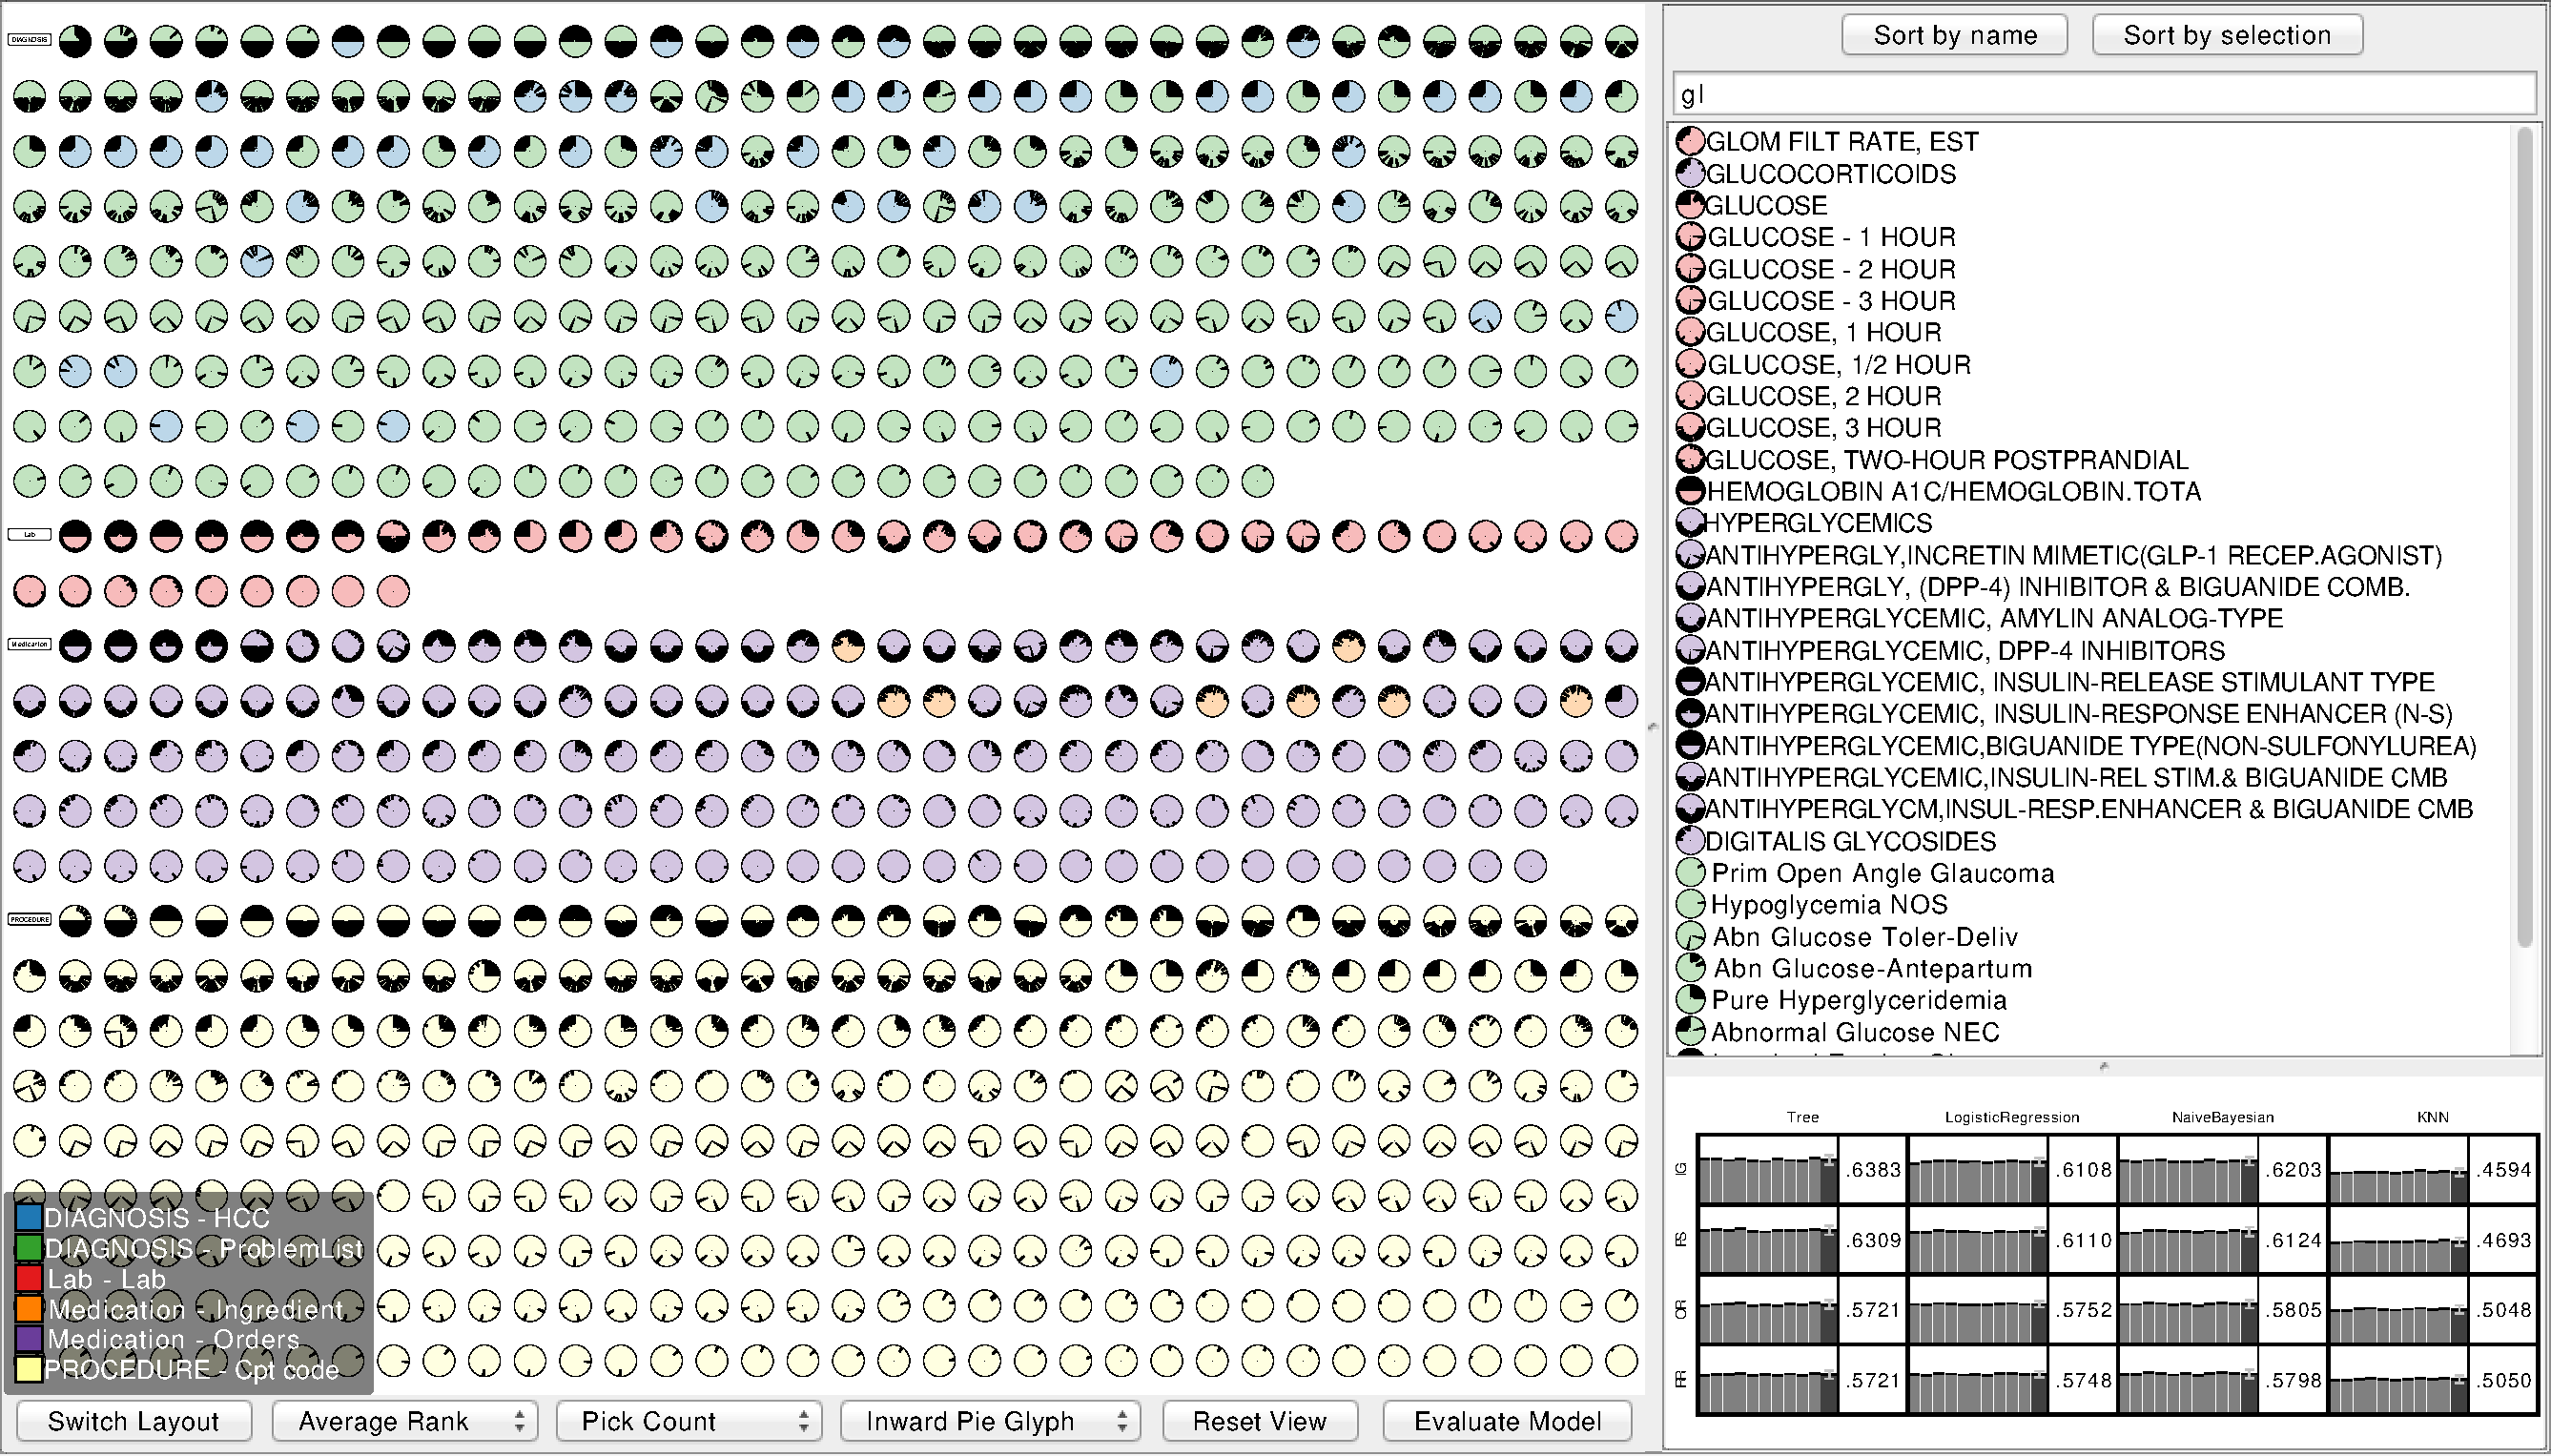
\includegraphics[width=\linewidth]{infuse/system}
\caption{
An overview of \infuse, a system for interactive feature selection.  On the left, the Feature View provides a way to visualize an overview of all features grouped by type and then sorted by importance.  The color key for the feature types and subtypes are shown at the bottom.  The buttons and combo boxes at the bottom can be used to switch layouts and define the axes of the scatterplot view shown in
Figure~\ref{fig:scatter}.  On the top-right, the List View provides a sorted list of all features, useful for selections.
This list can be filtered using the search box above. Currently only features containing the term ``gl" are shown.
The remaining features are sorted by the number and position
of the search term occurrences.
On the bottom-right, the Classifier View (Figure~\ref{fig:classifier}) provides access to the quality scores of each model.  Users can also select features and build custom models with the Interactive Model Builder.
}
\label{fig:system}
\end{figure*}

% !TEX root = ../featureselection.tex

\section{Motivation}

\subsection{Predictive Modeling in Health Care}
\label{sec:motivation_healthcare}
Predictive modeling is a common and important methodology used
in medical informatics and health care research.
For instance, it can be used to detect diseases in patients early
before they progress \cite{bellazzi2008predictive} and to
personalize treatment guidelines to understand which populations
will benefit from an intervention \cite{jensen2012mining}.
In order to derive such insights and build successful predictive models,
it is common for health care researchers to implement, evaluate,
and compare many models with different parameters and algorithms.
A common workflow for predictive models is a 5-step process,
illustrated in Figure~\ref{fig:pipeline}:
(1) cohort construction, (2) feature construction, (3) cross-validation,
(4) feature selection, and (5) classification.
There are currently few tools that support this complex
workflow for predictive modelers.

A recent platform, PARAllel predictive MOdeling (\textit{PARAMO}) \cite{paramo},
enables users to specify a small number of high-level parameters
to support this 5-step workflow.
\textit{PARAMO} then uses Map-Reduce to execute these many tasks in parallel.
After the models have been constructed and evaluated by classifiers,
users can compare area under curve (AUC) scores of different models and select the
ones with the highest predictive power.
While this ability to construct and evaluate models at scale is
an important breakthrough for clinical researchers, the clinical
experts are still left out of the loop at each of these 5 stages,
as each of the algorithms act as a black box.

This type of workflow limits the ability of clinical researchers to use
their domain knowledge to assist in the model building phase.
While multiple models may have similar performance in terms of
prediction accuracy, there is a desire to ensure that models
with more clinically meaningful features are selected
\cite{chen2006medical}.

\subsection{Running Example: Diabetes Prediction}
\label{sec:running_example}
In order to make our contributions concrete, we
utilize a running example from our case study.
Our case study involves a team of four clinical researchers interested
in using predictive modeling on a longitudinal database of
electronic medical records. The research team consisted of one MD researcher with a background in emergency medicine, and three PhD researchers with backgrounds in health care analytics.
Their database features over 300,000 patients from a major
health care provider in the United States.
The team is interested in building a predictive model to predict if a patient
is at risk of developing diabetes, a chronic disease of high blood sugar levels
that causes serious health complications.

From this database, the team constructs
a cohort (Step~1) of 15,038 patients.
50\% of these patients (7,519) are considered
incident cases with a diagnosis of diabetes.
Each case was paired with a control patient based on
age, gender, and primary care physician resulting
in 7,519 control patients without diabetes.
From the medical records of these patients,
they extract four meaningful types of features (Step~2): diagnoses,
lab tests, medications, and procedures.
In total, there were 1,627,736 diagnosis events (6,709 unique types), 361,026 lab events (193 types), 818,802 medication events (344 types), and 853,539 procedures (4,403 types).
For our visualization, we only consider types of features that were picked
by feature selection algorithms which results in 859 features to display.

Next, in order to reduce the bias of the predictive models,
the team uses 10 cross-validation folds (i.e. random samples) (Step~3) to divide the
population randomly into 10 groups.
After cohorts, features, and folds are defined, the
clinical researchers are ready to use feature selection.
The team has four feature selection algorithms implemented
and available to them (Step~4): these include \textit{Information Gain}
and \textit{Fisher Score}, which have been used extensively by the researchers,
as well as two new ones which were recently implemented by
their technologists: \textit{Odds Ratio} and \textit{Relative Risk}.
Finally, the team evaluates each selected feature set as a model using
four classifiers (Step~5): \textit{Logistic Regression}, \textit{Decision Trees},
\textit{Naive Bayes}, and \textit{K-Nearest Neighbors}.

Typically, this team executes a pipeline of multiple feature selection
algorithms, and chooses the model that ends up
with the best scores from the classifier.
Although this team has an interest in embedding domain knowledge
into their models, their current platform for running predictive models
does not have a user interface where users can view or edit the
specific features that make up each model.
Therefore, resulting models are typically not interpretable
by domain experts,
and do not support bringing in their medical expertise by prioritizing or removing features that may not be relevant to the disease they are modeling.

\subsection{Task Analysis}
\label{sec:task-analysis}

The data analysis team initially expressed an interest of having a visual analytics system to aid them in making sense of the complex information generated by the modeling pipeline. During our interviews we agreed to focus on the feature selection and classification steps, as they needed visualizations to reason about the effects of choosing different combinations of the available algorithms. Without such visualizations, the researchers ability to choose among different algorithms is ineffective.

Through our interactions with the analysts we derived three main tasks that guided the design of \infuse:


\begin{description}
\item[Task1 - Comparison of feature selection algorithms.] In data sets with thousands of features, it is important to have a quick way to understand how feature selection algorithms rank different features differently. Some of the typical questions the researchers ask are: ``\textit{Which features are consistently ranked highly by all the algorithms?}"; ``\textit{How much do the algorithms differ in their ranking?}"; ``\textit{Are there features that have a high rank with some algorithms and a low rank with some others?}"; ``\textit{How robust are the rankings with respect to different data samples?}"

\item[Task 2 - Comparison of classification algorithms.] The output of each feature selection algorithm is used to feed a series of classification algorithms. At the end of this process, the user is left with a $F \times C$ number of performance comparisons, where $F$ is the number of feature selection algorithms and $C$ the number of classification algorithms. Typical questions our researchers ask are: ``\textit{Which combinations of feature selection and classification algorithms give the best scores?}"; ``\textit{Are there feature selection algorithms that score consistently better across the set of classification algorithms?}"; ``\textit{Are there classification algorithms that score consistently better across the set of feature selection algorithms?}"; ``\textit{Which sets of features are selected in the model(s) that give the highest performance?}"

\item[Task 3 - Manual selection and testing of new feature sets.] Related to the last question of Task 2, the researchers see value in being able to add or remove features of interest from models. This is desired because there can be additional domain-relevant knowledge, beyond model performance, to introduce a desired feature or remove an undesired one.  Typical questions our researchers ask are: ``\textit{How does the performance of the model increase or decrease if I remove or add these features?}"; ``\textit{How does a new model compare to the models automatically built by the system?}"
%;``\textit{How predictive is a single feature?}"
%;``\textit{Could switching to a different lab-test yield similar performance while being less expensive?}".
\end{description}


\infuse was designed to support these three tasks by providing a visualization of large sets of features and how these features are used by the modeling algorithms. After several design iterations, we converged on a visual design where features are first-class citizens of the visual representation: that is, each visual object in the main view represents a feature and its design and layout reflects information obtained from the algorithms.  A representation centered on features aligns well with the analysts' mental model and makes features easily identifiable through their names. Each feature, in fact, represents real-world entities like medications, lab tests and diagnoses, that have rich semantics and can be easily identified and understood by domain experts.

% !TEX root = ../featureselection.tex

\section{Related Work}
While visualization of multidimensional data has traditionally focused
more on the visualization of the data space, visualizing data features
has important applications in real-world scenarios;
especially when confronted with hundreds or even thousands of dimensions.
In this context, visualization helps data analyst making sense of the
feature space while including their background knowledge in the process.
Visual feature selection can, for instance, help rank features according
to predefined scores, detect similarities among dimensions
(thus gauging intrinsic dimensionality of feature spaces),
merge or combine features into composite features.
In the following we review visualization literature that consider
the specific problem of visualizing large sets of features.

\subsection{Visual Feature Selection}
%\enrico{I am wondering if there is a way to structure these techniques into some classes. For instance some are more into finding similarities and groups of dimensions others are more into ranking.}

Several approaches to feature selection and dimensionality reduction, in general, exist in visualization.
The early work of Guo~\cite{Guo2003} introduced the idea of
visualizing relationships between features sets.
His system is based on an interactive matrix view where rows and
columns represent features and the cells are colored according to
feature similarity (calculated as entropy and ${\chi}^2$).
The matrix is automatically sorted to allow selection of subspaces
(feature subsets) where data shows interesting clusters.
Visual hierarchical dimension reduction \cite{wang2003interactive}
allows detection and grouping of similar features as well.
The technique is based on a hierarchical clustering algorithm
which clusters dimensions in terms of their similarity and present
them in a \textit{sunburst} visualization \cite{yang2003interactive}.
Users can interactively choose an aggregation level and use the aggregated
dimensions to display data with the reduced set of dimensions.
Johansson and Johansson \cite{Johansson2009} present an integrated environment based on
\textit{parallel coordinates} visualization where the number and order of
dimensions (axes) presented at any time is guided by a ranking algorithm
that takes into account associations as well as intrinsic interestingness of
each feature to interactively choose how many features to visualize.
Similar in spirit is the \textit{rank-by-feature} framework \cite{seo2005rank} in which
the data features are organized, ranked and visualized in
1D and 2D visual representations
(e.g. histograms, bar charts and scatterplots).
The user can for instance inspect a matrix of feature pairs,
ranked by one of the available ranking functions, and single
out those that show interesting associations.
A similar mechanism is also used in \textit{scagnostics} \cite{wilkinson2005graph} a
quality metric approach \cite{bertini2011quality} that ranks axis pairs according to the pattern/shape they create in a scatterplot visualization.

More similar to the solution presented in this paper are visualizations that
focus on plotting dimensions as data points in the visual representation
(rather than, for example, as axes of a visualization where the data
items represent records of a data table).
\textit{Value and Relation Display} visualizes data features as icons
in a scatter plot visualization \cite{YangPHMWR04}.
The icons are positioned using a \textit{multidimensional scaling}
algorithm which positions dimensions with
similar distributions close together.
The icons are designed to represent the distribution of the
data values within the feature.
Such a display allows to detect groups of similar dimensions
and to construct multidimensional visualizations by subsetting
the original feature space.
\textit{Brushing Dimensions} \cite{Turkay2011} is a similar approach
where data features are plotted as dots in a scatter plot using
descriptive statistics as axes (e.g. variance, median, kurtosis).
The plot is paired with a data item scatter plot which allows for data
and feature linking and exploration.

All of the methods described above are based on the calculation
of statistical parameters from the data as a way to characterize
and expose relationships between the features.
Our approach differs in that \infuse interacts directly
with feature selection and classification algorithms to help in
the discovery of predictive feature sets.
A similar approach is found in \textit{SmartStripes} \cite{May2011},
a visual analytics system that allows tight interaction between feature selection algorithms and visualization. Our system differs in that our focus is on the comparison of the output of multiple feature selection algorithms rather than a single one.



%\joschi{\cite{Guo2003} interactive feature selection -- entropy matrix etc}
%\joschi{\cite{Ingram2010} creating workflow for feature reduction}
%\joschi{\cite{Johansson2009} interactive dim reduction via user defined weighting}
%\joschi{\cite{Kidwell2008} visualizing partially ranked data}
%\joschi{\cite{May2011} guiding fs with interactive system}
%\joschi{\cite{YangPHMWR04} features as points in scatterplot -- high dimension exploration -- MDS of correlation as layout}
%\joschi{\cite{Seo2005} rank by feature -- dendogram, scatterplot, matrix, list view}
%\joschi{\cite{Turkay2011} brushing dimensions}

%\enrico{Other things we might want to include is subspace visualization as in a way it deal with the problem of finding feature subsets. E.g., Work from myself and from Wilkinson at VAST.}
%\joschi{PARAMO \cite{paramo}}
%\enrico{Should we briefly review feature selection strategies and algorithms as well?}

\subsection{Visualization in Predictive Modeling}
%\cite{kuhn2013applied} for examples of other predictive modeling systems.}

%\adam{should we put general interactive machine learning techniques, e.g. Amershi, S., Fogarty, J., Kapoor, A., and Tan, D.(2011) Effective End-User Interaction with Machine Learning. In Proceedings of the AAAI Conference on Artificial Intelligence (AAAI 2011), Nectar Track, pp. 1529-1532.}
%\enrico{Yes, now I realized there is quite some stuff to cite here. Some work on interactive visual classification from Ankerst and Kwan Lu Ma. SOme recent work at VAST. Some stuff from the MSR folks.}

Visualization has also been used to aid in the creation of predictive models, not only in the selection of features that might be helpful in constructing such models. Visual construction and assessment of decision tree models have been the subject of a good number of works in the field. Ankerst \emph{et al.}, introduced the idea of using pixel-based visualization as a way to manually construct decision trees by giving the user the ability to observe class distributions within each node and to interactively select splitting points \cite{ankerst1999visual, ankerst2000towards}. A similar idea is proposed in \textit{PaintingClass} a visualization technique to manually build a decision tree through interaction of parallel coordinates and multidimensional scaling techniques to identify coherent groups of multidimensional data \cite{Teoh:2003:PIC:956750.956837}. More recently, \textit{BaobabView} has been presented as a system to inspect and validate a classification model through a tree representation. The paper presents a thorough analysis of the number of tasks that visualization can support in this area and how they are covered by the proposed system \cite{van2011baobabview}.

While all the aforementioned systems focus largely on decision trees, visualization has been used in other classification and regression systems that leverage other prediction models. The \textit{iVisClassifier} \cite{choo2010ivisclassifier} for instance uses \textit{linear discriminant analysis (LDA)}, a supervised dimensionality reduction method, to project multidimensional data in a scatterplot visualization taking into account information provided by the data labels. The technique allows to visually link the high-dimensional structure to the low-dimensional representation and build clusters. The clusters are then used to classify new data that is progressively introduced into the system to refine the model. Steed \emph{et al.}, in their \textit{cyclone trend analysis} provide a parallel coordinates visualization that leverage computational analysis to identify features with high predictive power in stepwise regression tasks and allows to build predictive models for multidimensional climate data \cite{steed2009guided, steed2009tropical}. Recently, a visual analytics system for regression analysis has been proposed by M\"uhlbacher and Piringer \cite{muhlbacher2013partition}. The system is more similar to our work in nature as it also focuses on the predictive power of feature sets and guides the user in the predictive modeling process. The main difference between this work and ours is our focus on classification rather than regression models and the use of multiple feature selection and classification models to better understand how features score across multiple models.


% !TEX root = ../featureselection.tex

\vspace*{1em}

\section{INFUSE}
\label{sec:infuse}

In this section, we describe the design of \infuse, which aims to assist predictive modelers with the tasks introduced in Section~\ref{sec:task-analysis}. By providing visualizations for users to interpret the results of feature selection algorithms, as well as the ability to customize the models with domain knowledge that may have been missed by the automated algorithms, \infuse provides a user-centric way of manipulating predictive models.

\begin{figure}[ht]
\centering
\hspace*{0.02\linewidth}%
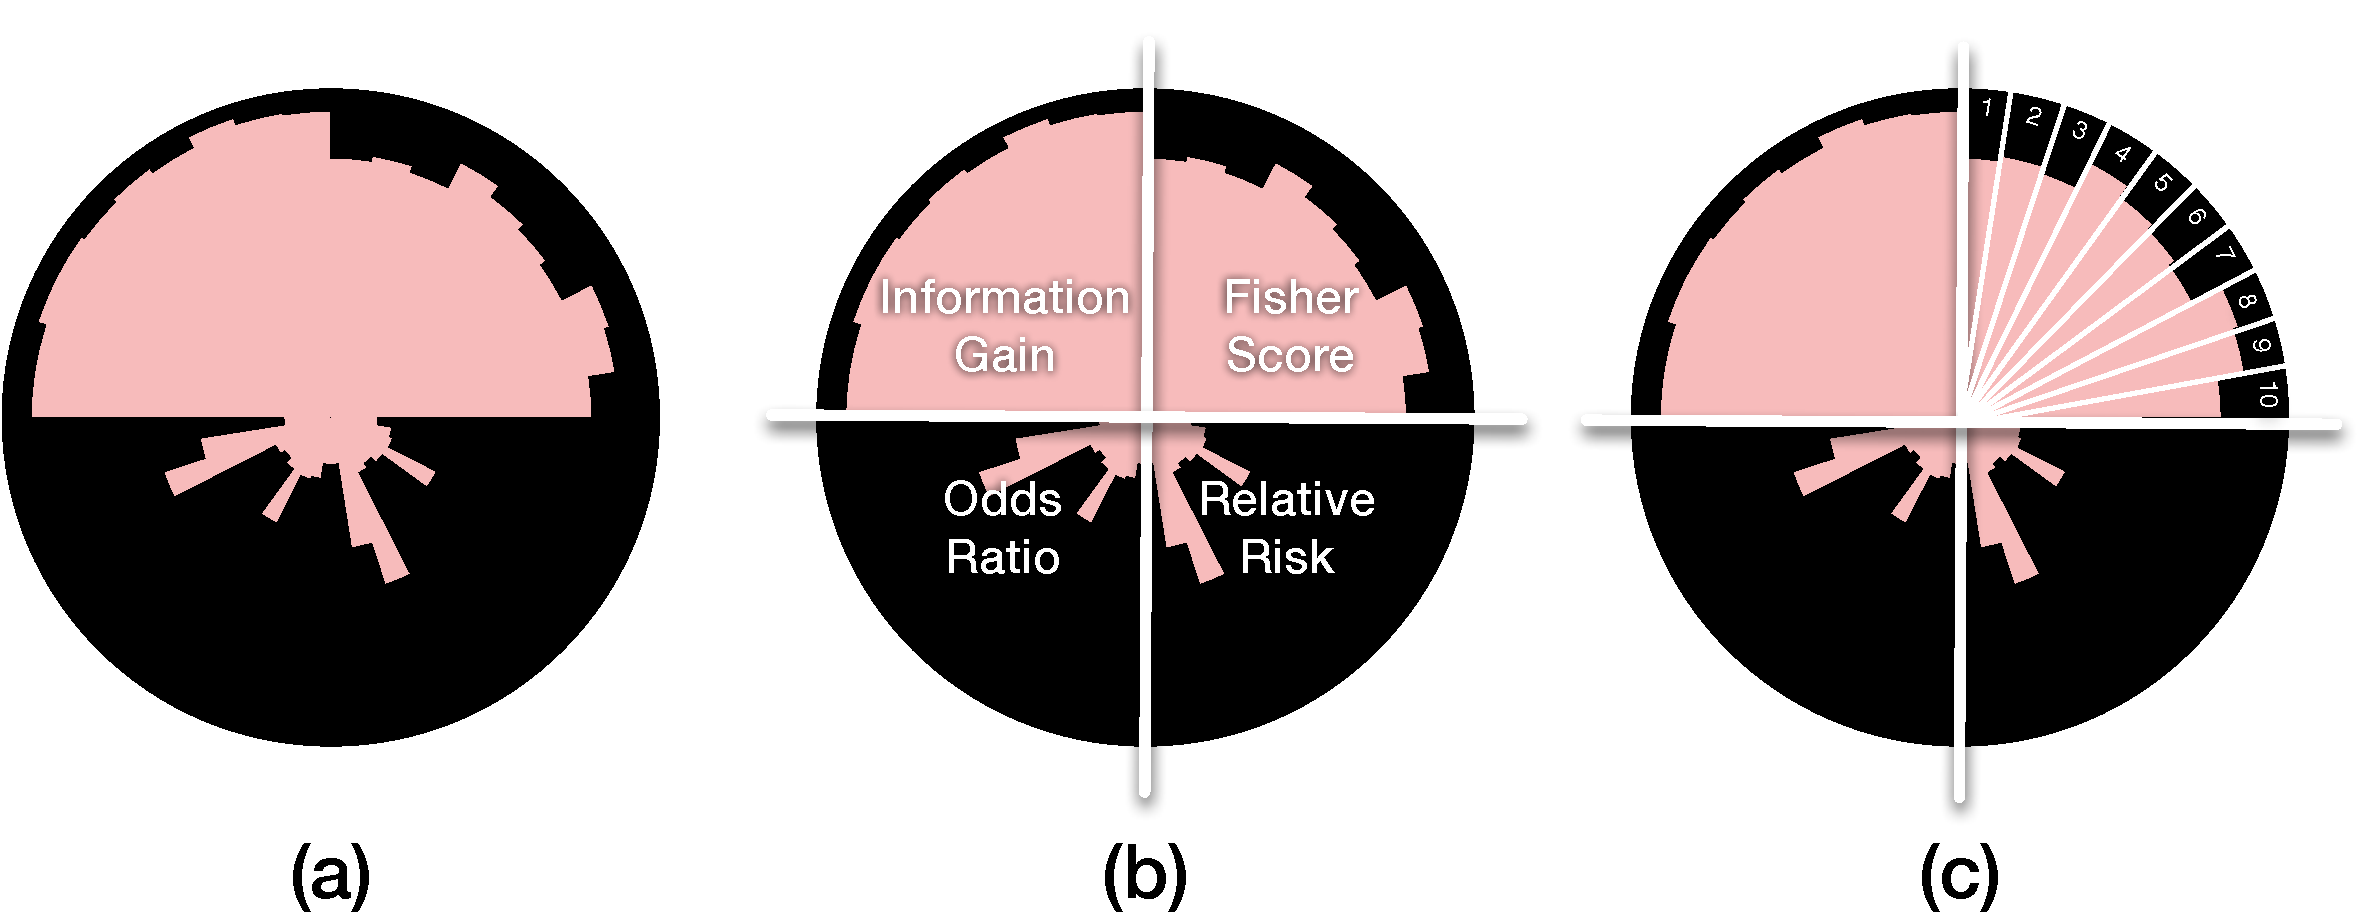
\includegraphics[width=0.95\linewidth]{infuse/glyph-key}
\caption[How to read the glyph representation of \infuse.]{
(a) The glyph representation of a feature in the \infuse system.
(b) Multiple models for each feature are represented as \emph{model sections}.  In this example, the feature is divided into four sections, as it was ranked by four feature selection algorithms (Information Gain, Fisher-Score, Relative Risk, and Odds Ratio.).
(c) Each section is further divided into \emph{fold slices} representing each of the cross-validation folds. Each fold slices features a inward-filling bar that represents the rank of this feature in that fold.
A longer bar implies the feature has a better rank.  If no bar appears, the feature was unranked in the fold, and thus did not meet the importance threshold.
\vspace*{2em}
}
\label{fig:glyph-key}
\end{figure}

\begin{figure}[ht]
\begin{subfigure}{0.23\linewidth}
\centering
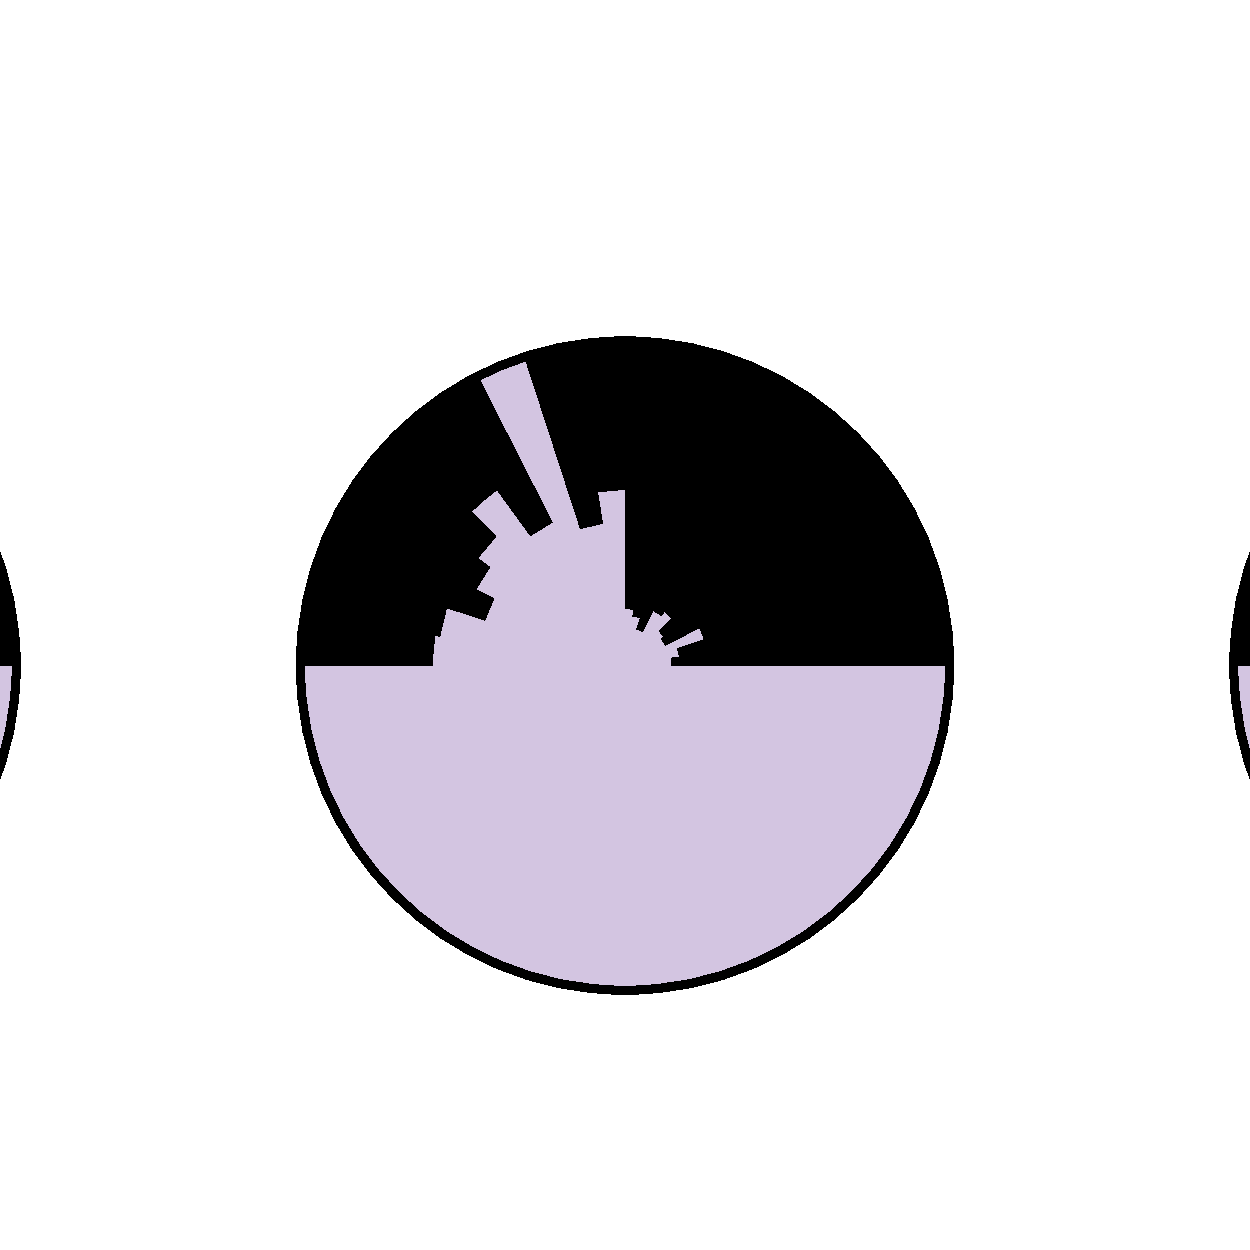
\includegraphics[width=\linewidth,clip,trim={2.4cm 4cm 1.7cm 4cm}]{infuse/g0}
\caption{}
\label{subfig:inward}
\end{subfigure}%
\hspace*{0.01\linewidth}%
\begin{subfigure}{0.23\linewidth}
\centering
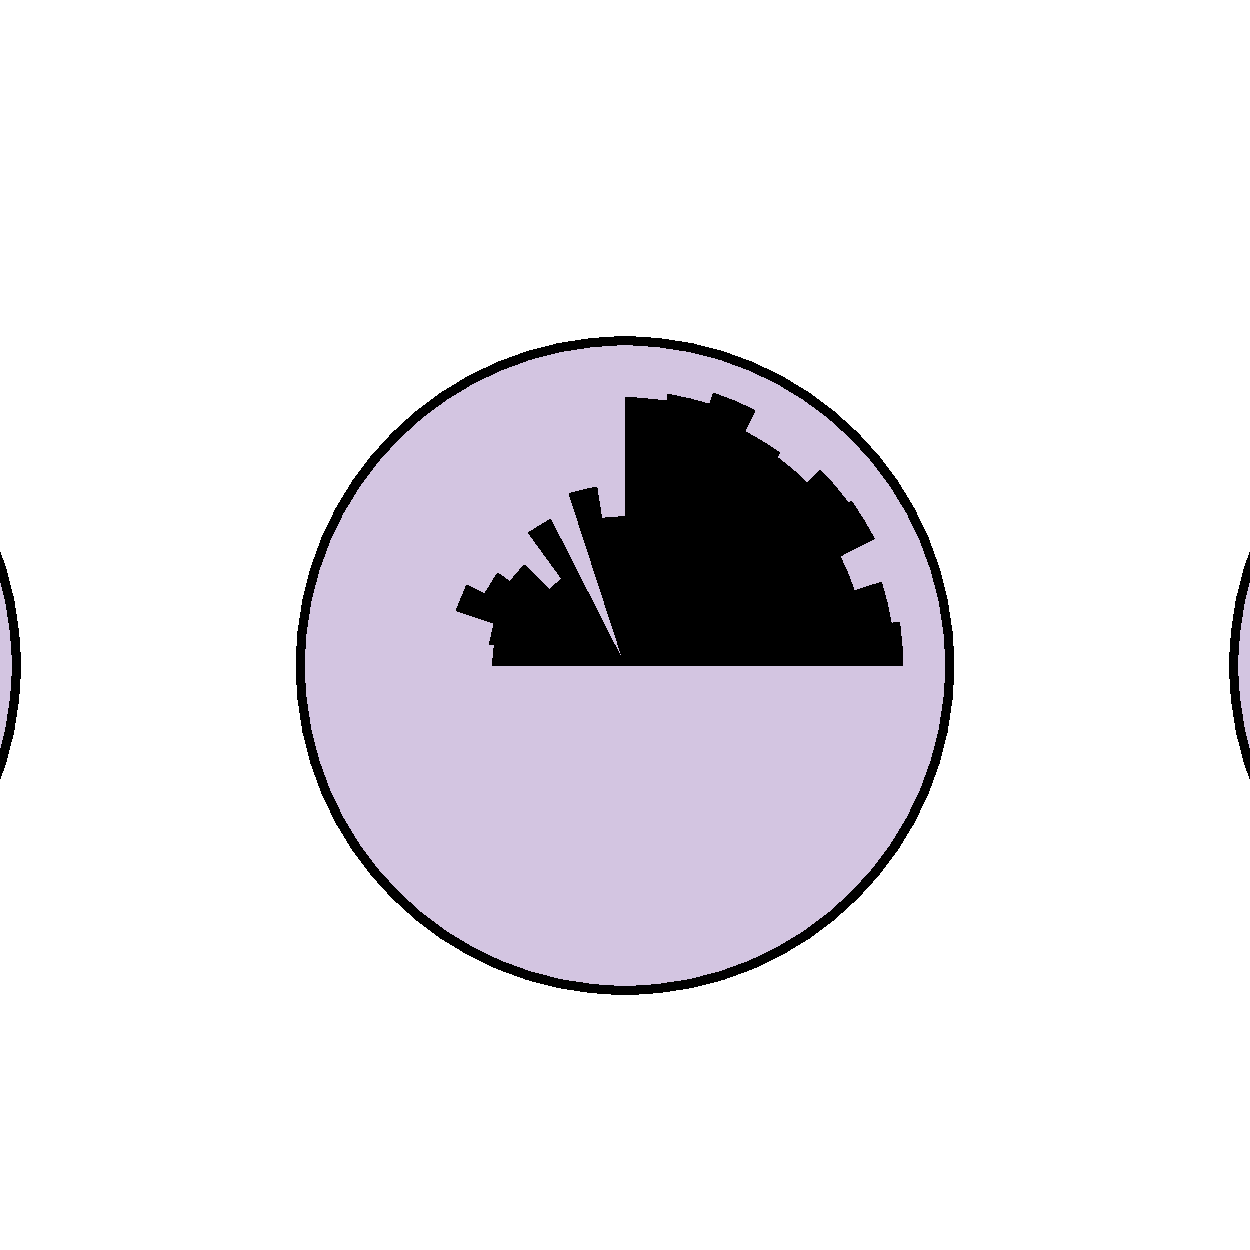
\includegraphics[width=\linewidth,clip,trim={2.4cm 4cm 1.7cm 4cm}]{infuse/g1}
\caption{}
\label{subfig:pie}
\end{subfigure}%
\hspace*{0.01\linewidth}%
\begin{subfigure}{0.23\linewidth}
\centering
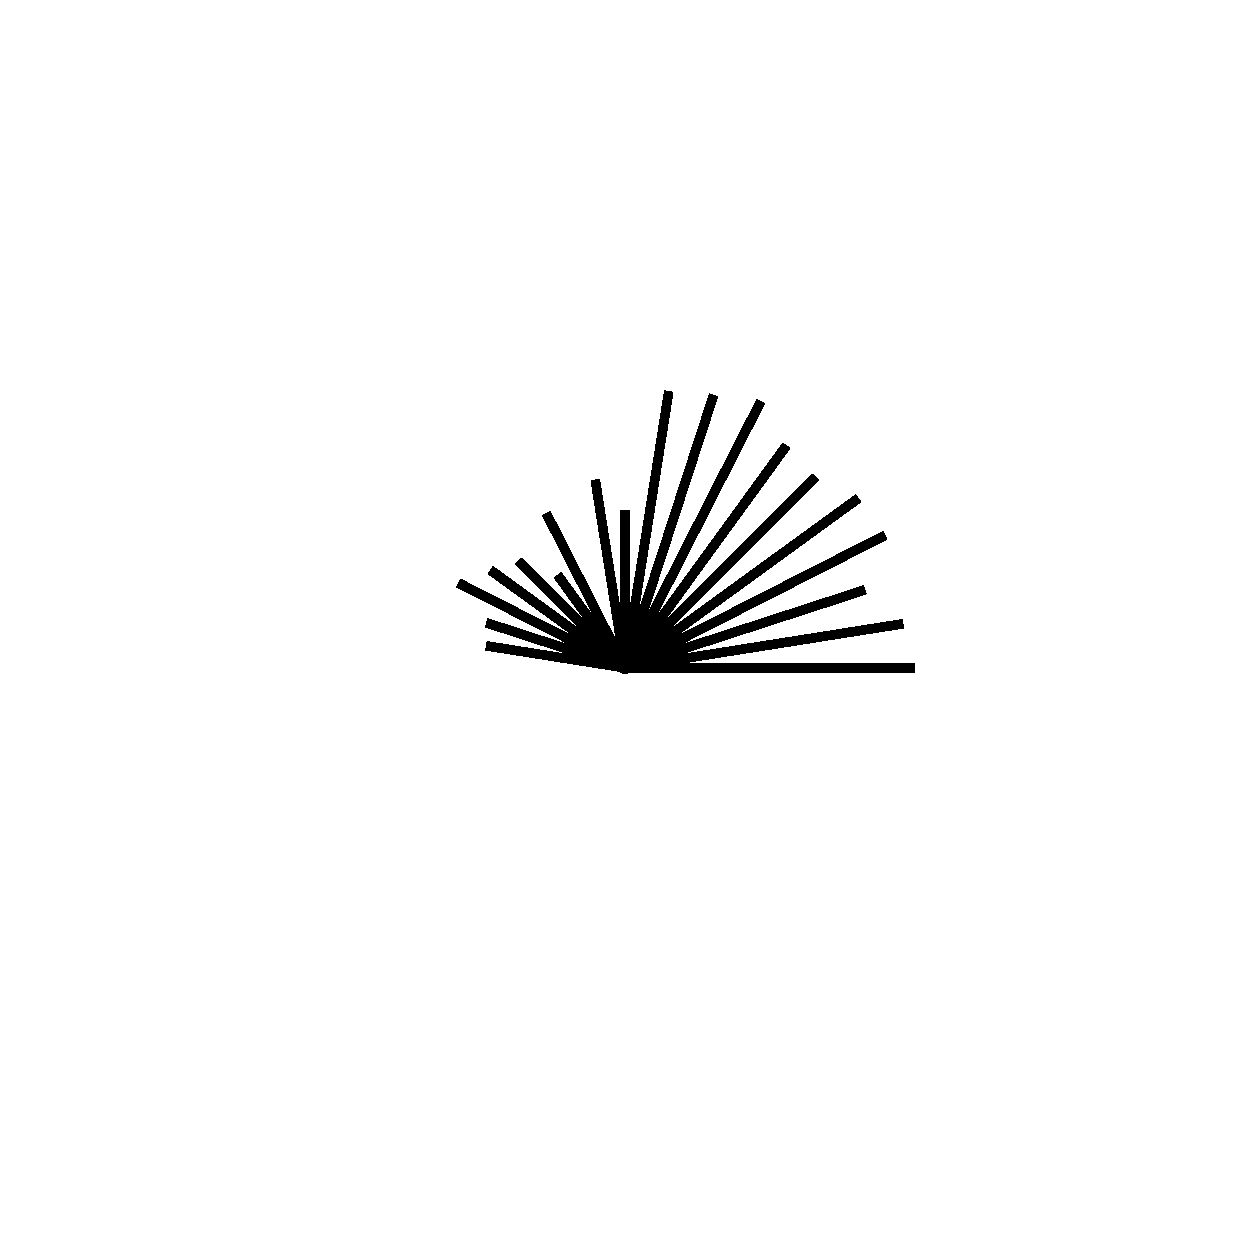
\includegraphics[width=\linewidth,clip,trim={2.4cm 4cm 1.7cm 4cm}]{infuse/g2}
\caption{}
\label{subfig:star}
\end{subfigure}%
\hspace*{0.01\linewidth}%
\begin{subfigure}{0.23\linewidth}
\centering
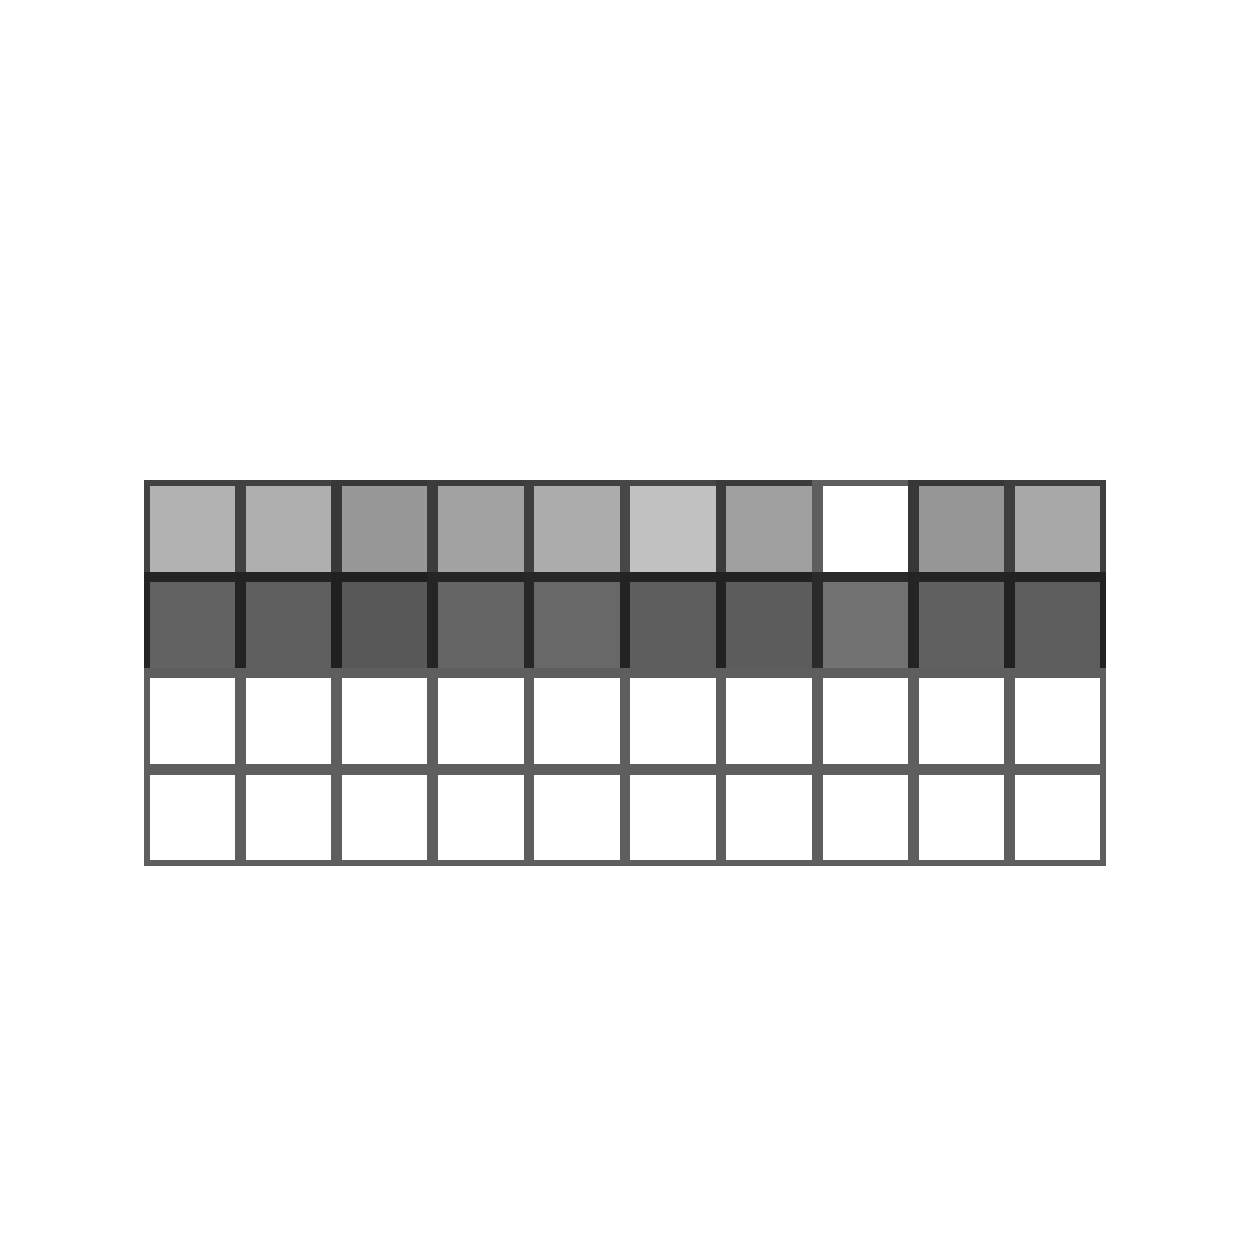
\includegraphics[width=\linewidth,clip,trim={2.4cm 4cm 1.7cm 4cm}]{infuse/g3}
\caption{}
\label{subfig:matrix}
\end{subfigure}%
\caption[Different glyph designs.]{
Different glyph designs.
\subref{subfig:inward} shows \emph{fold slices} with bars growing from perimeter to center
whereas \subref{subfig:pie} grows from center to perimeter.
\subref{subfig:star} shows a typical starburst glyph and
\subref{subfig:matrix} shows a matrix using luminance to show the ranks.
Note that in \subref{subfig:pie} and \subref{subfig:star} it is difficult
to see that this feature is unranked in the third fold from the right in
the top left quadrant.
The values in \subref{subfig:star} are difficult to read because
there is no reference to how big the values are.
Luminance, as used in \subref{subfig:matrix} is a harder perceptual attribute for users
to interpret and distinguish than length and area are, as used by the other glyphs.
}
\label{fig:glyph_design}
\end{figure}

\subsection{Data and Design}

We provide a brief overview of data types utilized by the system. A predictive model, in our setting, is a model trained and validated with machine learning using a high number of features as an input to train the model. These features are the primary data items of \infuse. Each feature has a label representing the feature name (e.g. Diabetes), a category to which the feature belongs to (e.g. Diagnosis), and a subtype (e.g. Problem List, the health problems that led to the diagnosis).

Feature selection algorithms receive as an input the whole set of existing features and return a subset of features selected and ranked according to their estimated predictive power. Since in our setting we use the output of multiple algorithms at once, each feature can further be described by the rankings they receive from all these algorithms (where features that are not selected are marked as unranked). Furthermore, since cross-validation is used, each feature actually gets ranked multiple times by each algorithm, leading to a total number of $\#\textit{feature selection algorithms} \times \#\textit{folds}$ ranks that quantitatively describe each feature.


%As described above in \ref{sec:motivation_healthcare}, feature selection works the features can be ranked by multiple feature selection algorithms, across multiple cross-validation folds. More precisely, for a pre-defined set of feature selection algorithms, each feature can further be described by the which results in number of ranks per feature. If a feature is not selected by a feature selection algorithm, it means it did not reach the threshold to be considered information and is unranked.

The predictive models built using the output generated by feature selection also provide useful information that we use in our system. Each feature set generated by the process described above is used as an input to a classification algorithm. The algorithm builds a model that corresponds to the specific pair of feature set and classification algorithm used for its training. The classifier, in turn, can be described in terms of its performance using the Area Under Curve (AUC), a measure that is commonly used by modelers to give numerical performance scores to models \cite{kuhn2013applied}.

%Each model within a cross-validation fold is then scored by multiple classification algorithms in the form of AUC (the Area Under Curve of the false positive rate in relation to the true positive rate) scores.  The overall quality of a feature set is the average area under curve for all used classification algorithms.

The primary goal of \infuse is to visualize this information so that users can understand the predictive power of features in their models. The user interfaces is organized around three main coordinated views as shown in Figure~\ref{fig:system}: the \textit{Feature View} provides a way to visualize an overview of all features providing information about their attributes and ranking received from feature selection; the \textit{List View} provides a sorted list of all features to get easy access to their labels and to assist the user in searching features according to some predefined criteria like their name or category; the \textit{Classifier View} provides access to the quality scores of each model built using the process described above. The views are coordinated so that selections in one view are propagated to all the other views. In the following we provide additional information about the design of each view.

% Seeing how features perform in various models
% is important for our system.
% Therefore, features showing their ranks in different models are
% first-class citizens of the visualization and for every feature
% the ranks can be seen at any time.
% Features can also be selected by the user to see or build feature sets.
% Selections are linked and visible throughout the tool.

% The system is split into three main components.
% The central part is the feature view that shows all features
% with their ranks as glyphs.
% The positions of the features can be sorted by type and
% overall importance to get an overview or they can
% be positioned on a scatterplot to show additional data about them.
% The type and subtype can be inferred from the glyph.
% Further information about a feature, like name,
% statistics about the rankings which are used as axes for the scatterplot,
% and exact rank numbers can be displayed as tooltip.

% Features are also shown in the list view on the right side.
% This view focuses more on the names of the features but
% shows also the glyph as orientation.
% The order of the elements in the list can be chosen to be by type,
% subtype, and then name, or by showing currently selected features on
% top, ranked by their importance.

% Seeing the area under curve for different
% feature sets is also an important task, since the quality
% of those sets is measured by it.
% In the bottom right corner the area under curve of all models
% is shown for every classification algorithm as matrix.
% Models can be picked to select the features of the corresponding set.

\begin{figure*}[ht]
\centering
\begin{subfigure}{0.24\linewidth}
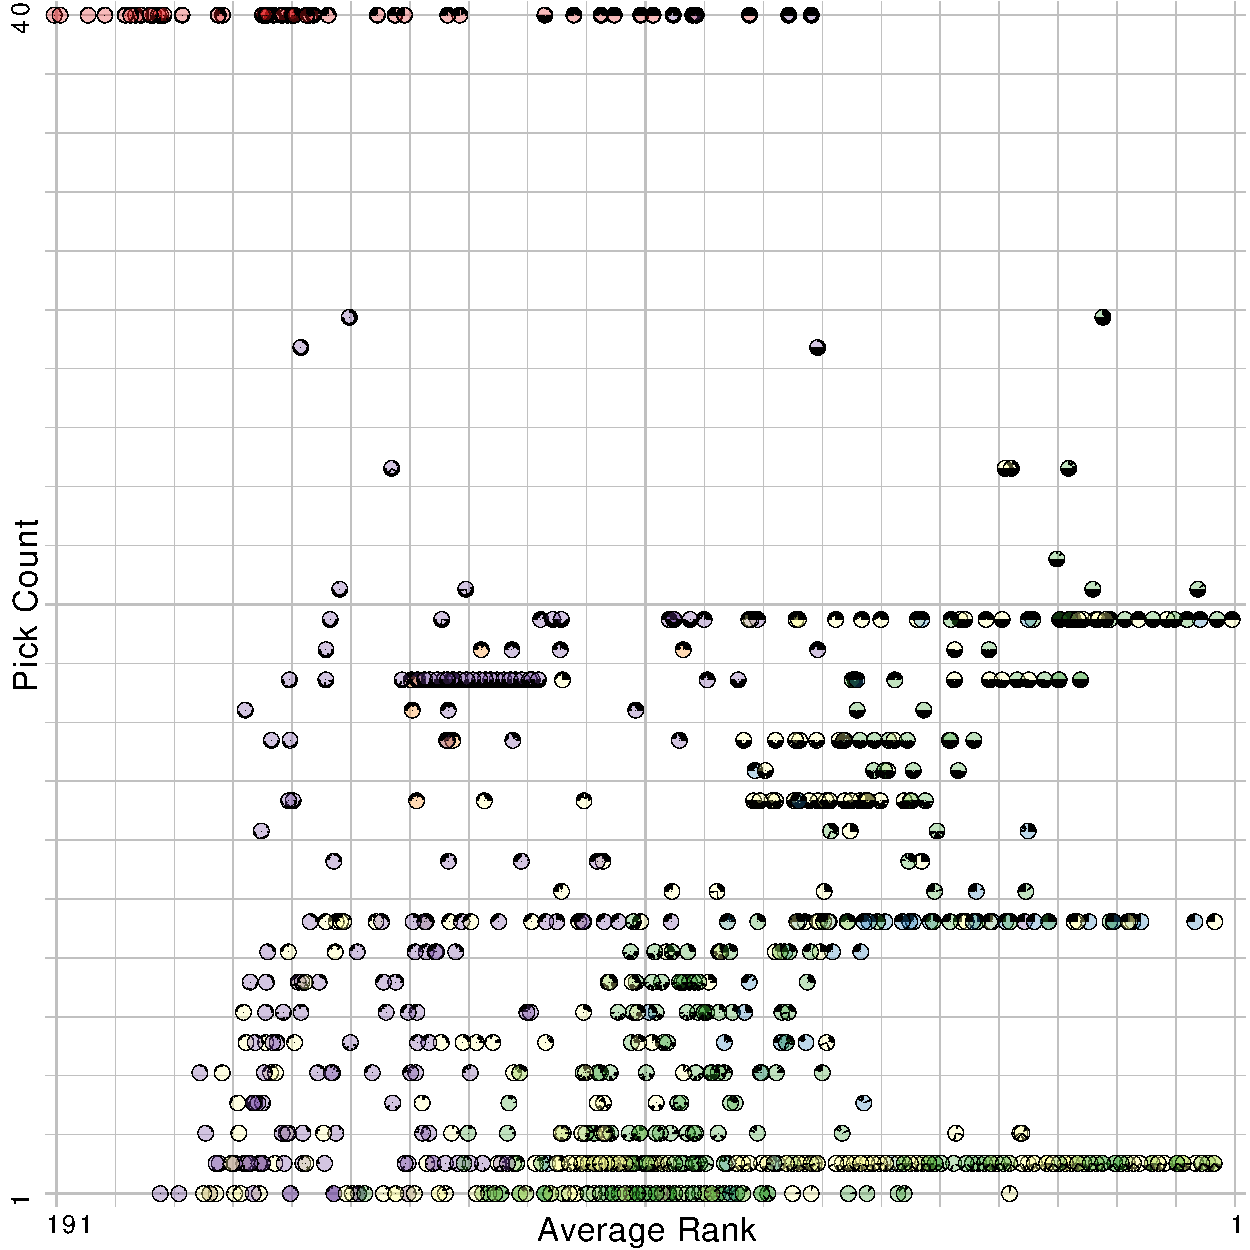
\includegraphics[width=\linewidth]{infuse/ap}
\label{subfig:ap}
\end{subfigure}%
~%
\begin{subfigure}{0.24\linewidth}
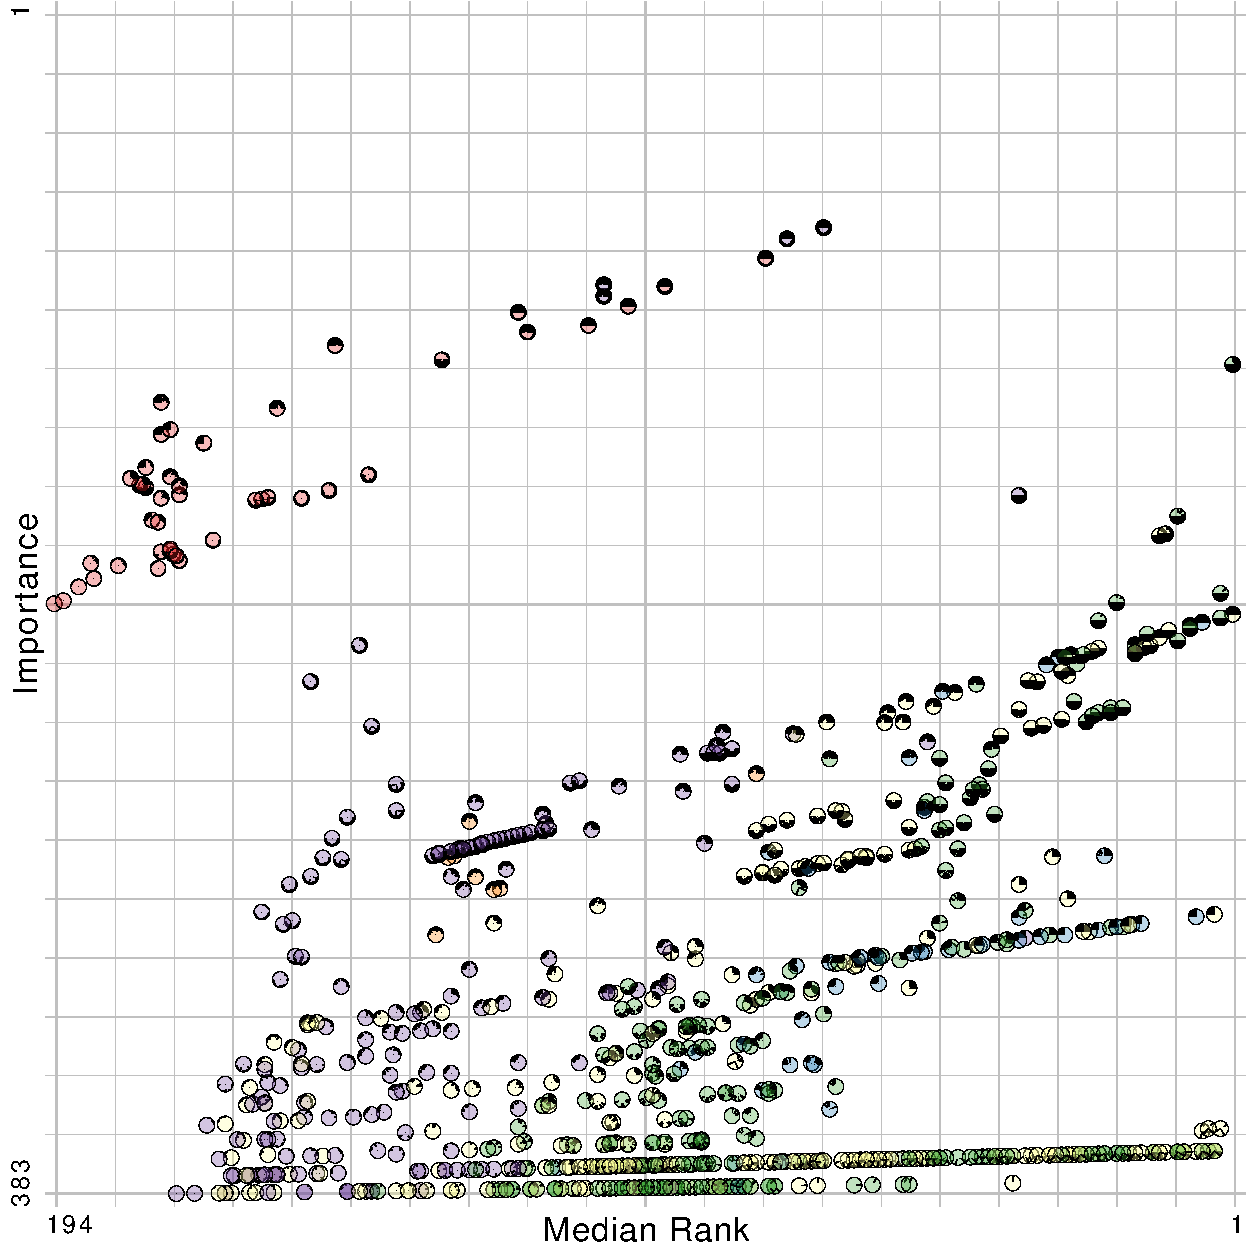
\includegraphics[width=\linewidth]{infuse/mi}
\label{subfig:mi}
\end{subfigure}%
~%
\begin{subfigure}{0.24\linewidth}
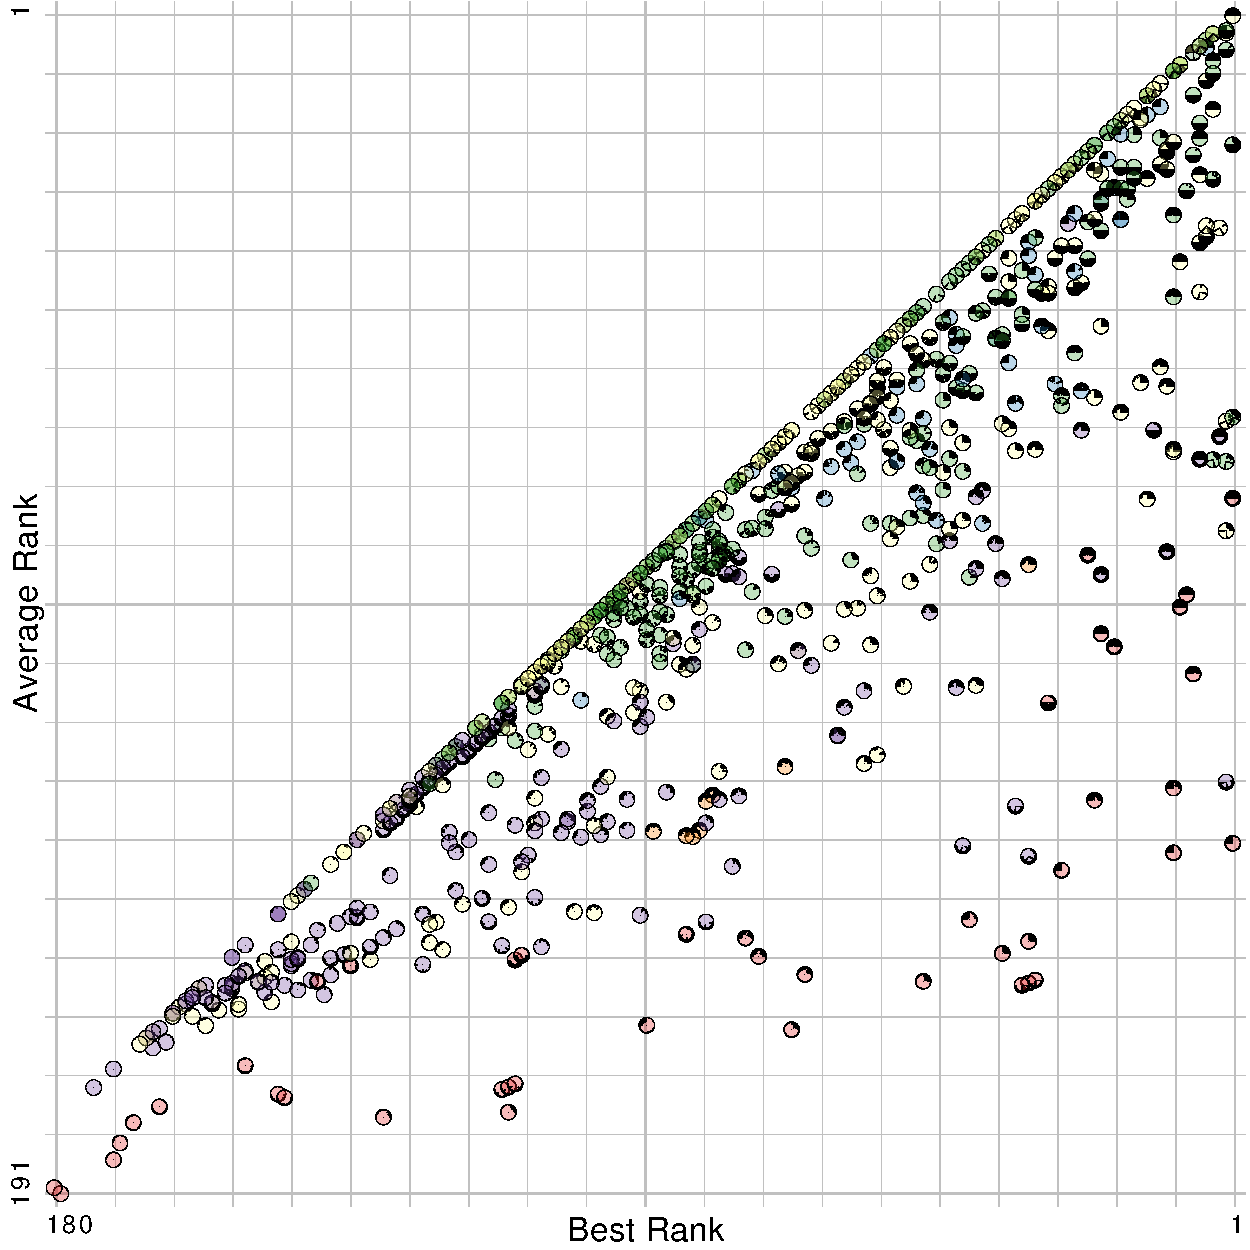
\includegraphics[width=\linewidth]{infuse/ba}
\label{subfig:ba}
\end{subfigure}%
~%
\begin{subfigure}{0.24\linewidth}
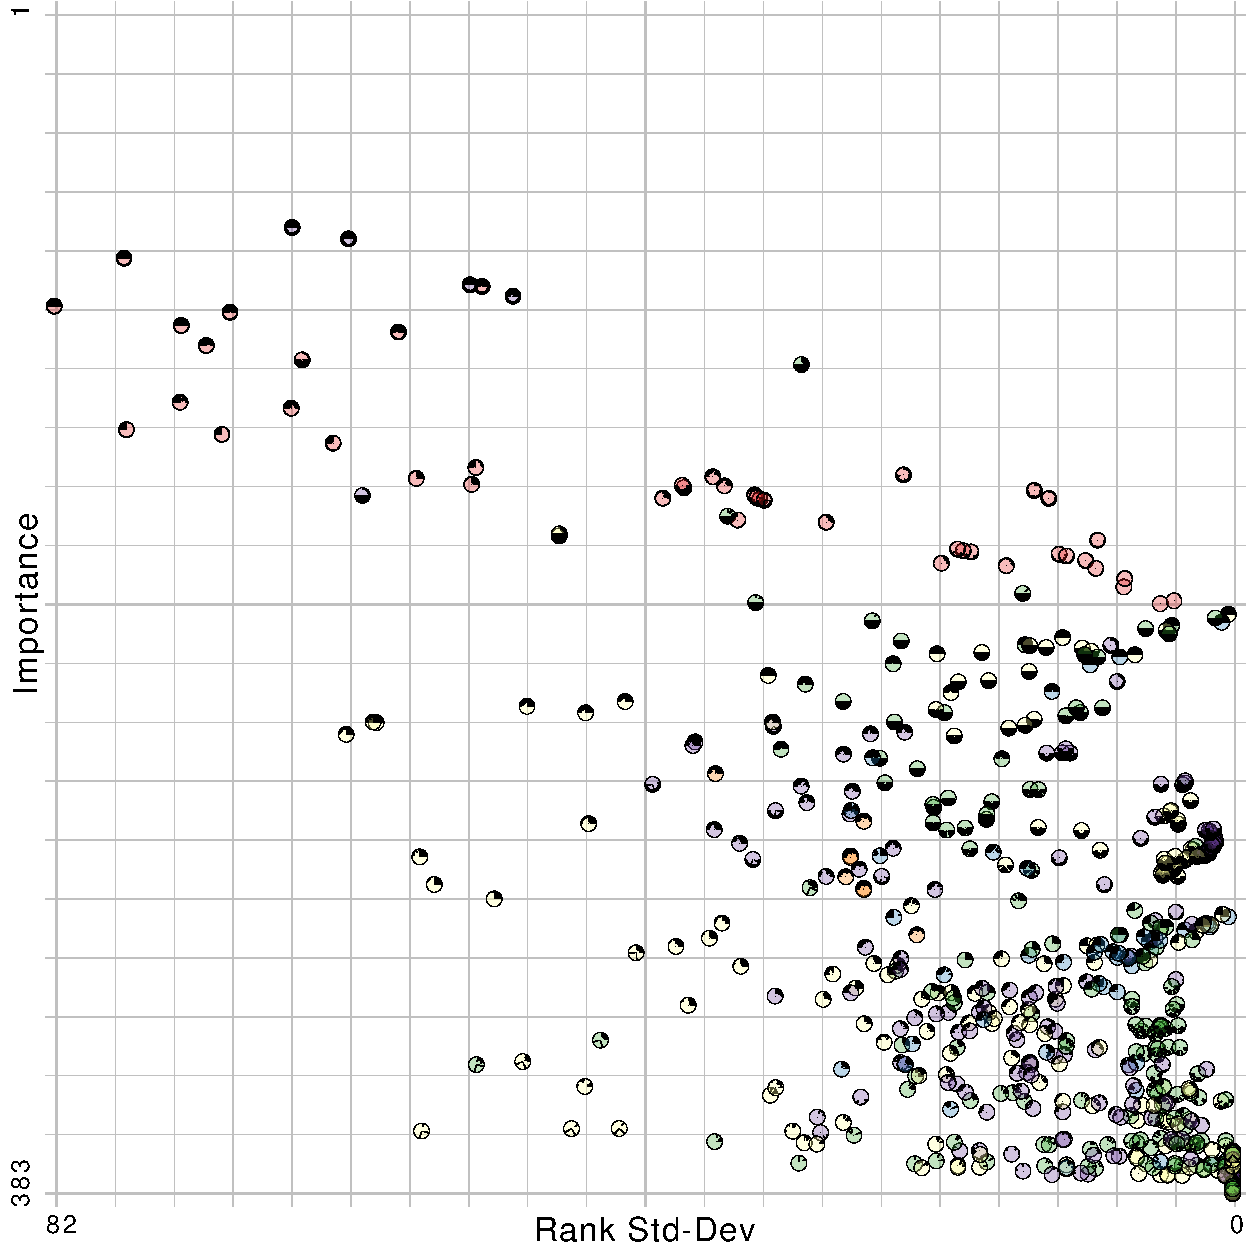
\includegraphics[width=\linewidth]{infuse/si}
\label{subfig:si}
\end{subfigure}
\caption{
Different axis combinations for the scatter-plot layout.
In \subref{subfig:ap} the average rank is plotted against the pick count.
Most of the features appear in the lower half because features are rarely picked by more than two algorithms in this example.  The bottom-right shows features that are only chosen
by two models but were ranked very high by them.
\subref{subfig:mi} shows the median rank plotted against the importance.
Notice that the plot looks similar to \subref{subfig:ap} since importance
is a combination of the axes from \subref{subfig:ap}.
The axes in \subref{subfig:ba} are best rank versus average rank.
Features can only appear below the diagonal.
The standard deviation of the ranks is plotted against the importance
in \subref{subfig:si}.
The peak to the bottom right corner consists of features that are rarely
picked and therefore have lower variance.
The peak to the top right consists of features that
are consistently high ranked.
}
\label{fig:scatter}
\end{figure*}

\subsection{Feature View}
The primary component of \infuse is the \textit{Feature View}, a zoomable visualization that displays all features as glyphs. Each glyph represents a feature from the original data set and is designed to provide the information outlined above. The main purpose of the feature view is to allow comparison between features and detection of interesting commonalities and differences in terms of how the algorithms rank them. The view allows the user to display the feature set according to two different configurable layouts: a grid layout (the default), which favors legibility, and a scatter plot layout which aims at laying out and grouping the features according to various statistics we collect from the ranks. In the following sections, we describe the design of the glyph as well as the different layouts.

% The design of the glyphs is discussed in Section~\ref{sec:glyphdesign}.
% The glyphs can be laid out in two different ways in the visualization,
% ordered by type and overall importance as described in
% Section~\ref{sec:rankedlayout}, or by positioning them
% on a scatterplot with user defined axes
% (Section~\ref{sec:scatterplotlayout}).
% By clicking on features, the user can toggle its selection.
% A group of features can be selected at once via lasso selection.

\subsubsection{Feature Glyph Design}\label{sec:glyphdesign}
% \adam{on our next phonecall, lets discuss why you call these starburst charts.  there is nothing hierarchical about this data.}
% \adam{note:  low and high ranks are used in misleading ways.  i'm putting this note to make sure we double-check to make sure we're consistent.}
As described in Section \ref{sec:motivation_healthcare}, the features are ranked by multiple feature selection algorithms and across multiple cross-validation folds.  \infuse's glyph design embeds all of this information in a circular glyph that shows all the rankings obtained from each algorithm/fold pair. As shown in Figure~\ref{fig:glyph-key}(a), the glyph is divided into equally-sized circular segments; where each segment represents one of the ranking algorithms.
For instance, in Figure \ref{fig:glyph-key}(b), since the feature was ranked by four feature selection algorithms, the circular glyph is divided into four sections. Each of these sections are then divided further into a \emph{fold slice} for each cross-validation fold. For instance, in Figure \ref{fig:glyph-key}(c), each feature selection algorithm was executed on 10 cross-validation folds, therefore there are 10 fold slices.

Within each fold slice, there is an inward-growing bar (that is, starting from the perimeter and growing towards the center) that represents the rank of the feature in a particular fold. For example, in Figure \ref{fig:glyph-key}(c), the feature is higher ranked in Fold 3 than in Fold 4 as the bar in Fold 3 stretches closer towards the center than in Fold 4. Features that are unranked, because their scores are too low to meet the minimum threshold requirement of the algorithm, are represented as empty slices with no bars. We designed fold slices with inward-growing bars on purpose to help distinguishing between slices with empty values from those with low values. During our design iterations we realized in fact that outward pointing bars would make this distinction too hard to make. Since the information of whether a features is picked up by an algorithm is crucial for its interpretation we decided to opt for this design.

%this way on purpose to have bars growing from the perimeter to the center of the circle so that folds with poor ranks can be easy detected since a fold slice has greater area closer to the perimeter.  This makes it possible to identify the basic properties of a feature selection model even when the interface is zoomed-out.



% Features are shown as inward growing starburst pie chart glyphs showing their ranking in the different models. Each pie slice represents one model. The better the rank of the feature the more the slice expands towards the center of the glyph \emph{ie.} when the feature is ranked as number one by the model the corresponding slice has the same radius as the glyph.
% If the feature is not ranked by the model the slice is not shown.
% Letting slices grow from the outside to the inside makes
% low ranks easier to read since a pie slice has a greater area at the outside.
% This enables to see low ranks and identify their model even when
% the visualization is zoomed out.
% For pie slices growing towards the outside it is difficult to
% identify the model when a rank is low.
% Consider a feature that is ranked very low in only one
% model and unranked in the other models.
% When zoomed out only a dot in the center of the glyph is visible.
% This dot could grow in any direction representing any model.
% Also, as shown in Figure~\ref{fig:glyph_design},

% Figure \ref{subfig:pie} shows an example of a glyph where the fold slices grow from the center towards the perimeter. From the figure one can see that distinguishing empty values is harder with this solution than the one we selected.

%Consider the situation where there is a lowly-ranked feature only ranked in one fold slice section.  When zoomed-out, the glyph would just appear as a circle with a dot in the center, and the user would not know which model or fold ranked the feature.

%Furthermore, it is difficult to see in which fold a feature is unranked when the surrounding models rank the feature.

Multiple glyph designs were considered and tested within \infuse.  For instance, Figure \ref{subfig:pie} shows an example of a glyph where the fold slices grow from the center towards the perimeter.
This makes it difficult to identify fold slices with poor ranks.
Consider the situation where there is a lowly-ranked feature only ranked in one fold slice section.  When zoomed-out, the glyph would just appear as a circle with a dot in the center, and the user would not know which model or fold ranked the feature.  Furthermore, it is difficult to see in which fold a feature is unranked when the surrounding models rank the feature.  Other glyph designs that were tried involve a star glyph (Figure \ref{subfig:star}) and a matrix glyph (Figure \ref{subfig:matrix}).  The star glyph was less effective as users were not afforded a reference point for the maximum ranking and the design leads to some visual artifacts (like high density in the center and lower density in the outer part).
The matrix glyph was less effective, as perceiving differences is more difficult when using luminance than length and area as we do in our final design.

%Furthermore, both of these charts were also less suited for a zoomable user interface than the chosen design.

Users can gain more details about each section and slice by hovering over the region of interest to view an informative tooltip. Furthermore, an overview key is available to remind users of the position of each model type. The background color of the glyph corresponds to the subtype of the feature and a color key can also be shown as a reference to remember the meaning of the color coding (see bottom-left corner of Figure~\ref{fig:system}).

% Pie slices are ordered by feature selection
% algorithm first and then by fold.
% This groups all results from one feature selection algorithm together
% and creates quadrants which can be used for reasoning.
% A key for those quadrants can be shown in the visualization
% and when hovering a slice with the mouse the identity of the model
% and the rank is shown in the tooltip.

% A circle with the radius of the glyph is drawn to distinguish glyphs
% from each other and defines the value bounds.


% Using colors to show ranks, for example as cell colors of a
% feature selection algorithm by fold matrix,
% is not as easy to read as the presented glyph.
% Also, normal starburst glyphs do not work very well when the
% visualization is zoomed out as the lines become thinner and harder to see.

\vspace*{1em}
\subsubsection{Ranked Layout}\label{sec:rankedlayout}
The first layout available to users is the ranked layout, which arranges glyphs by their feature type, and sorts them by their overall importance.  The name of the feature type is shown at the first position in the group, after that the features are laid out row-first in a grid-like manner, as shown in Figure \ref{fig:system}. This space-filling approach results in features that are always visible without overlaps.

Features within a group are sorted by their importance. Importance is computed as average rank with
penalized unranked features:
\[
rank_{best} = \min_{m \in M \times V, f \in F}{[rank_{m}(f)]}
\]\[
i(f) = \dfrac{1}{| M \times V |}[
2 \cdot rank_{best} \cdot
unranked_{M \times V} (f)
+ \sum_{m \in M \times V} rank_{m}(f)
]
\]
where $M$ is the set of models, $V$ is the set of cross-validation folds,
$F$ is the set of features,
$rank_{m}(f)$ is the rank of a feature $f$ in the combined model
and cross-validation fold $m$,
and $unranked_{M \times V} (f)$ is the number
of such combined models that did not choose $f$.
Assume $rank_{m}(f) = 0$ for unranked features $f$
in the combined model $m$ only when computing $i(f)$.
Note that a small value for $i(f)$ means higher importance.
The optimal value is $1$.

\subsubsection{Scatterplot Layout}\label{sec:scatterplotlayout}
The second layout available to users is the scatterplot layout, where users can select choices for both axes of the scatterplot.  The choices for axes include:

\begin{itemize}
\item the \emph{average rank} of a feature\\
(ignores unranked folds and models)
\item the \emph{pick count} of the number of combined
models\\and cross-validation folds that picked the feature
\item the \emph{importance} of a feature (defined above)
\item the \emph{best rank} of the feature
\item the \emph{median rank} of the feature\\
(ignores unranked folds and models)
\item the \emph{standard deviation} of the feature's ranks\\
(ignores unranked folds and models)
\end{itemize}

By default, the average rank is chosen for the horizontal axis and
the pick count is chosen for the vertical axis, as shown in Figure \ref{fig:usecase2}.  This combination of axes led to the most insights during the case studies.  However, if users choose to select different axes or pivot to a different layout, animation is used for the transition.  By using slow-in and slow-out animation, users are given time to anticipate the movement direction of the feature, and are able to track features during the transition easily.

% The combination of those axis contents give the most insights.
% The values of the axes are mapped from the
% minimum to the maximum value.
% The lower left corner of the scatter-plot is consistently the
% worst values of both axis and the top left corner is always the best
% values of both axis contents.

\subsubsection{Interaction}
The Feature View provides a number of interactions.
Zooming and panning enables a user to get an overview of the
displayed data and focus on the details of a small number of glyphs.  This exploration can be reset by clicking on the
``Reset View" button, or double clicking on the background. Double clicking on a feature glyph zooms in on the feature so that it fills the viewport.
In addition, a tooltip is shown when a user hovers the mouse
over a glyph. This tooltip provides information about the name, type,
and subtype of the represented feature, as well as all of the statistical
information used for the scatterplot layout. Hovering over a fold slice
in the glyph gives further information about the feature selection algorithm,
the cross-validation fold, and the feature's rank in question.  In order to select features for interactive model building
(see Section~\ref{sec:imb}) the user can click on glyphs to toggle
the selection or use a lasso gesture to select a group of features.
As mentioned in the previous section, users can change the
layout of the glyphs with the buttons below the Feature View.

\subsection{List View}
A simple yet important view of features is the List View, which provides a sorted list of all features, useful for selecting features by name.  Each list item contains the name of the features along with its glyph.  The selection of a feature can be toggled in the list by clicking its list item.  As the selection of features is linked between views, this sorted and labeled view supports users finding particular features of interest and highlighting them in the complementary views.

The list view can be sorted in a few different ways. By default, features are first sorted by
the type of the feature, then by its subtype, and finally by its name.  Users can also sort the list by selection, which means currently selected features are displayed at the top and the unselected features appear after them.  Within these groups, the features are then sorted by their importance.

In addition to sorting, a user can filter the list view via the search box on
the top.
Search terms are separated by white-spaces and the list view
shows all features that contain all search terms in the name, type, or
sub-type.
The results are ranked by the sum of the inverse positions
of the search terms within the feature description.
This favors terms occurring at the beginning of the feature's name
and terms that occur multiple times in one feature description
(see the top right panel of Figure~\ref{fig:system} for an example query).

\begin{figure}[t]
\centering
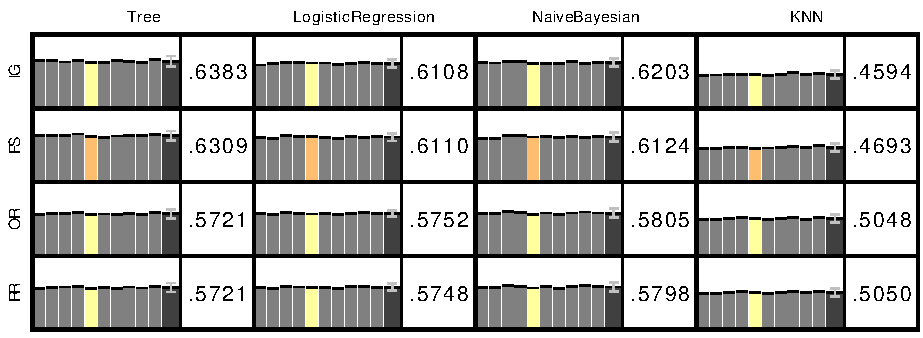
\includegraphics[width=0.8\linewidth]{infuse/classifier}
\caption{The Classifier View displays the results of the classification algorithms for all models.
Rows represent feature selection algorithms and columns represent classification algorithms.
A more detailed description of the cells can be
seen in Figure~\ref{fig:classifier-cell}.
The currently selected model is highlighted in orange, and the results for the same fold in different
feature selection algorithms are highlighted in yellow.  When users select a model, the features that make up the model are highlighted in the Feature and List views.
}
\label{fig:classifier}
\end{figure}

\begin{figure}[b]
\centering
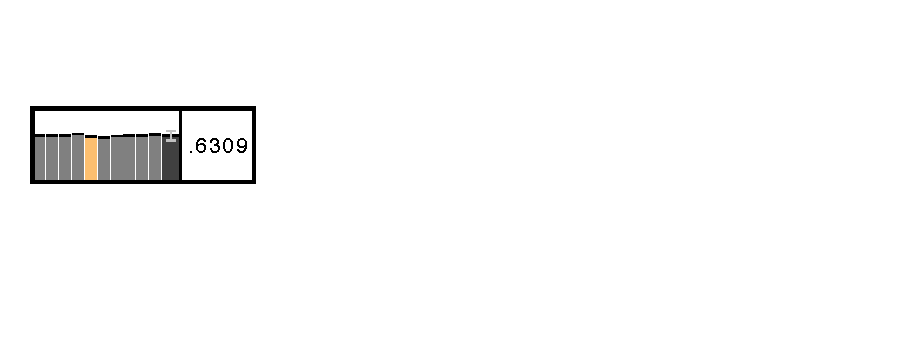
\includegraphics[width=0.5\linewidth]{infuse/classifier-cell}
\caption{
Each cell in the Classifier View represents the scores of a particular model by a particular classifier.
On the left, there is a bar for each of the validation folds.  The height of each bar corresponds to the AUC score for each fold.  Immediately to the right of the fold bars, the thicker and darker bar and its height represents the average value across all folds.  This bar also features an error bar depicting the standard deviation across the folds.  Finally, to the right of the bars, there is a numerical representation of the average AUC score.}
\label{fig:classifier-cell}
\end{figure}

\subsection{Classifier View}

The Feature View and the List View both focus on supporting users to interpret the rankings of features across multiple predictive models.  However, it is also important for users to understand the quality of each model in predicting the appropriate outcome.  The Classifier View, shown in the bottom-right panel of \infuse, is where the quality of each the predictive models can be analyzed.

Typically, predictive models are evaluated using classification algorithms which provide an AUC score (area under ROC curve,
the sensitivity as function of the false positive rate).  Perfect models will have an AUC score of 1, whereas random guessing will have an AUC score of 0.5.  The Classifier View was designed to show AUC scores for each model and fold.

As illustrated in Figure \ref{fig:classifier}, each row of the Classifier View represents the predictive model that resulted from each feature selection algorithm.  Each column represents a classification algorithm.  Multiple classifiers are used because there are a variety of techniques to evaluate models, and in order to avoid biases, \infuse provides the ability to compare the output from multiple classifiers.

Each cell, as shown in Figure \ref{fig:classifier-cell}, has several components.  On the left, there is a bar for each of the validation folds.  The height of each bar corresponds to the AUC score for each fold.  There is also a slightly thicker and darker bar immediately to the right of the fold bars, and its height represents the average value across all folds.  This bar also features an error bar depicting the standard deviation across the folds.  Finally, to the right of the bars, there is a numerical representation of the average AUC score.  As this information is important for predictive modelers to reason about the quality of models, these values are given visual prominence. The bars, however, can be used to also reason about the quality across all folds.

% A matrix showing feature selection algorithms as rows and
% classification algorithms as columns shows those values.
% Each cell is divided into two parts.
% The first part splits the averaged result for one feature selection
% algorithm into the results of the underlying folds.
% The areas under curve for all folds are shown as bar charts.
% The average area under curve for this
% pair of feature selection and classification algorithm is shown
% as slightly thicker and darker bar on the right end of the bar chart.
% An error bar depicts the five times amplified standard deviation
% over the folds.
% The second part shows the average area under curve as actual number.
% This is important for users to be able to directly reason about the values.

Rows are sorted by the average AUC scores across all classification algorithms, so more accurate predictive models appear at the top of this view.  Users can interact with this view in several ways.  Clicking on a fold bar selects all features that were a part of this model and highlights them in the List and Feature views.  The selected fold bar is highlighted in orange, and other scores this fold received by the other classifiers are highlighted in yellow so that they can easily be compared (as shown in Figure~\ref{fig:classifier}.)

\begin{figure}[ht]
\centering
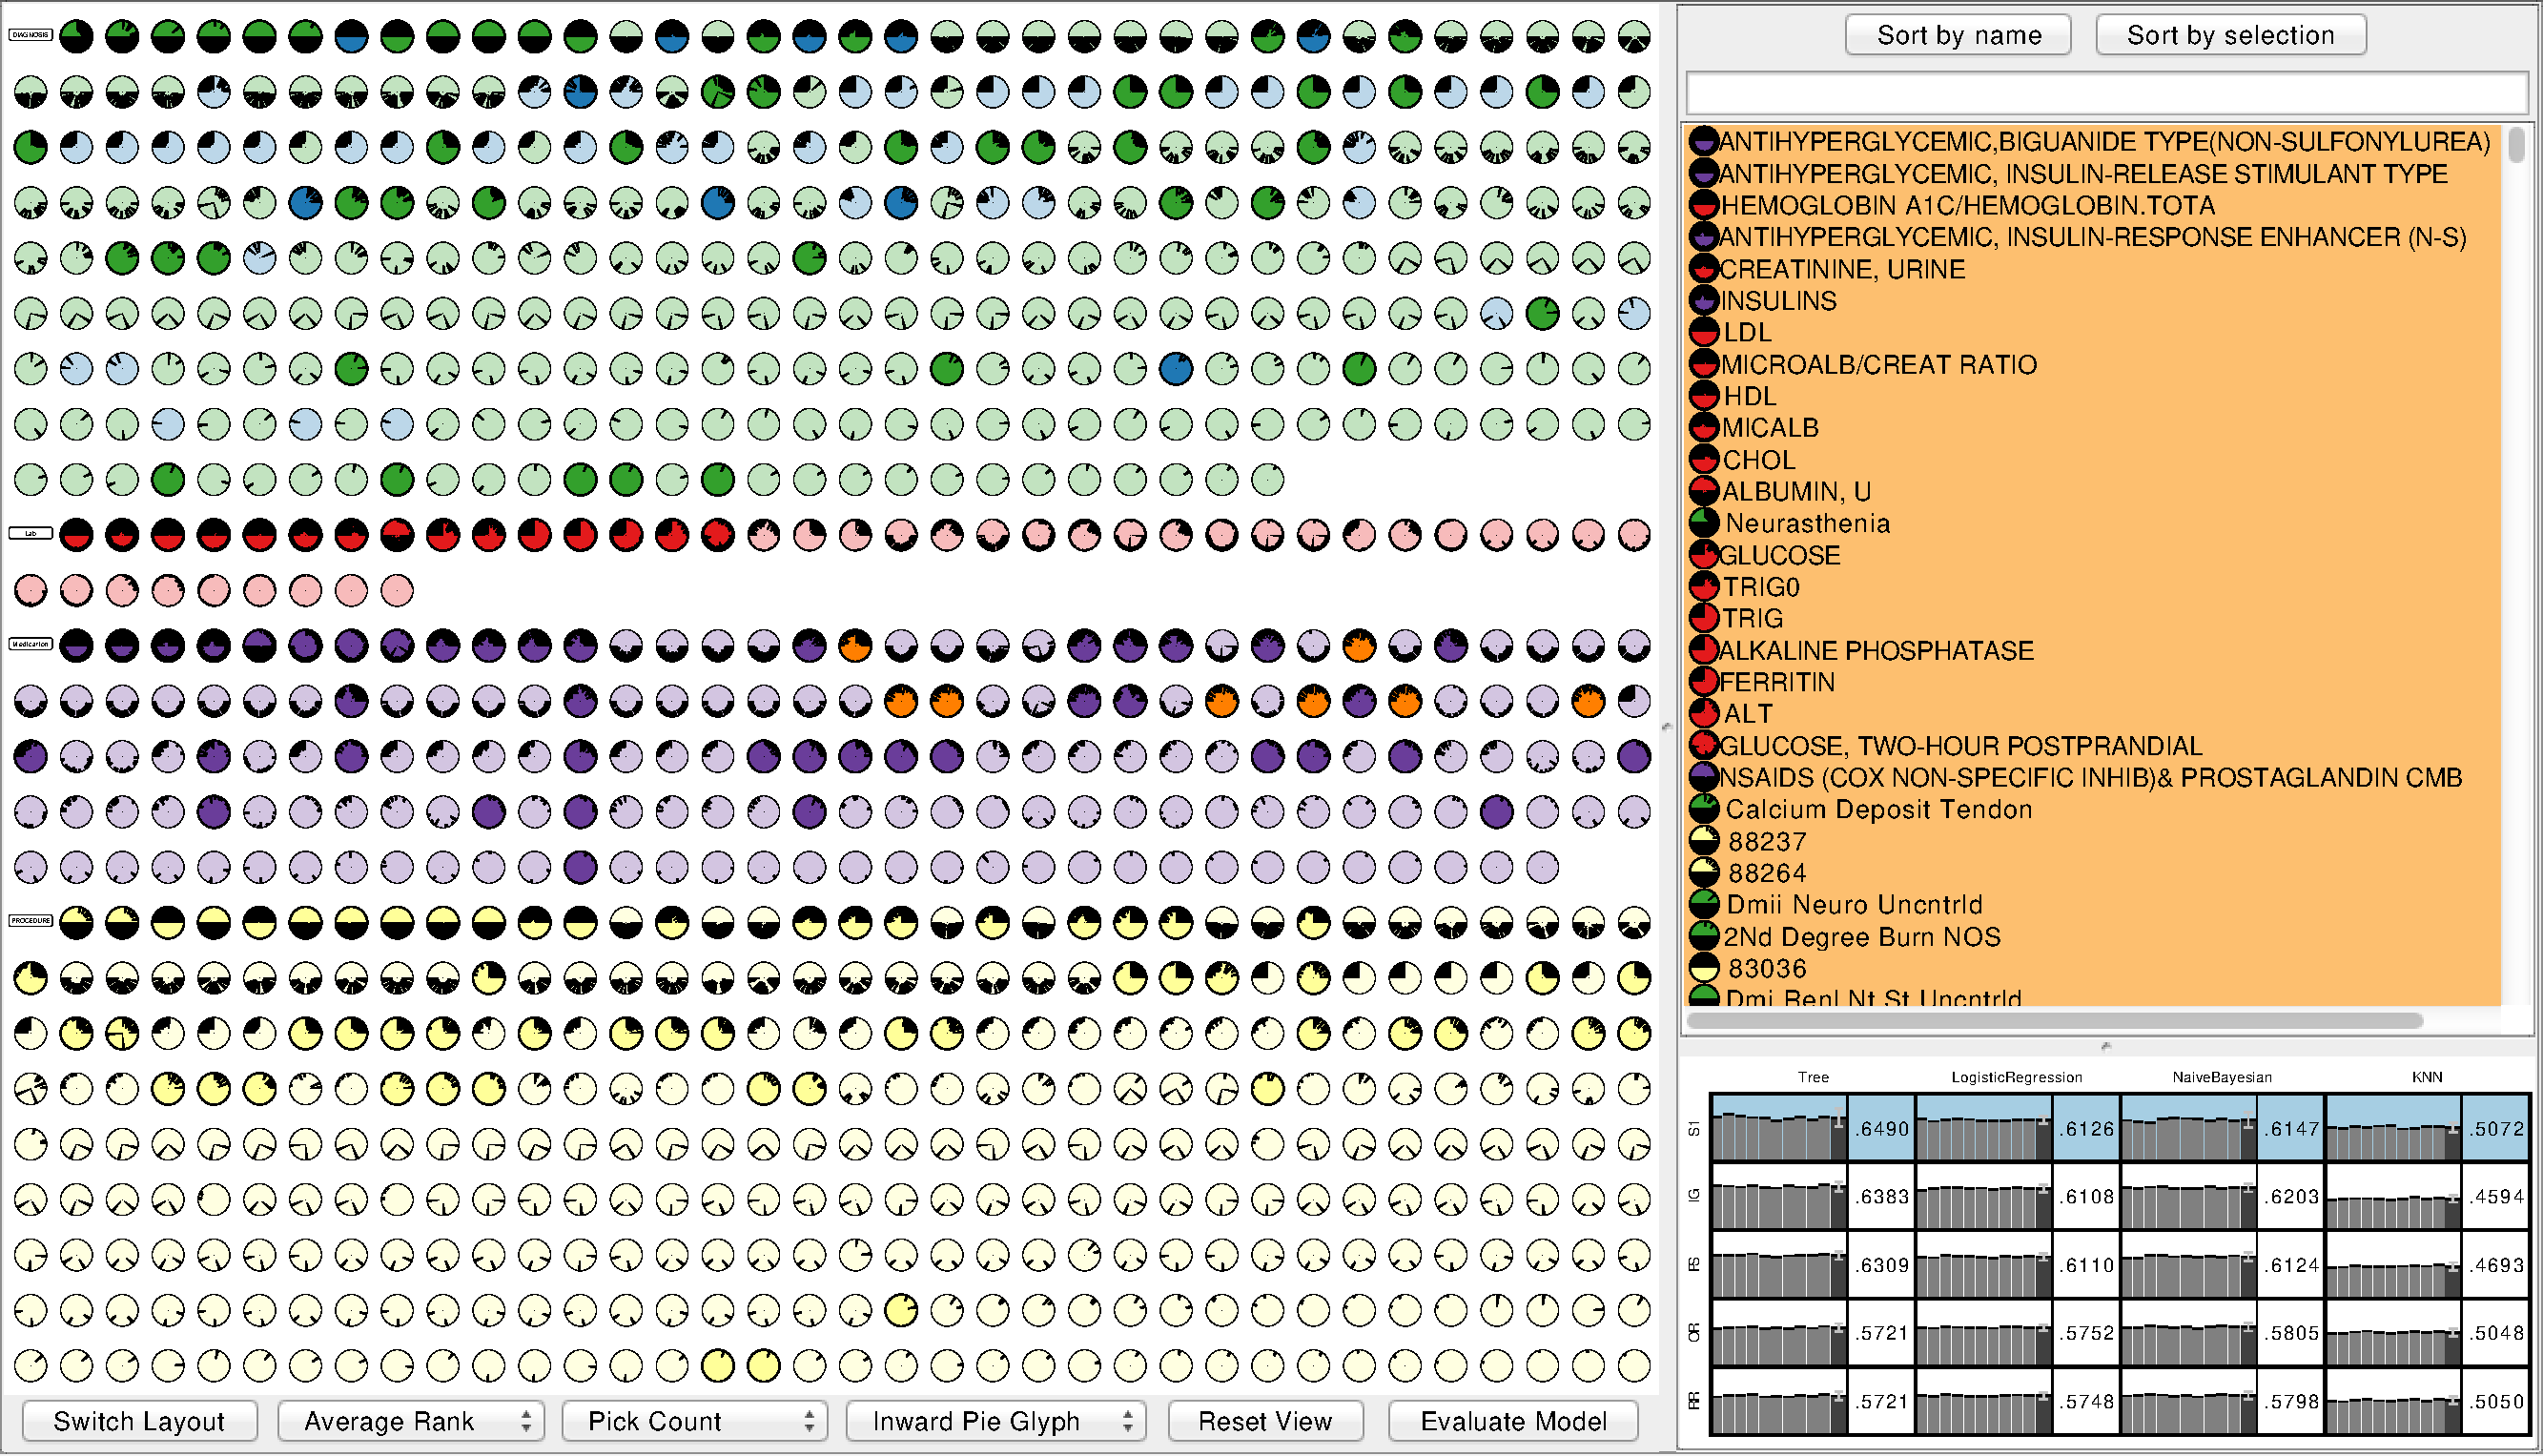
\includegraphics[width=\linewidth]{infuse/selection}
\caption{
\infuse's Interactive Model Builder allows users to select sets of features and measure its quality.
Selected feature glyphs are highlighted by saturating their color.  The List View is sorted to show the selected features by their importance.  After a user has made their selections, they can evaluate their model by clicking the ``Evaluate Model" button.  This adds a new blue row to the the Classifier View, showing the results of the evaluation for the user-defined model.
}
\label{fig:selection}
\end{figure}

\subsection{Interactive Model Builder}
\label{sec:imb}

One of the most important aspects of \infuse is that in addition to allowing the comparison of models, it also enables the creation of new models based on insights.
Users can select features for model building in a variety of ways.  They can select all of the features from existing models by clicking on a model in the Classifier View.  This will highlight and select all of the features that were used in the model.  Users can then augment these lists, or start from an empty set, by selecting individual features when clicking on them in the Feature or List view.  In order to select multiple features, a lasso selection technique is available in the Ranked and Scatterplot layouts.

After a feature set has been collected, \infuse can automatically evaluate the predictive performance of the user-defined model. By clicking the ``Evaluate Model" button,
%(\adam{Would be better named as "Evaluate Selected Model" but may not be worth doing new screenshots})
the new model is scored across all cross-validation folds and classifiers, and the results are added in the Classifier panel as a new blue row.  In the example in Figure~\ref{fig:selection}, the user-defined model out-performed the automated models and it is ranked at the top of the Classifier View.
Note that the user created model does not appear in the glyph.
This is due to the fact that the user does not need to rank the
features in order to obtain a classification result and that the feature
set is equal for all cross-validation folds.

% In every part of the system, features can be selected.
% Entire groups of features can be selected via clicking on
% a model in the classifier view or by using lasso selection in
% the feature view.
% The selection of single features can be changed by clicking in
% either the feature or list view.
% The set of selected features can eventually be used
% to create a new model.
% By clicking on the rightmost button at the bottom
% the area under curve values for the new model are computed
% and a new row is inserted at the correct position in the classifier view
% (see Figure~\ref{fig:selection}).
% This is helpful for an expert to verify whether a manually created set of
% features performs better than the automatically created sets.

% !TEX root = ../featureselection.tex

\section{Case Study}
Throughout our paper, we have used a running example of a team
of clinical researchers using predictive modeling to
classify patients at high risk of developing diabetes.
In this section, we describe how \infuse has led to a variety
of insights when exploring the features of the models.

\begin{figure*}[ht]
\centering
\resizebox{0.9\linewidth}{!}{%
\begin{tikzpicture}
\newcommand*{\imgwidth}{3.7cm}
\newcommand*{\boxsize}{0.437cm}
\newcommand*{\boxpos}{(.295, -.18)}
\newcommand*{\rightimagepos}{(4.8, 0)}
\newcommand*{\leftimagepos}{(0, 0)}
\node[inner sep=0pt] at \leftimagepos
    {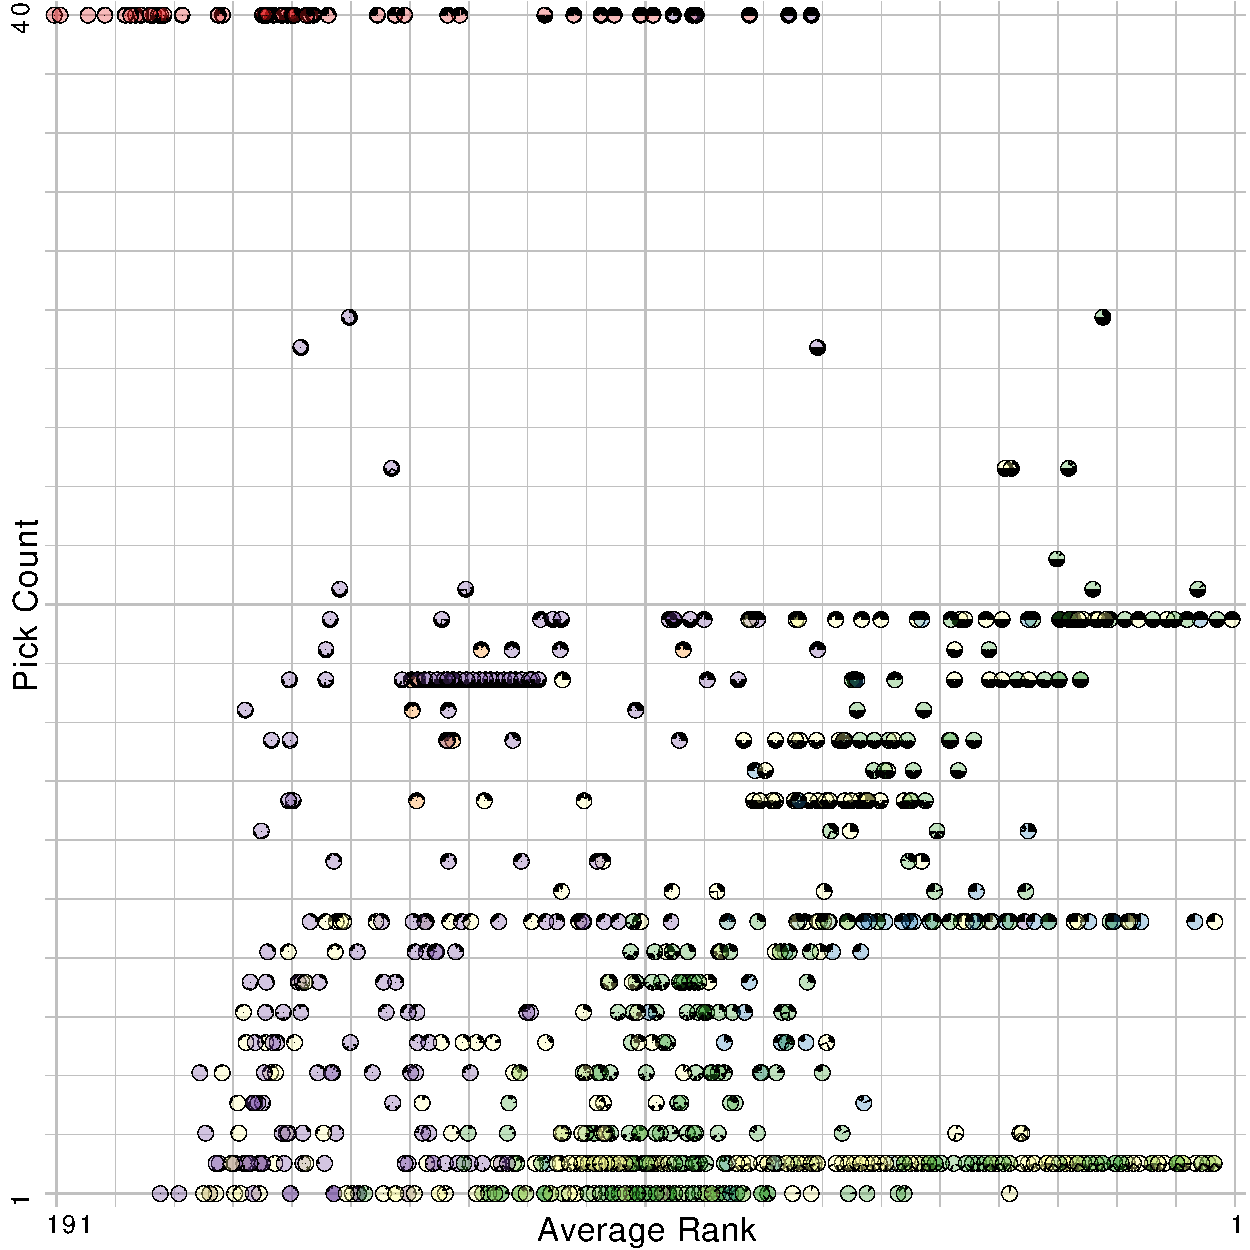
\includegraphics[width=\imgwidth]{infuse/ap}};
\node[inner sep=0pt] at \leftimagepos
    {\phantom{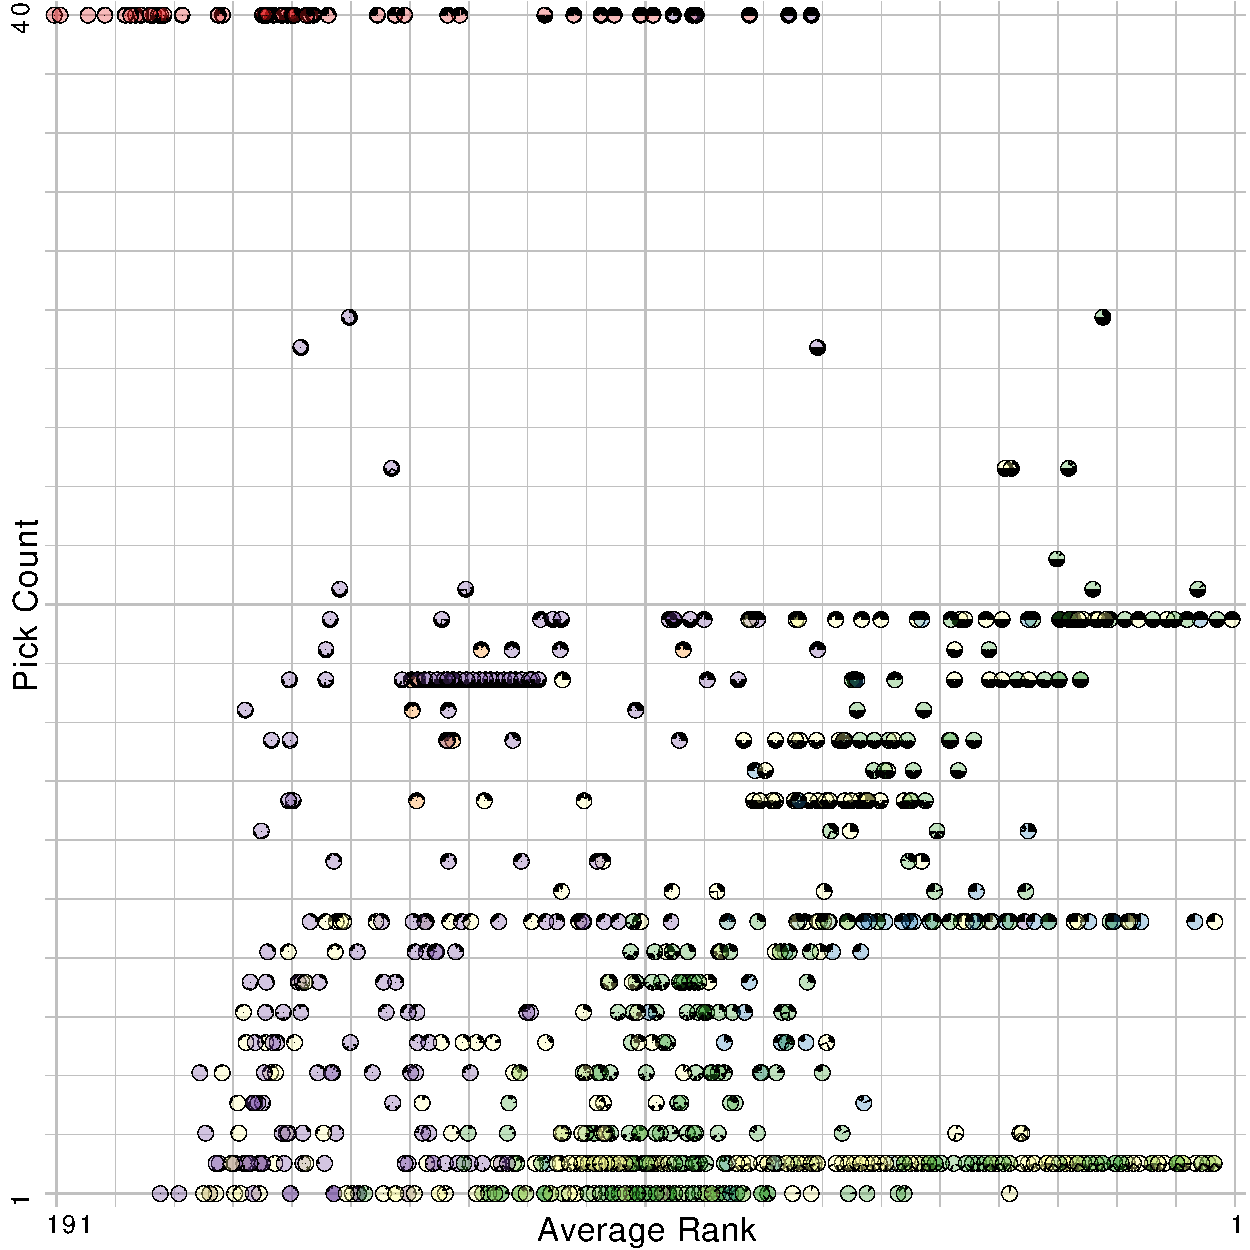
\includegraphics[width=\imgwidth]{infuse/ap}}};
\node[inner sep=2.5pt,very thick, text height=\boxsize] (zoom)
at \boxpos
    {\hspace*{\boxsize}};
\node[inner sep=-0.05pt] (lasso) at \rightimagepos
    {\phantom{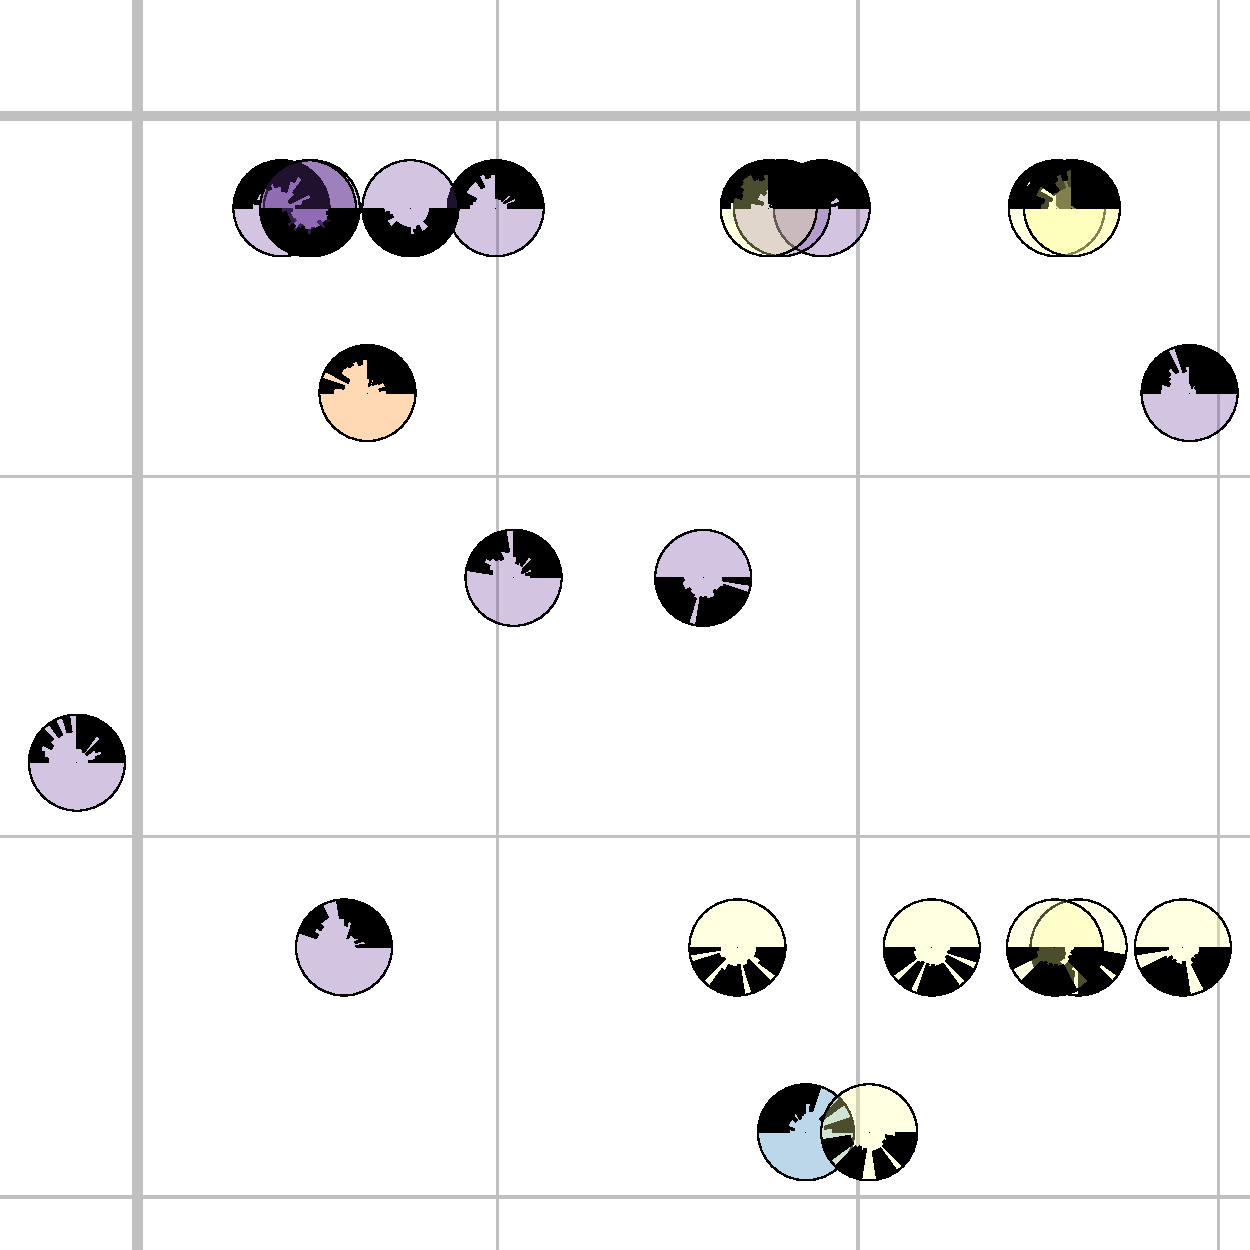
\includegraphics[width=\imgwidth]{infuse/lasso}}};
\draw (zoom.north west) -- (lasso.north west);
\draw (zoom.south west) -- (lasso.south west);
\draw (zoom.north east) -- (lasso.north east);
\draw (zoom.south east) -- (lasso.south east);
\node[very thick, draw=red!90, text height=\boxsize]
at \boxpos {\hspace*{\boxsize}};
\node[inner sep=0pt, very thick] at \rightimagepos
    {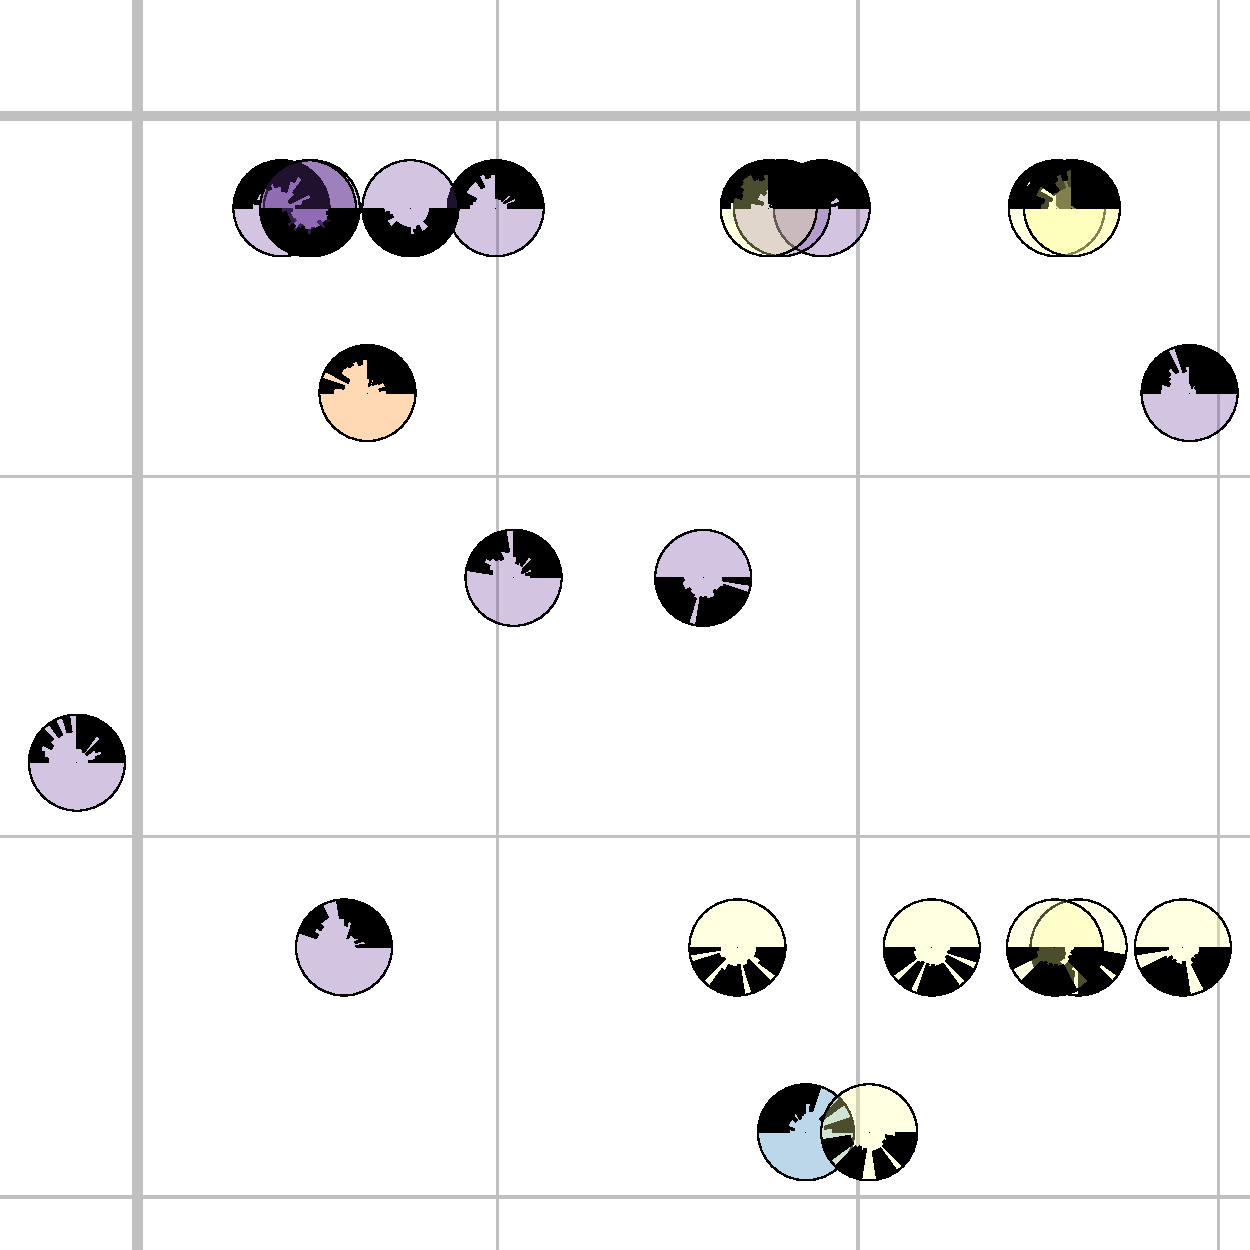
\includegraphics[width=\imgwidth]{infuse/lasso}};
\node[inner sep=0pt, very thick, draw=red!90] at \rightimagepos
    {\phantom{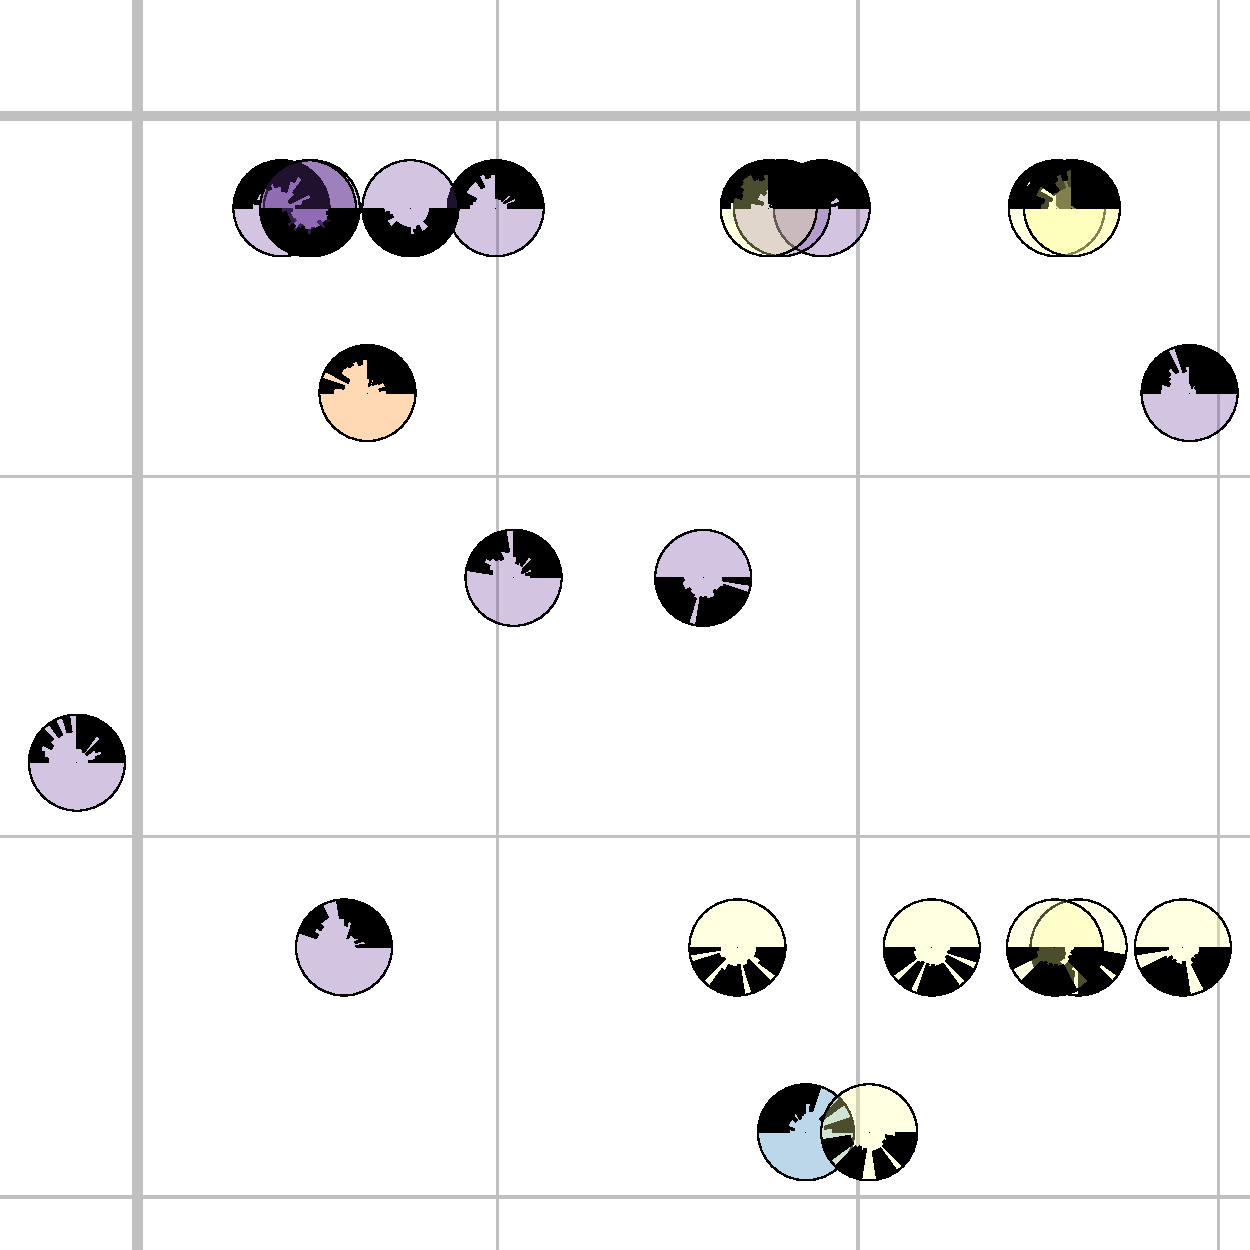
\includegraphics[width=\imgwidth]{infuse/lasso}}};
\end{tikzpicture}%
}
\caption[The scatter-plot view allows users to compare multiple types of rankings.]{
The scatter-plot view allows users to compare multiple types of rankings.  In the case study, users became curious of the medication features that were chosen by only half of the models.  When reviewing these medications with domain experts, it became clear that features picked by the upper-half algorithms were as clinically significant as those picked by the bottom-half.  This indicates that merging results from feature selection algorithms makes sense for this predictive model.
}
\label{fig:usecase2}
\end{figure*}

\subsection{Insight 1: Data issues}
When the clinical researchers learned of \infuse's capabilities
to compare multiple feature selection algorithms, they decided to
expand their pipeline's feature selection algorithms from 2 to 4.
The team has used Information Gain and Fisher Score extensively
in prior work, and typically uses these same techniques due
to their familiarity and past success.
Nonetheless, the diabetes data set introduced in Section \ref{sec:running_example} was new to them, and they were unsure which techniques would be the most appropriate. So, they asked their technologists to implement two new techniques: Odds Ratio and Relative Risk.

After all four algorithms were available, they executed their modeling pipeline
using \textit{PARAMO} \cite{paramo} and connected the results to \infuse.
Instantly, the team was surprised at the patterns that the visualization made evident.
The visualization indicated that there seemed to be little agreement between their two
old algorithms, and their two new algorithms for the best features.
The glyphs clearly indicated that many of the features were
highly ranked by two of the four feature selection algorithms,
and unranked by the other two, resulting in glyphs resembling alternating half-circles,
as shown in Figure~\ref{fig:usecase1}.
The team was quick to note that the resulting accuracy across
all four models were not significantly different,
so this non-overlap would have probably gone unnoticed if the
team just looked at resulting predictive scores at the
end of the pipeline as they typically do.

As \infuse gave them the opportunity to
examine multiple algorithms at the feature-level, they were curious as
to why this trend of non-overlapping feature rankings occurred.
They investigated the scores associated with each feature rank
and noticed that many of the features had scores
of $\infty$ from the Relative Risk algorithm.
It turned out there was a bug within the Relative Risk implementation where a
divide by zero error could happen if a feature did not occur
in any of the control patients.  After fixing this bug, they noticed that much of the non-overlap still was evident.  Looking more closely at the algorithms provided a
reason why the two new algorithms behave very differently:  they realized that both of the new algorithms only look at the presence and absence of the feature between the case and controls,
and do not pay attention to the feature values in any other way (e.g. distribution of values).
This is in contrast to the Fisher Score and Information Gain algorithms that take
the actual feature values into account.  This means that for features that are present in both case
and control groups in the same proportion, there is no discrimination value.

One of the team members mentioned, ``Each feature selection algorithm captures different types of information.  \infuse allows you to see what the effect of that information is being captured and gives you insight into the robustness of your predictive model."

As different algorithms will make sense for different purposes depending on the dataset and goals, \infuse provides an ability to inspect the features and determine
which algorithms produce ranked sets of domain-relevant features.

\subsection{Insight 2: Clinically relevant features}
After the data issues were solved, the researchers began investigating
the content of the predictive features.
Using the scatterplot view,
they inspected all of the medications that were ranked by all
feature selection algorithms and folds and found that they
were \textit{antihyperglycemic} medications, which are common treatments to lower the blood sugar of diabetes patients, and made clinical sense to be ranked high.

However, looking towards the center of the scatterplot,
where the features are only ranked by half of the algorithms and folds,
the researchers noticed a cluster of medications that
had half-circle patterns like those described above. This region is highlighted in Figure~\ref{fig:usecase2}. By mouse-hovering these features to read their names, it became clear that those ranked high by the upper-half of the circle (Information Gain and Fisher Score) were as clinically relevant and similar as those ranked by the bottom-half algorithms (Relative Risk and Odds Ratio). This provided feedback that in predictive modeling it is not safe to assume that one single feature selection algorithm is able to detect all possible interesting features and also that having a system like \infuse allows them to build a much richer picture of what kind of feature sets may lead to effective modeling. Without such a tool they would be restricted at evaluating one single algorithm at a time or, at best, restricting the comparison to a small number of features.

%it's not just certain feature selection algorithms that do not a better job overall, but instead might led themselves to finding certain features of various types -- all of which might strengthen the model.

After interacting with the system one of the team members said, ``\textit{If you just use one feature selection algorithm, you're only getting certain types of features. \infuse gives you a guide to what you might be missing. Using a combination type approach [with the Interactive Model Builder] will lead to stronger predictive models.}"

The clinical team is now going to re-think their strategy about how they
build predictive models and may consider using features by merging top
ranked features from different types of feature selection algorithms.
The researchers are convinced that by merging features, in addition
to the interactive model building capability, their predictive models will be improved.

\begin{figure}[t]
\centering
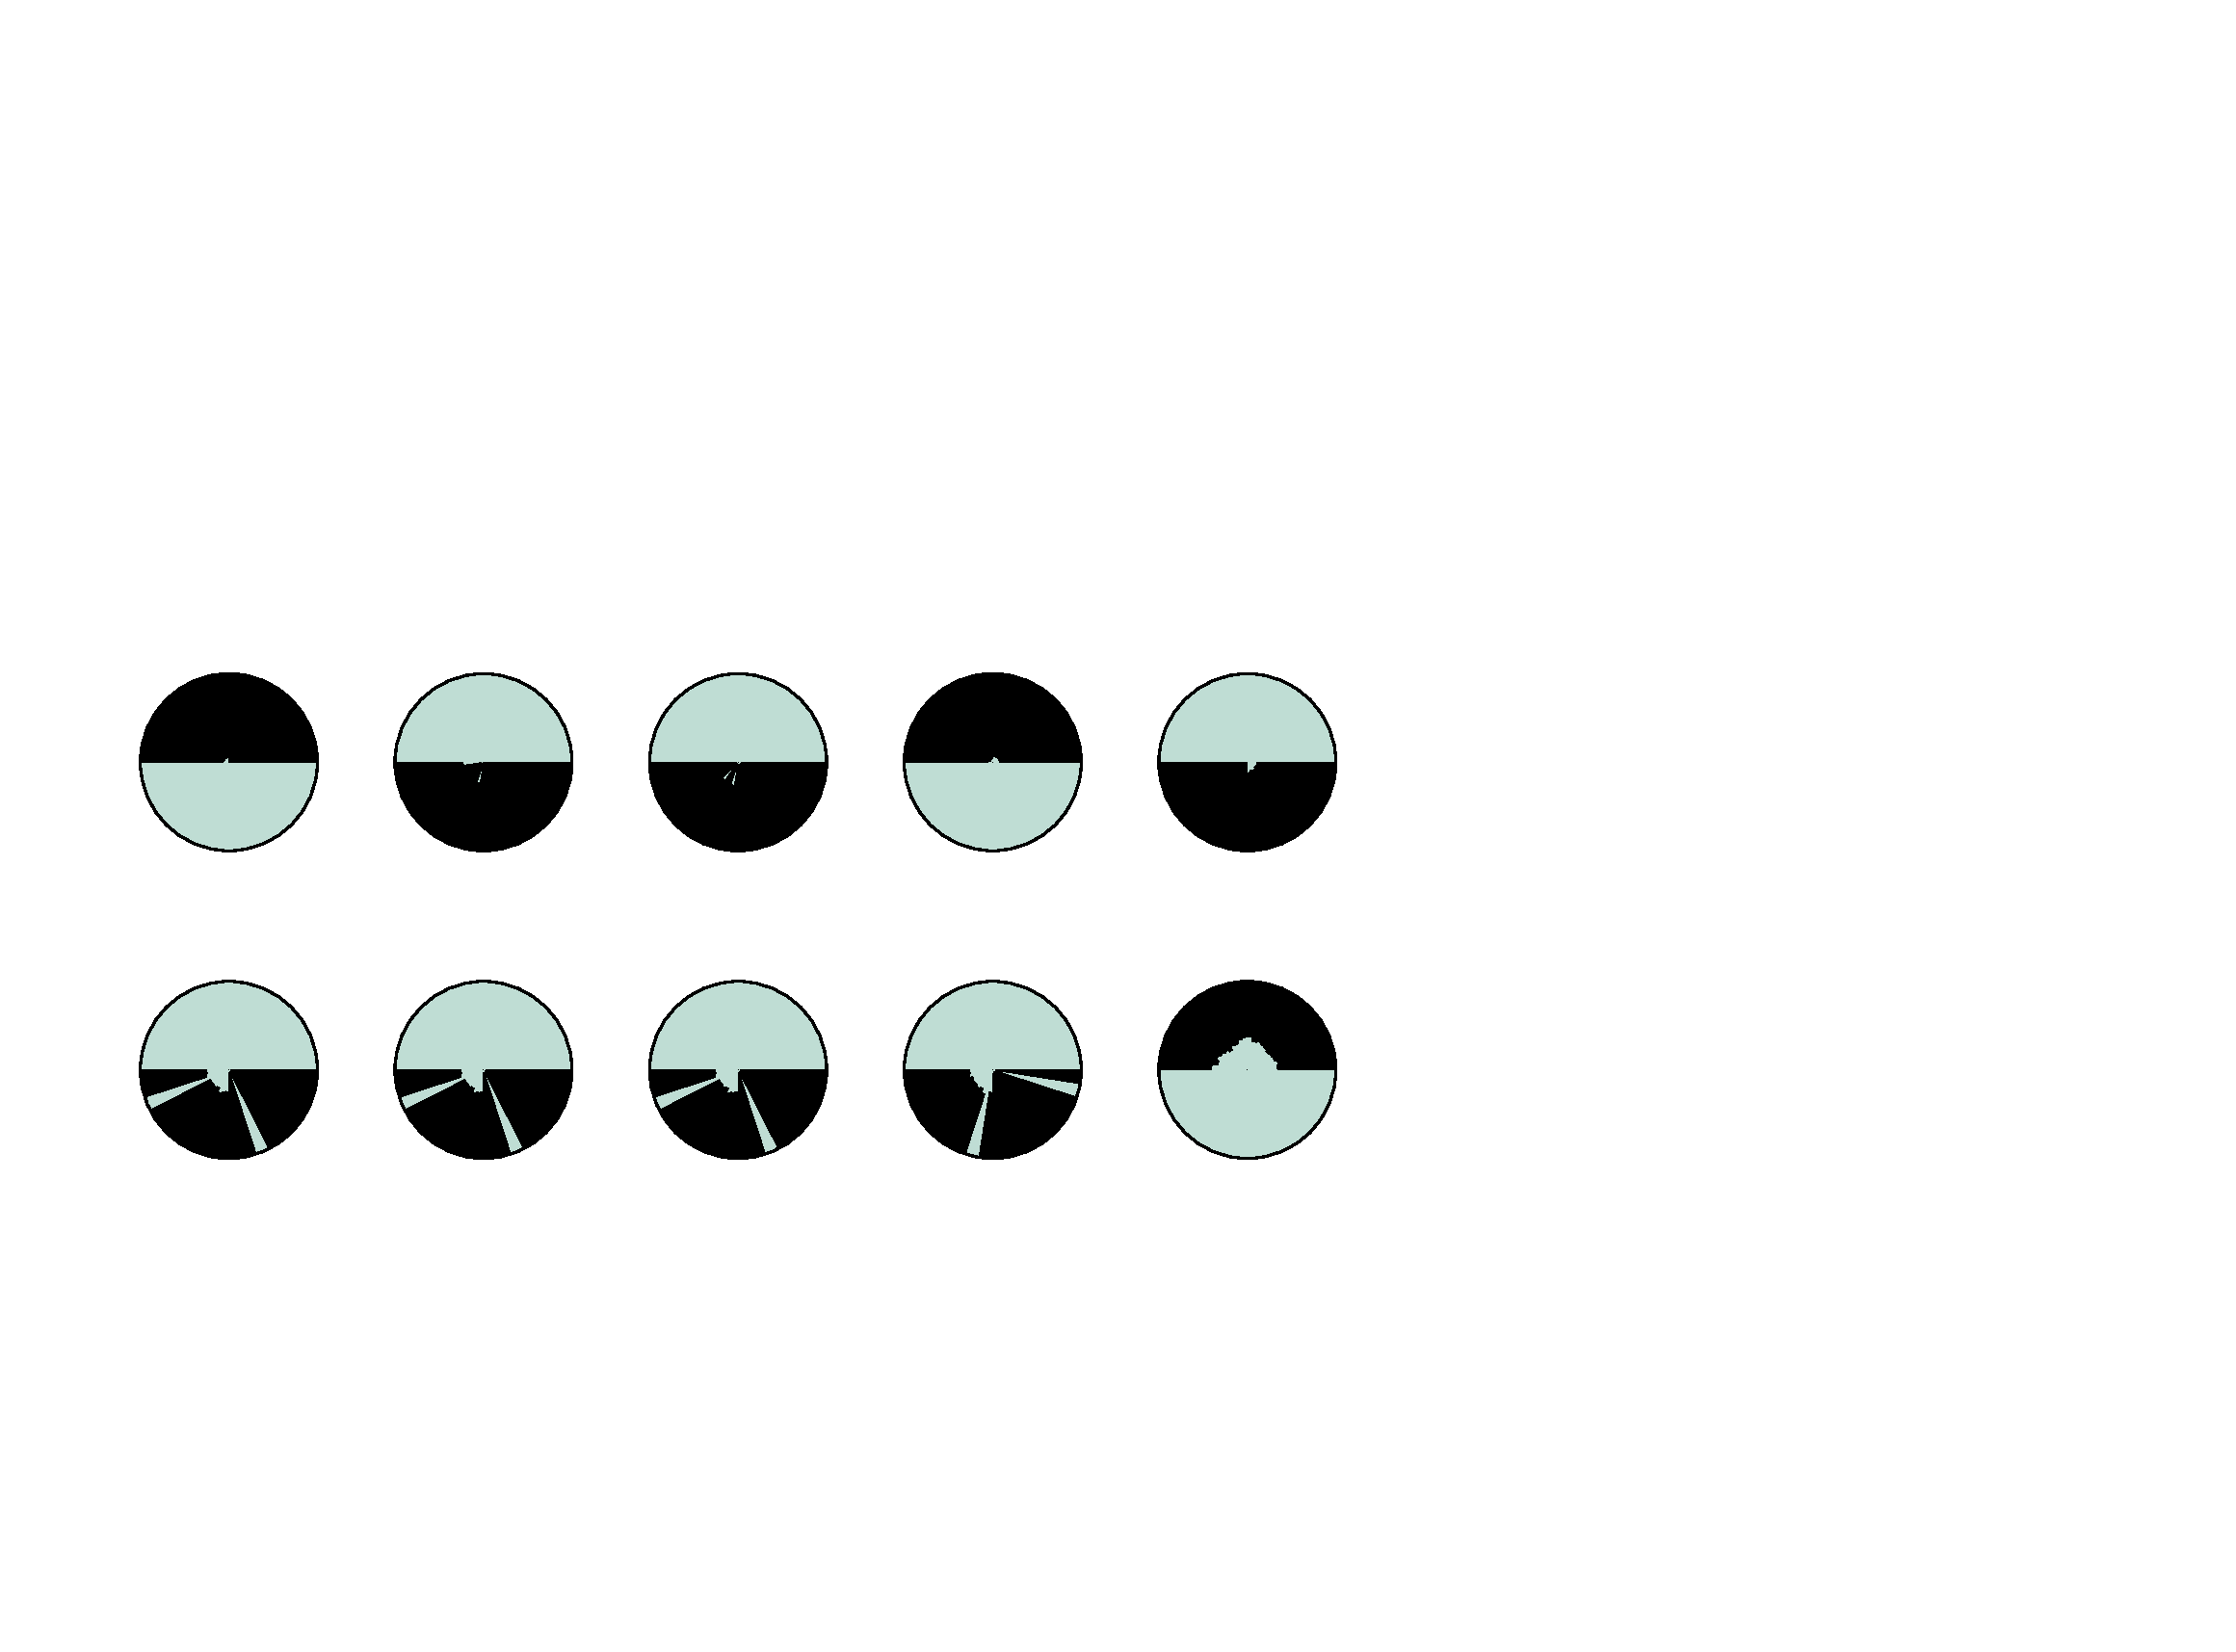
\includegraphics[width=\linewidth]{infuse/usecase1b}
\caption[The clinical researchers found an interesting pattern among
the glyphs.]{
The clinical researchers found an interesting pattern among
the glyphs indicating non-overlap of feature selection algorithm results.
These features were highly ranked by 2 of the 4 feature algorithms,
and unranked by the other 2, resulting in glyphs that resemble half-circles.
}
\label{fig:usecase1}
\end{figure}

% !TEX root = ../featureselection.tex

\section{Future Work and Conclusion}
There remains a great deal of research to further improve the analytical process of predictive modelers. \infuse only focuses on the feature selection step of predictive modeling. Each of the other steps would benefit from a visual interface to explore and parameterize the pipeline as well.

The search capabilities also have room for improvement by allowing more complex queries like features with a given range of ranks or features picked by a given algorithm, which would ease the task of finding relevant features for a user.
Also, expanding the range of the search box to filter also in the Feature View may reduce the number of overlapping glyphs in the scatterplot view.
Other clutter reduction techniques could also be available to users, such as a semantic zooming overlap resolution strategy that can jitter glyphs that overlap when the view is zoomed in.

Finally, to date, this tool has been used extensively for predictive modeling on clinical data.
However, \infuse was designed to be domain-independent and can easily be used for other domains in need of high-dimensional predictive modeling.  Our future work includes additional case studies in other domains to ensure the robustness of our tools.  This would also give the opportunity to explore the scalability of the design.  Typically, the number of cross-validation folds is not more than ten.  However, certain analysts may wish to compare a larger number of feature selection algorithms which would decrease the amount of space available per algorithm in the glyph.  While similarly-ranked features would still appear visually alike, it may become difficult to identify certain algorithms or folds without the help of interaction.  The overall number of features also plays a role in scalability concerns.

In conclusion, predictive modeling techniques are increasingly being used by data scientists to understand the probability of predicted outcomes.  We present \infuse, a tool that
lets users interactively create predictive models.  Typically, the predictive modeling pipeline leaves users out of the loop, and the algorithms operate as a black box.  By giving users the power to interact with the results of feature selection, cross validation folds, and classifiers, \infuse has shown promise to improve the predictive models of analysts.  We further demonstrated how our system can lead to important insights in a case study involving clinical researchers predicting patient outcomes from electronic medical records.


%% if specified like this the section will be ommitted in review mode
% \acknowledgments{
The authors thank Kenney Ng for providing
his expertise in predictive modeling.
The authors also thank the anonymous healthcare institution
who provided the data for the clinical researchers experiments.
% }


% \bibliographystyle{abbrvnat}
% \bibliography{progressive_vis}
% \end{document}


\section{General Discussion}
\infuse~\cite{infuse} explored the viability of the popular method of using feature importance measures to understand model behavior.
Even though there is no \emph{direct} influence from the model itself feature importance gives valuable insights due to its role in feature selection for the model and the similarity of its computation and the model's construction.
However, our experiments showed that there is little consensus between different feature importance algorithms, even though equal model performances were achieved.
This is likely due to redundancies in features in the input data but shows that those methods are not able to properly point out those occurrences.
Furthermore, it also shows that those feature importance methods are too far from the actual model to gain sufficiently strong insights into the model's behavior.
This result encouraged used to explore techniques of model dependent feature importance metrics, such as \prospector described in the next Chapter.

% \section{SeekAView: An Intelligent Dimensionality Reduction Strategy for Navigating HD Data Spaces}
% \label{sec:SeekAView}
% % \begin{figure}[t]
\centering
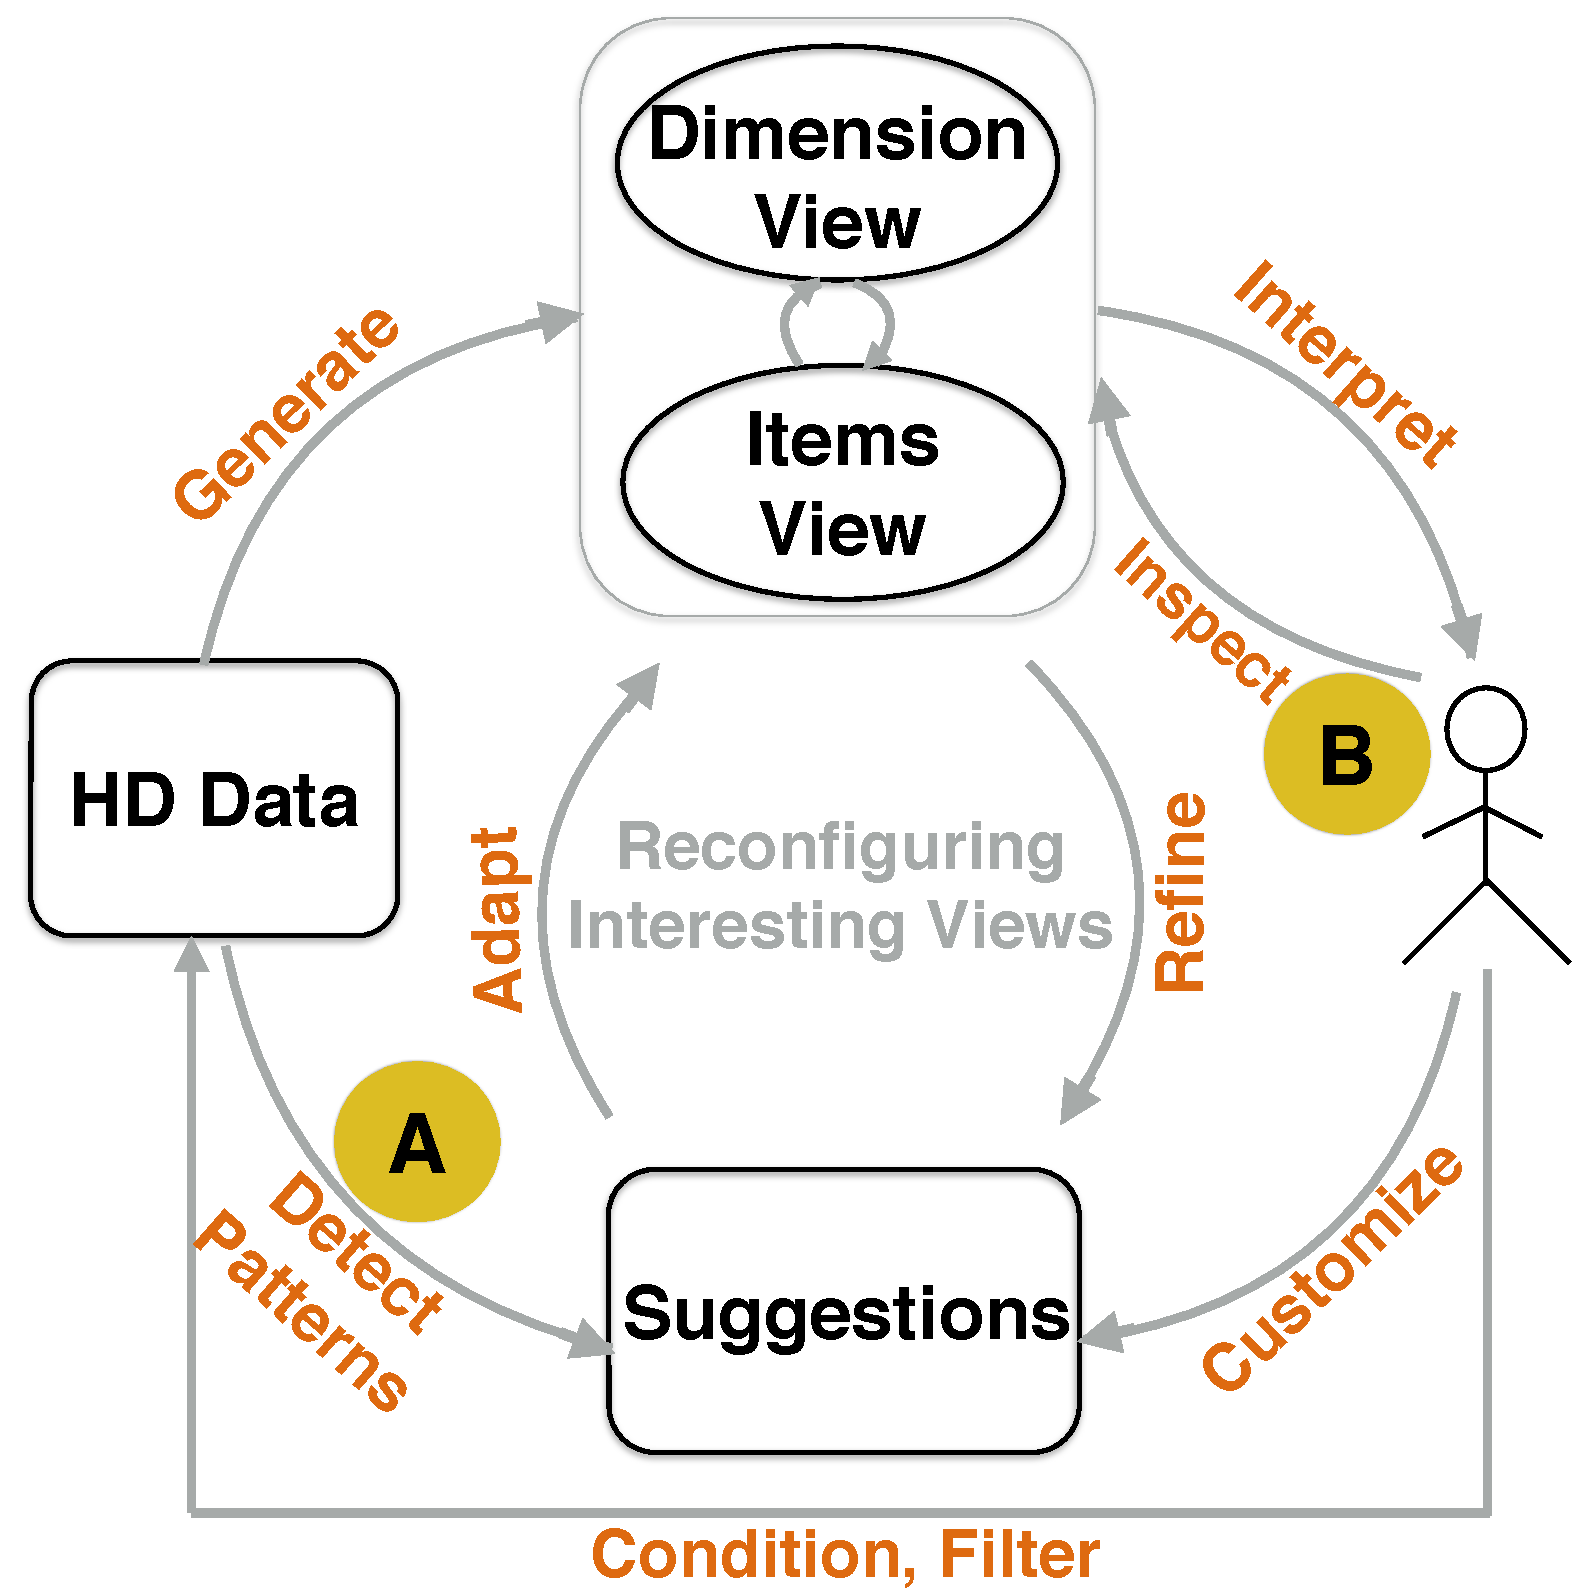
\includegraphics[width=0.8\columnwidth]{figs/seekaview/workflow}
\caption{Framework for guided reconfiguration of interesting views out of high-dimensional data: A tight integration of system generated suggestions with analysts' actions leads to flexibility in having multiple starting points of analyses~(A and B), and transparency in being able to refine the suggestions and adapt both dimension and item space interactively.
}
\label{figs:seekaview_workflow}
\end{figure} \figref{figs:seekaview_workflow}
% Dealing with the curse of dimensionality is a key challenge in high-dimensional data visualization. We present \textbf{SeekAView} to address three main gaps in the existing research literature. First, automated methods like dimensionality reduction or clustering suffer from a lack of transparency in letting analysts interact with their outputs in real-time to suit their exploration strategies. The results often suffer from a lack of interpretability, especially for domain experts not trained in statistics and machine learning. Second, exploratory visualization techniques like scatter plots or parallel coordinates suffer from a lack of visual scalability: it is difficult to present a coherent overview of interesting combinations of dimensions. Third, the existing techniques do not provide a flexible workflow that allows for multiple perspectives into the analysis process by automatically detecting and suggesting potentially interesting subspaces.
% In \textbf{SeekAView} we address these issues using suggestion based visual exploration of interesting patterns for building and refining multidimensional subspaces. Compared to the state-of-the-art in subspace search and visualization methods, we achieve higher transparency in showing not only the results of the algorithms, but also interesting dimensions calibrated against different metrics. We integrate a visually scalable design space with an iterative workflow guiding the analysts by choosing the starting points and letting them slice and dice through the data to find interesting subspaces and detect correlations, clusters, and outliers. We present two usage scenarios for demonstrating how \textbf{SeekAView} can be applied in real-world data analysis scenarios.

% \begin{figure}[ht!]
\centering
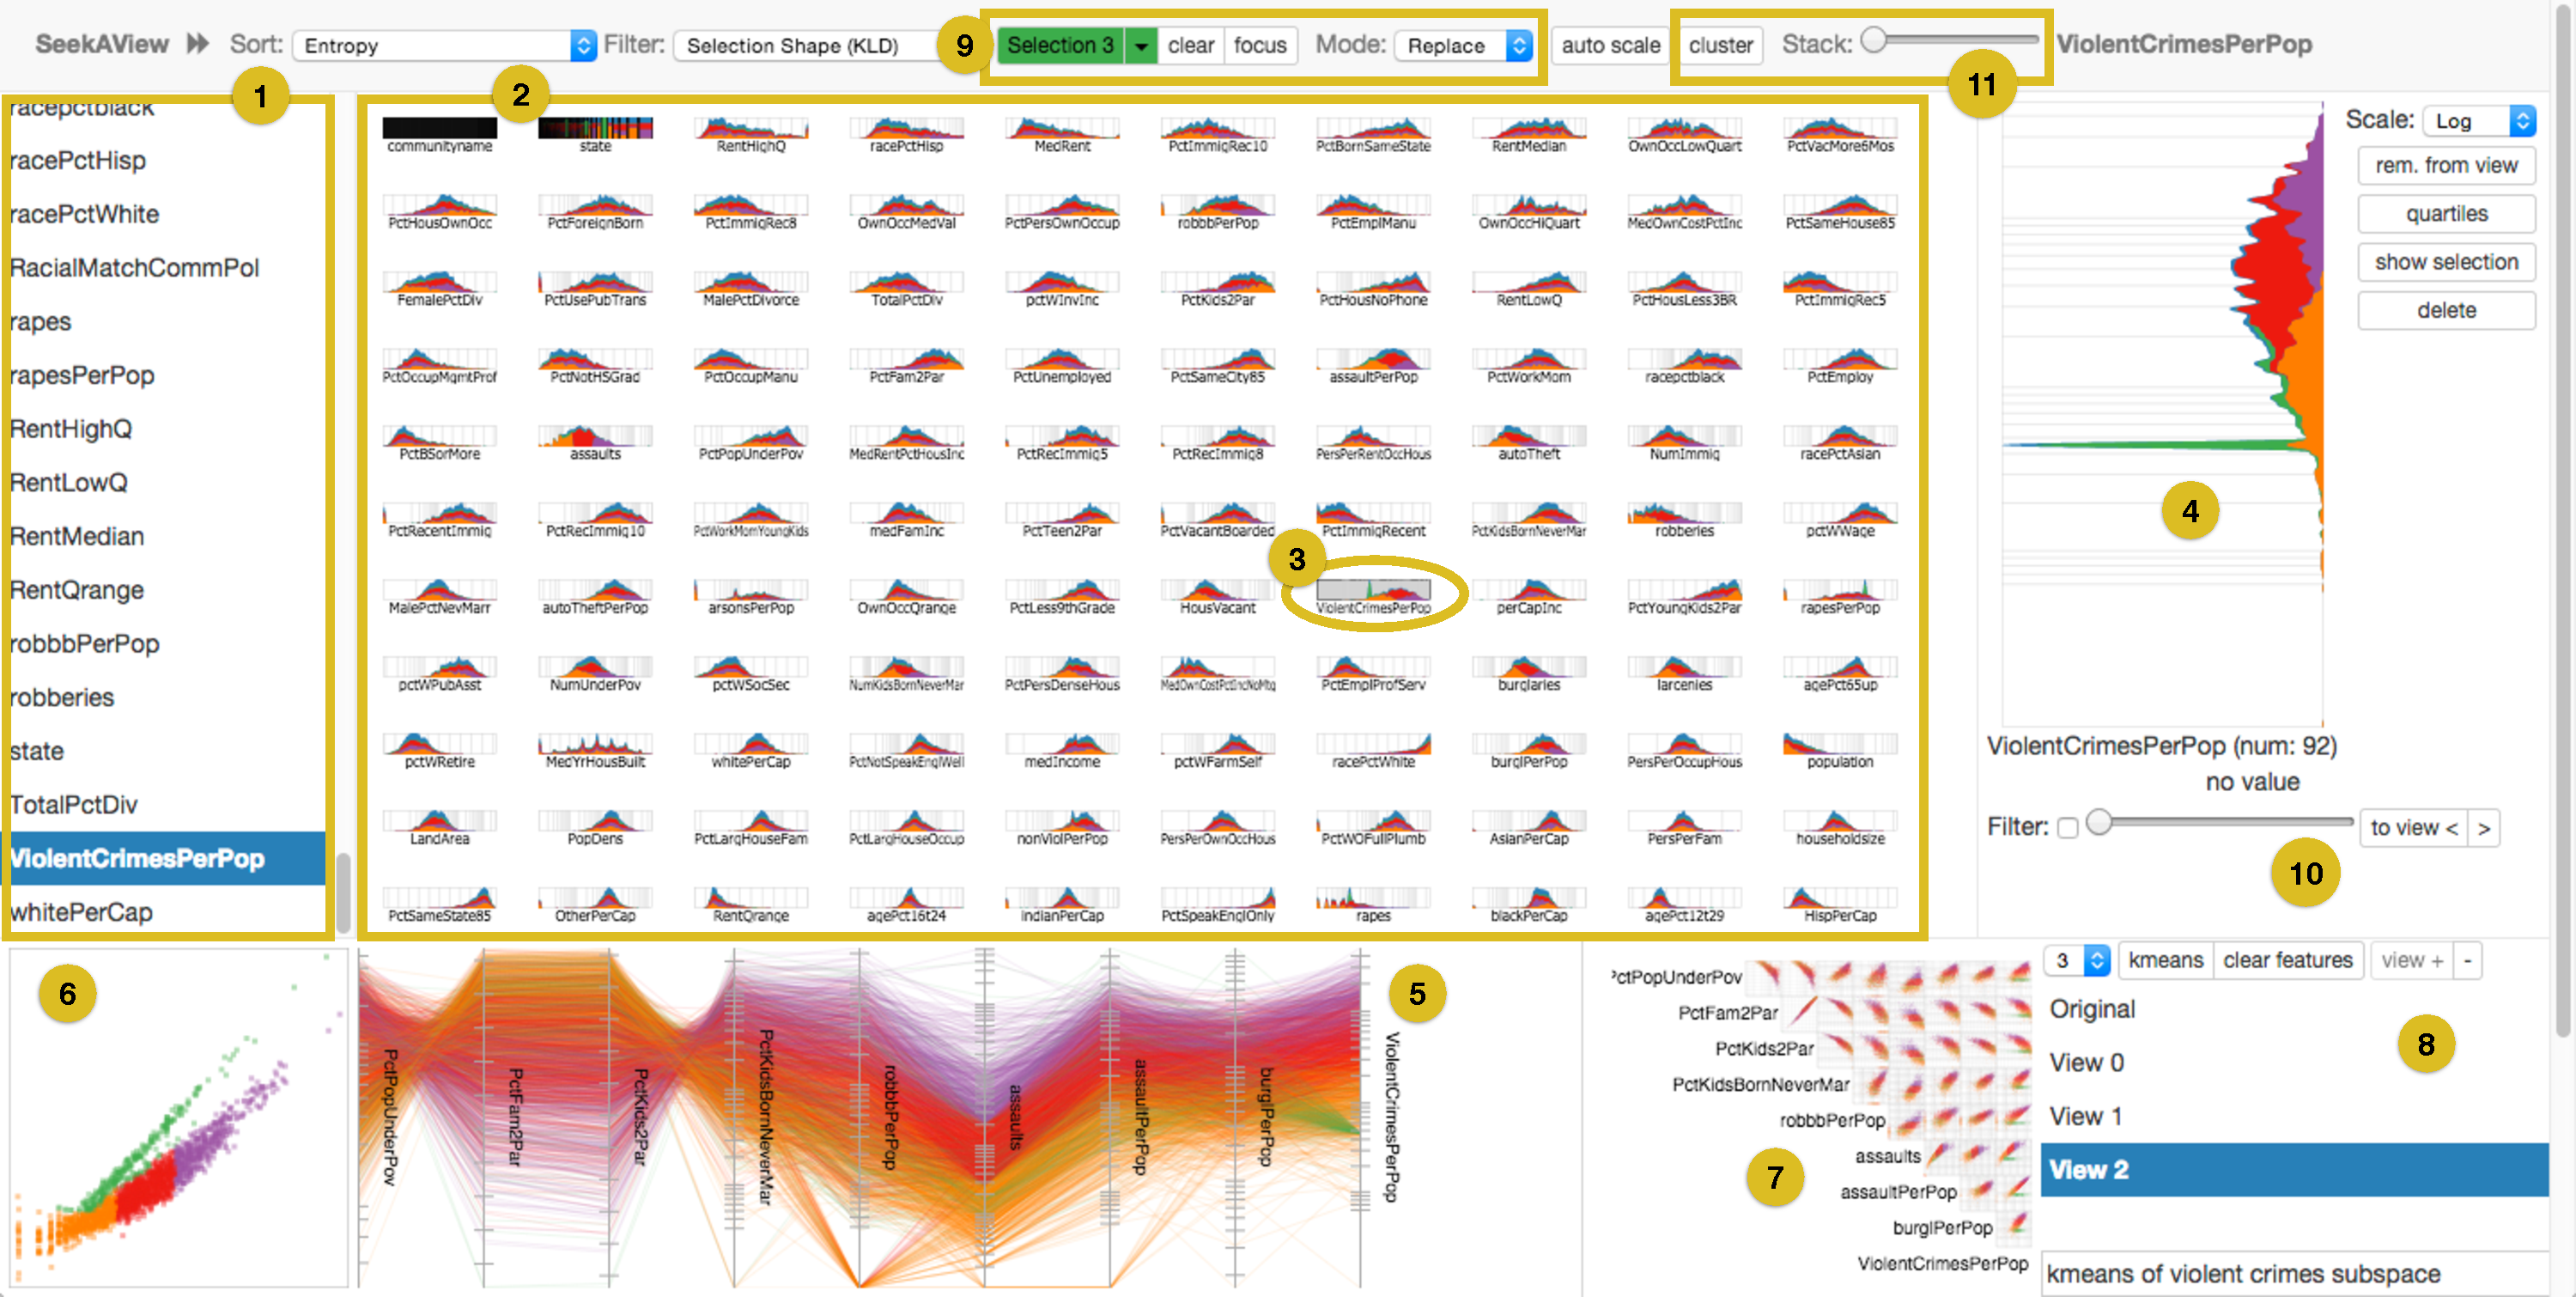
\includegraphics[width=0.9\linewidth]{figs/seekaview/overview}
\caption{
The user interface of \textbf{SeekAView}.
}
\label{figs:seekaview_overview}
\end{figure}

% The user interface of \textbf{SeekAView} can be seen in \figref{figs:seekaview_overview}.
% (1) is the list of all dimensions while (2) shows them as small multiple frequency plots. Selected dimensions are high-lighted (3)
% and shown in the target plot (4). The current multivariate view can be seen in the multidimensional view panel consisting of parallel coordinates (5), a PCA scatter plot (6), and a scatter plot matrix (7). Views can be selected, created, removed, and annotated in the lower right (8).
% Manual brushing can be configured at the top (9).
% Subspace suggestions can be created with a one-to-many filter (10) or by computing subspace (``cluster") or dimension similarity (``stack") clusters (11).
% The current state is the end of the Communities and Crime case study finding dimensions related to ``Violent Crimes per Pop."
% and further clustering the item space.

% \textbf{SeekAView} has been published as \cite{seekaview}.

% \section{Patient-viz: Visual Inspection of Longitudinal Electronic Medical Records}
% \label{sec:Patient-viz}
% \begin{figure}[hb!]
\centering
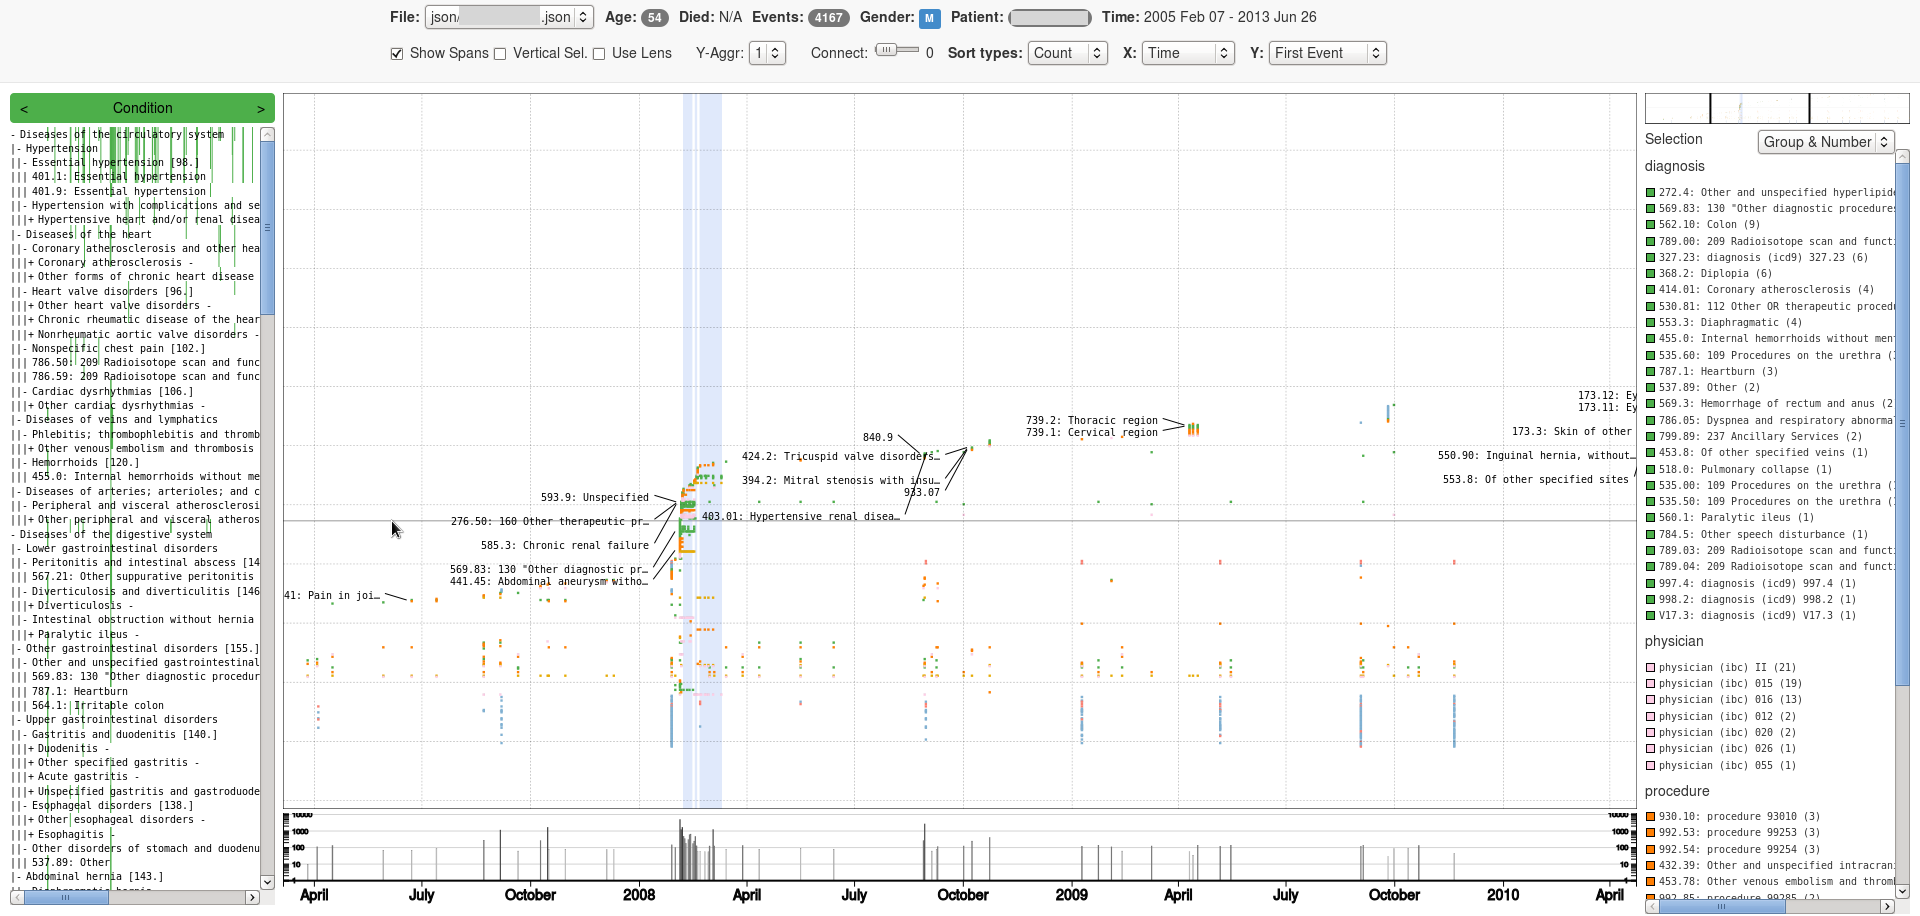
\includegraphics[width=0.9\linewidth]{figs/patientviz/p2-1_anon}
\caption{
The user interface of \textbf{Patient-viz}.
}
\label{figs:patientviz_overview}
\end{figure}

% Electronic medical records (EMRs) and administrative data contain a
% large amount of distinct events, like diagnoses, laboratory tests, \etc ,
% making it difficult to ``tell" the story of a patient.
% We propose \textbf{Patient-viz} to address this issue by using
% a visual representation of the data.
% This allows us to provide the large number of distinct event types
% and additional information like costs and hospital stays
% in a manageable form.
% Using both an anonymized public and an unaltered private dataset
% we explore the usefulness of our tool.

% Longitudinal studies and insurance claims data generate a large amount of
% electronic medical records (EMRs) and administrative data.
% This data contains a large number of distinct events throughout the
% observed time window of the life of patients.
% Understanding, interpreting, and finding relations in those records is a
% challenging task that is hard to achieve using a tabular
% or similar representation.
% Therefore, visualization is needed to \eg %help data scientists
% better understand predictive models built on top of the data,
% impact of comorbidities,
% progression of chronic diseases,
% or contributors of health care costs.

% Our proposed tool \textbf{Patient-viz} has a visually rich design aimed to
% make the huge amount of administrative data manageable for
% data scientists and medical doctors.
% The goal of the tool is to provide a quick overview of one patient
% which can be further explored to inspect detailed information.
% The input can be any temporal event
% data with a large number of differently typed events.
% We test our tool with online accessible semi-synthetic data provided by CMS~(\cite{cms_data}) and privately collected data from a major US insurance company.

% An overview of \textbf{Patient-viz} can be seen in \figref{figs:patientviz_overview}. The center shows events happening in the time-line
% with each row containing only events of the same type. At the bottom
% the cost of one day is shown.
% The top allows to change axes, the
% type aggregation level according to the CCS hiearchy~\cite{ccs},
% connect subsequent events,
% as well as change selection modes (vertical vs. horizontal),
% %if a lens should be used for labeling events,
% and shows general information about the patient.
% The lists left and right of the main view show all types and the current
% selection respectively.

% \textbf{Patient-viz} has been published as \cite{patientviz_poster} and \cite{patientviz_vahc}.

% \section{COQUITO: Supporting Iterative Cohort Construction with Visual Temporal Queries}
% \label{sec:COQUITO}
% \begin{figure}[b!]
\centering
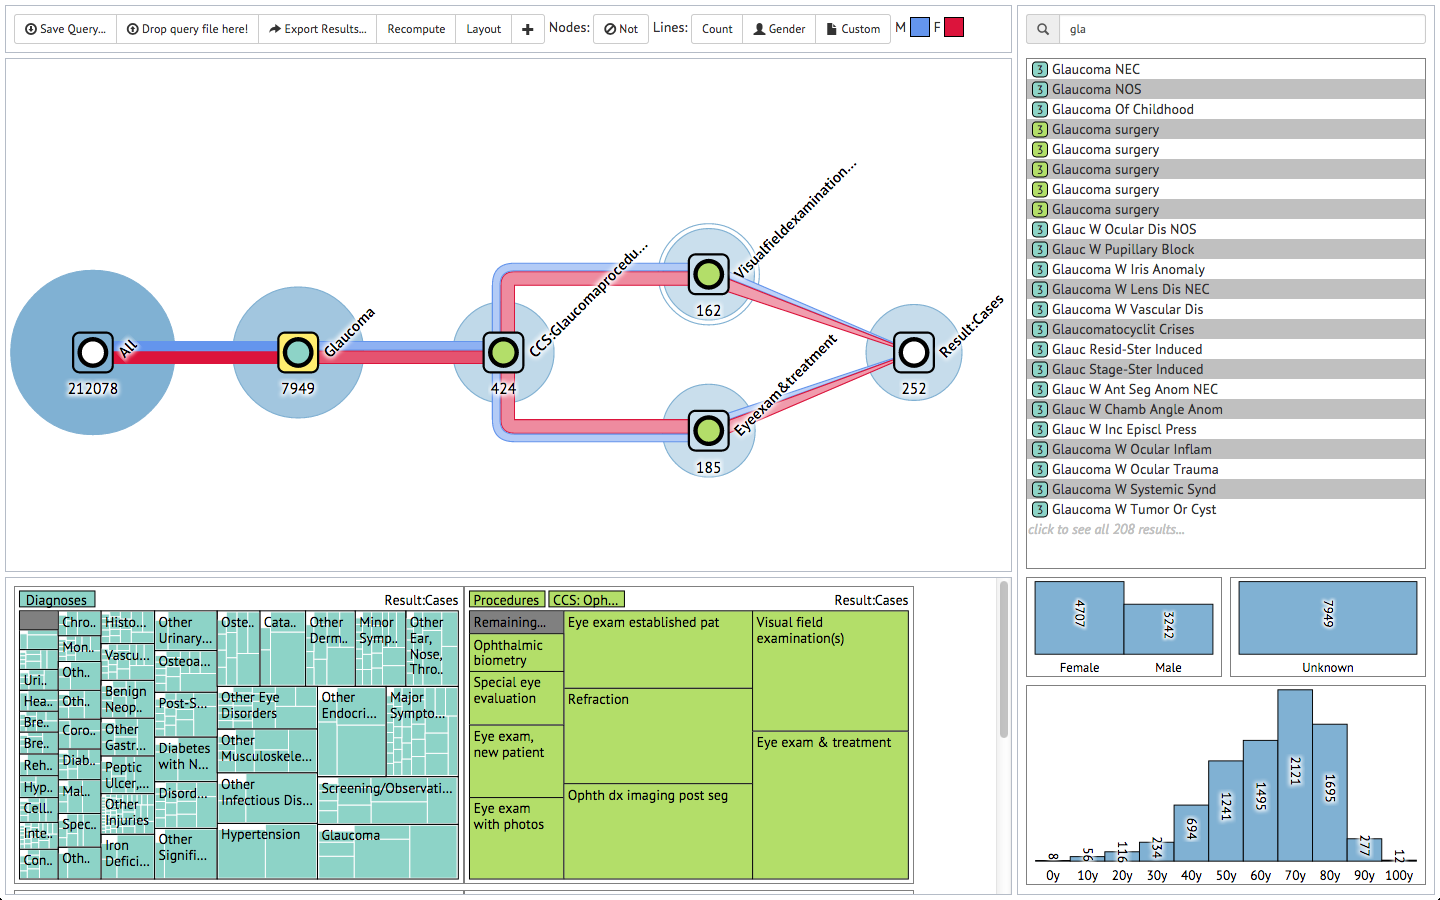
\includegraphics[width=0.9\linewidth]{figs/coquito/overview}
\caption{
The user interface of \textbf{COQUITO}.
}
\label{figs:coquito_overview}
\end{figure}%
% Many researchers across diverse disciplines aim to analyze the behavior of cohorts whose behaviors are recorded in large event databases.  However, extracting cohorts from databases is a difficult yet important step, often overlooked in many analytical solutions.  This is especially true when researchers wish to restrict their cohorts to exhibit a particular temporal pattern of interest.  In order to fill this gap, we designed \textbf{COQUITO}, a visual interface that assists users defining cohorts with temporal constraints.  \textbf{COQUITO} was designed to be comprehensible to domain experts with no preknowledge of database queries and also to encourage exploration.  We then demonstrate the utility of \textbf{COQUITO} via two case studies, involving medical and social media researchers.

% An overview of the \textbf{COQUITO} user interface can be seen in \figref{figs:coquito_overview}.  The center features the visual temporal query to define a cohort.  On the right, the search box is being used to locate additional event constraints.  Below the query, treemaps are shown to show the event distribution after the selected junction (``Glaucoma'' in yellow).  On the bottom right, demographics of the selected junction are also shown, including gender, ethnicity, and age distributions.

% \textbf{COQUITO} has been published as \cite{coquito}.
\chapter{Prospector}
\label{chap:prospector}
% \documentclass{sigchi}

% Use this command to override the default ACM copyright statement
% (e.g. for preprints).  Consult the conference website for the
% camera-ready copyright statement.

% \toappear{Permission to make digital or hard copies of all or part of this work for personal or classroom use is granted without fee provided that copies are not made or distributed for profit or commercial advantage and that copies bear this notice and the full citation on the first page. Copyrights for components of this work owned by others than the author(s) must be honored. Abstracting with credit is permitted. To copy otherwise, or republish, to post on servers or to redistribute to lists, requires prior specific permission and/or a fee. Request permissions from Permissions@acm.org. \\
% {\emph{CHI'16}}, May 07 - 12, 2016, San Jose, CA, USA \\
% Copyright is held by the owner/author(s). Publication rights licensed to ACM. \\
% ACM 978-1-4503-3362-7/16/05...\$15.00 \\
% DOI: \url{http://dx.doi.org/10.1145/2858036.2858529}}

%% EXAMPLE BEGIN -- HOW TO OVERRIDE THE DEFAULT COPYRIGHT STRIP -- (July 22, 2013 - Paul Baumann)
% \toappear{Permission to make digital or hard copies of all or part of this work for personal or classroom use is      granted without fee provided that copies are not made or distributed for profit or commercial advantage and that copies bear this notice and the full citation on the first page. Copyrights for components of this work owned by others than ACM must be honored. Abstracting with credit is permitted. To copy otherwise, or republish, to post on servers or to redistribute to lists, requires prior specific permission and/or a fee. Request permissions from permissions@acm.org. \\
% {\emph{CHI'14}}, April 26--May 1, 2014, Toronto, Canada. \\
% Copyright \copyright~2014 ACM ISBN/14/04...\$15.00. \\
% DOI string from ACM form confirmation}
%% EXAMPLE END -- HOW TO OVERRIDE THE DEFAULT COPYRIGHT STRIP -- (July 22, 2013 - Paul Baumann)

% Arabic page numbers for submission.  Remove this line to eliminate
% page numbers for the camera ready copy 

% \pagenumbering{arabic}

% \usepackage{acmcopyright}

% Load basic packages
% \usepackage{balance}  % to better equalize the last page
% \usepackage{graphicx} % for EPS, load graphicx instead 
%\usepackage[T1]{fontenc}
% \usepackage{txfonts}
% \usepackage{times}    % comment if you want LaTeX's default font
% \usepackage[pdftex]{hyperref}
% \usepackage{url}      % llt: nicely formatted URLs
% \usepackage[usenames,dvipsnames]{xcolor}
% \usepackage{color}
% \usepackage{textcomp}
% \usepackage{booktabs}
% \usepackage{ccicons}
% \usepackage{todonotes}
% \usepackage{xspace}
% \usepackage{amsmath}

% \newcommand{\joschi}[1]{\textcolor{RedOrange}{#1}}
% \newcommand{\adam}[1]{\textcolor{RedOrange}{#1}}

% \newcommand{\joschi}[1]{#1}
% \newcommand{\adam}[1]{#1}

% \newcommand{\eg}{\emph{e.g.}\xspace}
% \newcommand{\etal}{\emph{et~al.}\xspace}

% \newcommand{\prospector}{\emph{Prospector}\xspace}

% \DeclareMathOperator*{\argmin}{arg\,min}
% \DeclareMathOperator*{\argmax}{arg\,max}

% llt: Define a global style for URLs, rather that the default one
% \makeatletter
% \def\url@leostyle{%
%   \@ifundefined{selectfont}{\def\UrlFont{\sf}}{\def\UrlFont{\small\bf\ttfamily}}}
% \makeatother
% \urlstyle{leo}

% To make various LaTeX processors do the right thing with page size.
% \def\pprw{8.5in}
% \def\pprh{11in}
% \special{papersize=\pprw,\pprh}
% \setlength{\paperwidth}{\pprw}
% \setlength{\paperheight}{\pprh}
% \setlength{\pdfpagewidth}{\pprw}
% \setlength{\pdfpageheight}{\pprh}

% Make sure hyperref comes last of your loaded packages, to give it a
% fighting chance of not being over-written, since its job is to
% redefine many LaTeX commands.
% \definecolor{linkColor}{RGB}{6,125,233}
% \hypersetup{%
%   pdftitle={SIGCHI Conference Proceedings Format},
%   pdfauthor={LaTeX},
%   pdfkeywords={SIGCHI, proceedings, archival format},
%   bookmarksnumbered,
%   pdfstartview={FitH},
%   colorlinks,
%   citecolor=black,
%   filecolor=black,
%   linkcolor=black,
%   urlcolor=linkColor,
%   breaklinks=true,
% }

% create a shortcut to typeset table headings
% \newcommand\tabhead[1]{\small\textbf{#1}}

% End of preamble. Here it comes the document.
% \begin{document}

% \CopyrightYear{2016} 
% \setcopyright{acmlicensed}
% \conferenceinfo{CHI'16,}{May 07 - 12, 2016, San Jose, CA, USA}
% \isbn{978-1-4503-3362-7/16/05}\acmPrice{\$15.00}
% \doi{http://dx.doi.org/10.1145/2858036.2858529}

% \title{Interacting with Predictions: Visual Inspection of Black-box Machine Learning Models}

% \numberofauthors{3}

% \author{%
%   \alignauthor{Josua Krause\\
%     \affaddr{New York\\University}\\
%     \affaddr{New York, NY, USA}\\
%     \email{josua.krause@nyu.edu}}\\
%   \alignauthor{Adam Perer\\
%     \affaddr{IBM T.J. Watson\\Research Center}\\
%     \affaddr{Yorktown Heights, NY, USA}\\
%     \email{adam.perer@us.ibm.com}}\\
%   \alignauthor{Kenney Ng\\
%      \affaddr{IBM T.J. Watson\\Research Center}\\
%     \affaddr{Yorktown Heights, NY, USA}\\
%     \email{kenney.ng@us.ibm.com}}\\
% }
% \maketitle

  % UPDATED---\today. Abstracts should be about 150 words and
  % are required.

%%  Understanding predictive models is a challenging task. Often feature importance
%% given by a model is only a rough estimate condensed into one number. Using
%% partial-dependence plots for input features we can visually gain a feeling of
%% how a model is influenced by a given feature. In order to achieve this we treat
%% our machine learning model as a black-box, change our input data slightly, and
%% show the changes of the prediction. Using this technique we gain interesting
%% insights into multiple machine learning models and in turn how to improve them.
%% Furthermore, in the domain of health-care analytics we also use this approach to
%% focus on a single patient. Doing this we can interactively explore how
%% influential features are for a patient. This local importance can be used to
%% identify actionable features where a small change of the patient's state can
%% lead to a significant change of the disease risk of this patient.

% kng: I reworded the abstract ... feel free to not use if you don't like it
\begin{quote}\textit{
Understanding predictive models, in terms of interpreting and identifying actionable
insights, is a challenging task.
Often the importance of a feature in a model is only a rough estimate
condensed into one number.  However, our research goes beyond these na\"ive estimates through the design and implementation of an interactive visual analytics system,
\prospector. By providing interactive partial dependence diagnostics, data scientists can understand how features affect the prediction overall.  In addition, our support for localized inspection allows data scientists to understand how and why specific datapoints are predicted as they are, as well as support for  tweaking feature values and seeing how the prediction responds.  Our system is then evaluated using a case study involving a team of data scientists improving predictive models for detecting the onset of diabetes from electronic medical records.
}\end{quote}
% Using partial-dependence plots provides a way to visualize how a model
% is influenced by a given feature.
% This is achieved by treating the machine learning model as a black-
% box, systematically changing the input data values, measuring and
% then showing the changes in the prediction score.
% Using this technique, insights into multiple machine learning models
% can be obtained which can then in turn be used to improve them.
% Furthermore, in the domain of health-care analytics, this approach can
% be used to focus on a single patient. Specifically, one can
% interactively explore how influential different features are for an
% individual patient. This local importance can be used to identify
% actionable features where a small change in the patient’s state can
% lead to a significant change in the patient's predicted risk.

\begin{contributions}{How can partial dependence be leveraged to gain diagnostic insights into machine learning models?}
\item The partial dependence based feature importance score allows to effectively detect model errors.
\item Detectable errors include: over-fitting, under-fitting, errors caused by imputation, and incorrect cause-effect relationships.
\item Localized inspections help to understand the how and why of specific instance predictions by finding locally impactful features.
\end{contributions}

\begin{quote}
\textit{Josua Krause, Adam Perer, Kenney Ng}
\end{quote}

% \keywords{interactive machine learning; predictive modeling; partial dependence; %\joschi{sensitivity analysis;}
% visual analytics; model visualization}

% \category{H.5.m.}{Information Interfaces and Presentation
%   (e.g. HCI)}{Miscellaneous}
   % \category{See
  % \url{http://acm.org/about/class/1998/} for the full list of ACM
  % classifiers. This section is required.}{}{}

% !TEX root = ../prospector.tex

% \section{Introduction}

In the era of data-driven analytics, there is growing demand to generate and deploy predictive models in a variety of domains so that the patterns unearthed from massive amounts of data can be leveraged
% for the greater good.
and converted into actionable insights.
Predictive modeling is defined as the process of developing a mathematical tool or model that generates an accurate prediction \cite{kuhn2013applied}.  As an example, in health care, if one can model the data characteristics of patients who will likely develop Diabetes, health care institutions could deploy such a model on their patient databases, and automatically flag high risk patients to clinicians to make sure they are being treated appropriately.  However, building such models on noisy, real-world data is quite challenging.  

Data scientists often turn to machine learning, where the goal is to create predictive models based on information automatically learned from data with ground truth.  However, these machine learning techniques are often black-boxes and may be selected based only on performance metrics such as high accuracy scores, and not necessarily based on the interpretability and actionable insights of the model.  There has recently been a variety of techniques to inject humans-in-the-loop when building predictive models based on machine learning, from interactive training \cite{amershi15} to interactive feature selection \cite{infuse}.  However, interactive systems to effectively assess and evaluate the interpretability and actionable insights of a predictive model that go beyond simple accuracy metrics is still lacking.  We believe bringing humans into the loop at this stage can possibly lead to better models and consequently improved outcomes when the models are deployed.

Our research aims to support data scientists to go beyond judging predictive models solely based on their accuracy scores by also including model interpretability and actionable insights.  Towards this goal, we developed \prospector, a novel visual analytics system designed to help analysts better understand  predictive models.  \prospector leverages the concept of partial dependence, a diagnostic technique that was designed to communicate how features affect the prediction, and makes this technique fully interactive.  \prospector also supports localized inspection, so users can understand why certain data results in a specific prediction, and even lets users hypothesize new data by tweaking values and seeing how the predictive model responds.  We also demonstrate, through a case study, how the system can lead to important insights for clinical researchers building models that try to predict patient outcomes based on electronic medical records.

Concretely, our contributions include:

\begin{itemize}
\item A design and implementation of an interactive visual analytics system,
\prospector, for assessing the interpretability and actionable insights of trained predictive models by supporting:
\begin{itemize}
    \item Interactive partial dependence diagnostics to understand how features affect the prediction overall. There are novel visual representations, sampling strategies, and support for comparing multiple models.
    \item Localized inspection to understand how and why specific instances are predicted as they are.  Users can interactively tweak feature values and see how the prediction responds, as well as find the most impactful features using a novel local feature importance metric.
  \end{itemize}
\item A case study of data scientists using
\prospector to improve predictive models for detecting the onset of Diabetes trained from electronic medical record data.
\end{itemize}

% \begin{itemize}
%   \item Machine learning algorithms increasingly being relied on in data science.
%   \item One such class of machine learning algorithms are predictive classifiers.
%   \item Predictive models offered judged by their accuracy score, and not necessarily by their components.
%   \item For those examining components, judgment is often done via naive importance weights
%   \item Our contribution is to go beyond these naive metrics to provide:
%   \begin{enumerate}
%     \item Partial Dependence.  Understand how features affect the prediction overall.  Leverage an existing diagnostic technique called partial dependence, but make it interactive/coordinated.
%     \item Localized Inspection.  How does the model affect specific data rows (patients).
%   \end{enumerate}
%   \item Deeper inspection of predictive models can help ensure the models are grounded in reality.
%   \item Help data scientists focus on determining actionable features (to go beyond prediction) e.g. focusing clinicians on features that may improve the patient's health, or focusing city managers on features that may lower crime.
% \end{itemize}

% Theme of 2016 conference is \#chi4good.  Play up how bringing humans in the loop for important domain predictions can possibly lead to better models and better outcomes.

% Two parts:
% 1. what are partial dependence plots good for? (global)
% its useful for inspecting and improving models.
% 2. how to use partial dependence for predicting single rows (local)
% its also useful as a local tool for understanding the impact of the model on specific data points.

% !TEX root = ../prospector.tex

\section{Motivation}

\input{prospector/ml_crash}

\subsection{Predictive Modeling in Health Care}

In order to make our contributions concrete, we utilize a motivating scenario that emerged from our case study.  The case study involves a team of five data scientists interested in using predictive modeling on a longitudinal database of electronic medical records. The research team has a background in health care analytics and their database contains 4,000 patients from a major hospital in the United States. The team is interested in building a predictive model to predict if a patient is at risk of developing Diabetes, a chronic disease of high blood sugar levels that may cause serious health complications.

\input{prospector/pd-explain}

The team of data scientists manages to develop a highly accurate predictive model for detecting patients at high risk of developing Diabetes.  They determine its effectiveness by measuring the common metrics used by predictive models (e.g., accuracy and AUC scores \cite{kuhn2013applied}).  They also followed the best practices of building predictive models.  They worked with clinical researchers to properly define cohorts of patients with Diabetes (cases) and matched patients without Diabetes (controls) by thoroughly searching through the electronic medical records.  They constructed features based on lab tests, diagnosis codes, procedures, demographics, and patient conditions from the records.  They used cross-validation to ensure their models were robust.  They used a variety of state-of-the-art feature selection methods to utilize the most informative features in the model while keeping it as generalizable as possible.  And they used a variety of effective classifiers to do the training and evaluation.  After trying various combinations of these techniques, the model with the highest accuracy metrics was selected and presented to the appropriate stakeholders at the health care institution.

Their stakeholders were impressed by the high accuracy scores of the model.  But when they asked the data scientists for more information about what was inside of the model, the reports only described the top features of the model and their associated ``importance" weights.  The stakeholders recognized many of the feature names, and it appeared to make clinical sense.  However, there were also some surprising ones that led to intellectual discussions.  But the stakeholders demanded to know more.  They wanted a clearer sense of how certain features impacted the prediction.  Furthermore, they wanted to understand how the values associated with the features (\eg, the results associated with lab tests) impacted the prediction.  They also were curious to interact with the model to test hypotheses about how the model would react to hypothetical patients of interest.  When confronted with these questions, the data scientists shrugged.  In the data scientist's defense, it is difficult to summarize and interpret complex models and there are few tools and techniques available to address the stakeholders' requests.  So now the stakeholders are faced with a hard decision:  do they deploy a predictive model in their institution that appears to have high accuracy but is also somewhat of a black-box?

Although this scenario is motivated by our case study, our other projects and interviews suggest these are not atypical requirements.  Our work is motivated to support the development of more comprehensible predictive models. 

\subsection{Partial Dependence}

\input{prospector/partial_dependence}

% !TEX root = ../prospector.tex

\section{Related Work}

\subsection{Motivation for Interpretability}
Modern machine learning algorithms are able to create more reliable and precise models
but they are increasingly complex and come with the price of being harder and harder to interpret (Breiman~\cite{breiman2001}).
This inverse relation of understandability versus expressiveness of a model introduces the need
to find ways to improve the interpretability of complex models to overcome this disadvantage.
Lim~\cite{Lim:2012:IUT:2518922} asks questions such as ``\emph{Why} did X happen?",
``\emph{Why} not Y?", ``\emph{What} happens \emph{if} I do Z?", and ``\emph{How} do I make X happen?"
to explain complex mechanisms like machine learning models.
Our system allows users to interactively ask and answer such questions.
Kulesza~\etal~\cite{Kulesza:2015:PED:2678025.2701399} use explanatory debugging by conveying how a model
came to its prediction in order to be able to correct mistakes.
On the other hand, Patel~\etal~\cite{DBLP:conf/ijcai/PatelDFKT11} use multiple classifiers
to better understand input data.
Steeg~and~Galstyan~\cite{NIPS2014_5580,steeg2015corex_theory} use total correlation to build
a hierarchy of features explaining their role in the data.

\subsection{Algorithm Specific Model Visualization}
In the past, research has primarily focused on understanding and interacting with specific machine learning algorithms.
Often the focus is on the internal weights of the trained models.
For Bayesian networks, showing probabilities of the nodes (Becker~\etal~\cite{Becker:2001:VSB:383784.383809}) and how the input is propagated (Correa~\etal~\cite{DBLP:journals/isci/MartinsONHC13})
has been used.
For Support Vector Machines,
projection techniques (Caragea~\etal~\cite{Caragea2001}) and
Nomograms (Jakulin~\etal~\cite{Jakulin:2005:NVS:1081870.1081886})
to see the ``cut" in the data points were utilized.
Visualizing and interpreting the graph of a neural network has also been used by Tzeng and Ma~\cite{Tzeng:2005:OTB}.
Kim~\etal~\cite{kim2014bayesian,kim2015MGM} introduce graphical models that allow for
interpretability of its features.
\cite{kim2015MGM} use a colored matrix of features by category to show distinguishable features computed by their model.
Caruana~\etal~\cite{Caruana:2015:IMH:2783258.2788613} use high-performance generalized additive models (GA$^2$Ms) that allows visual inspection of the influence of its input features on the outcome much like partial dependence.

\subsection{Model Result Visualization}
However, showing only internal, algorithm specific weights is often not enough.
Plate~\etal~\cite{DBLP:journals/neco/PlateBGB00} and Olden~\cite{citeulike:3733836} show how input features influence
the outcome of neural network classifications.
Xu~\etal~\cite{DBLP:journals/corr/XuBKCCSZB15} interprets
the graph of a neural network used for image classification to
retrieve which part of an image was responsible for a specific
classification result.
These techniques aim in the same direction as partial dependence but are limited to only neural networks.
They cannot be used to support the ability to compare different machine learning models across algorithms.

Having access to the internals of a machine learning algorithm also allows direct interaction with the models and to improve them on the fly.
BaobabView (van den Elzen and van Wijk~\cite{6102453}) offers interactive decision tree construction.
Steed~\etal~\cite{5332586,doi:10.1559/152304009788988314}
guides regression model creation by enhancing interaction
with the input data.
EnsembleMatrix (Talbot~\etal~\cite{Talbot:2009:EIV:1518701.1518895})
allows users to combine already computed classification models to
build ensemble models.
Some recent interactive machine learning tools \cite{
amershi15,
Amershi:2011:DEE:2046396.2046416,
Amershi:2012:RIM:2207676.2207680,
Amershi:2011:CHF:1978942.1978966,
Kapoor:2010:IOS:1753326.1753529,
kim2015scalable,
Leung2014710,
Mishra:2015:SAI:2700171.2791022,
export:141330})
are more algorithm agnostic, but depend on general
performance measures like confusion matrices,
area under ROC curve (AUC) measures,
result distribution of data points, and
feature weights according to model independent statistics.

Frank and Hall~\cite{frank2003} use 2D projections of the data to show %classification
results for multiple classification algorithms, as well as Rheingans and desJardins~\cite{885740} with self-organizing maps.

\subsection{Probing Models}
Partial dependence was proposed by Friedman~\cite{friedman2001} for analyzing
gradient boosting models and has since been used for other models as well (\eg Ehrlinger~\cite{ehrlinger2015} uses partial dependence to analyze the behavior of random forests
in the \emph{R} package \emph{ggRandomForests}).

Cortez and Embrechts~\cite{cortez2011opening,Cortez20131} and Kim~\etal~\cite{kim2014bayesian}
use sensitivity analysis to analyze and compare machine learning models of different algorithms.
Sensitivity analysis is similar to partial dependence except that it uses a few
base vectors (usually the mean, median, or quartiles of all observed values)
instead of computing the probabilities over all input points.
This method is faster than partial dependence but may miss critical details
about the prediction function especially if the function is strongly non-linear.

Goldstein~\etal~\cite{goldstein14} extends the idea of partial dependence by using
Individual Conditional Expectation (ICE) plots which show one line for each row of the input data.
We found, however, that this often clutters the plots too much and makes them harder to interpret.
We experimented further with showing standard deviations and quartiles of the partial dependence line
but discarded this approach since the spread of the partial dependence results is always expected to
be large unless one feature dominates the classification significantly and is able to solely change
the classification even for the furthest data points.

By not restricting ourselves to sampling only the observed input space, our approach on partial dependence
enables a deeper analysis of the machine learning model. Furthermore, accepting the costs of computing
partial dependence over all input points yields proper results even for highly non-linear models,
while also not overwhelming users with too much detail.
This is strengthened even further by our novel approach of using implementation details of the inspected
models to improve the sampling and the representation of the results.

% !TEX root = ../prospector.tex

\input{prospector/sampling}

\section{System}
In order to integrate partial dependence and localized inspection into our pipeline we propose
\prospector, a web-based interface.  The server side of \prospector can load any machine learning model accessible via python, or integrate with existing predictive modeling pipelines such as PARAMO \cite{paramo}.
% This can be done via a special admin page in the UI which also allows to
% precompute some partial dependence plots.
Although this paper demonstrates the system on clinical data, the tool is able to handle predictive models for other domains.  For example, the tool has also been used with exploring models that predict real estate prices, as well as classic data sets from the UCI Machine Learning Repository \cite{Lichman:2013}.

In this section, we first describe \prospector's novel enhancements of partial dependence plots.  Then, we describe how \prospector leverages partial dependence to support localized inspection.  Finally, we describe the workflow of how these techniques are integrated into \prospector's UI.
\subsection{Partial Dependence Plots}

Partial dependence is typically visualized as a partial dependence plot, which is a line graph that plots the fixed values for the target feature on the horizontal axis, and the corresponding predicted risk (probability of a certain outcome) on the vertical axis.  In \prospector, we enhance the plot by adding a red reference line with the average predicted risk of the model on the original data, as shown in Figure~\ref{figs:pdp}.  In addition, a black vertical line indicates the average observed value of the input data for the current feature.  Both reference lines are accompanied with dotted lines showing one standard deviation in both directions from the  mean value.  To help with validating insights and assigning importance, a histogram of the observed values in the original data is also shown below the plot.

\subsubsection{Sampling Partial Dependence}

% \adam{BE CLEAR INSPECTING PD is OUR CONTRIBUTION.}

One of our core contributions is the ability to effectively treat partial dependence as a black-box for inspection.  However, na\"ively treating the predictive model as black-box may lead to inaccuracies in the generated plot.
Often only observed input values are used for sampling which leaves the prediction
function for other values undefined, even though those values might be of
particular interest for understanding the internals of the model.
Furthermore, the interpolation between those sample points may ignore inherent
features of the prediction function.
For example, Ehrlinger~\cite{ehrlinger2015} shows the usage of
partial dependence plots via random forest models.
The prediction function for those models can only change between thresholds
appearing in the nodes of the trees.
For all other values the prediction remains constant.
However, the interpolation between sample points used in the examples
is polynomial.
This leads to the following misrepresentations of the prediction function:
\begin{itemize}
\item Some sampled prediction values are not included in the interpolation.
\item The interpolation is a curve where it should be a constant which alludes to values that are impossible to achieve with the prediction function.
\item Steps are interpolated as curves which gives the impression of a smooth ascent of values when it should be a series of sudden jumps.
\end{itemize}

We overcome those inaccuracies by acknowledging inherent properties of
the prediction functions of our models.
This is only possible by leveraging the internal design of model algorithms and
therefore, \prospector must more effectively sample the range of the input features.
For example, in decision tree or forest models, where the predicted risk will not change between thresholds of the nodes of those models' trees
\prospector utilizes the knowledge that the plot will be a step function by only sampling values at the thresholds of the given feature to accurately
compute the complete plot (see Figure~\ref{figs:sampling}).
It does this by inspecting the decision rules in the nodes of the model to retrieve those thresholds.

However some models, such as random forest models, produce a large number of points
where the outcome might change which leads to a cluttered plot that impairs readability.
One solution to this is to simplify the generated plot by finding almost co-linear points and reducing them to the end-points.
Such visual optimizations support more comprehensible plots that are easier to read while still being accurate representations. Other machine learning algorithms may not require such optimizations.

\prospector also enhances partial dependence plots by taking into account the context of the original data values.  For example, certain features only make sense as integer values (\eg, the number of times a laboratory test was performed) and it does not make sense to show non-integer values in the plots.
Such features can be heuristically detected by inspecting the set of values in the original data set and \prospector restricts those features to only have integer values as input.
Similarly, in the partial dependence plot, only integer values are computed.
Furthermore, for predictive models using step functions the plot
is horizontally shifted by $0.5$ so that jumps happen between values.
This eases reading the actual value at the integer points.
Even though this improvement leads to a slight misrepresentation of the prediction function for non-observable values the readability of the plot is significantly improved to support user tasks.
For non-integer data types, these optimizations are not necessary.

\subsection{Local Inspection}
\input{prospector/local_inspection}

\subsubsection{Comparing Multiple Models}

%\joschi{TODO NaN values -- divergent models? there is not much to talk about this here...}

\prospector also supports plotting multiple models in the same plot.  As the input domain and the output range are the same across different machine learning
models on the same data,  partial dependence plots can also be used to compare multiple
models as shown in Figure~\ref{figs:cmp_bmi}.  This is useful for comparing the expressiveness of models and seeing which models are possibly under- or over-fitting the input data.

\subsection{Workflow}

In order to support the workflow of clinical researchers, as described above in the Motivation, \prospector's UI is organized into three main tabs: patient selection, patient inspection, and partial dependence plots.

\subsubsection{Patient Selection}

The patient selection tab allows users to find patients they may want to inspect, based on their ground truth (\eg, whether they actually had Diabetes) and their predicted risk (\eg, assessed likelihood by the predictive model of having the disease).  \prospector provides a visual summary of the patient population by providing a patient selection visualization. The visualization, as seen in Figure~\ref{figs:select}, consists of two columns dividing the population according to their ground truth
(case patients being those actually diagnosed with Diabetes and control patients being not).
Each column is then separated into bins of predicted probabilities in steps of $0.1$
which can be clicked to select the group of patients fitting those criteria.  For instance, if a case patient was predicted with a low risk score, that patient would appear in the top of the right column.  If a bin is too small to provide a clickable area, a box at the side of the column is displayed to allow choosing even small populations.  The selected population is then shown next to the visualization with the individual prediction results shown for each entry.

In order to get more details about patients before selecting, users can hover over a patient in the list and see a summary for the patient, as shown in Figure~\ref{figs:summary}.
In addition to the predicted risk and the ground truth, the interface shows the top 5 most impactful features, for both increasing and decreasing predicted risk, according to the local feature importance described above.  For each impactful feature, the original data value is shown as well as the suggested change and what the resulting predicted risk would be if such a change was made.  This summary provides a preview of how amenable a particular patient's predicted risk is to changing and which features are mostly responsible for their current predicted risk.

\subsubsection{Patient Inspection}

After users select a patient of interest, the UI switches to the
patient inspection tab with the selected patient's data loaded, as shown in Figure~\ref{figs:ui}.
All of the features' partial dependence bars are shown in a scrollable list, with the patient's feature values selected with circular labels.
Users can drag the circular label to change the value of any feature and see the predicted risk change in real-time.
Users can also select a feature and see the corresponding typical partial dependence plot of the feature.
In this plot the local partial dependence of the current patient is shown as
black curve and the global partial dependence of the whole population is shown
in gray. The partial dependence plot is also clickable and users can change the feature value here as well, changing the black vertical line that, in this plot, shows the current value.  

Users can change the order of the partial dependence bars by using the buttons at the top.  In addition to sorting by the feature weight and relevance as determined by the predictive model, users can also sort according to our local feature importance and impactful changes as described above.
If impactful changes are chosen as the order, the suggested changes to each feature are indicated with a white circular label in the partial dependence bar, shown on the bottom left of Figure~\ref{figs:ui}.

Often after analysts have inspected a particular patient, they may wish to find other patients similar to them to see how they react to the predictive model.  If users wish to find patients similar to the one they are inspecting, they can click on the ``Neighborhood" button and \prospector will automatically find the closest patients to the current set of values using feature-wise Euclidean distance.  This similar set of patients are then used as the population in the patient selection tab that users can navigate.

\subsubsection{Partial Dependence Plots}

If users wish to browse the global partial dependence plots of a feature of interest, they can navigate to the third tab.  Users can view multiple models at once by using a combo-box at the top of the user interface to select the models they wish to view in the plot.  Each selected model is assigned a unique color using a quantitative color scale, and a color-coded key is displayed beneath the plot.  If more than one model is selected, the red ``Avg. Score" helper line is not shown.  Users can also filter the global population to a subset population of interest by using a  predicted probability bin or the ``Neighborhood" of a patient in the patient selection tab. This alters the plot accordingly allowing for a more focused analysis for \eg, mispredicted patients, outliers, or patient neighborhoods.

\input{prospector/patient_select}

\input{prospector/patient_summary}

\input{prospector/ui}

% !TEX root = ../prospector.tex

\section{Case Study: Predicting Diabetes}

In order to evaluate the utility of \prospector, we chose to conduct a case study utilizing a team of real data scientists building their own predictive models on their own real-world datasets to demonstrate its effectiveness at reaching insights in practice. There is a growing belief in the visualization community that traditional evaluation metrics (e.g. measuring task time completion or number of errors) are often insufficient to evaluate visualization systems \cite{bertini_summaries:_2011,plaisant_challenge_2004,shneiderman_strategies_2006}. Using the evaluation methodology developed by Perer and Shneiderman \cite{perer_integrating_2008}, we conducted a 4-month long-term case study with a team of five data scientists interested in using predictive modeling on a longitudinal database of electronic medical records. The research team is interested in building a predictive model to predict if a patient is at risk of developing diabetes using a database of 4,000 patients from a major hospital in the United States.  Due to sensitive data agreements, this team wished to remain anonymous.  

The initial phase of the case study involved understanding the data scientists' current tools and needs.  They presented their typical results after building predictive models, sharing stories of success when their stakeholders were pleased, as well as examples of less successful results when their stakeholders demanded answers they couldn't provide with existing tools.  Their use cases and experiences shaped the design and requirements of the tool.

After the tool was developed, there were bi-weekly meetings with the data science team in which we discussed the current interface and identified shortcomings of the interface, necessary UI enhancements, and components that were not worth developing further.  Some of the elements originally proposed turned out not to be useful, such as overlaying distributions of risk in the partial dependence plots or using ICE plots \cite{goldstein14}.  However, focusing the meetings on examining the team's predictive models together using \prospector allowed us to determine which elements helped improve both the models and their comprehension of the models.

\subsection{Understanding Model Classes}

Initially, the data scientists were unsure which type of predictive models to build.  Although they had used simpler models in the past, such as decision trees and logistic regression, they were eager to use random forest models due the promise of higher accuracy but were worried about how interpretable the results would be.
After building models using both logistic regression and random forests, they were curious to use partial dependence plots to understand the trade-offs of both approaches. An example of such trade-offs can be seen in Figure~\ref{figs:cmp_bmi}, which is a partial dependence plot of two logistic regression models and one random forest. Interestingly, for this feature (which refers to the number of times patients got their BMI recorded), the model types disagree substantially for higher values in the plot. This is surprising since the inspected feature is most important for all models and
all models perform equally well using standard statistics like accuracy or AUC.

While all three models have a decrease in average predicted risk when the count goes from 0 to 2, the logistic regression models continue to trend downward.  However, the random forest model (in red), illustrates the predictive risk increases as the count gets higher than two.  The data scientists were surprised to learn how differently the model classes treated this feature, but using the tool, they were able to devise a two-fold explanation.  On one hand, logistic regression models are not expressive enough to model the late increase after the initial drop, as logistic regression models are bound by a single curve.  On the other hand, most of the observed data points of the feature are zero, one, and two while the higher values occur extremely rare, as the histogram below the plot clearly illustrates.  This led the data scientist team to question whether to model everything as precisely as possible or using a simpler model for the sake of generality.

\subsection{Unexpected Effects of Data Imputation}

Due to limitations of their database, many of the patients were missing Glucose lab test results.  During the feature construction phase, the team made a decision that in order to work around the missing values, each patient who did not have a value would be given the average observed value of all other patients.  This imputation technique is popular among predictive modelers, as simply removing all patients without such data would make the data quite small.  However, once the data science team began to explore the Glucose feature in the tool, as shown in Figure~\ref{figs:sampling}, they began to realize the dramatic effects their imputation strategy can have.  Due to the imputation, patients that are either cases or controls often have the same lab test values which increases the noise of the predicted risk.  The partial dependence plot illustrates that, as noise increases, the predicted probability gets closer to the population average leading to a valley in the machine learning model.  Exploring this feature in \prospector suggested that a better strategy for handling missing values would be needed to overcome this problem.

\subsection{The Need for Localized Inspection}

Discussions in bi-weekly interviews also led to the development of the localized inspection of patients
which aims to answer the following questions:
\begin{enumerate}
\item What impact does a feature have on an actual patient?
\item Does the model behave correctly on a case-to-case basis?
\item What are the most important features for a given patient?
\item Why are certain patients not being accurately predicted?
\item Can we identify high impact actionable features?
\end{enumerate}

The last question about identifying actionable features was of particular importance to the data science team.  They were interested to know if the model could be used to learn features that could be acted upon by the patients or their doctors to reduce the risk of diabetes.  However, the data science team were disappointed to learn, via \prospector, that many of the highest ranking features were not actionable.  For instance, some of the most predictive features for a high risk of diabetes involved having a high count of the number of lab tests.  Informing patients to get fewer lab tests would likely not correlate to lower risk of diabetes.  Instead, these lab test counts were likely a proxy for other features that correlated to more complicated or more sickly patients seeing their doctors more regularly and thus getting more lab tests.  Other demographic features that were highly predictive, like age, simply have no intervention as well.  The data science team then reconsidered which features should be a part of the predictive model, by creating features that are actionable and omitting others.  Of course, the model cannot know this by itself -- no matter what sophisticated feature selection algorithms are used -- so the access \prospector provides is critical for this process.

\subsection{Impact into Data Scientists' Workflow}

In addition to learning new insights about their predictive models, the tool also impacted the team's workflow.  Prior to \prospector, after each new predictive model was built, a data scientist would manually generate a set of reports describing the model.  Typically, this would involve exporting a list of the model's top features and their weights, and generating a bar chart for the other team members to review.  They would present these bar chart summaries during review meetings and discuss if the model seemed sensible enough.  If they believe the list of features made sense, they would then present this chart to their stakeholders.  If it didn't, they would brainstorm how to improve the predictive model (such as changing the classification or feature selection algorithms) and then repeat this process.  While this manual approach led to the deployment of predictive models in the past, many iterations were required and understanding impactful values of features were rarely considered.

Once \prospector was integrated into their workflow, many of these shortcomings were overcome.  No longer did a data scientist need to generate a set of manual reports.  Instead, the predictive model can be loaded into the tool directly.  Since the tool is interactive, it also allows the team to ask questions that may have not been considered when static charts were created.  The tool also allowed them to ask questions beyond the top features that contributed to the models.  They could ask more patient-centric questions such as ``Why is this patient not being classified correctly?" by drilling down to incorrectly predicted patients and exploring the most impactful features for them. Beyond exploration, \prospector was also used to communicate models to the stakeholders, which allowed stakeholders to ask questions and see the results in real-time.  This rapid feedback helped gain support for deploying predictive models in future projects.  As a result of these successes, \prospector is now a part of their predictive modeling workflow and is used for other work than predicting the onset of diabetes.

% R2 wanted more details about the how
%   Prospector was used with respect to the other tools the data science team
%   was already using, how Prospector impacted the larger organization, and
%   how did it get used by other stakeholders mentioned

%  We were pleased that all
% of the reviewers appreciated our 4-month long deployment, but we do agree
% more details can be provided. In the revision, we will describe how the
% deployment led to an improved design, as some prototypes originally
% considered turned out to be not useful for their tasks (shaded areas
% showing distributions in risk, ICE plots). In addition, we will describe
% how the tool fit into their workflow and also stories of how it impacted
% the stakeholders (the participants actually used our visualization and
% interactive demos to communicate the models to their executives and
% scientists, which gained support for predictive modeling in new
% projects). Prospector is now part of their workflow, and they are using
% it for other modeling work, including domains beyond diabetes


%\adam{Possible second story:  Better understand patients that weren’t being classified correctly}

% !TEX root = ../prospector.tex

\section{Conclusion and Discussion}

In this paper, we demonstrated how the design and implementation of an interactive visual analytics system,
\prospector, can help data scientists assess the interpretability and actionable insights of trained predictive models. \prospector accomplishes this by supporting interactive partial dependence diagnostics for understanding how features affect the prediction overall by featuring novel visual representations, sampling strategies, and support for comparing multiple models.  Furthermore, \prospector supports localized inspection so data scientists can understand how and why specific instances are predicted as they are.  With support to interactively tweak feature values and see how the prediction responds, as well as finding the most impactful features using a novel local feature importance metric, data scientists can interact with models on a deeper level than possible with common tools.  Finally, we presented a case study, in the spirit of \#chi4good, which involved a team of data scientists using \prospector  to improve predictive models for detecting the onset of Diabetes.  Their extended use of the tool led to better predictive models, as well as better communication of their models to their stakeholders.

% In this paper we demonstrated how \systemname can be used to analyze, compare, and improve
% machine learning models.
% Furthermore, we took the concept of Partial Dependence and applied it to single cases
% enabling ``what-if" scenarios which in turn can be used to retrieve a localized importance
% of input features and suggestions for actionable changes which impact the predicted outcomes.

% that is rarely the case.
% Consider, for example, our system suggesting the change of a patient's Glucose value.
% This change can be achieved using medication or a life-style change but it would thus most likely
% change other values of the patient's input vector as well.

Despite the novel features of \prospector and its successful case study, there is still much future work to continue to give users full comprehension of predictive models. \prospector relies on partial dependence for one input feature at a time, but this approach relies on the orthogonality of input features.  However, in real-world data, this is not often the case, as features may be correlated.  \prospector can only model changes along one axis at a time as it cannot take correlations or influences between features into account.
We plan to address this limitation in future work by modeling valid sets of instances and visualizing how
they react to changes in one or more features.  Another limitation is that \prospector was built to view predictive models after they had been built using users' own predictive modeling pipeline of choice.  However, this flexibility limits the ability for users to directly impact their predictive models based on insights reached during exploration. Also, \prospector can only handle single-class predictions, but we plan to extend this functionality to multi-class predictions in the future.
Our future work also intends to integrate \prospector more directly into the predictive modeling pipeline so users can directly modify features for feature construction and feature selection and see how their models improve in a single user interface.  Despite these limitations, providing users with advanced visual tools to inspect black-boxes of machine learning shows great promise and helps users comprehend and retain control of their predictive models without sacrificing accuracy.

% \balance{}

% \bibliographystyle{SIGCHI-Reference-Format}
% \bibliography{prospector}
% \balance

% \end{document}

%%% Local Variables:
%%% mode: latex
%%% TeX-master: t
%%% End:


\section{General Discussion}
\prospector~\cite{prospector} explored model dependent feature importances that allow for a fine grained value influence analysis.
From that we derived local feature importances that apply to single instances and give insights into the decision making process of the machine learning model in the given case.
We showed that this method can be used to verify strengths and understand short-comings of models.
However, the method focuses on individual features preventing insights related to combinations of features.
Furthermore, the user has to choose between a heavily aggregated global view of the model's decision making or an individual instance-level view which is too fine grained to be useful for models with many instances.
To overcome those problems we developed the workflow presented in the next Chapter.

% \section{Prospector: Visual Inspection of Black-box Machine Learning Models}
% \label{sec:Prospector}
% \textbf{Prospector} is a novel visual analytics system designed to help analysts better understand predictive models \cite{prospector16}.  \textbf{Prospector} aims to support data scientists to go beyond judging predictive models solely based on their accuracy scores by also including model interpretability and actionable insights. It leverages the concept of partial dependence \cite{friedman2001}, a diagnostic technique that was designed to communicate how features affect the prediction, and makes this technique fully interactive. 

% \begin{figure}[t]
\centering
\begin{minipage}[c]{0.35\textwidth}
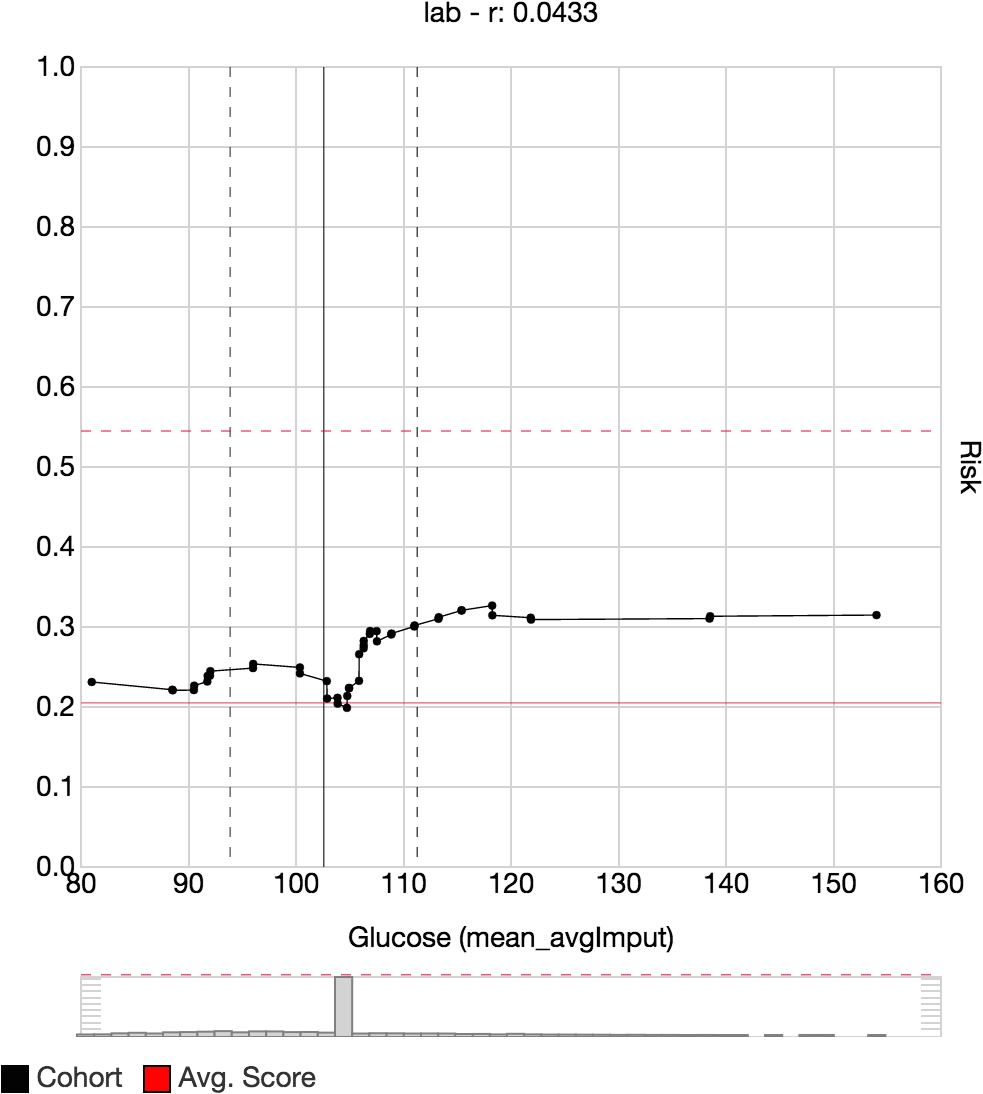
\includegraphics[width=\linewidth]{figs/prospector/debug} % 19.5
\end{minipage}\hfill
\begin{minipage}[c]{0.6\textwidth}
\caption{
Debugging model performance using partial dependence.
Instead of a direct relationship between higher Glucose lab values (x-axis) and higher risk scores (y-axis)
the model predicts a low risk for average Glucose lab values.
The histogram below the plot, showing the distribution of the values found in the input data, indicates that most patients have the average value.
% As can be seen in the distribution of the values as seen in the data set (histogram below the plot) most patients have the average value.
Since missing values are imputed using the average Glucose value the valley in the plot
can be explained by the outcome independence of this value due to the high number of missing values.
}
\label{figs:prospector_debug}
\end{minipage}
\end{figure}

% \figref{figs:prospector_debug} shows how partial dependence can be used to debug machine learning models in \textbf{Prospector}. In this example imputation of missing values created unexpected behaviour of the inspected
% classifier. Partial dependence is given by
% \[
% pdp_f(v) = \frac{1}{N} \sum_i^N pred(x_i) \;\text{with}\; x_{if} = v
% \]
% where $N$ is the number of rows in the input matrix $x$,
% $pred$ is the prediction function that takes one input row, a feature vector, and returns a prediction score,
% and $f$ is the feature used to compute the partial dependence plot.
% The formula computes the average outcome over all input rows while changing the value of feature $f$ to the
% input value $v$ for each row $x_i$. The original input data is kept fixed. This allows for observing the influence of $f$
% on the prediction scores. Unlike generalized additive models, \emph{eg.,}~\cite{Caruana:2015:IMH:2783258.2788613}, this technique is model agnostic.

% \textbf{Prospector} also supports localized inspection, so users can understand why certain data results in a specific prediction, and even lets users hypothesize new data by tweaking values and seeing how the predictive model responds.  Users can interactively tweak feature values and see how the prediction responds, as well as find the most impactful features using a novel model agnostic local feature importance metric that only depends on partial dependence.

% \begin{figure}
\centering
\begin{minipage}[c]{0.35\textwidth}
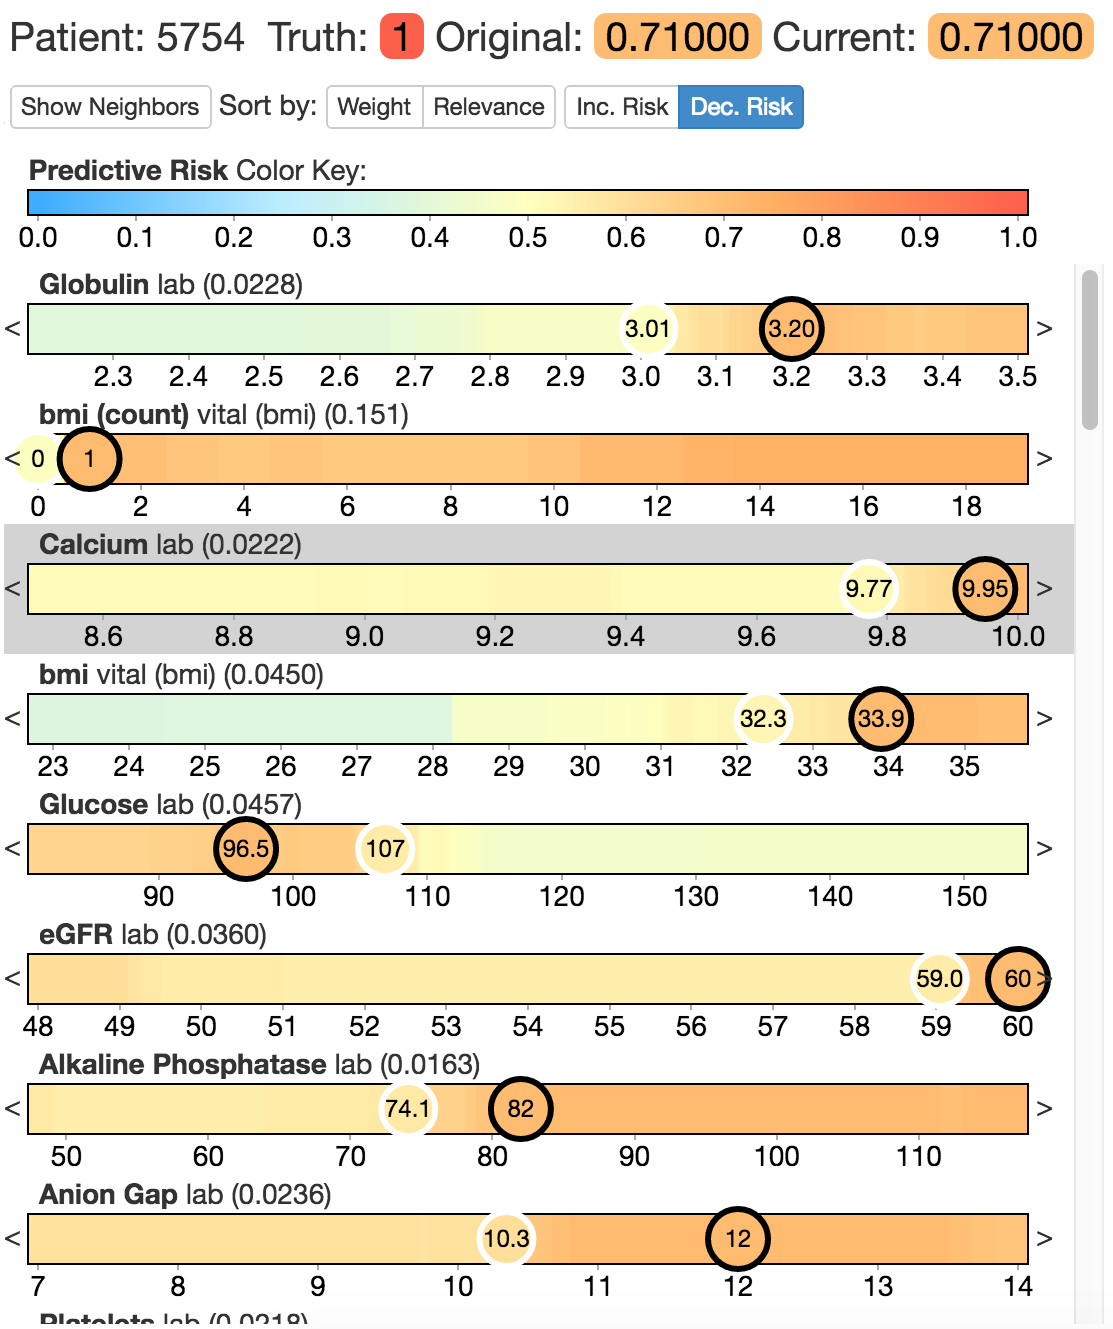
\includegraphics[width=\linewidth]{figs/prospector/dec_risk_compact} % 19.5
\end{minipage}\hfill
\begin{minipage}[c]{0.6\textwidth}
\caption{
Identifying changes to features that reduce the risk of a high risk patient.
The features are sorted by decreasing impact to make large sets of features manageable.
The background color of each feature indicates the predicted risk for this value.
Impossible values, if known, appear grayed out and the slider snaps back to the last possible value if selected.
}
\label{figs:prospector_risk}
\end{minipage}
\end{figure}

% \figref{figs:prospector_risk} shows the prediction inspection portion of the \textbf{Prospector} UI, which allows users to examine the features contributing to the prediction of a selected data point. All of the features’ partial dependence bars are shown in a scrollable list, with the data's feature values set with circular labels. Users can drag the circular label to change the value of any feature and see the prediction change in real-time.
% % Users can also select a feature and see the corresponding typical partial dependence plot of the feature. In this plot the local partial dependence of the current data point is shown as black curve and the global partial dependence of the whole population of data points is shown in gray. The partial dependence plot is also clickable and users can change the feature value here as well, changing the black vertical line that, in this plot, shows the current value.
% Users can change the sort order of the partial dependence bars by using the buttons at the top. In addition to sorting by the feature weight and relevance as determined by the predictive model if available, users can also sort according to our local feature importance and impactful changes. If impactful changes are chosen as the sort order, the suggested changes to each feature are indicated with a white circular label in the partial dependence bar.

\chapter{Explainer}
\label{chap:explainer}
% $Id: template.tex 11 2007-04-03 22:25:53Z jpeltier $
% \documentclass{vgtc}                          % final (conference style)
%\documentclass[review]{vgtc}                 % review
%\documentclass[widereview]{vgtc}             % wide-spaced review
% \documentclass[preprint]{vgtc}               % preprint -- use for arxiv
%\documentclass[electronic]{vgtc}             % electronic version

%% Uncomment one of the lines above depending on where your paper is
%% in the conference process. ``review'' and ``widereview'' are for review
%% submission, ``preprint'' is for pre-publication, and the final version
%% doesn't use a specific qualifier. Further, ``electronic'' includes
%% hyperreferences for more convenient online viewing.

%% Please use one of the ``review'' options in combination with the
%% assigned online id (see below) ONLY if your paper uses a double blind
%% review process. Some conferences, like IEEE Vis and InfoVis, have NOT
%% in the past.

%% Figures should be in CMYK or Grey scale format, otherwise, colour 
%% shifting may occur during the printing process.

%% These few lines make a distinction between latex and pdflatex calls and they
%% bring in essential packages for graphics and font handling.
%% Note that due to the \DeclareGraphicsExtensions{} call it is no longer necessary
%% to provide the the path and extension of a graphics file:
%% 
\includegraphics{diamondrule} is completely sufficient.
%%
% \ifpdf%                                % if we use pdflatex
%   \pdfoutput=1\relax                   % create PDFs from pdfLaTeX
%   \pdfcompresslevel=9                  % PDF Compression
%   \pdfoptionpdfminorversion=7          % create PDF 1.7
%   \ExecuteOptions{pdftex}
%   \usepackage{graphicx}                % allow us to embed graphics files
%   \DeclareGraphicsExtensions{.pdf,.png,.jpg,.jpeg} % for pdflatex we expect .pdf, .png, or .jpg files
% \else%                                 % else we use pure latex
%   \ExecuteOptions{dvips}
%   \usepackage{graphicx}                % allow us to embed graphics files
%   \DeclareGraphicsExtensions{.eps}     % for pure latex we expect eps files
% \fi%

%% it is recomended to use ``\autoref{sec:bla}'' instead of ``Fig.~\ref{sec:bla}''
% \graphicspath{{figs/}{pictures/}{images/}{./}} % where to search for the images

% \usepackage{microtype}                 % use micro-typography (slightly more compact, better to read)
% \PassOptionsToPackage{warn}{textcomp}  % to address font issues with \textrightarrow
% \usepackage{textcomp}                  % use better special symbols
% \usepackage{mathptmx}                  % use matching math font
% \usepackage{times}                     % we use Times as the main font
% \renewcommand*\ttdefault{txtt}         % a nicer typewriter font
% \usepackage{cite}                      % needed to automatically sort the references
% \usepackage{tabu}                      % only used for the table example
% \usepackage{booktabs}                  % only used for the table example
%% We encourage the use of mathptmx for consistent usage of times font
%% throughout the proceedings. However, if you encounter conflicts
%% with other math-related packages, you may want to disable it.

% \usepackage{amsmath}
% \usepackage{balance}  % to better equalize the last page
%\usepackage[T1]{fontenc}
% \usepackage{txfonts}
% \usepackage[pdftex]{hyperref}
% \usepackage{url}      % llt: nicely formatted URLs
% \usepackage[usenames,dvipsnames]{xcolor}
% \usepackage{color}
% \usepackage{xspace}
% \usepackage{csquotes}
% \usepackage{algorithm}
% \usepackage[noend]{algpseudocode}
% \usepackage{silence} % hangs with new template
% \WarningFilter{caption}{Unsupported document class}

% \newcommand{\comment}[2]{\textcolor{#1}{#2}}
% \newcommand{\comment}[2]{#2}

% \newcommand{\joschi}[1]{\comment{NavyBlue}{#1}}
% \newcommand{\enrico}[1]{\comment{Orange}{#1}}
% \newcommand{\aritra}[1]{\comment{Purple}{#1}}
% \newcommand{\aritranew}[1]{\comment{Red}{#1}}
% \newcommand{\yin}[1]{\comment{OliveGreen}{#1}}
% \newcommand{\jordan}[1]{\comment{Orchid}{#1}}
% \newcommand{\eg}{\emph{e.g.}\xspace}
% \newcommand{\etal}{\emph{et al.}\xspace}
% \newcommand{\ie}{\emph{i.e.}\xspace}
% \newcommand{\etc}{\emph{etc.}\xspace}
% \newcommand{\wrt}{\emph{w.r.t.}\xspace}

% \newcommand{\tabA}{Statistical Summary View\xspace}
% \newcommand{\tabB}{Explanation Explorer\xspace}
% \newcommand{\tabC}{Item Level Inspector\xspace}

% % \newcommand{\ainfo}[1]{\phantom{#1}}
% \newcommand{\ainfo}[1]{#1}

%% If you are submitting a paper to a conference for review with a double
%% blind reviewing process, please replace the value ``0'' below with your
%% OnlineID. Otherwise, you may safely leave it at ``0''.
% \onlineid{0}

%% declare the category of your paper, only shown in review mode
% \vgtccategory{Research}

%% allow for this line if you want the electronic option to work properly
% \vgtcinsertpkg

% \usepackage{caption,subcaption}

%% In preprint mode you may define your own headline.
% \preprinttext{To be published at the IEEE Conference on Visual Analytics Science and Technology (IEEE VAST 2017).}

%% Paper title.

% \title{A~Workflow~for~Visual~Diagnostics~of~Binary~Classifiers using~Instance-Level~Explanations}

%% This is how authors are specified in the conference style

%% Author and Affiliation (single author).
%%\author{Roy G. Biv\thanks{e-mail: roy.g.biv@aol.com}}
%%\affiliation{\scriptsize Allied Widgets Research}

%% Author and Affiliation (multiple authors with single affiliations).
%%\author{Roy G. Biv\thanks{e-mail: roy.g.biv@aol.com} %
%%\and Ed Grimley\thanks{e-mail:ed.grimley@aol.com} %
%%\and Martha Stewart\thanks{e-mail:martha.stewart@marthastewart.com}}
%%\affiliation{\scriptsize Martha Stewart Enterprises \\ Microsoft Research}

%% Author and Affiliation (multiple authors with multiple affiliations)
% \author{Roy G. Biv\thanks{e-mail: roy.g.biv@aol.com}\\ %
%         \scriptsize Starbucks Research %
% \and Ed Grimley\thanks{e-mail:ed.grimley@aol.com}\\ %
%      \scriptsize Grimley Widgets, Inc. %
% \and Martha Stewart\thanks{e-mail:martha.stewart@marthastewart.com}\\ %
%      \parbox{1.4in}{\scriptsize \centering Martha Stewart Enterprises \\ Microsoft Research}}


% \author{
% Josua Krause\thanks{e-mail: josua.krause@nyu.edu}\\ %
% \parbox{1.0in}{\scriptsize \centering NYU~Tandon School~of~Engineering} %
% \and Aritra Dasgupta\thanks{e-mail: aritra.dasgupta@pnnl.gov}\\ %
% \parbox{1.0in}{\scriptsize \centering Pacific~Northwest National~Laboratory} %
% \and Jordan Swartz\thanks{e-mail: jordan.swartz@nyumc.org}\\ %
% \parbox{1.0in}{\scriptsize \centering NYU School~of~Medicine} %
% \and Yindalon Aphinyanaphongs\thanks{e-mail: yin.a@nyumc.org}\\ %
% \parbox{1.0in}{\scriptsize \centering NYU School~of~Medicine} %
% \and Enrico Bertini\thanks{e-mail: enrico.bertini@nyu.edu}\\ %
% \parbox{1.0in}{\scriptsize \centering NYU~Tandon School~of~Engineering} %
% }

%% A teaser figure can be included as follows, but is not recommended since
%% the space is now taken up by a full width abstract.
%\teaser{
%  \includegraphics[width=1.5in]{sample.eps}
%  \caption{Lookit! Lookit!}
%}

%% Abstract section.
\begin{quote}\textit{
Human-in-the-loop data analysis applications necessitate greater transparency in machine learning models for experts to understand and trust their decisions. To this end,   
we propose a visual analytics workflow to help data scientists and domain experts explore, diagnose, and understand the decisions made by a binary classifier.
The approach leverages ``instance-level explanations", measures of local feature relevance that explain single instances, and uses them to build a set of visual representations that guide the users in their investigation.
The workflow is based on three main visual representations and steps:
one based on aggregate statistics to see how data distributes across correct / incorrect decisions;
one based on explanations to understand which features are used to make these decisions;
and one based on raw data, to derive insights on potential root causes for the observed patterns.
The workflow is derived from a long-term collaboration with a group of machine learning and healthcare professionals who used our method to make sense of machine learning models they developed.
The case study from this collaboration demonstrates that the proposed workflow helps experts derive useful knowledge about the model and the phenomena it describes, thus experts can generate useful hypotheses on how a model can be improved.
}\end{quote}
% The case study from this collaboration demonstrates that the proposed method helps experts derive useful knowledge about the model and the phenomena it describes and also generate useful hypotheses on how a model can be improved.

% Machine learning models are most effective when they can objectively describe and predict real-world phenomena. Effectiveness subsumes two factors: the features of the data used in the predictions are correct and useful, and the decisions made by the model are free of biases. Given large, high-dimensional datasets, modelers and users are faced with the challenge of evaluating the degree of effectiveness of a model and subsequently improve the model so that it better captures their domain knowledge. Current methods lack a systematic strategy for semantic validation of models, where a modeler or a user can identify the reasons behind a model’s decisions and validate their quality with respect to the feature space. To fill this gap, we propose an interactive workflow based on instance-level visual explanations that serves a two-fold purpose: i) makes the connections between model decisions and features explicit for subsets of instances, and ii) helps modelers and users validate and trust the decisions by exploring the explanations behind the decisions. We validate our approach by creating artificial datasets with known biases and identifying those biases with our method. We also demonstrate the efficacy of our workflow with a long-term case study about improving wait time in the emergency department of hospitals.

% Modern machine learning techniques have made it possible to accurately model almost any phenomenon.
% However, when solving problems using machine learning oftentimes gathering the correct data is the biggest challenge.
% Great care has to be taken to not introduce biases or capture data that does not have the ability to fully solve the problem.
% In order to assist modelers in improving their \textit{data} we propose an interactive workflow alongside a visual user interface utilizing item level explanations of decision made by machine learning models.
% The workflow helps to understand how the model views the data enabling a user to understand the model's and the data's shortcomings and subsequently validate and trust them.
% Furthermore, we validate our approach by creating artificial datasets with known biases and identifying those biases with our method.
% We demonstrate our workflow with a long-term case study about improving wait time in the emergency department of hospitals.

\begin{contributions}{Foo}
\item \todo{TODO}
\end{contributions}

\begin{quote}
\textit{Josua Krause, Aritra Dasgupta, Enrico Bertini}
\end{quote} % end of abstract

% \keywords{Machine Learning, Interpretation, Visual Analytics.}

%% ACM Computing Classification System (CCS). 
%% See <http://www.acm.org/class/1998/> for details.
%% The ``\CCScat'' command takes four arguments.

% \CCScatlist{ 
%   \CCScat{K.6.1}{Management of Computing and Information Systems}%
% {Project and People Management}{Life Cycle};
%   \CCScat{K.7.m}{The Computing Profession}{Miscellaneous}{Ethics}
% }

%% Copyright space is enabled by default as required by guidelines.
%% It is disabled by the 'review' option or via the following command:
% \nocopyrightspace

%%%%%%%%%%%%%%%%%%%%%%%%%%%%%%%%%%%%%%%%%%%%%%%%%%%%%%%%%%%%%%%%
%%%%%%%%%%%%%%%%%%%%%% START OF THE PAPER %%%%%%%%%%%%%%%%%%%%%%
%%%%%%%%%%%%%%%%%%%%%%%%%%%%%%%%%%%%%%%%%%%%%%%%%%%%%%%%%%%%%%%%%

% \begin{document}

\section{Introduction}

% \maketitle

% \section{Introduction} %for journal use above \firstsection{..} instead

In this paper we propose an interactive workflow and a visual user interface to help data scientists and domain experts diagnose and validate binary classifiers. The approach we suggest is based on a mix of automated and interactive methods that guide the user towards understanding what decisions a model makes, which ones are correct or incorrect, and potential strategies to improve them.

Being able to explore the decisions a model makes and identifying potential issues is crucial in application areas where experts need to get a sense of how the model works and build trust in its decisions. While common practice in much of the machine learning endeavors is to focus on model accuracy, many researchers have voiced the need for more transparency when the application domain requires it~\cite{baesens2003using, Caruana:2015:IMH:2783258.2788613, freitas2014comprehensible, lou2012intelligible, martens2007comprehensible, vellido2012making}. A recent DARPA (Defense Advanced Research Projects Agency) program called ``Explainable AI (XAI)", for example, calls for more research in this area and declares, as the main motivation for the program that ``\textit{the effectiveness of these systems is limited by the machine’s current inability to explain their decisions and actions to human users}" and that ``\textit{it is essential to understand, appropriately trust, and effectively manage an emerging generation of artificially intelligent machine partners}".

In addition to evaluating a model in terms of accuracy, we propose the idea of \textit{semantic validation}, the need for domain experts to verify that the decisions a model makes are plausible when compared against their mental models of the problem. For instance, in healthcare settings, medical doctors often want to see examples of recommendations the model provides and need to gain trust in it before they feel comfortable with deploying it in real-world settings.
Such reservations in deploying models without having an opportunity to manually verify what decisions they make are well justified as it is entirely possible for a model to achieve high accuracy and yet provide dramatically erroneous recommendations~\cite{Caruana:2015:IMH:2783258.2788613}.

Another important factor to consider is that domain experts and data scientists are often working in collaboration to solve a particular problem (or they are actually the same person covering both roles). Being able to manually inspect a model can give them an opportunity to generate useful insights on how a model can be improved. While commonly used aggregate statistics such as area under the curve (AUC) give a sense of the overall accuracy of the model, and can be used as a parameter to compare between different models, they do not provide insights on how or why a model fails to capture important phenomena accurately.

Some existing methods do provide more transparency and useful information for enabling better understanding and diagnostic purposes, but they tend to be limited and specific to a particular kind of model. For example, \textit{logistic regression} and \textit{decisions trees} are commonly regarded as more interpretable models thanks to their ability to provide information on feature weights and / or specific decisions the model makes (decision trees)~\cite{freitas2014comprehensible}. These solutions are however limited by a number of factors. Since they are specific to the selected method, they are hard to generalize and cannot be applied transparently to other types of models. Furthermore, they only provide a limited picture of what decisions the model makes. Feature weights provide a highly coarse summary of how relevant features are \textit{globally}, but they do not provide information on how the model makes decisions \textit{locally}, for a selected set of instances. Even more transparent methods, like decision trees, tend to grow very large and are not easy to parse visually, especially for data sets with a high number of dimensions / features.

\input{explainer/workflow}

To address these issues we propose a workflow, aimed at machine learning experts and data scientists, based on \textit{instance-level explanations}, computational methods to derive a description of how a model makes decisions on single data items, without having access to the internal logic of the model (\ie, using the model as a \textit{black box}). These explanations are then aggregated and used as input to a visualization system that enables the browsing of model decisions and assessment of their quality.

The work we describe in the paper stems from a one year collaboration with a group of domain and machine learning experts~from the \textit{NYU Langone Medical Center}.
%~({two of them are co-authors of this paper})
In our collaboration, we worked together to make sense of models built to understand how patients are handled in the hospital and to figure out whether important outcomes of interest can be predicted correctly. This resulted in the development of an interactive model diagnostic workflow using visual explanations of model behavior that is the main contribution of this work.
% main outcome of this interaction is the workflow and interfaces we describe in the paper
% \aritra{I feel this paragraph about section organizations is not needed.}
The rest of the paper is organized as follows. We present related work in the next section. We provide an overview of model diagnostics goals and of the proposed workflow in Section~\ref{sec:model-diagnostics}. We then describe in detail the instance-level explanation algorithm we use in Section~\ref{sec:algo} and the interfaces we built in Section~\ref{sec:ui}. Section~\ref{sec:case_study} reports on a use case we built to show how the workflow can help perform useful and actionable model diagnostics. Section~\ref{sec:discussion} discusses the results and provides a number of reflections and lessons we have learned from this collaborative exercise.

%In our work, we use a method developed by Marteens et al.~\cite{}, which works on binary classification with sparse high-dimensional data set and creates explanations in form of the set of features the model uses to make a decision on a single instance.



% ---
% when using predictive modeling as part of their analysis workflow, are frequently confronted with questions as: ``Do the model predictions make sense?", ``Can I trust this model?" To answer these questions, merely optimizing the model performance for achieving the best match between predicted and actual outcomes is not sufficient. Statistical performance measures can indicate correctness, but they do not ensure that the model is actually plausible and can be trusted.

% While a very large proportion of the efforts in predictive modeling is on achieving accurate \textit{predictions}, little has been done to systematically assure that a model is able to provide plausible \textit{explanations} of the intricate set of relationships between features, their values, and the outcome. To fill this gap, we propose a diagnostic workflow that can enable both data scientists and non-machine learning domain experts in \textit{semantic validation} of binary classifiers by observing input-output relationships of models through the lens of visual explanations.

% We derive this workflow through a long-standing collaboration with doctors and healthcare experts. In healthcare settings it is crucial to derive insights on \textit{why} and \textit{how} a model relates a set of patient descriptors (patient history) to a given medical outcome of interest (disease onset). In this scenario, global explanations of model behavior are not sufficient: experts often need to focus on subsets of patients or a single patient, find features related to the predicted label, verify if they are meaningful, and accordingly get insight into both global and local predictions of the classifier. To address this, at the core of our workflow are instance-level visual explanations: explanations that are based on measures of local feature relevance for single instances in the data. These are communicated through visual representations that help guide the experts in diagnosing why and how a classifier makes its decisions.

% In our approach, we treat a classifier as a black-box. This has two advantages. First, the approach can be generalized for any existing classification model. Second, without having to access its internal structure, data scientists and domain experts alike can observe the input / output behavior of a model and diagnose model decisions for developing trust in them.

% In the rest of the paper we first investigate related work and describe the motivation and design decisions for the diagnostic workflow. Second, we focus on the description of the visual interface by mapping the domain experts' tasks to the different visual representations and interactions. Next, we describe two use cases derived from our collaboration that validate the efficacy of our workflow. We also reflect on the generalizable lessons learnt about how visual explanations can be used to inspire trust in domain experts about the semantic validity of model predictions.







% Requires semantic validation, going beyond statistical measures of model performance. drawbacks: lack of generalizability, most applications for model tuning.

% We derive a workflow, healthcare, model diagnsotics. data scientists: features that are necessary, domain experts, incorporate their domain knowledge


% \begin{itemize}
%     \item \joschi{TODO -- commented old introduction which doesn't focus on explanations for debugging though}
% \end{itemize}
% \joschi{rewrite}
% In this paper we use visual analytics to discover and explore explanations of decisions made by a binary classifier. \joschi{TODO: too vague}

% Many real-world scenarios require analysts to understand how a set of many independent features and a target of interest relate to each other; that is, which combinations of features and values lead to a given outcome. For example, this includes: how words used in product reviews relate to the number of stars assigned by reviewers or how physiological measures and medications affect patient admission in a hospital.

% Predictive modeling using classification techniques is a very common approach to solve those kind of problems as classification methods are meant to build models that capture associations between values and a target. Experts usually optimize those models for achieving the best match of predicted and actual outcomes. While this is necessary for predictive modeling to work correctly it does not ensure that the model is actually plausible and to be trusted.

% \joschi{example of a situation -- pneumonia/astma example of \url{http://people.dbmi.columbia.edu/noemie/papers/15kdd.pdf}}

% For instance, in healthcare settings it is crucial to derive insights on \textit{why} and \textit{how} a model relates a set of patient descriptors (patient history) to a given medical outcome of interest (disease onset) in order to be actually useful in practice and trusted by doctors. Even if the prediction of the model is always correct on the test data set; without confirming the correctness of the decision \textit{making} process the correctness of the model cannot be guaranteed in general.

% While a very large proportion of the efforts in predictive modeling is on achieving accurate \textit{predictions}, little has been done to systematically assure that a model is able to provide plausible \textit{explanations} of the intricate set of relationships between features, their values, and the outcome.

% \joschi{what are you actually proposing here?}
% A common approach of giving insights into the decision making
% process of a machine learning model is to assign importance
% to features in the data set.
% This is usually done globally without regard for individual nuances (\joschi{TODO: cite some papers maybe?}).
% Thus, this does not provide insights into actual decisions
% being made but rather how influential certain features
% are in general.

% A more sophisticated approach that is gaining more popularity
% recently \cite{prospector,Martens:2014:EDD:2600518.2600523,DBLP:journals/corr/RibeiroSG16} is to locally assign feature importance to individual items.
% This is achieved by generating hypothetical inputs to the machine learning model to examine how an observed data point needs to be changed in order to \textit{change} the predicted outcome.
% This gives insight into which features are responsible for the original prediction of the observed data point.
% The set of locally important features is thus called the ``explanation" of a data point.

% This approach generates individual explanations for every observed
% item in the data set.
% Using aggregation and visual analytics helps coping with this vast amount of additional meta data enabling domain experts to analyze the correctness of the decision making process on a population level rather than on a case-by-case basis.

% \joschi{TODO: give teaser of the VA interface -- HOW still missing}

% Our contributions are concretely:
% \begin{itemize}
%     \item Tasks needed to check plausibility of and gain trust in decisions made by a machine learning model.
%     \item A rich visual analytics application aimed at solving those tasks.
% \end{itemize}

% \joschi{TODO: paper structure}

\section{Related Work}
% \begin{itemize}
%     \item \joschi{model tracker looking at prediction score distribution and single items}
%     \item \joschi{specialized models aka GAM}
%     \item \joschi{TODO more and categorize papers}
% \end{itemize}

In the following, we discuss model explanations and visual analytics techniques used for interacting with classification models.

\subsection{Model Explanations: \textit{Why} and \textit{How}}

Explanations of behavior of autonomous systems~\cite{Lim:2009:ADI:1620545.1620576} or computational models~\cite{dasgupta2017familiarity} can lead to a high degree of human-machine trust. In machine learning, model explanations are beginning to be used in human-in-the-loop data analysis applications for communicating information about model behavior and predictions. While there are some studies~\cite{harmful} that show that explanations can lead to over-reliance on the system, generally it has been posited that model explanations lead to a high degree of human interpretability and trust~\cite{lipton2016mythos}. Similar to the latter, our goal in this work was to develop a visual analytic workflow for model explanations and to work closely with data scientists and domain experts to understand how that could lead them to understand and trust model behavior.

In the literature, we find two contrasting purposes behind generating model explanations. The first approach is embedded within the interactive machine learning pipeline and helps end users in refining a model's predictions by interacting with the model structure. This helps users to build a mental model about the model reasoning process~\cite{Kulesza:2015:PED:2678025.2701399}. Through the EluciDebug approach, Kulesza \etal lay out a set of principles for the process of explanatory debugging using a Na\"ive Bayes classifier model.
Although the principles are generally applicable, the explanation technique is specifically applicable only to a particular model.
Furthermore, additive models enable intuitive explanations through feature contributions that allow both to visualize the decision making process for single instances \cite{Poulin:2006:VEE:1597122.1597143} and feature contributions on a population level \cite{Caruana:2015:IMH:2783258.2788613}.
However, this solution requires the use of an additive model and as such it is not generally applicable.

To overcome this limitation, a second approach for explanation generation is to treat the machine learning model as a black box, bypassing the model structure, while communicating the input-output relationships and their relevance to a model's decisions to an analyst, \eg, inferring rules from a neural network~\cite{Craven98usingneural}, or generating explanations~\cite{DBLP:journals/corr/RibeiroSG16,prospector}. We adopt this black-box approach in our workflow for benefiting domain experts, who are not trained in machine learning, and also for providing data scientists with a model-agnostic and generalizable diagnostic interface for inspecting model quality. In previous work, local explanations have been used to diagnose how models make decisions for single instances of a data set~\cite{infuse,prospector,DBLP:journals/corr/RibeiroSG16}.
In contrast, we provide an interactive workflow where users can explore aggregated representations of explanations and better understand the context of model decisions by iterating across explanation-level and instance-level visual summaries of prediction quality.  

% local explanations for deriving more holistic insights about the validity of model decisions. 





% \subsection{Analyzing Model Predictions}



% What questions data scientists or domain experts are interested in while analyzing the quality of model predictions?

\vspace*{-1em}
\subsection{Human-in-the-Loop Inspection of Classifiers}%Classification Models}
\vspace*{-0.5em}
Researchers have recently demonstrated how human interventions can help in greater accuracy in construction of classifiers, when compared with a purely automated approach~\cite{tam2017analysis}. In this work, Tam \etal used information theory to show how soft knowledge of model developers can be encoded in decision trees, and they advocate a tighter integration between human and machine-centric processes for model development. The goals for integrating visual analytic techniques and classification methods fall broadly into three categories, as proposed by Liu \etal~\cite{liu2017towards}: i) model understanding, ii) model diagnosis, and iii) model refinement. Our proposed diagnostic workflow~(Figure~\ref{figs:workflow}) encompasses the goals of understanding model behavior and diagnosing the model decision space for enabling data scientists and domain experts to generate insights about potential inadequacies in the data and in the model quality. The refinement step is an obvious action as a result of these insights, but is outside the scope of our work.

Analyzing summary statistics of model performance through the lens of visualization techniques is the most common approach for finding matches and mismatches between model predictions and ground truth data. To this end, ModelTracker~\cite{amershi15} provides a unified interface for error detection and debugging for binary classifiers showing item-wise distributions of prediction scores. Bilal \etal propose the confusion wheel visualization~\cite{alsallakh2014visual} and other linked views to show probabilities of items belonging to different classes for multi-class classifiers.  Squares~\cite{ren2017squares} provides a single, unified visualization of performance metrics and easy accessibility to the data for debugging multi-class classifiers. For enhancing the interpretability of classifier predictions, Cortez and Embrechts~\cite{cortez2011opening} use a sensitivity analysis approach for letting users understand the effects of variation of input values on model outputs. While these methods are able to diagnose performance issues 
at the level of a single item~\cite{alsallakh2014visual,amershi15,ren2017squares} or single features~~\cite{cortez2011opening}, they lack a holistic summary of the entire decision space that exposes associations among subsets of items and features, and communicates the reasons behind the model decisions. Through an explanation-based approach, we can let analysts explore these associations for a large, high-dimensional data set, drill-down to individual items, and diagnose potential problems with respect to both global and local decisions. This leads to actionable insights about the limits to which model quality can be improved, and ultimately, hints about how to improve the data.

% %  \joschi{
% As preliminary work we published previous iterations that helped to shape the proposed workflow here.
% In \cite{class_signatures} we investigated alternative methods of grouping the data.
% % set by relying solely on prediction scores of the model.
% However, we realized that those methods mostly reflect the intrinsic structures of the data set instead of the decision making process of the model.
% As such, detected relations stay superficial as those relations cannot be sufficiently complex to match those of a machine learning model.
% In \cite{rivelo} we investigated model exploration capabilities of explanations by focusing on common features in explanations. This approach shows which features were used for predicting in general, which is at odds with mainly focusing on strongly correct or problematic behavior.
% % }

% Probabilistic Classifiers.

% While a class of visual analytic techniques that help in feature selection~\cite{infuse,choo2010ivisclassifier} and feature engineering~\cite{brooks2015featureinsight,heimerl2012featureforge}, they work with the assumption that high quality data and useful features are already available to the model. In contrast the explanations we provide help analysts to use their domain knowledge and detect if the features used by the model are relevant, and how different combinations can be used to improve the prediction scores. 


% \begin{itemize}
%     \item Common method for analyzing quality of model predictions is by looking into summary statistics. Tools exist for visualizing model performance interactively (ModelTracker\cite{amershi15}, Squares\cite{ren2017squares}) Sensitivity Analysis.\cite{cortez2011opening}
%     \item A concrete example why performance measures are necessary but not sufficient. Do we have one example paper we can cite?
%     \item We use explanations as a richer way to expose the associations among items, features and labels, and diagnose why a model made a particular decision.
% \end{itemize}

% role of human in the loop:\cite{tam2017analysis}

% Feature Engineering: 

% \cite{infuse} Infuse

% \cite{brooks2015featureinsight} FeatureInsight

% \cite{heimerl2012featureforge} FeatureForge

% \cite{alsallakh2014visual} Probabilistic Classification Models.

% \cite{choo2010ivisclassifier} IvisClassifier

% Semantic Quality: (degree to which the predictions reflect reality and features used in those predictions make sense for a domain expert)
% \cite{rheingans2000visualizing}


\section{Model Diagnostics}
\label{sec:model-diagnostics}

We use the term \textit{Model Diagnostics} to indicate the steps necessary for a domain expert or a model developer to semantically validate the decisions made by a model using their domain knowledge. In this section we outline the different goals for a user when using a model diagnostic interface and provide an overview of the implementation of the resulting workflow~(Figure~\ref{figs:workflow}). 
The workflow was derived through a long term collaboration among visual analytic researchers and model developers and domain experts in the medical field, specifically in the application scenario of hospital visits. The over-arching goal in this scenario is to use predictive modeling for reducing patient wait time and optimizing the hospital resources needed for admitted patients.

% The main purpose of the workflow we propose is to support the experts in answering the following key questions for model understanding and diagnostics.

\subsection{User Goals}

In the course of our interactions with domain and machine learning experts and analyzing a variety of model building problems, we realized that the model diagnostics problem can be decomposed into the following main goals; which we express as a set of questions as shown in Figure~\ref{figs:workflow}.  

% \aritra{There is a lot if literature on model performance analysis. We should explain what we mean by diagnostics and why it goes beyond performance analysis.}

\textit{G1: What is the overall accuracy of the model?} In this step, experts need to get an overview of the distribution of prediction scores across the data items, derive an understanding about the uncertainty associated with predictions of certain items, and generally where the predictions are correct or incorrect.

%A simple manual inspection of prediction scores for large, high-dimensional data sets is often inefficient as significant number of iterations are required between switching between analysis of predictions scores and the associated sets of features and items.

\textit{G2: What are the main decisions the model makes?} A trained classifier creates a decision space that maps a (potentially high-dimensional) input space into the output space defined by the two labels \textit{true} and \textit{false}. Understanding what these decisions are and how frequently they are made is a crucial piece of knowledge domain experts want to draw from the classifier. For instance, in the healthcare scenario we explore in this paper it is crucial for domain experts to know that the vast majority of decisions the classifier makes are based on a small set of drugs (features). They also want to ensure that different sets of drugs are used by the classifier to make decisions about different sets of patients (\eg, a group of patients is characterized by \emph{Ondansetron} and \emph{Sodium Chloride}, whereas another is characterized by antibiotic drugs).

\textit{G3: How accurate are the decisions the model makes?} Together with knowing what decisions the model makes, it is crucial to also know how accurate these decisions are. Using the same example as above, it is not sufficient to know that the model classifies a group of patients according to the drugs they received, but also how often this decisions are correct or incorrect.

\textit{G4: How can one change the data or the model to improve its decisions}? Understanding decisions and assessing their accuracy is relatively useful, but the ultimate goal for a model developer is to actually gain \textit{actionable} insights on how the model can be \textit{improved}. Some of the insights experts want to derive include: whether the model parameters should be tuned or a better set of features should be derived.

% \aritra{added some text to refer to the figure}
In this work we do not provide specific support for the actual parameter tuning or data processing steps necessary to improve the model.
The black-box nature of our approach is illustrated in Figure~\ref{figs:workflow}, which shows that the model diagnostic workflow is an extension of (and not a part of) the existing model building workflows that data scientists follow as part of their routine. Modelers have specific ways and tools to perform these steps and intervening on their established practices is out of the scope of this work. Rather, in this work we focus on providing support for the diagnostic part experts may want to execute at the end of each modeling round and which is currently not well supported by existing tools and practices.
% Our workflow takes a trained model as an input.
The diagnostic insights produced by our workflow provides hints about whether the input data or the model structure needs to be changed for improving the prediction quality.

\subsection{Workflow}
\label{sec:workflow}

% \aritra{edited to remove redundancy and make terms used more clear.}

The workflow we propose results from two pre-processing operations: \textit{explanation generation} and \textit{visual mapping}.

\textit{Explanation generation} takes as an input a data set and a trained binary classifier and creates for each instance in the data set an \textit{explanation}. An explanation is a description of the logic (or rule) the classifier uses to assign a given label to the instance. For this purpose, we leverage a method developed by Martens and Provost~\cite{martens2007comprehensible}, which computes, for a given instance which features need to be ``removed" in order to change the classification outcome. For instance, in a text classification problem, an explanation for a document consists of the words that need to be removed in order to change the label originally assigned by the classifier. In Section~\ref{sec:algo} we describe in more detail how the explanation method works.

\textit{Visual mapping} takes as an input the data set and the set of explanations, and builds a set of interactive visualizations~(Figure~\ref{figs:workflow}) that support the user goals we outlined above. The interactive workflow revolves around three main linked interfaces; each one supporting the analysis of model decisions at different levels of granularity and addressing the user goals. 

%\aritra{Too much detail and forward referencing in the text below. We should not expect people to refer to figures that are 4-5 pages later. I also think it is too early to describe the visualizations/interface. We are also calling it "interface" here and later terming them as "panels".}

% \begin{enumerate}
\par \noindent \textbf{Outcome-level.} The first step focuses on overall accuracy of the model, using a representation similar to a confusion matrix. The main goal of this step is to get a sense of how data distributes across the prediction score computed by the classifier (typically a score between $[0, 1]$), and the four possible outcomes: true or false positive and true or false negative. By visualizing how data distributes across the four possible outcomes the user can gain a sense of how accurate the model is~(\textbf{G1}) and whether errors cluster around particular sets of scores.
    
    %Figure~\ref{figs:overview}, shows an examples of how this information is visualized. The x-axis represents the prediction score computed by the classifier, an the bars show how data distributes across the four possible outcomes: false positive (orange hatchet bars), true positive (orange bars), false negative (blue hatchet bars), and true negative (blue bars) instances.
    
\par \noindent \textbf{Feature-level.} The second step uses the computed explanations to generate an overview of decisions made by the classifier and their accuracy. Each explanation is described by the set of features it uses to explain an instance and, as such, it provides a description of how the model makes its decisions. In this step, we group together all the explanations (and thus the instances) that contain the same set of features, compute accuracy statistics on top of them, and use these groups as a visual interactive summary of the decisions the model makes. By visualizing the explanations and their accuracy the user can get a sense of what are the major decisions the model makes and how accurate they are~(\textbf{G2, G3}).
    
    %For each explanation we also compute the proportion of false / true negative / positive outcomes and visualize them as shown in Figure~\ref{figs:expl_main}. Each row represent one explanation. The labels represent the set of features contained in the explanation. And the stacked bars show how many instances are covered by the explanation and how they distribute across the four possible outcomes.
    
\par \noindent \textbf{Instance-level.} The third step focuses on the analysis of a single user-selected explanation and the instances it explains. Once an interesting explanation has been found in the previous step, it is often useful and necessary to drill-down to the individual instances to observe how the data items contained in an explanation distributes in the original data space. Being able to observe their actual data values and the decisions the model enables experts in formulating hypotheses about why the classifier fails to make correct decisions with some instances. In other words, when it is possible to visually compare the data values of instances that have the same explanation but different outcomes, users can draw inferences on the root cause of the diverging outcomes. Therefore, by visualizing single instances the user can reason on how the model makes decisions and derive potentially useful hypotheses about how they can be improved~(\textbf{G4}). 
    
    %based on a matrix layout (Figure~\ref{figs:inspect}), visualizes the set of instances contained in a user-selected explanation. Each column represents one feature in the data set and each row represents one instance. While the previous feature-level step helps gaining an overview of what decisions the model makes overall, and what features it uses for these decisions, the instance-level step helps derive more specific hypotheses about how and why a model makes its decisions on single instances.
% \end{enumerate}

These three steps are linked in a sequence by user-driven filtering mechanisms. The user can select specific sets of values at the outcome-level and visualize them at the features-level. While observing the main set of decisions at the feature-level, she or he can select specific explanations and inspect individual instances in the instance-level interface.

% These three steps support the questions we have outlined above. By visualizing how data distributes across the four possible outcomes, the user can gain a sense of how accurate the model is overall and whether the errors cluster around particular sets values. By visualizing the explanations and their accuracy the user can get a sense of what are the major decisions the model makes and how accurate they are. By visualizing single instances the user can reason on how the model makes decisions and derive potentially useful hypotheses and how it can be improved (we will provide specific examples in the case study in Section~\ref{sec:case_study}).

It is important to stress the key role explanations play in the workflow. By computing the explanations and computing statistics on top of them we can effectively provide a description of the main set of decisions the model makes \textit{without} having access to the internal logic of the model. The relevant aspect of explanations is that they compute a compact description of which features the model uses to make \textit{local} decisions for a \textit{subset} of instances. 
For example, in the medical data analysis explored in this work, where each patient is described by the medications he or she received (features) and the classifier predicts whether the patient will be admitted or not, an explanation can identify a group of patients characterized by a small set of medications; that is, the medications the classifier uses to make its prediction.






%We developed a model diagnostics workflow a six-month long collaboration among visual analytic researchers, machine learning modelers, and healthcare researchers and doctors ~(henceforth referred to as \textit{experts}). The collaboration involved face-to-face discussions about the common problems in their analysis pipeline. Through these interactions we developed a shared understanding of the current practices in predictive modeling of medical data and the shortcomings of the existing solutions, and derived a set of analytical goals and tasks that fit in a unified workflow and can be realized using a visual analytic interface. 


%\subsection{Challenges}
%
%\begin{itemize}
%\item Lack of flexibility
%\item greater transparency
%\item efficiency- model-specific vs model-agnostic
%\end{itemize}





%\subsection{Model Diagnostic Goals and Tasks}



%In the course of our discussions with experts, we distilled a set of high-level diagnostic goals and tasks that they intended to perform using model explanations as a core part of their workflow. In the following, we discuss the workflow with respect to the three key steps, and their associated tasks and intended outcomes as illustrated in Figure~\ref{figs:workflow}.


% \par \noindent \textbf{G1: What is the model doing?}: In this step, experts need to get an overview of the distribution of prediction scores across the data items, derive an understanding about the uncertainty associated with predictions of certain items, and generally where the predictions are correct or incorrect. A simple manual inspection of prediction scores for large, high-dimensional data sets is often inefficient as significant number of iterations are required between switching between analysis of predictions scores and the associated sets of features and items.

% The analytical tasks to address those goal are the following: 

% \par \noindent \textbf{T1.} Identify the common predictions based on the prediction scores and thresholds.
% \par \noindent \textbf{T2.} Detect any overfitting of the data by looking into performance measures. 
% \par \noindent \textbf{T3.} Get a general sense about which items are easy or difficult to predict for the classifier.

% \noindent The intended outcomes of these tasks are two-fold: i) experts may decide to use a different model that gives better performance, and ii) using statistical performance measures of models as a starting point, experts can decide to focus on items of interest by using domain knowledge of experts. 


% \par \noindent \textbf{G2: How is the model making  predictions about specific items?}: Experts often need to diagnose the causes about predictions of items of interest by probing the high-dimensional feature space and bypassing the inner workings of the model. An item-level analysis of single prediction score and a single feature vector is too granular, and it does not offer insight into groupings that might exist both itemwise and with respect to subsets of features. Clustering items in the original data space is also ineffective and potentially misleading as the data-space distances among items may not correspond with distances with respect to the model manifold, resulting in completely different outcomes for neighbors in the original space.  

% The analytical tasks to address this goal are the following: 

% \par \noindent \textbf{T4.} Use explanations as a means to group items and find groups of items with similar explanations.
% \par \noindent \textbf{T5.} Detect the most common explanations and use domain knowledge to verify if they are meaningful. 
% \par \noindent \textbf{T6.} Browse associations among features, items, and labels and inspect if the decisions lead to expected and unexpected insights.

% \noindent The intended outcome of these tasks is for experts to make associations among items, featurs, and predictive labels, to develop trust in the model's decisions by observing if relevant features are used in the predictions, and if the different groupings make sense.

% \par \noindent \textbf{G3: Why are local and global predictions different?}: Once experts have developed a general understanding of the features used in the model's decisions, they like conduct more fine-grained analysis of subsets of items and find the most discriminating features for a given subset. This can leading to finding problems with the data itself: an exact same data point having different ground truths. This implies that model diagnostics can also be used to correct errors in the data and subsequently improve the features used in the data for any given model.

% The analytical tasks to address this goal are the following: 

% \par \noindent \textbf{T7.} Identify the discriminating features for subsets of items.
% \par \noindent \textbf{T8.} Find means for correcting any model errors and make the model use alternative sets of features. 

% \noindent The intended outcome for this step is for domai experts to understand how improvements can be made to the data and feature choices for the model.

% \smallskip

%These set of diagnostic tasks were used for developing an explanatory visual analytic interface. In the following sections, we first describe our explanation algorithm~(Section 4), followed by a description of the design of the visual interface~(Section 5), and a presentation of two case studies~(Section 6) and lessons learnt from them~(Section 7).

%\subsection{Data and Model Characterization}

% The workflow we propose accepts as an input a $n$-dimensional table $D=\{f_1, \dots, f_n, T\}$, where each $f_i$ represents one \textit{feature} describing a characteristic of the objects described by the data (e.g., patients described by the medications they received) and $T$ represents the \textit{target}, that is, the outcome associated to this object (e.g., whether a patient is admitted in the hospital or not).

% In this work we focus exclusively on datasets in which both the features and the target are binary, that is, where $f_i \in \{0, 1\}$ and $T \in \{0, 1\}$. Such simplification makes the problem easier to manage while preserving sufficient relevance. Datasets with such a structure are indeed very common in predictive analytics and describe a large variety of real-world cases. In addition, many datasets that do not emit such a structure can often be transformed into binary datasets with a binary outcome through feature transformation operations. In the rest of the paper we thus assume to work exclusively with such type of data.

% The specific problem that is addressed here is for experts to understand and diagnose the predictions of a binary classifier.
% While a very large proportion of the efforts in predictive modeling is on achieving accurate \textit{predictions}, these kinds of scenarios have less to do with prediction itself and much more with whether a model is able to provide plausible \textit{explanations} of the intricate set of relationships between features, their values, and the outcome.

%The problem of model \textit{transparency} and \textit{interpretation} is important and very well recognized in machine learning, where model transparency is largely believed to be at odds with its performance; that is, models that features high predictive performance have low transparency and vice-versa~\cite{breiman2001}.



% ====> MOVE THESE TO RELATED WORK AND/OR INTRO ??? <=====

% Two main approaches are available in machine learning to allow an expert to inspect and better interpret a model. The first approach consists of training models that are \textit{intrinsically transparent}; that is, models whose structure is amenable to human interpretation. In this class of methods reside \textit{decision trees}, which produce a hierarchy of binary decisions connecting feature values to outcomes, and \textit{classifications rules}, which achieve the same goal by producing lists of logical rules (with feature values as antecedents and outcomes as consequent). All models based on linear regression, notably the popular \textit{logistic regression} and \textit{generalized additive models (GAMs)} are also somewhat amenable to human interpretations thanks to the weights they produce which communicate, for each feature, the strength and sign of its association with the outcome (\eg, positive and large weights imply a positive strong association between the feature and the outcome).

% The second approach consists of using a trained model as a black-box and deriving explanations by looking exclusively at input-output relationships obtained by probing the model. In this class of methods resides partial dependence and sensitivity analysis which both rely on strategically creating new data points to observe the reaction of the underlying model.
% %In theory, albeit not feasible in practice, all possible data points could be created to get a wholly understanding of the model.
% The main limitation of those methods is the issue of representing and exploring the results forcing the interaction to be mostly one dimensional.

% %\enrico{shall we give a name to these two approaches? Maybe white-box and black-box?}

% When we look at all these methods we can identify a number of important limitations. The first approach has \textbf{limited flexibility}. It works only with a narrow set of models and, as such, does not provide a solution for all those cases where a different method needs to be used. They also provide a very specific kind of explanatory structure (e.g., hierarchies and rules) thus preventing the use of more generic solutions. The second approach has \textbf{limited explanatory power}, mainly because all approaches limit their analysis to the relationship between a \textit{single feature} and the outcome; thus not being able to generate more expressive associations that involve \textit{multiple features}\footnote{multiple features as in arbitrary many features}
% and the outcome.

% In our approach, we consider the classifier as a black box and derive \textbf{explanations} by looking exclusively at input-output relationships obtained by probing the model. While methods like partial dependence and sensitivity analysis, which rely on strategically creating new data points to observe the reaction of the underlying model can be used for such purposes, the main limitation of those methods is the issue of representing and exploring the results forcing the interaction to be mostly one dimensional. The main goal of the workflow is to produce ``visual signatures" generated by model explanations that are able to describe existing and interesting associations between the features $f_i$ in a high-dimensional space and the target $T$.

%\begin{itemize}
%    \item \joschi{introduce healthcare application}
%    \item \joschi{doctors want to understand and trust and improve the model}
%    \item \joschi{pair of domain expert and ML modeler}
%    \item \joschi{developed user interface over months with constant back and forth}
%    \item \joschi{improving the data since model reached capacity}
%    \item \joschi{tasks:}
%    \item \joschi{prediction strength of items (using prediction score as indicator)}
%    \item \joschi{which items are easy/hard to predict}
%    \item \joschi{what are common features/predictions?}
%    \item \joschi{where is the model correct/incorrect?}
%    \item \joschi{why is that?}
%    \item \joschi{is it possible to improve those errors and if yes how?}
%    \item \joschi{problem:}
%    \item \joschi{item level analysis (ie. single prediction score, single vector) too granular}
%    \item \joschi{clustering items does not work since (original space) close data items are not necessarily close in the ML model manifold (neighbors in the original space might have completely differently strong outcomes)}
%    \item \joschi{using explanations as filter for which features actually contributed to a prediction}
%    \item \joschi{we can analyze data items with the same explanation as groups / subsets of the data}
%    \item \joschi{we propose workflow that includes explanation subsets}
%    \item \joschi{1. improving the model / experimenting with different ML techniques}
%    \item \joschi{using common model statistics to compare models: accuracy, ROC, AUC, confusion matrix, prediction score distribution}
%    \item \joschi{2. looking at explanation groupings}
%    \item \joschi{are there few general (short) explanations or many very specific (long) explanations? $\rightarrow$ overfitting (also compare train AUC to test AUC)?}
%    \item \joschi{what are the most common explanations? are they positive / negative / correct / incorrect?}
%    \item \joschi{which explanation subgroups are significant wrt. to the overall data set (odds ratio)?}
%    \item \joschi{domain experts input on sanity of explanations/predictions -- do the groupings make sense with the given prediction?}
%    \item \joschi{what is the correct / incorrect ratio of a given explanation? 100\% incorrect easy to fix just flip label but 50\% incorrect hard to fix since flipping would just make other half incorrect. are there features beside explanation that can help discriminating those cases?}
%    \item \joschi{checklist: high / low accuracy; 50\% accuracy; high / low significant odds ratio; large insignificant odds ratios}
%    \item \joschi{3. looking at items of explanation subsets}
%    \item \joschi{what are the most discriminating features for the given subset?}
%    \item \joschi{is it possible to use them to correct the mistakes?}
%    \item \joschi{would this make sense from a domain experts perspective?}
%    \item \joschi{sometimes we run into the exact same data point with different ground truths -- a domain expert is needed to determine how we can improve the data (!!! not the model !!!) to fix those problems}
%\end{itemize}

\section{Explanation Method}
\label{sec:algo}
% As preliminary work we published previous iterations that helped to shape the proposed workflow here.
% In \cite{class_signatures} we investigated alternative methods of grouping the data.
% % set by relying solely on prediction scores of the model.
% However, we realized that those methods mostly reflect the intrinsic structures of the data set instead of the decision making process of the model.
% As such, detected relations stay superficial as those relations cannot be sufficiently complex to match those of a machine learning model.
% In \cite{rivelo} we investigated model exploration capabilities of explanations by focusing on common features in explanations. This approach shows which features were used for predicting in general, which is at odds with mainly focusing on strongly correct or problematic behavior.


% The goal of explanations is to group data items from the perspective of the machine learning model being analyzed.
Using explanations, we intend to group data items from the perspective of the machine learning model being analyzed.
In order to do so without relying on a particular model, that is, treating the model as black box, we can estimate which features were involved in its decision making process.
In our initial approach, we had explored alternative methods for grouping the data by looking only at prediction scores of the model~\cite{class_signatures}. However, we realized that those methods mostly reflect the intrinsic structures of the data set instead of the decision making process of the model. Therefore, in this work we build explanations by finding the minimal amount of change necessary to change the prediction of the analyzed model, specifically, a binary classifier. Also, contrary to our previous approach of using explanations to detect only the commonly used features by a model~\cite{rivelo}, here we focus on explanations as a way for experts to diagnose correct or problematic model behavior and address the goals \emph{G1, G2, and G3}, that were outlined in Section~\ref{sec:model-diagnostics}.


% For binary classifiers this is commonly done by finding the minimal amount of change necessary to change the prediction of the analyzed classifier.
Explanations are created using a trained model by creating synthetic input values derived from observed data items revealing this input-output relationship.
The set of changes to the values that swayed the outcome of the prediction is then called explanation $e$ for the given original data item:
%
\[
\min_{e} \, L(v - e) \neq L(v)
\]
%
where $L$ is the label function with ``positive" or ``negative" as result and $v$ is the data item to be explained.
In order to compute $e$, the prediction function $P$ of the classifier is used with a threshold $t$:
%
\[
L(v) = P(v) > t
\]
%
The output of $P$, the prediction score, is a number between 0 and 1 indicating the confidence of a classifier in the predicted outcome.
The threshold $t$ is chosen to yield the most correctly predicted items on the training data.

Prospector~\cite{prospector} and LIME~\cite{DBLP:journals/corr/RibeiroSG16} both propose algorithms that can be used to create explanations. The metric used for minimizing $e$ depends on the explanation technique. Prospector assumes feature independence and thus minimizes $e$ by combining one-dimensional impactful changes of the prediction score. LIME on the other hand creates a local new simpler model by sampling the neighborhood of the analyzed data item and extracts $e$ from this transformed local space. Those two methods aim to approximate minimal explanations in real valued high-dimensional input data spaces.

In our case we are dealing with high-dimensional \textit{binary} input data.
For most applications, like text analysis or movie recommendation, binary input data is sparse, \ie, almost all feature values are 0 instead of 1. Therefore, binary data can also be interpreted as a bag of features. That is, a data item can be treated as set of features whose value is 1.

Martens and Provost~\cite{Martens:2014:EDD:2600518.2600523} provide an algorithm for computing minimal explanations for binary input data.
As Prospector and LIME only generate approximate explanations for data items we adopt and extend this method instead.
The method allows for only removing features from the bag of features.
This restriction comes from the observation that allowing additions to the bag of features can ``tone out" the original item by adding unrelated features with high impact on the prediction score.

% \begin{algorithm}
% \begin{algorithmic}[1]
% \Procedure{CreateExplanation}{$vector$, $predict$, $threshold$}
% \State $expl \gets \{\}$
% \While{$vector \text{ has } 1$}
%   \For{$f \gets nonzero(vector)$}
%     \State $temp \gets vector$
%     \State $temp[f] \gets 0$
%     \State $p \gets predict()$
%     \If{$p > threshold$}
%     \EndIf
%   \EndFor
% \EndWhile
% \end{algorithmic}
% \end{algorithm}

The algorithm to generate explanations using this method consists of successively removing features from the bag of features until the prediction outcome changes. The order of the removal is determined by the largest change in prediction score when removing a feature. \textit{The set of features that are removed from the bag of features in order to change the outcome of the prediction is then called an explanation of the original data item.}

One problem with the original algorithm is that it contains a series of conditions that make it give up on explaining some of the instances when these conditions are met. In our case however we want to be able to provide a full picture of the data set and as a consequence we want to create an explanation for every instance provided in the data.
%
For this purpose we decided to introduce a few modifications to the original algorithm:
%
%adapted the explanation algorithm proposed by Martens and Provost to suit to our requirements for the analysis of classification models. We list our modifications below:
% However, we changed some implementation details in order to adapt it :
%
\begin{itemize}
% \par \noindent \textbf{Explanation length}:
    \item The original algorithm enforces a maximum length of explanations and declares an item as unexplainable if it fails to find an explanation that is shorter than the limit. In our implementation we removed this restriction. The main consequence of this modification is that sometimes the algorithm may produce explanations that are very long and unintelligible. Those explanations however are interesting because they can help us detect and visualize edge cases which may reveal surprising information. In addition, having many long explanations that explain only a few data items can be an indicator of a highly complex model with few similar instances or that the model is overfitting as it is trying to memorize individual labels. 
    
% \par \noindent \textbf{Local maximum}:
    \item The algorithm can run into plateaus where removing any feature does not change the prediction score. The original algorithm gives up in this case. We circumvent this problem using the following two-step strategy: in this case we select a feature at random and let the algorithm work as usual. Once an explanation has been computed, we follow-up with a ``clean-up" step removing features that do not contribute to a change of the prediction in the end. This extra-step can be very computationally expensive if the input data is not sparse, however, it is necessary to ensure that the resulting explanation is minimal.
    
% \par \noindent \textbf{Diverging Items}:
    \item The original algorithm skips data items whose prediction outcome never changes. As we use explanations as estimate of which features were involved in the decision making process of the model we assign the explanation of those cases to be the original data item. That is, all features present in the original item make up the explanation as all of them were necessary for the model to compute the predicted label.
\end{itemize}
%
%\aritra{I would put this paragraph in Discussions. Here, it breaks the rhythm of the paper for me.}
The explanation algorithm can take several hours to compute even for small data sets depending on the sparseness of the data.
This requires the generation to be performed offline before analyzing a model.
In order to shorten the computation time we utilized caching of partial explanation results in order to reduce the number of queries to the machine learning model.

\input{explainer/overview}

\input{explainer/expl_main}

\section{Visual Interface}
\label{sec:ui}
Our proposed user interface\footnote{\href{https://github.com/nyuvis/explanation_explorer}{https://github.com/nyuvis/explanation\_explorer}} consists of three different panels, each corresponding to the different goals of our proposed workflow that we described in Section~\ref{sec:model-diagnostics}. By interacting with each panel and navigating across these panels, experts can diagnose different aspects of model behavior.
% The panels are shown at the top and a user can freely navigate between those views.

In the visualizations that are a part of our interface, 
the colors orange and blue are used to show negative and positive \textit{prediction} quantities.
A hatching pattern is used for quantities where those predictions are \textit{incorrect} according to the ground truth of the data.
In this section, we describe each panel according to the order of the workflow: \tabA of the machine learning model, the \tabB, and the \tabC.

\subsection{Statistical Summary View}

% The first panel shows the \tabA of the machine learning model (see Figure~\ref{figs:overview}).
The purpose of this panel~(Figure~\ref{figs:overview}) is to address \textbf{G1} by providing a quick summary of the performance of a trained model that can help detect shortcomings before proceeding with further analyses of the model. 
% aritra commented out as I think this is not necessary: and instead changing hyper-parameters or modeling techniques.
The view consists of multiple components.

The histograms~(Figure~\ref{figs:overview}A) show the distribution of data items over prediction scores.
The chosen threshold is shown as vertical line.
Bars going up indicate the number of predicted positive labels while bars going down show predicted negative labels as emphasized by the color of the bars.
The prediction score goes from $1$ to $0$ from left to right to match the order of cells in the confusion matrix.
Likewise, bars at the bottom, left of the threshold, and at the top, right of the threshold, depict incorrectly predicted data items as indicated by their hatching pattern.
Selecting a particular bar lets the user navigate to the \tabB for inspecting items that fall in the given range of prediction scores.

The confusion matrix~(Figure~\ref{figs:overview}B) splits data items by their ground truth (vertical) and the predicted label (horizontal).
The edge of the matrix shows the sums of its columns and rows.
The predicted label depends on a threshold that divides prediction scores into positive and negative.
We choose the threshold to minimize incorrect predictions (\ie, the threshold with the smallest number of false positive and false negative predictions).



The ROC curve on the testing data~(Figure~\ref{figs:overview}C)
shows the false positive rate ($\frac{FP}{FP + TN}$) plotted against the true positive rate ($\frac{TP}{TP + FN}$).
The thresholds for those values are implicit in the plot.
However, the position for the chosen optimal threshold (as described above) is indicated in the plot via two crossing lines.

The area under the ROC curve (AUC) is also shown for both the testing and the training data set.
An AUC of $1$ indicates optimal prediction while an AUC of $0.5$ equals classification by flipping a coin.
Comparing the training AUC to the test AUC is a good estimator of how well the given model generalizes the training data.
A very high training AUC with a much lower test AUC indicates overfitting of the training data.
In addition to the AUC the accuracy of the model with the chosen threshold is also shown.

\subsection{Explanation Explorer}

The second panel, the \tabB (Figure~\ref{figs:expl_main}),  addresses \textbf{G2} and \textbf{G3} by encoding a list of explanations based on the method we described in Section~\ref{sec:algo}. The explanations are representative of the main model decisions and the associated statistics about explained items provide insight into the accuracy of those decisions.
Each row in the list represents one subgroup of data items explained using a single explanation set.
The rows can be filtered based on different criteria for user exploration which we describe below.
The row on top shows information for the full set of current data items.

The first column of the list shows this explanation (Figure~\ref{figs:expl_main}E).
In order to make this information quickly readable we only show the first three features of an explanation and indicate if there are more features present by adding a marker, showing the number of remaining features, on the right side of the feature names.
Furthermore, the feature descriptions are abbreviated in a way that each feature takes up the same amount of space.
With this the complexity of an explanation~\ie, the number of features used in an explanation, can be seen at a glance.
% If the explanation has more than three features an indicator with a number on the right shows the number of remaining features.
The full description of all features can be seen in the tooltip when hovering over the features.
The design decision to show only up to three features stems from the fact that only short explanations can be easily interpreted and having many long explanations is usually a sign of problems with the classifier, like overfitting, and in that case, the actual features involved are less interesting.

The next column shows the relative distribution of predicted labels of the explained subset of data items as stacked bars (Figure~\ref{figs:expl_main}F).
The colors blue and orange are used to indicate a positive and negative prediction respectively while a hatching pattern indicates incorrect predictions.
% If space allows for it 
The actual numbers are shown in the bars as well.



The bars in the third column show the size of the subset relative to the largest explanation subset of the current data items (Figure~\ref{figs:expl_main}G).
The bars are split according to the distribution of the ground truth labels.
Two shades of gray are used to avoid confusion with distributions of predicted labels.
The total number of items in the subset along with the number of positive items according to the ground truth is written in the column as well.



The fourth column shows the odds ratio of the subset on a logarithmic scale (Figure~\ref{figs:expl_main}H).
Whiskers indicate its confidence interval.
Odds ratio is a popular metric for determining effectiveness in evidence based medicine and clinical trials.
It is computed by comparing the subset explained by the given explanation with the full set of current data items.
This way we can detect whether an explanation describes a consistent subset of instances or if the subset appears like a random sample.
With this the odds ratio is:
\[
\frac{p_e / n_e}{p_t / n_t}
\]
where $p_e$ and $n_e$ is the ratio of positive and negative items respectively in the explanation subset and $p_t$ and $n_t$ is the ratio of those items in the remaining data set.
The confidence interval of the odds ratio is then computed as:
\[
\exp{\left(\log{(\text{odds ratio})} \; \pm \; 1.96 \sqrt{P_e^{-1} + N_e^{-1} + P_t^{-1} + N_t^{-1}}\right)}
\]
where $P$ and $N$ are the actual number of positive and negative items in the explanation subset $e$ and the remaining data $t$.

An odds ratio larger than one indicates that the explained subset is significantly positive with respect to the rest of the current data items.
Likewise, a value smaller than one indicates that it is significantly negative.
However, if the confidence interval crosses one the subset is not significantly different.
To highlight this important special case the odds ratio and the whiskers are drawn in red in this case.

At the right end of each row is a button (Figure~\ref{figs:expl_main}I) to inspect the explained subset more closely in the \tabC as described in Section~\ref{sec:item_level}.

% \input{fig/controls}



The rows shown by the \tabB can be reordered as well as filtered.
As shown in Figure~\ref{figs:expl_main}, the panel features various controls on the left hand side to accomplish those operations .
Filtering works by first selecting affected rows (either by clicking on a row or by using widgets on the left) and then clicking on the ``+" in the list of filtered data items~(Figure~\ref{figs:expl_main}B)
Each new filtering of data items creates a new entry in this list showing the current number of data items.
By selecting entries higher up in the list the user can go back to this filter.
The topmost entry always contains all data items of the entire data set.

Besides getting a filter for a given prediction score range from the \tabA there are two ways of filtering items: searching and conditioning.
The search field~(Figure~\ref{figs:expl_main}A) can be used to select rows whose explanation matches the query specified by the user.
While typing or using arrow keys suggestions for feature names are shown in a dropdown list.
Those suggestions are sorted by how often that feature appears in explanations and how closely it matches the already specified query.
The query can contain multiple features that need to appear in the explanation separated by a comma ``,".
The conditioning widget~(Figure~\ref{figs:expl_main}C) allows to filter by quantities.
% The widget consists of a check box to activate it, a dropdown list for choosing the quantity, a dropdown list to choose the comparator ($=$, $<$, or $>$), and an input field for specifying the number to compare against \aritra{this sentence provided too much interface details and can be avoided}. 



% The quantities that can be used to filter are:
% \vspace*{0.5em}
% \par \noindent \textbf{total}: the number of items explained by the given explanation
% \par \noindent \textbf{positive}: the number of items with a positive ground truth
% \par \noindent \textbf{negative}: the number of items with a negative ground truth
% \par \noindent \textbf{tp, fp, fn, tn}: the number of true / false, positive / negative items
% \par \noindent \textbf{correct / incorrect}: $tp + tn$ and $fp + fn$ respectively
% \par \noindent \textbf{accuracy}: the ratio of correctly classified items by total items
% \par \noindent \textbf{uncertainty}: $2 \; | \, \text{accuracy} - 0.5 \, |$ a measure of which subsets have a similar amount of correctly and incorrectly predicted items
% \par \noindent \textbf{precision}: the ratio of true positives by ground truth positives
% \par \noindent \textbf{explanation length}: the number of features in the explanation
% \par \noindent \textbf{odds ratio}: the odds ratio of the subset
% \par \noindent \textbf{+ / - confidence interval}: the upper / lower end of the odds ratio's confidence interval
% \vspace*{0.5em}

As shown in Figure~\ref{figs:expl_main}D, different metrics can be used to filter or reorder the list of explanations.  
A good use for the conditioning filter is to remove explanations that only explain a small subset of the data when looking for unusual or significant subsets.
The explanation rows can also be reordered using these metrics. 
The widget contains a list that shows the order in which explanations get sorted.
Each element has a symbol next to it indicating the sort direction which can be clicked on to change the sort direction.
Selecting an element brings it to the top of the list.

The metrics used for reordering are the same as those used for conditioning with the additional option of lexicographical sorting by using the feature names of the explanations.
Common metrics to use for sorting or reordering, besides total amount of items, are ``uncertainty" and ``odds ratio".
``Uncertainty" (the closeness of the odds ratio to one: $-| \log{(OR)} |$) provides a view into problematic areas of the machine learning model sometimes even unpredictable items when items with the same value configuration have different ground truth labels.
``Odds ratio", based on the computation mentioned earlier, points to especially strong predictive areas of the machine learning model.

\subsection{Item Level Inspector}
\label{sec:item_level}
The third panel~(Figure~\ref{figs:inspect_all}) allows for a more granular inspection of items explained by a given explanation set. This addresses \textbf{G4} by providing hints about the extent to which a model can be improved and if changing the data is necessary for that purpose.
% The user can access this panel by clicking on the corresponding button of an explanation in the \tabB.
The panel consists of a matrix showing the actual feature vectors of the given items.
Each row represents a unique feature vector pattern while columns represent features.
Rows can be expanded so that each row represents exactly one item.
Cells in the matrix are filled if the corresponding feature vector contains the feature represented by the column.
As rows are aggregates of multiple data items, the number of items is shown as a bar with the number indicated on the left side of the matrix.
The feature names for the columns are shown slanted on top of the matrix.
Bars behind the names show how often the feature is present.
The very first column in the matrix shows the predicted label (using the colors blue and orange) and its correctness (hatching pattern for incorrect predictions) of the given data item.
Items with the same feature vector configuration but different labels are shown in different rows.

Rows and columns can be reordered using different options, similar to \tabB.
% Similar to \tabB two widgets that define the sorting order are on the left.
One of the important reordering criteria for rows is the \textbf{feature order}, where items are ordered by seeing whether the first feature of the columns is present and then if the next feature is present, and is repeated for all the columns.
An important reordering criteria for the columns is the \textbf{relative feature importance}: the gini feature importance with respect to the current subset of data items and their predicted labels and correctness.


% \textbf{Rows} can be ordered this way by:
% \vspace*{0.5em}
% \par \noindent \textbf{feature order}: items are ordered by whether the first feature of the columns is present then the next feature and so on
% \par \noindent  \textbf{ground truth}: the ground truth of the items
% \par \noindent \textbf{predicted label}: the predicted label of the items
% \par \noindent \textbf{correctness}: whether the prediction was correct
% \par \noindent \textbf{frequency}: how often this unique feature vector pattern occurs
% \vspace*{0.5em}

% \textbf{Columns} can be ordered by:
% \vspace*{0.5em}
% \par \noindent \textbf{relative feature importance}: the gini feature importance with respect to the current subset of data items and their predicted labels and correctness
% \par \noindent \textbf{explanation}: whether the feature is part of the explanation defining the subset
% \par \noindent \textbf{frequency}: how often the feature appears in feature vectors
% \par \noindent \textbf{name}: the name of the feature
% \vspace*{0.5em}

The combination of the ``feature order" and the ``relative feature importance" criteria provide a particularly interesting view on the subset of data items.
Using this order, the most discriminating features with respect to predicted and actual labels are shown first.
Since the rows are ordered by those features, a user can follow those orderings to see how to separate different predicted and actual labels.
This guidance of the user to relevant associations in the item subset are useful for quickly understanding the raw data.
Note that it is sometimes possible to fully separate data items this way.
However, utilizing this separation would be overfitting on the validation set.
Furthermore, the opposite situation with exact same feature vectors but with different labels that cannot be separated exists as well.

Some features are not discriminative in terms of ``relative feature importance". They can be ignored to simplify the matrix view.

\section{Case Study: Analysis of Medical Outcomes} % Expert
\label{sec:case_study}

The proposed workflow described above stem from a one year collaboration with a machine learning expert and a medical doctor from the \textit{NYU Langone Medical Center}, both co-authors of this paper. The medical machine learning team at the medical center works in tight collaboration with doctors and hospital management to derive novel methods to automate medical procedures, provide diagnostics support, improve efficiency and gain novel insights on medical procedures and processes.

\noindent \textbf{Domain Problem Description.}
Our collaboration focused on the analysis and improvement of models built to optimize processing times in the emergency department of the hospital. The crucial decision here is whether a patient coming to the emergency room will end up being admitted to the hospital or sent home. In the case of a patient being admitted to the hospital, a bed has to be prepared for the patient which results in a 2-hour waiting period where the patient occupies a bed in the emergency room preventing other patients from being processed. If the waiting time can be reduced by knowing early if a given patient will be admitted, the throughput of the emergency room can be increased.

\input{explainer/inspect}

The idea to reduce this wait time is to use predictive modeling at the earliest time possible so that an admitted patient can be moved sooner. The amount of data available to make this decision however is very limited. When first presented with a patient the emergency doctor orders medication for treating, stabilizing, or preparing the patient for procedures or tests and eventually will conclude a diagnosis and decide whether the patient is in need of admission.

As medication is the earliest recorded indicator of the admission result and also is recorded before lengthy procedures or tests it is the most promising candidate for a predictive model. The main machine learning task is therefore to verify whether a viable model can be built by using exclusively the limited information available.
% 0:20:00;00

Other work has been done in this regard, however, using input features that are not readily available (\eg, information from medical notes that are written after the fact) or are hospital specific (\eg, mode of arrival, triage score) \cite{pmid21705374,pmid24421344,pmid24509606}.

%When patients enter the emergency room it is hard to predict whether they will be ultimately admitted or sent back home after treatment (this is relevant information the hospital needs to optimize the process). The main machine learning task addressed by the project is to verify if it is possible to predict whether a patient will be admitted or not by looking exclusively at the set of drugs the patient has received. This is the only information that can be collected reliably and automatically within the first two hours after a patient enters the hospital and therefore the only information that can be used to build the machine learning model.

\input{explainer/odds_ratio}

During our collaboration the team of visualization experts met with the medical team regularly to understand the problem and the data, and to develop collaboratively visual analytics solutions for model diagnostics and interpretation. The workflow we described in the paper resulted from numerous iterations over the methods used to derive information from the model and the methods used to enable their interactive visual exploration.

In this section, we describe one particular example that showcases the capabilities of the proposed method and provides insights on how it is able to support diagnostic analysis of complex machine learning model used in a relevant real-world scenario. In the following, the term ``we" is used to refer to the team of visual analytic experts, a machine learning expert, and a medical doctor, who collaboratively worked on the usage scenarios described below.

\noindent \textbf{Selecting Initial Data and Model (G1).}
% \joschi{In the following the term ``we" is used to refer to the visual analytics experts, machine learning expert, or medical doctor, given by the context.}
We initially gathered a dataset of 5980 patients ($28\%$ admitted) with binary vectors indicating medications given to the patient. Those patients were randomly split into a training (1196 patients with $30\%$ admitted) and test (4784 patients with $27\%$ admitted) dataset. We then computed several models and tweaked them using mostly the \tabA and model specific approaches.
This initial dataset contains 398 unique medications.
The table below shows a summary of the models we trained and their performance.
%were developed over several months with a regular back-and-forth with domain experts.
% Following, we describe how we were able to use our workflow and user interface to improve quality of and trust in a particular machine learning task.
% Additionally, we show that we can detect certain classes of modeling errors by constructing artificial datasets with known biased behaviors.

%Our main motive for the proposed workflow and user interface is based around a medical case study of using predictive modeling to optimize processing times in the emergency department of hospitals.

%Algorithms like a Random Forest~\cite{Breiman:2001:RF:570181.570182} risk overfitting. This is indicated when the AUC on the training dataset is much higher than the AUC on the test dataset.

%Furthermore, overfitting can be seen with explanations as well when sorting rows in the \tabB by descending explanation length. Models that single out specific data items do not generalize very well. This can be seen when many long explanations ($> 5$) exist that only capture very few data items ($< 5$). How problems like overfitting can be mitigated depends on the classification algorithm and its model parameters.

%In the case of Random Forests increasing the number of trees and decreasing their allowed height helps.

%From an initial train/test AUC of 0.95/0.74 we were able to improve the model to a train/test AUC of 0.88 / 0.79. For other models different hyper-parameters can be adjusted.

\begin{center}
\begin{tabular}{l|rr}
Model & Training & Test AUC \\
\hline
Gaussian Na\"ive Bayes (GNB) \cite{DBLP:conf/flairs/Zhang04} & 0.58 & 0.52 \\
Logistic Regression (LR) \cite{Yu:2011:DCD:2039082.2039098} & 0.85 & 0.79 \\
Random Forest (RF) \cite{Breiman:2001:RF:570181.570182} & 0.88 & 0.79 \\
Multi Layer Perceptron (MLP) \cite{DBLP:journals/corr/HeZR015} & 0.85 & \textbf{0.80} \\
\end{tabular}
\label{tab:auc1}
\end{center}

As we can see most of the models achieve similar performance on the test data. In the following we focus exclusively on the \textit{Multi Layer Perceptron} model but the same kind of analysis can be performed on any of the other models with similar results for the models with similar predictive power.

%be drawn from other models as well, given an equally high predictive power, as they are mostly artifacts of the data and not of the model.

\noindent \textbf{Exploring model decisions and spotting problems (G2 \& G3).} % optionally: Familiarization
To start the analysis we compute all the explanations and visualize them in the \tabB shown in Figure~\ref{figs:expl_10_size}, which by default is sorted by frequency of explanations. The first thing we notice is that \emph{Sodium Chloride} is the most common explanation and that it contains a considerable number of misclassified instances.

\emph{Sodium Chloride} represents an intravenous therapy, the infusion of a liquid directly into a vein. As part of a medication order it is used to increase the effectiveness and response time of a drug and also to apply medication if a patient is unconscious. Used by itself it has the only purpose of hydrating a patient.

The distribution for the explanation shows both positive and negative predicted outcomes, which may seem paradoxical at first. This result however stems from the fact that the context of an explanation (that is, whether features co-occur with the features used in the explanation; note that certain co-occurring features form other explanations as they have a direct influence on the outcome) matters in terms of which outcome it explains. 

The \tabC can help us clarify this situation. We can see that hospital admission is the predicted outcome when \emph{Sodium Chloride} appears together with other drugs, whereas when this is the only medication the patient received, the patient is predicted to get sent home (Figure~\ref{figs:inspect_all}b).

% \joschi{, thus both outcomes are explained by ``Sodium Chloride"}.

Looking at the odds ratio value for this explanation we also notice that this subset is not significantly predictive and that the misclassification rate is high (weak signal). Note that even though \emph{Sodium Chloride} is the most common explanation it cannot be used as a significant indicator of the outcome. From a medical perspective this makes sense as \emph{Sodium Chloride} is mostly used as supporting medication, however, the machine learning model still assigned predictive power to it. This indicates that the data did not contain a strong enough signal to make a more informed decision in those cases.


% \input{fig/inspect}

Another common explanation is \emph{Ibuprofen} a pain relieving drug.
It is predictive for non-admissions which is likely due to patients with pain symptoms that turned out to be benign.
The odds ratio indicates a significant relation to the outcome.
On the other hand \emph{Vancomycin}, an antibiotic used for treating infections, is significantly linked to hospital admission which is expected.

After filtering out uncommon explanations ($< 20$ explained items) ordering the explanations by ``odds ratio" reveals significant indicators for admission and non-admission (Figure~\ref{figs:expl_10_or_pos}).
In addition to the already discovered significant explanations we can see \emph{Furosemide}, a drug for treating congestive heart failure, as being strongly indicative for admission and certain drugs in combination with \emph{Sodium Chloride} strongly linked to non-admission (Figure~\ref{figs:expl_10_or_neg}).
The drugs in question are pain-relievers (\emph{Morphine} and \emph{Ketorolac}) and drugs to help with stomach problems (\emph{Ondansetron} and \emph{Metoclopramide}).
Note that using an IV (\emph{Sodium Chloride}) for stomach related problems helps both hydrate the patient and ensures the intake of the medication (after \eg, vomiting).

% 0:17:40;00
\par \noindent \textbf{Finding Weaknesses (G4).}
Ordering explanations by ``uncertainty" (Figure~\ref{figs:expl_10_uncertain}) shows explanations whose predictions are not significant.
This is often the case when it is impossible to correctly predict a set of identical instances that have a contradicting ground truth.

The first two explanations \emph{Ipratropium Bromide}, \emph{Albuterol Sulfate} (medication for treating chronic obstructive pulmonary disease and asthma, lung diseases that can have chronic and acute symptoms the latter of which requires immediate attention) and \emph{Sodium Chloride}, \emph{Ondansetron}, \emph{Morphine} are both predicted negative.
However, the ground truth of those subset has the same distribution as the overall dataset (thus an odds ratio close to 1).
This means the true admission rate of those two subsets is independent of the medication in question as the admission rate matches the admission rate of the dataset.
If more patients would be observed in the data this rate would likely stay the same.
Through \tabC we can see that the features of the explanations are the only features in the respective data items.
No further information is provided that could help swaying those subsets in a definite direction of admission or non-admission.

% ``Aspirin", a blood thinner, is the most severe example as roughly $50\%$ of the items are misclassified thus switching the predicted outcome would not result in a better classification.
% In fact inspecting the data items closer using the \tabC shows that $66$ of the $131$ are feature vectors with only ``Aspirin" while their ground truth label is distributed $25$ admission to $41$ non-admission.
% Without further knowledge it is impossible to correctly classify those data items as the labels for the same feature vectors are contradictory.
% This likely stems from the fact that ``Aspirin" is given to alleviate a wide range of symptoms with diverse severeness.
% Interestingly, the odds ratio indicates a significant positive tendency as we have observed more non-admission patients overall and should thus expect an error rate closer to the admission rate if ``Aspirin" truly does not carry predictive power.

% 0:18:46;00 also talking about Iohexol (which is not in use anymore) --> marker of age / multiple hospitalizations
Another problematic drug is \emph{Diatrizoate Meglumine} which has a high misclassification rate and an odds ratio close to 1.
The drug is a contrast medium that is given in preparation of PET (positron emission tomography) or CT (computerized tomography) scans.
As the outcome of the scan is not known it cannot be determined whether the test was positive for the hypothesis made by the attending physician.
Furthermore, even the presence of other drugs is no indicator for admission as it only shows the doctor's risk assessment \textit{before} the test was ordered and therefore does not include whether the doctor's assumption was correct.
Note, that Figure~\ref{figs:inspect_all}a shows how outcomes can be better separated using available features.
However, doing so would result in overfitting on the validation data set which should be avoided in any case.

Faced with this revelation we explored how we could provide more information to reduce those ambiguities.
In order to properly deal with cases like \emph{Ipratropium Bromide} and \emph{Albuterol Sulfate} or \emph{Sodium Chloride} and \emph{Diatrizoate Meglumine} more information is needed.
Through domain expertise we can reason about the underlying shortcomings of the current dataset, \eg, the nature of the limitations of \emph{Diatrizoate Meglumin}.
In order to overcome those limitations we need to include additional information in our dataset.
For example, including information about the final diagnosis of a patient resolves the ambiguities of patients explained by \emph{Diatrizoate Meglumin} and other problematic explanations mentioned above, and likely improves the overall quality of the prediction\footnote{Including other information, such as, mode of arrival, gender, or age, might improve accuracy but would not solve the issues mentioned above.}.
However, this also moves the time of the prediction closer to the point in time when the actual decision, whether the patient is admitted to the hospital, is made thus reducing the time-gain for preparing a bed in case of admission.
% or making it not being a prediction anymore

\par \noindent \textbf{Changing Data and Model.}
In the following we describe how we could improve the prediction task by including additional information to our dataset. This additional information, \ie final diagnoses, was added to overcome limitations posed by medications not strongly linked to an outcome, as described above.
In order to include those diagnosis features in the data we had to capture new data which also allowed for capturing a bigger dataset.
The new dataset contains 154580 patients  ($20\%$ admitted) and was randomly split into a training (30916 patients with $20\%$ admitted) and test (123664 patients with $20\%$ admitted) dataset.
It contains 1709 unique medications and 15422 unique diagnoses.

The best results of different models on the new dataset are:

\begin{center}
\begin{tabular}{l|rr|rr}
\multicolumn{1}{c}{} & \multicolumn{2}{c}{no diagnoses} & \multicolumn{2}{c}{incl. diagnoses}\\
Model & Training & Test AUC & Training & Test AUC\\
\hline
GNB & 0.51 & 0.49 & 0.75 & 0.66 \\
LR & 0.71 & 0.67 & 0.93 & 0.88 \\
RF & 0.69 & 0.68 & 0.98 & 0.83 \\
MLP & 0.71 & \textbf{0.68} & 0.95 & \textbf{0.88} \\
\multicolumn{5}{c}{{\scriptsize Maximum values are chosen using digits not shown.}} \\
\end{tabular}
\end{center}

Again we are focusing solely on the Multi Layer Perceptron model for further analyses (even though similar results can be found with the other equally well performing models).
In order to compare our new data to the previous dataset we first created models that do not utilize the newly added diagnoses.
However, the resulting AUC is much lower than for the initial data.
Looking at the \tabA reveals a strong concentration of data points at a specific prediction score.
% 0:03:00;00
Focusing on this prediction score in the \tabB (Figure~\ref{figs:adm_10_size}) shows that it corresponds to the 62776 patients that did not receive any medication at all.
This configuration predicts non-admission as it is more likely to get sent home when not receiving any medication.
The unusual large number of such cases ($\sim\hspace{-0.2em}50\%$), however, hints at a possible capturing error which would also explain the 11394 cases where patients were admitted.
This failure rate severely affects the machine learning models.
For comparison the next largest explanation of \emph{Ibuprofen} in the new dataset consists only of 2011 patients.
In fact patients without medication were not captured in the original dataset and removing them from the new dataset increases the best train / test AUC to $0.83$ / $0.80$ similar to the original dataset.
For further analysis we include patients without medication.
Utilizing diagnoses in the models strongly increase the possible AUC.

\par \noindent \textbf{How Did Diagnoses Features Change the Model?}
The \tabB of the best model utilizing diagnoses features, Multi Layer Perceptron, can be seen in Figure~\ref{figs:adm_10_diag}.
Noticeably, almost all explanations now consist of diagnoses.
This also means that medication features have now become almost irrelevant except for medications, like \emph{Ibuprofen} and \emph{Vancomycin}, that were strong indicators before.
The most significant diagnoses, using odds ratio, for admission are \emph{Sepsis}, \emph{Sepsis due to unidentified organism}, and \emph{Small Bowel Obstruction}.
Diagnoses that require antibiotics (\eg, \emph{Vancomycin}) and pain medication (\eg, \emph{Ibuprofen}) respectively.
Contradictory or insignificant medications, like \emph{Diatrizoate Meglumine} or \emph{Ipratropium Bromide} and \emph{Albuterol Sulfate}, do not show up anymore as they can be more effectively replaced by their diagnoses.
% 0:00:00;00
The largest explanation, with 2619 patients, is \emph{Unspecified} which, after some research, turns out to be due to a policy change before which doctors were allowed to omit a diagnosis if the patient got admitted to the hospital.
Why only 2105 ($\sim\hspace{-0.2em}80\%$) were actually admitted to the hospital remains unclear.

\input{explainer/adm}

\par \noindent \textbf{Diagnostic Insights.}
By adding diagnoses to the dataset a strong increase in predictive quality was achieved.
However, seeing that diagnoses effectively replace medication in their predictive power suggests that the ``labels are leaking".
That is, since doctors make the decision of whether to admit a patient at the time of the final diagnosis there is a strong correlation between the label and the features.
This is an undesired effect as the model is not predicting the outcome anymore but merely building an approximate lookup table for diagnosis admission rates.
If the model would have kept using medication and only consulted diagnoses for ambiguous cases the usability of the model would have been improved due to diagnoses.
This is not the case.
Despite its lower objective quality the model using only medications as input emerged as the more practically useful model.
Since experts know about the strengths and weaknesses of the model, they can distinguish between confident and ambiguous cases early and decide whether to accept the prediction or wait for the final decision made by the doctor.
This demonstrates that a statistically weaker model can be more useful in practice.

% \section{Data Bias Detection}
% \label{sec:bias}
% In addition to the case study we derived synthetic datasets in order to test if certain data biases can be detected using our workflow and what the limitations of those are.
% For this we created two artificial datasets showing systematic biases.
% The first dataset contains a systematic bias in both the training and the test data.
% The second dataset on the other hand contains this bias only in the training data.

% For the synthetic datasets we used the case study data with observed diagnoses.
% We used only the medication for training the model while we utilized the diagnoses to create biases in the data.
% For our experiments we altered patients with the word ``alcohol" in the diagnosis.
% In the original dataset of 154580 patients in total 4577 have an alcohol related diagnosis and of those only 405 got admitted to the hospital.
% Typically, patients with these diagnoses are put under observation which counts as non-admission in our labels.

% In the first scenario we changed the labels of those 4577 patients to hospital admission.
% This simulates the case where the entire data is biased.
% For example, such a situation could occur if a hospital uses non-standard procedures.
% Using the ``odds ratio" order in the \tabB (see Figure~\ref{figs:adm_10_or_ff}) the most significant explanation now is ``Folic Acid" and ``Chlordiazepoxide".
% Both medications are typically used to alleviate alcohol withdrawal symptoms.
% Those medications did not show up remarkably before and if so are expected to show up in a context of non-admission (see Figure~\ref{figs:adm_10_or_nodiag}).
% Thus seeing those medications in this context immediately raises suspicion in doctors.

% In the second scenario we only changed the labels of those patients in the \textit{training} set to hospital admission.
% The test set remains unchanged.
% This simulates the case where the model is trained in an environment with a different bias than where it is applied.
% For example, such a situation could occur when a model is trained using data from one hospital and is implemented in another hospital.
% In our simulated data, using the ``incorrect" predictions order in the \tabB (see Figure~\ref{figs:adm_ft}), we get high error rate explanations containing ``Folic Acid", ``Chlordiazepoxide", and ``Thiamine".
% ``Thiamine" is given to counter alcohol induced thiamine shortage.
% Those explanations have a high misprediction rate as they were trained with a dataset that has a different ground truth than the test dataset in those cases.

% As we can see with those scenarios our method can detect errors that occur from which data items a model regards as being similar.
% The technique is limited by errors that occur because the model did not see relevant examples during training.
% In such cases data items get explained differently.
% However, this does not imply that this other explanation is not also a correct one.

% Another limitation of explanations is the detection of similar behaving features.
% If a feature $A$ and a feature $B$ behave similarly but never occur together they will show up as two different explanations despite them likely being merged in the model.
% This makes features seem less prominent in case, for example, there exist multiple names for the same medication.
% In order to solve this limitation it is thinkable to utilize model internal information to retrieve which features are merged and treated the same within the model.

\section{Discussion}
\label{sec:discussion}
%\enrico{A few more random items from my side:}
% The value of model visual semantic validation: confirming the expected and detecting the unexpected (relationship between knowledge in the data and domain knowledge that resides only in the domain expert ... this is the chasm that needs to be bridged).

% The crucial value of domain knowledge.

% (1) confirm obvious things
% (2) detect things that are not obvious
% (3) gaining insights on their possible root causes (how can we do this better?)
% (4) devising a plan to solve the problem (interactive or not?)

% VA is pretty good for (1) and (2) how about (3) and (4)?

% $\rightarrow$ Initial draft for analytical workflow of model validation?
% $\rightarrow$ How can VA support these steps better?

%Model issues are often data issues ... more support needed there!

%Model diagnostics leads to data diagnostics which leads to process diagnostics (doctors gain insights about what happens in the hospital!)

%Flexible explanatory structures: instance-level explanations more flexible than trees / rules and decisions tables may be an interesting follow up.

%Detecting bias. Very hard.
%--

Through our case study of patient visits, we have shown that by aggregating model decisions through explanations, we are able to make sense of a large number of interesting decisions: some expected and some unexpected; some useful and some less useful; and finally some leading to actionable knowledge and some requiring more introspection on the part of domain experts. This level of transparency is necessary for experts and data scientists to built trust in a model and, especially, generate ideas on how it can be improved.

In our interactions we have also noticed the usefulness of using explanations as the main method to make sense of model decisions. As long as the features used for the problem can be interpreted by the user, the concepts expressed in the visualization are easy to grasp and learn. During our collaboration we have experimented with other structures such as trees and rules but we often found that these were either too complicated or hard to use for modeling complex phenomena reliably and succinctly.

As we observed in the case study presented in Section~\ref{sec:case_study} it is important to understand which decisions a model is most certain about and also find the decisions about which it is uncertain. When issues are detected there are several possibilities: training a better model, finding better data, introducing new and more informative features, or deciding that the model can make decisions only for the subset of cases the experts are most certain about. One possible outcome is also deciding that the problem is simply too complex and that expert judgment is, at the current stage, preferable.

From the experience we gained in this project we drew a number of important lessons, which we outline below.

\par \noindent \textbf{Lessons Learned.}
In our work we noticed that many of the issues we spot in our analysis cannot be corrected simply by training a better model with the same data, but need some major redesign of the feature space and a careful analysis of the biases contained in the data. In turn, while diagnosing one or more models built on one data set and set of features can bring useful knowledge, ultimately solutions often have to come from better data engineering. We believe visual analytics can and should play a major role in this regards and find ways to support analysts explore alternative data and feature spaces. This is even more relevant when we observe that visual analytics systems and research tends to focus on one single data set and one single set of features.
Focusing on supporting external changes of data and models offers many challenges and opportunities for visual analytics.

%In healthcare settings doctors and analysts are highly interested in figuring out which type of decisions made by the classifier are reliable and which not. That is, while the overall accuracy of the model is relevant and useful information, the domain knowledge healthcare professionals possess enables them to  ...

% they might run into a scenario that for the given data, it is no longer possible to achieve higher prediction quality. For those case it is best left to the experts to use their own judgment about the patients rather than use the model decisions. 

%\aritra{TO ADD: modeltracker has no way of telling us which items behave the same besides that they have the same prediction score?}

% \aritra{put the following text in the context of interactive ML, the advantage of which is one can develop, diagnose and refine a model without context-switching. However there some practical problems, that we encountered during our collaboration with doctors and ML experts. describe..}

%\par \noindent \textbf{Interactivity vs Post-Hoc Model Diagnosis.} 

Another important observation pertains to the practical value of developing a visual validation system separated from and not interfering with the existing modeling pipeline. From Figure~\ref{figs:workflow} it may seem natural to envision visual analytics methods able to support the user in closing the loop and apply direct modifications to the model in order to improve it. This is the type of solution advocated by the \textit{interactive machine-learning} paradigm~\cite{amershi2014power}, in which the user can directly instruct the model on how to improve its decisions.

However, through our collaboration, we realized that modelers and experts often have very specific tools they use for model development and refinement and it is often hard to intervene on their familiar processes and infrastructure. A much more viable solution is to develop a methodology that does not require a substantial modification of their existing workflow and infrastructure.

We also observe that while this type of paradigm is useful to provide better examples to the model, it cannot solve the data acquisition shortcomings we have outlined above. Fixing these problems requires domain experts to rethink the whole approach of the stated machine learning problem. For example, improving the input data might require to capture new features from different sources or rethinking of pre-processing steps.
% In the case of systematic biases the data acquisition methodology has to be refined, and sometimes reevaluating data requires even accepting models that describe a real world phenomenon in some parts better while having lower statistical correctness than other models.
It seems important to figure out in future research which particular settings are the most appropriate for the ``out of the loop" solution we proposed here and which are more amenable to the interactive machine learning paradigm.

A final observation is how the process of validating the model often leads to generating insights that pertain more to the reality being modelled than the model itself. In several occasion, our collaborators ended up spotting potential issues with how their patients are handled in the hospital. Typical examples include situations in which some patients are discharged and at the same time are given medications that represent a strong signal for a serious condition for the doctor.
These kind of mismatches between the mental model of the doctor and the reality modeled is a potential source of process improvement and can be used to take important actions.

In relation to this last observation, it seems interesting to reflect on how visual analytics can further leverage the power of modeling for exploratory data analysis and data sense making. While many %visualization
systems focus on direct visualization of raw data as overview, there seem to be relevant opportunities on using modeling as a preparatory step so that the resulting visualization contains more signals about hidden associations among features and items in the data.

\par \noindent \textbf{Limitations.}
The workflow and its implementation we described work exclusively with sparse binary data and binary classification. Although, explanation generation can be extended to other input data types the visual representation of those explanations has to be redesigned in order to accommodate other data types. Similarly, handling classification for more than two classes is also not trivial.

Our method works only with interpretable features, that is, features have a direct connection to a reality the user can easily understand. Many relevant machine learning problems however require the use of highly non-interpretable features. Classification of images, audio, and video, is a classic example of this case. In these settings the single features used by the model do not have any direct interpretation the user can directly use for model understanding.

Our solution works best with analyzing one single model at a time but it does not provide direct support for \textit{model comparison}. In many practical cases modelers like to train multiple models and then figure out how they compare. While in practice most of these comparisons are currently performed on statistical aggregations, it would be useful to develop methods able to compare multiple models in terms of the \textit{decisions} they make and how they differ. This is even more important in those cases in which models display a similar performance but actually differ in the way the decisions they make.

Merging same explanations with different outcomes, like in the case of \emph{Sodium Chloride}, was done to make a user aware of this case. However, merging penalizes the odds ratio. In the cases presented in this paper the odds ratio did not get affected as the correctness for both outcomes were similar. If, for example, the positive prediction were always right but the negative prediction equivalent to a random guess both cases would be underrepresented by the odds ratio.

With respect to scalability, neither the total number of features nor the total number of instances is limiting, since only a subset of available features appear in explanations and many instances are aggregated. However, it can happen that explanations are consistently long or do not aggregate well. This is mostly dependent on the model. Long explanations can be a sign of overfitting or a highly complex model with few similar instances. Explanations in the latter case are less interpretable which demands for a strategy to simplify or shorten explanations.

% as a preliminary stage \textit{before} visualization as a strategy for data visualization. 

%that direct instructions to the model can create more, rather than less, uncertainty and also lead to the model overfitting over the instructions submitted by the user. 

%Instead, by leveraging our model-agnostic, diagnostic workflow experts could readily differentiate between good and bad quality models and also between good and bad quality data without making the assumption that data is readily available.




%It has been pointed out~\cite{amershi15} that context-switching outside the \textit{modus operandi} of model development can be lead to greater cognitive load.


%This is the case with many previous feature engineering approaches~\cite{brooks2015featureinsight,heimerl2012featureforge,rheingans2000visualizing} assume that the given data is final and analysts just have to find the right set of features or data transformations to yield the best results.

%In Section~\ref{sec:case_study} we demonstrated that our method is able to detect a variety of modeling errors caused by the underlying data as well as biases in the data itself.


% i) Dealing with similar items and features: \aritra{include the last part of Section 7 here}

% ii) Handling missing data:
% \joschi{we cannot argue this anymore}
% However, as we pointed out in Section~\ref{sec:bias} our method is only capable of showing errors that were actually captured by the model.
% This is due to the method utilizing the model's view of the data.
% It is not generally possible to detect biases that stem from \textit{missing} data.
% In this case all trust lies on the domain experts' knowledge of and intuition about the data in finding occurrences that should be there but are not by looking through singular cases of misclassified data items.

% iii) Model comparison [Enrico]


% In Section~\ref{sec:case_study} and Section~\ref{sec:bias} we demonstrated that our method is able to detect a variety of modeling errors caused by the underlying data as well as biases in the data itself.
% Previous feature engineering approaches \cite{brooks2015featureinsight,heimerl2012featureforge,rheingans2000visualizing} assume that the given data is final and analysts just have to find the right set of features or data transformations to yield the best results.
% However, more recent machine learning methods take care of those steps by themselves.
% Our findings point to data acquisition shortcomings that cannot be interactively fixed.
% Fixing the problems requires domain experts to rethink their approach of the stated machine learning problem.
% For example, improving the input data might require to capture new features from different sources or rethinking of preprocessing steps.
% In the case of systematic biases the data acquisition methodology has to be refined.
% Lastly, sometimes reevaluating data requires accepting that the model that more accurately describes a real world phenomenon has a lower statistical correctness than other models.

% \par \noindent \textbf{Explanations and Human-Model Trust}:
% \aritra{My goal here is to include some comments from the doctors which indicate that explanations help them develop trust in the model predictions and build confidence in their interpretations, some thing that was lacking from their workflow}



\section{Conclusion \& Future Work}
We demonstrated how visual explanations can be effectively leveraged by data scientists and medical experts for diagnosing model decisions and for ultimately making informed judgment about associations among medications and patients' diagnoses. 
We will extend our method to non-binary data and multi-class problems. We will also extend our solution for letting data scientists compare explanations from multiple models and leverage our model-agnostic workflow for making informed choices about choosing machine learning models in real-world application scenarios.

% At the same time, we will work on a new solution to address the model comparison problem.

% We showed initial results of the efficacy of our proposed ``Model Diagnostics" workflow.

% However, in its current form the user facing visual analytics are optimized for binary data items with binary classification tasks.

% In terms of usability, so far all interactions with domain experts were together with visual analytics experts.
% Therefore, a formal usability study is needed to show the effectiveness of the proposed visual interface.
% However, this remains future work.


%% if specified like this the section will be committed in review mode
% \acknowledgments{
We thank Prof. Foster Provost for his help in understanding and using his instance-level explanation technique. The research described in this paper is part of the Analysis in Motion Initiative at Pacific Northwest National Laboratory (PNNL). It was conducted under the Laboratory Directed Research and Development Program at PNNL, a multi-program national laboratory operated by Battelle. Battelle operates PNNL for the U.S. Department of Energy (DOE) under contract DE-AC05-76RLO01830. The work has also been partially funded by the Google Faculty Research Award "Interactive Visual Explanation of Classification Models".
% }

% \bibliographystyle{abbrv}
% \bibliographystyle{abbrv-doi}
%\bibliographystyle{abbrv-doi-narrow}
%\bibliographystyle{abbrv-doi-hyperref}
%\bibliographystyle{abbrv-doi-hyperref-narrow}

% \balance
% \bibliography{ms}
% \end{document}


\section{Context in Thesis}
The presented workflow \cite{explainer} shows how instance-level explanations can be leveraged to get insights into a model's decision making process without overwhelming an analyst with the quantity of such individual explanations.
We demonstrated the feasibility of the workflow using an example with exclusively binary features.
While many problems can be expressed this way it is a limitation to the presented implementation of the proposed workflow.
Furthermore, we evaluated the effectiveness of the workflow on the insights gained through it.
Those problems illustrates the need for a more generalizable implementation and a formal study on the effectiveness of the workflow with regards to human confidence and trust in a model whose initial results are described in the next Chapter.

% \section{INFUSE: Interactive Feature Selection for Predictive Modeling of High Dimensional Data}
% \label{sec:INFUSE}
% Predictive modeling techniques are increasingly being used by
% data scientists to understand the probability of predicted outcomes.
% However, for data that is high-dimensional, a critical step in predictive
% modeling is determining which features should be included in the models.
% Feature selection algorithms are often used to
% remove non-informative features from models.
% However, there are many different classes of feature selection algorithms.
% Deciding which one to use is problematic as the algorithmic output
% is often not amenable to user interpretation.
% This limits the ability for users to utilize their
% domain expertise during the modeling process.
% To improve on this limitation, we developed \textbf{INFUSE},
% a novel visual analytics system designed to help analysts
% understand how predictive features are being ranked across
% feature selection algorithms, cross-validation folds, and classifiers.
% We demonstrate how our system can lead to important insights
% in a case study involving clinical researchers predicting patient
% outcomes from electronic medical records.

% An overview of \textbf{INFUSE} can be seen in \figref{figs:infuse_overview}, a system for interactive feature selection.  On the left, the Feature View provides a way to visualize an overview of all features grouped by type and then sorted by importance.  The color key for the feature types and subtypes are shown at the bottom.  The buttons and combo boxes at the bottom can be used to switch layouts and define the axes of the scatterplot view.  On the top-right, the List View provides a sorted list of all features, useful for selections.
% This list can be filtered using the search box above. Currently only features containing the term ``gl" are shown.
% The remaining features are sorted by the number and position
% of the search term occurrences.
% On the bottom-right, the Classifier View provides access to the quality scores of each model.  Users can also select features and build custom models with the Interactive Model Builder.

% \textbf{INFUSE} has been published as \cite{infuse}.

% \begin{figure}[ht!]
\centering
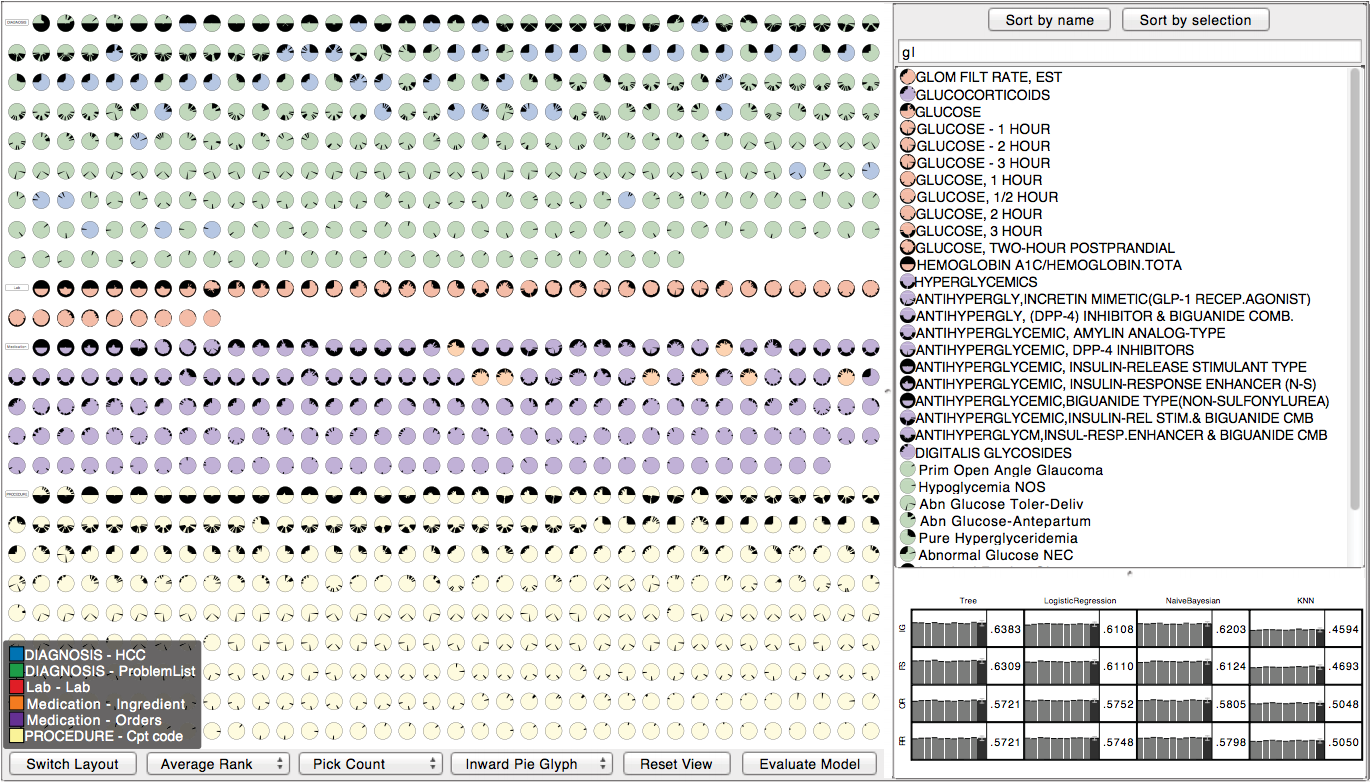
\includegraphics[width=0.8\linewidth]{figs/infuse/overview}
\caption{
The user interface of \textbf{INFUSE}.
}
\label{figs:infuse_overview}
\end{figure} %
% %\begin{figure}
\centering
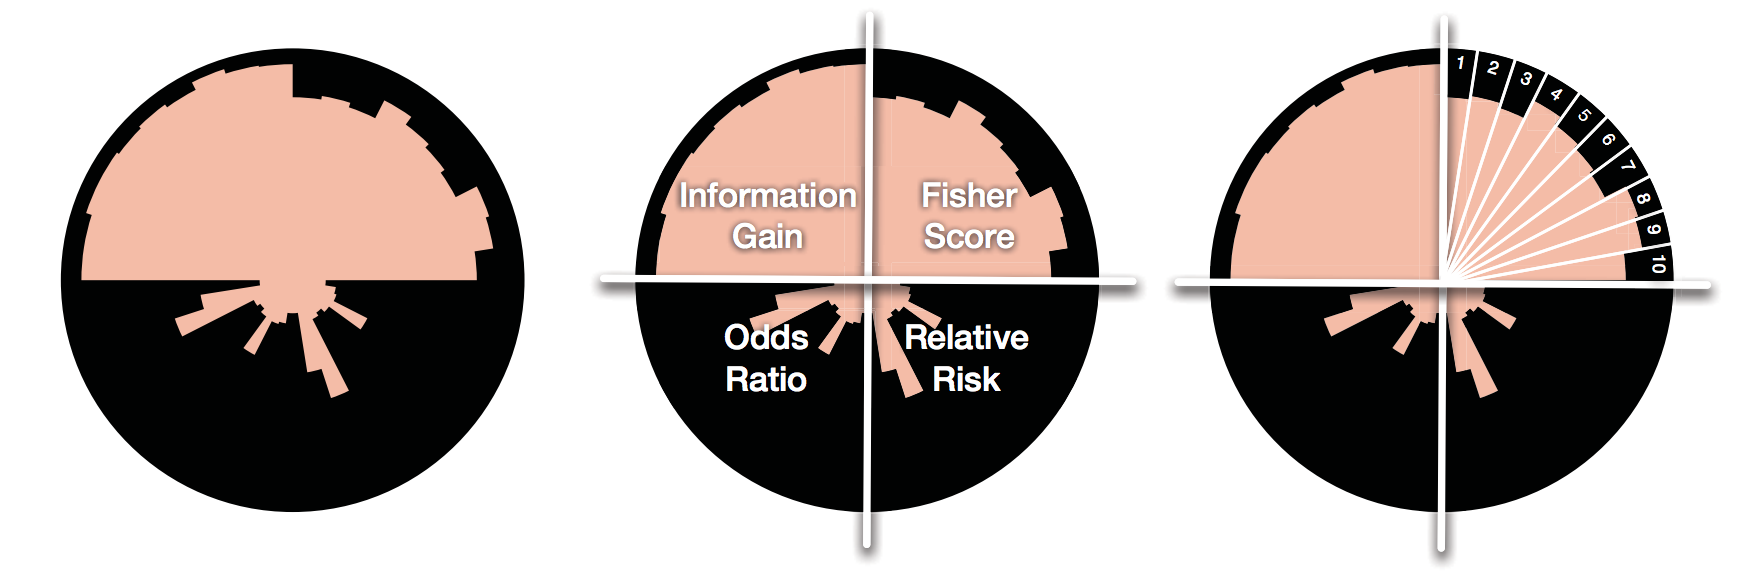
\includegraphics[width=\linewidth]{figs/infuse/reading}
\caption{
TODO
}
\label{figs:infuse_reading}
\end{figure} %\figref{figs:infuse_reading}
% %\begin{figure}
\centering
\includegraphics[width=\linewidth]{figs/infuse/findings}
\caption{
TODO
}
\label{figs:infuse_findings}
\end{figure} %\figref{figs:infuse_findings}

% \section{Class-Signatures: A Visual Analytics Workflow for Explanatory Analysis of Binary Classification Models}
% \label{sec:Class-Signatures}

% With \textbf{Class Signatures}, we propose a visual analytics workflow to interpret predictive associations between a large set of binary features and a binary target.
% For this we use a $4$ step pipeline: \textit{model}, \textit{contrast}, \textit{cluster}, and \textit{rank}, and a visual analytics interface that allows the end user to detect and interpret such associations.
% After modeling the predictive associations using a binary classifier we leverage the prediction scores with two user defined thresholds, one for positive cases and one for negative cases, to focus only on data items with a strong predictive signal, increasing contrast.
% Then, we cluster both positive and negative examples \textit{separately}.
% This groups together data points that have the same predicted outcome and a similar configuration of values.
% Finally, we rank each feature in the computed clusters using discriminative analysis across \textit{all clusters}.

% \begin{figure}[b!]
\centering
\includegraphics[height=13.5em]{figs/class_signatures/three_sides} % max 20em
\includegraphics[height=13.5em]{figs/class_signatures/class_signatures_only_no_side} % max 20em
\caption{
The user interface of \textbf{Class Signatures}.
}
\label{figs:class_signatures_overview}
\end{figure}

% For interpreting the results with visual analytics, we use \textbf{Class Signatures} as shown in \figref{figs:class_signatures_overview}.
% As our input features are binary in nature we show in the class signatures how consistently present
% a feature is in a cluster.
% This is indicated by bars growing both to the right (percentage of which feature is present) and the left (percentage of which feature is not present).
% In combination with the discriminative measure of the features (computed as gini-importance; the shade of feature backgrounds is visually encoded, so darker means more discriminative) users can formulate rules that explain predictions for different subgroups of data items.

% The proposed workflow allows for a more fine-grained analysis of the driving factors of a predictive task than using commonly used feature importance techniques.
% This is due to the observation that many phenomena have multiple underlying reasons for the same result.
% Thus an explanation is needed that distinguishes which features were actually responsible for given data points.
% \textbf{Class Signatures} provide this distinction in the form of user interpretable rules.

% Using \textbf{Class Signatures} to describe groups of patients admitted to the hospital
% because of different medications can be seen in \figref{figs:class_signatures_overview}.
% Each column represents one group (\emph{cluster}-step) whereas each row shows the amount of patients in this group taking a
% particular medication (the bar from the middle towards the right shows the percentage of patients taking the medication; the bar towards the left shows not taking medication).
% The color of the bar shows the distribution of the true outcome labels as found in the input data.
% The background of the rows shows the discriminativeness of a medication (dark being more discriminative \emph{wrt.} all other clusters; \emph{rank}-step).
% Above each group a \emph{t-SNE} projection of the items shows its relation to the other groups.
% ROC, precision-recall, and accuracy curves are shown on the left to facilitate selecting two thresholds to filter high signal patients (\emph{contrast}-step).

% \textbf{Class Signatures} has been published as work-in-progress as \cite{class_signatures}.
% The further plans for this project are outlined in \chapref{sec:Outlook}.
\chapter{Thesis Summary}
\label{chap:summary}

In this thesis, we discussed the role of visual analytics to explain black-box machine learning.
We saw that global approaches, like feature selection methods, are not informative enough to help understand model decisions.
Different strategies preferred different, equally reasonable, feature sets without having a significant impact on predictive performance.
This showed, that inspecting and comparing alternate settings may let machine learning experts develop insights that overwrite their initial intuitions.

Next, we saw that partial dependence with a derived feature importance score allowed to effectively detect model errors.
Detectable errors included: over-fitting, under-fitting, biases caused by imputation, and leaking labels caused by incorrect cause-effect relationships.
Furthermore, localized inspections helped to understand the how and why of specific instance predictions by finding locally impactful features.

Then, we proposed and discussed the Model Diagnostic workflow, which is based on aggregating local instance-level explanations in order to gain insights about a model with the intent of improving it.
We showed that the Model Diagnostic workflow enables a scalable understanding of local decision making of a predictive model and that aggregating instance-level explanations allows for semantic validation of the input data.
As a model can only perform as well as its input data, gaining insights about the limitations of a model in turn help with feature engineering on said data.

Finally, we showed how histograms can be effectively used to analyze aggregated instance-level explanations.
With the help of comparing meaningful subsets, aggregated instance-level explanations significantly outperformed inspecting individual explanations or aggregation without explanations in detecting biases in the input data while being more scalable than a tabular representation.
Furthermore, we showed that inspecting individual instance-level explanations can be misleading and hurts detecting biases in the input data.

All in all, we demonstrated a workflow for effectively utilizing black-box instance-level explanations in order to improve model correctness via semantic validation.
However, this approach has some limitations to overcome which we will explore next.
Note, that those limitations are not an argument against the presented techniques but merely a starting point for future research.

\section{Limitations and Assumptions of Black-Box Analysis}
Analyzing machine learning models using black-box techniques can only approximate the true behavior of the model.
Looking at more instances or increasing the sample rate for both partial-dependence plots or instance-level explanations increases the granularity and precision of the analysis but cannot express the underlying relationships of the input in full.
On the other hand, those relationships can be too complex to be understood by a human.
The challenge is to find a middle ground between the fidelity of explanations and their interpretability.

Additionally, some tasks have complex interactions between input features that cannot be described by interpreting individual features.
For example, instance-level explanations provide weights for the features for a given instance.
However, those weights can be completely different for other instances.
Instance-level explanations alone do not provide enough information to reason about why the weights changed in this particular way.
A possible solution could be to expand the concept of explanations to allow for representing non-trivial relationships between features, such as using rules to express partial behaviors of the model or a higher dimensional partial dependence.

Black-box analysis methods provide the convenience of using the same algorithm for multiple models.
However, with regards to data some decisions still need to be made.
For example, for the instance-level explanations in \chapref{chap:explainer} we determined that Martens and Provost's~\cite{Martens:2014:EDD:2600518.2600523} algorithm provided consistently better results than Riberio~\etal's\cite{DBLP:journals/corr/RibeiroSG16} algorithm for our use case of highly sparse binary data.
This is due to the fact that different data types require different approaches for explanations.
A binary feature can have an explanation that describes the presence or absence of the feature whereas for a numeric feature the actual value is important.
Our Model Diagnostic workflow is agnostic to the used instance-level explanation algorithm but this choice still has to be made.

\section{Generalization to Other Forms of Machine Learning}
In this thesis, we only focused on predictive modeling tasks with structured inputs.
Even though this is a large and popular subset, it does not cover the entirety of machine learning or even predictive modeling.
Presented techniques are not immediately transferable to tasks such as online learning or streaming input data, which requires recurrent models, such as LSTM (Long Short Term Memory) models~\cite{Hochreiter:1997:LSM:1246443.1246450}.
Those areas pose further challenges and offer a variety of research opportunities.

On a different note, the recent popularity of neural networks offers an additional opportunity in terms applicability of the work in this thesis.
Neural networks are differentiable models, which makes it possible to compute gradients towards desired outcomes for given inputs.
As instance-level explanations aim to approximate this gradient to some degree (LIME~\cite{DBLP:journals/corr/RibeiroSG16} is essentially a Monte-Carlo approximation of the above mentioned gradient) gradients might be used as drop-in replacements for instance-level explanations in the techniques proposed in this thesis.
However, whether gradients are a computationally faster alternative to instance-level explanations and whether they can achieve similar results poses an interesting open research question.

\section{Implications}
Meta-learning, \ie, using machine learning to learn model architectures for solving the actual task, is recently growing in popularity.
With systems, such as auto-sklearn~\cite{NIPS2015_5872} or AlphaGo~\cite{silver2016mastering}, the role of humans in machine learning shifts away from being the architect of models to being a domain expert of the modeled problem.
Humans have vast contextual knowledge that is hard to communicate directly to machine learning models.
As such, understanding the behavior of black-box machine learning models and semantic validation of their performance, as presented in this thesis, is becoming more and more relevant.

Interestingly, because humans are used to having contextual knowledge about real world problems machine learning is trying to solve, it often seems surprising when and why a model failed, since the correct prediction ``is so obvious".
% This also means, that repeatedly seeing that a model performs correctly, especially when providing a reasoning behind the decision in the form of \emph{explanations} might lead to overconfidence of the human in the capabilities of the model as we have seen in \chapref{chap:aggexplain}.
Thus, it is crucial for machine learning models to correctly communicate their behavior to humans in order to prevent such fallacies to go unnoticed.
This thesis provided an important step towards achieving this goal.

% \todo{see motivation for building context}
% \todo{discussion? -- also overfitting}
% \todo{end???}
% The model diagnostic workflow proposed in the previous chapter has so far only been tested with binary input features.
% This poses the question on how to expand to general numeric features.
% While it is possible to adapt the used explanation algorithm to accept arbitrary features the resulting explanations are less interpretable.

% \begin{figure}[t]
\centering
\includegraphics[height=16em]{figs/new_parallel.png}
\caption{
The extended interface to allow for non-binary data.
The list on the left shows the discovered ``decision sets".
Below that the distribution of prediction scores are shown.
A parallel coordinate view shows the instances covered by such a decision set (``expl 8") allowing non-binary input data.
The user highlights ``expl 10" showing its instances in purple.
}
\vspace*{-1em}
\label{figs:new_parallel}
\end{figure}
% \begin{figure}
\centering
\includegraphics[height=16em]{figs/new_multiclass.png}
\caption{
The extended design even allows for multi-class classification tasks.
The left shows the different ``decision sets" and how the prediction scores for a given class are distributed.
On the right the distribution of classes per feature are shown.
}
\label{figs:new_multiclass}
\end{figure}

% \section{Extending the Model Diagnostic Workflow}
% In the case of binary features just naming the feature is enough to show its significance and how it is used by the machine learning model.
% For numeric features additional information is needed.
% For example, an explanation would be ``Feature A has high values" which poses further questions of the granularity of the description (``Feature A $>$ 5", ``Feature A $>$ average").
% This introduces ambiguity and vagueness to the explanation.
% A possible solution to this is to describe the explanation \emph{implicitly} by showing the distribution of values within features and how features interconnect.
% The techniques proposed by \cite{seekaview} provide solutions to explore those relations effectively.

% Another problem arising from generalizing the model diagnostic workflow is the observation that explanation algorithms include more features when the features are numerical (\ie, more features are relevant to the prediction).
% The LIME algorithm \cite{DBLP:journals/corr/RibeiroSG16}, which produces feature weights for each instance, overcomes this issue by arbitrarily restricting features to a pre-chosen quantity (\eg, 10 features) by descending importance.
% This restriction is independent of the actual distribution of feature weights.
% It can happen that important features get removed or relatively unimportant features get included in the explanation.

% \begin{figure}
\centering
\includegraphics[height=22em]{figs/new_projection.png}
\caption{
Showing the distribution of instances according to the similarity of their explanations. The predicted label is also taken into account to allow for a clear separation of the two groups.
}
\label{figs:new_projection}
\end{figure}

% With the above mentioned shift away from \emph{explicitly} describing explanations through their features towards \emph{implicitly} describing explanations through their instances, less care has to be taken to keep the number of relevant features in a range that is interpretable.
% This opens up the aggregation of explanations from having explanations match exactly to being able to group together instances that are explained similarly.
% This can be achieved by clustering the feature weights as obtained from the LIME algorithm which solves the problem of arbitrarily cutting off features from explanations as all features are included in the distance metric for clustering.
% The resulting ``decision sets" can then be visualized (see Figures~\ref{figs:new_parallel}, \ref{figs:new_multiclass}, and \ref{figs:new_projection})
% \vspace*{-0.5em}

% \section{Formal Evaluation}
% The model diagnostic workflow proposed in \chapref{chap:explainer} has not been formally evaluated.
% We obtained information about its effectiveness through evidence from its use to improve machine learning models.
% However, this does not guarantee that using explanations for machine learning models actually have a positive impact on the human perception of the quality of a model.
% We are planning to run a study that aims to determine how the model diagnostic workflow changes the perceived trust and confidence in a model.
% Besides subjectively measuring trust and confidence we are presenting decisions made by a model alongside information about their underlying data and asking participants to decide whether the decision is correct.
% In one condition the participant has been exposed to only basic statistical performance measures of the machine learning models.
% In the other condition the participant has the opportunity to use an implementation of our model diagnostic workflow to gain deeper understanding into the strengths and weaknesses of the model.
% We have not started to run the study yet.

% The work shown so far provides an overview of how and where explanations of
% machine learning models can be helpful.
% However, it also shows gaps and challenges that provide much opportunity for further
% research.
% Especially for output only explanation there is still much room for improvements.
% Also, related research for interaction explanations
% (\cite{DBLP:journals/corr/RibeiroSG16} and \cite{Martens:2014:EDD:2600518.2600523})
% show a spectrum of different strategies on how to create those explanations but
% also show that there is still a lack of effective visual analytics tools conveying
% those explanations in a human understandable form.
% Two current projects address those challenges.

% \begin{figure}[b!]
\centering
\includegraphics[width=0.8\linewidth]{figs/current/paolo_explain}
\caption{
Interface for exploring explanations for data points.
}
\label{figs:paolo_explain}
\end{figure}

% \section{Current Projects}
% The first project, in collaboration with Paolo Tamag, addresses the visual analytics
% aspect of providing an effective user interface to explore and understand machine
% generated interaction explanations.
% The interface, shown in \figref{figs:paolo_explain},
% leverages the explanation generation strategy developed by
% \cite{Martens:2014:EDD:2600518.2600523} for explaining predictions
% in text classification tasks.
% It offers explanation exploration to find data points with similar reasons
% for their predicted outcome.
% In the interface the list on the left shows the terms most commonly occurring in explanations.
% After selection explanations containing the selected terms are shown in the middle
% column.
% Information about falsely predicted data points are shown as well.
% Explanations can be further inspected by listing all matching data points (right).
% Terms from the explanation are highlighted.
% Further work needs to be done to utilize the interplay of data driven clusters
% and explanation driven clusters.

% The second project aims to improve output only explanations.
% Here, only prediction scores are used to generate explanations.
% In the current state of the project paths towards the highest scoring item
% are computed on existing data points.
% The resulting tree graph structure can then be explored and used for
% explanation generation.
% This technique helps analysts find and understand clusters of similarly behaving
% data points and regions of great prediction score fluctuation in the item space.
% Initial experiments of visual analytics approaches can be seen in
% \figref{figs:current_adj},
% \figref{figs:current_graph}, and
% \figref{figs:current_burst}.
% Further work needs to be done in terms of summarizing groupings and guidance to
% interesting areas in the item space.

% \begin{figure}[b!]
\centering
\includegraphics[width=0.5\linewidth]{figs/current/graph_d2}
\caption{
Node-link diagram showing how neighborhoods of data points are interconnected
with increasingly larger distances.
The edges of the directed graph always lead to points with a higher prediction score.
Especially of interest are label flips (ie., the prediction score increases by a wide
margin) or neighborhoods with consistent labels.
}
\label{figs:current_graph}
\end{figure}

% \begin{figure}
\centering
\includegraphics[width=\linewidth]{figs/current/burst_d2_top}
\caption{
Isolated neighborhoods shown as sunburst charts.
Each segment represents one data point.
The center indicates the data point with the highest score.
The distance to the center roughly corresponds with the number of changes
to the feature vector that are necessary to turn a point into the point at the center.
The size of the segments corresponds to the amount of points ``flowing"
through a point towards the center.
}
\label{figs:current_burst}
\end{figure}

% \begin{figure}
\centering
\includegraphics[width=\linewidth]{figs/current/adj_top}
\caption{
Neighborhoods of data points.
Each row represents one neighborhood with its representative (the point with the
highest prediction score) shown on the right.
Each cell represents one data point of the neighborhood.
The background color indicates the prediction score.
The numbers show how many changes in the feature vector are necessary to turn the
point into the representative.
}
\label{figs:current_adj}
\end{figure}

% \chapter{Dissertation Outline and Progress}
% \label{chap:thesis}
% \section{Proposed Outline}
% Below is the proposed outline of the planned dissertation, with references to previous research.

% \begin{enumerate}[label*=\arabic*.]
%     \item Introduction
%     \begin{enumerate}[label*=\arabic*.]
%         \item Machine Learning
%         \begin{enumerate}[label*=\arabic*.]
%             \item Predictive Modeling
%             \item Popular Algorithms
%         \end{enumerate}
%         \item Motivation
%         \item Related Work
%         \item Use Case: Machine Learning for Health Care
%     \end{enumerate}
%     \item Feature Selection for Understanding Models
%     \begin{enumerate}[label*=\arabic*.]
%         \item INFUSE: Interactive Feature Selection for Predictive Modeling of High Dimensional Data (\textbf{publication}) ~\cite{infuse}
%         \item Context
%         \item Lessons Learned
%     \end{enumerate}
%     \item Partial Dependence for Understanding Models
%     \begin{enumerate}[label*=\arabic*.]
%         \item Prospector: Visual Inspection of Black-box Machine Learning Models (\textbf{publication}) ~\cite{prospector16}
%         \item Context
%         \item Lessons Learned
%     \end{enumerate}
%     \item Explanations for Understanding Models
%     \begin{enumerate}[label*=\arabic*.]
%         \item A Workflow for Visual Diagnostics of Binary Classifiers using Instance-Level Explanations (\textbf{publication}) ~\cite{explainer}
%         \item Context
%         \item Lessons Learned
%     \end{enumerate}
%     \item Generalization and Limitations of Explanations
%     \begin{enumerate}[label*=\arabic*.]
%         \item Generalization of Explanations to Non-Binary Data (\textbf{TBD})
%         \item Study on Impacts of Explanations for Model Confidence and Trust (\textbf{TBD})
%     \end{enumerate}
%     \item Discussion
%     \begin{enumerate}[label*=\arabic*.]
%         \item Limitations and Assumptions of Black-Box Analysis
%         \item Generalization to Other Forms of Machine Learning
%         \item Implications
%     \end{enumerate}
%     \item Conclusion and Future Work
% \end{enumerate}
% \newpage

\chapter{Conclusion \& Future Work}
\label{chap:future_work}

In this thesis we explored how visual analytics can be used in order to leverage the full potential of black-box machine learning.
To that extend we used a variety of techniques to explain the behavior of machine learning models, both globally and locally, and developed a workflow to utilize those explanations to diagnose model \todo{TODO}


%%%%% Appendices start %%%%%%%%%%%%%%%%
%% Comment out the following line if your thesis has no appendix
% \appendix
% \chapter{Appendix Chapter Title\label{chap:append}}

In the following we include ....


%% Note: If your thesis has more than one appendix, NYU requires a "list of
%% appendices" page before the body of the thesis. I don't provide the tools
%% to create that here, so you're on your own for that one... Sorry.
%\input{app2}

%%%% Input bibliography file %%%%%%%%%%%%%%%
% %% NYU PhD thesis format. Created by José Koiller 2007--2008.
%% Updated by Anshul Vikram Pandey with new design guidelines. 2017-2018

%% Use the first of the following lines during production to
%% easily spot "overfull boxes" in the output. Use the second
%% line for the final version.
\documentclass[12pt,draft,letterpaper]{report}
% \documentclass[12pt,letterpaper]{report}
% \documentclass[12pt]{article}

%% Replace the title, name, advisor name, graduation date and dedication below with
%% your own. Graduation months must be January, May or September.
\newcommand{\thesistitle}{USING~VISUAL~ANALYTICS~TO~EXPLAIN
BLACK-BOX~MACHINE~LEARNING}
\newcommand{\thesisauthor}{Josua Walter Hugo Krause}
\newcommand{\thesisadvisor}{Enrico Bertini, Ph.D.}
\newcommand{\graddate}{May 2018} % like January XX, May 20XX, September 20XX

%% If you do not want a dedication, scroll down and comment out
%% the appropriate lines in this file.
\newcommand{\thesisdedication}{To all the Ph.D. pursuing brave souls}

%% The following makes chapters and sections, but not subsections,
%% appear in the TOC (table of contents). Increase to 2 or 3 to
%% make subsections or subsubsections appear, respectively. It seems
%% to be usual to use the "1" setting, however.
\setcounter{tocdepth}{1}

%% Sectional units up to subsubsections are numbered. To number
%% subsections, but not subsubsections, decrease this counter to 2.
\setcounter{secnumdepth}{3}

% Setting a gap between page number and text block


%% Page layout (customized to letter paper and NYU requirements):
\setlength{\oddsidemargin}{.6in}
\setlength{\textwidth}{5.8in}
\setlength{\topmargin}{0.5in}
\setlength{\headheight}{0in}
\setlength{\headsep}{0in}
\setlength{\textheight}{8.3in}
\setlength{\footskip}{.5in}

%% Use the following commands, if desired, during production.
%% Comment them out for final version.
%\usepackage{layout} % defines the \layout command, see below
%\setlength{\hoffset}{-.75in} % creates a large right margin for notes and \showlabels

%% Controls spacing between lines (\doublespacing, \onehalfspacing, etc.):
\usepackage{setspace}

%
%% \usepackage{amsmath}
%% \usepackage{amssymb}
\usepackage{xspace}
\usepackage{algorithmic}
\usepackage{algorithm}
\usepackage{microtype}
% \usepackage{subfigure}
\usepackage{color}
\usepackage{url}
\usepackage{lipsum}
\usepackage{fancyhdr}
% \newfloat{algorithm}{t}{lop}

\pagestyle{fancy}
\fancyhf{}
\renewcommand{\headrulewidth}{0pt}
\fancyhead[L]{}
\fancyhead[R]{}
% \fancyhead[LE]{}
% \fancyhead[RO]{}
% \fancyhead[RE]{}
% \fancyhead[LO]{}
\fancyfoot[C]{}
\rhead{\thepage}

\fancypagestyle{plain}{%
\fancyhf{}
\rhead{\thepage}
}

\setlength{\headheight}{20pt} 

%% Use the line below for official NYU version, which requires
%% double line spacing. For all other uses, this is unnecessary,
%% so the line can be commented out.
\onehalfspacing % requires package setspace, invoked above

%% Each of the following lines defines the \com command, which produces
%% a comment (notes for yourself, for instance) in the output file.
%% Example:    \com{this will appear as a comment in the output}
%% Choose (uncomment) only one of the three forms:
%\newcommand{\com}[1]{[/// {#1} ///]}       % between [/// and ///].
\newcommand{\com}[1]{\marginpar{\tiny #1}} % as (tiny) margin notes
%\newcommand{\com}[1]{}                     % suppress all comments.

%% This inputs your auxiliary file with \usepackage's and \newcommand's:
%% It is assumed that that file is called "definitions.tex".
%%
%% Place here your \usepackage's. Some recommended packages are already included.
%%

% Graphics:
\usepackage[final]{graphicx}
%\usepackage{graphicx} % use this line instead of the above to suppress graphics in draft copies
%\usepackage{graphpap} % \defines the \graphpaper command

% Indent first line of each section:
\usepackage{indentfirst}

% Good AMS stuff:
\usepackage{amsthm} % facilities for theorem-like environments
\usepackage[tbtags]{amsmath} % a lot of good stuff!

% Fonts and symbols:
\usepackage{amsfonts}
\usepackage{amssymb}

\usepackage{xspace}
\usepackage{algorithmic}
\usepackage{algorithm}
\usepackage{microtype}
% \usepackage{subfigure}
\usepackage{color}
% \usepackage{todonotes}
\usepackage{url}
\newfloat{algorithm}{t}{lop}

% Formatting tools:
%\usepackage{relsize} % relative font size selection, provides commands \textsmalle, \textlarger
%\usepackage{xspace} % gentle spacing in macros, such as \newcommand{\acims}{\textsc{acim}s\xspace}

% Page formatting utility:
%\usepackage{geometry}
\usepackage{multirow}

%
\usepackage{listings}


%
\usepackage[numbers,sort]{natbib}

\usepackage[all,cmtip]{xy}

\usepackage{hyperref}
\hypersetup{
    colorlinks=true,
    linkcolor=blue,
    filecolor=blue,
    urlcolor=blue,
    citecolor=blue
}

% additional packages from proposal
% % \renewcommand{\familydefault}{\sfdefault}
% \usepackage[scaled=0.85]{beramono}
\usepackage{wrapfig}
% % \usepackage{caption}
\usepackage{subcaption}
\usepackage{tikz}
% \usepackage{natbib}
% % \usepackage[usenames,dvipsnames]{xcolor}
% % \usepackage{float}
% % \usepackage[rflt]{floatflt}
% \usepackage{hyperref}
% \hypersetup{
%     colorlinks = true,
%     allcolors = {black}
%     % citecolor = {blue},
%     % anchorcolor = {black}
% }

\usepackage{enumitem}
%%%

%%
%% Place here your \newcommand's and \renewcommand's. Some examples already included.
%%
%\newcommand{\acims}{\textsc{acim}s\xspace}
\newcommand{\Mspace}        {{\mathbb M}}
\newcommand{\Rspace}        {{\mathbb R}}
\newcommand{\Cspace}        {{\mathbb C}}

\newcommand{\Mo}        {{\hat M}}
\newcommand{\Ms}        {{\tilde M}}
\newcommand{\Do}          {{\hat D}}
\newcommand{\Ds}        {{\tilde D}}
\newcommand{\doo}          {{\hat d}}
\newcommand{\dss}        {{\tilde d}}
\newcommand{\w}        {{\mathbf w}}

% general
\newcommand{\reffig}[1]{{Figure~\ref{#1}}}
\newcommand{\refchap}[1]{{Chapter~\ref{#1}}}
\newcommand{\refsec}[1]{{Section~\ref{#1}}}
\newcommand{\reftab}[1]{{Table~\ref{#1}}}
\newcommand{\refapp}[1]{{Appendix~\ref{#1}}}
\newcommand{\refeq}[1]{{Equation~\ref{#1}}}
\newcommand{\refalg}[1]{{Algorithm~\ref{#1}}}
\newcommand{\myparagraph}[1]{\noindent \textbf{#1}}
\newcommand{\highlight}[1]{{\color{black}#1}}

\newcommand{\todo}[1]{\textcolor{blue}{[TODO] #1}\PackageWarning{definitions}{[TODO] #1}}
\newcommand{\expand}{\textcolor{green}{[EXPAND]}\PackageWarning{definitions}{EXPAND}}

\newcommand{\eg}{\emph{e.g.}\xspace}
\newcommand{\ie}{\emph{i.e.}\xspace}
\newcommand{\etc}{\emph{etc.}\xspace}
\newcommand{\wrt}{\emph{w.r.t.}\xspace}
\newcommand{\etal}{\emph{et~al.}\xspace}

\newcommand{\figref}[2][]{Figure~\ref{#2}#1\xspace}
\newcommand{\chapref}[1]{Chapter~\ref{#1}\xspace}
\newcommand{\secref}[1]{Section~\ref{#1}\xspace}
\newcommand{\infuse}{\emph{INFUSE}\xspace}

\newcommand{\prospector}{\emph{Prospector}\xspace}

\newcommand{\tabA}{Statistical Summary View\xspace}
\newcommand{\tabB}{Explanation Explorer\xspace}
\newcommand{\tabC}{Item Level Inspector\xspace}

\DeclareMathOperator*{\argmin}{arg\,min}
\DeclareMathOperator*{\argmax}{arg\,max}

% \newcommand{\ainfo}[1]{\phantom{#1}}
\newcommand{\ainfo}[1]{#1}

%%
%% Place here your \newtheorem's:
%%

%% Some examples commented out below. Create your own or use these...
%%%%%%%%%\swapnumbers % this makes the numbers appear before the statement name.
%\theoremstyle{plain}
%\newtheorem{thm}{Theorem}[chapter]
%\newtheorem{prop}[thm]{Proposition}
%\newtheorem{lemma}[thm]{Lemma}
%\newtheorem{cor}[thm]{Corollary}

%\theoremstyle{definition}
%\newtheorem{define}{Definition}[chapter]

%\theoremstyle{remark}
%\newtheorem*{rmk*}{Remark}
%\newtheorem*{rmks*}{Remarks}

%% This defines the "proo" environment, which is the same as proof, but
%% with "Proof:" instead of "Proof.". I prefer the former.
%\newenvironment{proo}{\begin{proof}[Proof:]}{\end{proof}}


%% Cross-referencing utilities. Use one or the other--whichever you prefer--
%% but comment out both lines for final version.
%\usepackage{showlabels}
%\usepackage{showkeys}
% \pagestyle{headings}

\begin{document}
%% Produces a test "layout" page, for "debugging" purposes only.
%% Comment out for final version.
%\layout % requires package layout (see above, on this same file)
%% Sets page numbering to "roman style" i, ii, iii, iv, etc:

%%%%%% Cover page %%%%%%%%%%%
%% Sets page numbering to "roman style" i, ii, iii, iv, etc:
\pagenumbering{roman}
\thispagestyle{empty}
\begin{center}
{\bfseries 
  {\large\thesistitle}
  \vspace{1in}
  
 {\large {\bf DISSERTATION}}\\
  \vspace{.5in}
  
  \begin{doublespace}
  {\large  
  Submitted in Partial Fulfillment of\\
  % \vspace{.1in}
  the Requirements for\\
  % \vspace{.1in}
  the Degree of\\}
  \end{doublespace}
  \vspace{.5in}
  
  {\large DOCTOR OF PHILOSOPHY (Computer Science)}\\
  \vspace{.5in}
  
  at the \\
  \vspace{.2in}
  
  {\large
  NEW YORK UNIVERSITY\\
  \vspace{-0.05in}
  TANDON SCHOOL OF ENGINEERING\\
  }
  \vspace{.2in}
  
  by
  \vspace{.5in}

  {\large\thesisauthor}
  \vspace{.5in}
  % \vfill

  {\large\graddate}
}

\end{center}

\newpage

%%%%%% Title page %%%%%%%%%%%
%
\setcounter{page}{1}
%% No numbering in the title page:
\thispagestyle{empty}
%
\begin{center}
{\bfseries 
  {\large\thesistitle}
  \vspace{.25in}
  
  DISSERTATION\\
  \vspace{.25in}
  
  \begin{doublespace}
  Submitted in Partial Fulfillment of\\
  % \vspace{.1in}
  the Requirements for\\
  % \vspace{.1in}
  the Degree of\\
  \end{doublespace}
  \vspace{.25in}
  
  DOCTOR OF PHILOSOPHY (Computer Science)\\
  \vspace{.25in}
  
  at the \\
  \vspace{.1in}
  
  {\large
  NEW YORK UNIVERSITY\\
  \vspace{-0.05in}
  TANDON SCHOOL OF ENGINEERING\\
  }
  \vspace{.2in}
  
  by
  \vspace{.3in}

  \thesisauthor
  \vspace{.3in}
  % \vfill

  \graddate
}

\end{center}
% \vfill

\vspace{0.2in}

\noindent
\makebox[\textwidth]{\hfill\makebox[2.5in]{Approved: \hfill}}
\vspace{0.1in}

\noindent
\makebox[\textwidth]{\hfill\makebox[2.5in]{\hrulefill}}\\
\makebox[\textwidth]{\hfill\makebox[2.5in]{\hfill Department Head Signature\hfill}}
\vspace{0.05in}

\noindent
\makebox[\textwidth]{\hfill\makebox[2.5in]{\hrulefill}}\\
\makebox[\textwidth]{\hfill\makebox[2.5in]{\hfill Date \hfill}}

\noindent
Copy No.\hspace{33pt} \noindent\rule[-3pt]{2in}{0.4pt}\\
University ID\#:      \noindent\rule[-3pt]{2in}{0.4pt}\\

%\newpage

%%%%%%%%%%%%%% Copyright Page %%%%%%%%%%%%%%%%%

%%%%%%%%%%%%%% Guidance Committee Signature Page %%%%%%%%%%%%%%%%%
Approved by the Guidance Committee:
\singlespacing

\underline{Major}: Computer Science
\vspace{0.7in}

\noindent
\makebox[\textwidth]{\hfill\makebox[3in]{\hrulefill}}\\
\makebox[\textwidth]{\hfill\makebox[3in]{\hfill \textbf{Advisor's Name}\hfill}}
\makebox[\textwidth]{\hfill\makebox[3in]{\hfill Professor of \hfill}}
\makebox[\textwidth]{\hfill\makebox[3in]{\hfill Computer Science and Engineering \hfill}}
\makebox[\textwidth]{\hfill\makebox[3in]{\rule[-4pt]{2in}{1pt}}}\\
\makebox[\textwidth]{\hfill\makebox[3in]{\hfill Date \hfill}}\\
\vspace{0.5in}

\noindent
\makebox[\textwidth]{\hfill\makebox[3in]{\hrulefill}}\\
\makebox[\textwidth]{\hfill\makebox[3in]{\hfill \textbf{Advisor's Name}\hfill}}
\makebox[\textwidth]{\hfill\makebox[3in]{\hfill Professor of \hfill}}
\makebox[\textwidth]{\hfill\makebox[3in]{\hfill Computer Science and Engineering \hfill}}
\makebox[\textwidth]{\hfill\makebox[3in]{\rule[-4pt]{2in}{1pt}}}\\
\makebox[\textwidth]{\hfill\makebox[3in]{\hfill Date \hfill}}\\
\vspace{0.5in}


\noindent
\makebox[\textwidth]{\hfill\makebox[3in]{\hrulefill}}\\
\makebox[\textwidth]{\hfill\makebox[3in]{\hfill \textbf{Advisor's Name}\hfill}}
\makebox[\textwidth]{\hfill\makebox[3in]{\hfill Assistant Professor of \hfill}}
\makebox[\textwidth]{\hfill\makebox[3in]{\hfill Computer Science and Engineering \hfill}}
\makebox[\textwidth]{\hfill\makebox[3in]{\rule[-4pt]{2in}{1pt}}}\\
\makebox[\textwidth]{\hfill\makebox[3in]{\hfill Date \hfill}}\\
\vspace{0.5in}

\noindent
\makebox[\textwidth]{\hfill\makebox[3in]{\hrulefill}}\\
\makebox[\textwidth]{\hfill\makebox[3in]{\hfill \textbf{Advisor's Name}\hfill}}
\makebox[\textwidth]{\hfill\makebox[3in]{\hfill Assistant Professor of XXX\hfill}}
\makebox[\textwidth]{\hfill\makebox[3in]{\hfill Computer Science and Engineering \hfill}}
\makebox[\textwidth]{\hfill\makebox[3in]{\rule[-4pt]{2in}{1pt}}}\\
\makebox[\textwidth]{\hfill\makebox[3in]{\hfill Date \hfill}}\\

\doublespacing

%%%%%%%%%%%%%% Microfilm / Publishing Page %%%%%%%%%%%%%%%%%
\begin{center}
Microfilm or other copies of this dissertation are obtainable from
\vspace{4in}

UMI Dissertation Publishing\\
ProQuest CSA\\
789 E. Eisenhower Parkway\\
P.O. Box 1346\\
Ann Arbor, MI 48106-1346

\end{center}
\newpage

%%%%%%%%%%%%%% Vita %%%%%%%%%%%%%%%%%
\section*{Vita}
\addcontentsline{toc}{section}{Vita}
%!TEX root = thesis.tex

\todo{TODO}
Your vita goes here. This is usually a paragraph or two. Be careful about what you write here. :)

\lipsum[1]
\newpage



%%%%%%%%%%%%%% Ackknowlegment %%%%%%%%%%%%%%%%%
%% Comment out the following lines if you do not want to acknowledge
%% anyone's help...
\section*{Acknowledgements}
\addcontentsline{toc}{section}{Acknowledgements}
%!TEX root = thesis.tex

%% Write your acknowledgements in this file. If you do not want to acknowledge anyone,
%% you can delete this file and comment out the corresponding part in the "thesis.tex"
%% file.
\lipsum[1]

\noindent
\makebox[\textwidth]{\hfill\makebox[3in]{\hfill Your Name\hfill}}
\makebox[\textwidth]{\hfill\makebox[3in]{\hfill\graddate\hfill}}


\newpage

%%%%%%%%%%%%%% Dedication Page %%%%%%%%%%%%%%%%%
%% Comment out the following lines if you do not want to dedicate
%% this to anyone...
\vspace*{\fill}
\begin{center}
  \thesisdedication%\addcontentsline{toc}{section}{Dedication}
\end{center}
\vfill
\newpage


%%%%%%%%%%%%%% Abstract %%%%%%%%%%%%%%%%%
\section*{}
\begin{center}
{\bfseries 
  %{\large\thesistitle}
  \vspace{.25in}  
  {\bf ABSTRACT}\\
  \vspace{.25in}
  {\bf \thesistitle}\\  
  \vspace{.25in}
  {\bf by}\\  
  \vspace{.5in}
  {\bf \thesisauthor}\\
  \vspace{.5in}
  {\bf Advisor: Prof. \thesisadvisor}\\
  \vspace{.25in}
  {\bf Submitted in Partial Fulfillment of the Requirements for}\\
  {\bf the Degree of Doctor of Philosophy (Computer Science)}\\
  \vspace{.25in}
  {\bf \graddate}  
  \vspace{.25in}
}
\end{center}
\addcontentsline{toc}{section}{Abstract}
% \begin{abstract}
\todo{refine / update}
As machine learning models increase in complexity, the human ability of understanding and interpreting decisions made by those models has not been able to keep up.
The usefulness of white-box analysis techniques, exposing the internal state of models, are limited to relatively simple models and have trouble with complex models, such as deep neural networks.
Recently, black-box machine learning analysis techniques offer model independent insights into the decision making process of machine learning models.
For quickly and effectively gaining insights from those techniques, visual analytics emerges as a powerful set of tools.
We use visual analytics to explore both global and local means of explaining and understanding predictive models via black-box techniques.
We then propose a model diagnostic workflow that uses aggregated instance level explanations to overcome problems of fully global or local methods.
That is, by avoiding global aggregates, finer details of the decision making process are retained, while going beyond individual instances, analysts are not overwhelmed by the quantity of instances to inspect.
Finally, we show that the model diagnostic workflow can not only help improving the models themselves but offers insights about flaws in the \emph{input data}, thus helping with the task of feature engineering.

% With the increasing complexity of modern machine learning the need for
% transparency in its decision making emerges.
% This need extends beyond simple statistical performance measure, like precision or
% accuracy, since those metrics do not provide information about the validity of the
% decision making process.
% Explanations offer an insight in the reasoning of a machine learning model
% that can be enhanced substantially using visual analytics.
% In this work we explore several approaches on how visual analytics can benefit
% transparency using explanations for predictive modeling, a discipline of machine learning.
% Utilizing different aspects of the predictive modeling pipeline, namely using the input,
% the output, and input-output model interactions those explanations can be created in a
% model agnostic black-box fashion.
% We conclude with current in-progress research projects.

% \textbf{Keywords:}
% Visual Analytics,
% Visualization,
% Predictive Modeling,
% Explanations,
% Machine Learning,
% Black-box
% \end{abstract}
\newpage

%%%% Table of Contents %%%%%%%%%%%%
\tableofcontents
% \clearpage
% \pagestyle{headings}

%%%%% List of Figures %%%%%%%%%%%%%
%% Comment out the following two lines if your thesis does not
%% contain any figures. The list of figures contains only
%% those figures included withing the "figure" environment.
\listoffigures\addcontentsline{toc}{section}{\listfigurename}
\newpage

%%%%% List of Tables %%%%%%%%%%%%%
%% Comment out the following two lines if your thesis does not
%% contain any tables. The list of tables contains only
%% those tables included withing the "table" environment.
\listoftables\addcontentsline{toc}{section}{\listtablename}
\newpage

%%%%% Body of thesis starts %%%%%%%%%%%%
\pagenumbering{arabic} % switches page numbering to arabic: 1, 2, 3, etc.

%% Introduction. If your thesis has no introduction, or chapter 1 is
%% meant to be the introduction, then comment out the lines below.
%% \section*{Introduction}\addcontentsline{toc}{section}{Introduction}
%\input{intro}

%%If your thesis has different "Parts", use commands such as the following:
\chapter{Introduction}
\vspace*{-2em}
In computer science, machine learning is a set of methods for learning models from examples that accurately perform tasks on new or unseen data without explicitly codifying all instructions. This automation of programming provides a time- and cost-effective alternative to otherwise manually created software solutions, making machine learning popular and widely used for many applications.

However, the relative lack of human supervision in their creation makes it hard to fully understand the inner workings of trained models and limits the ability to verify that the models work correctly. Even though it is possible to statistically verify the correctness of a model by testing it against an unseen dataset whose ground truth is known, models can unknowingly utilize latent variables that should not be used. Knowledge about those factors is often implicit in the domain of the task and neither encoded in the data nor the model. Human expertise is needed to detect and encode them explicitly or to block them out.

For example, Caruana~\etal\cite{Caruana:2015:IMH:2783258.2788613} built a Generalized Additive Model with pairwise interaction ($GA^2M$) to predict mortality risk for hospitalized patients with pneumonia, a potentially life-threatening lung infection. This area of machine learning is called predictive modeling and uses machine learning to predict a certain outcome, in this case mortality risk, based on values of several input features, in this case laboratory measurements, comorbidities, or patient demographics, and is trained from and applied to many instances. It is not feasible to individually check each prediction of the model manually. However, the machine learning algorithm $GA^2M$ used for this study is an intelligible model, that sacrifices parts of its predictive quality in favor of being understandable by humans. This enabled the authors to inspect how features contributed to the predicted outcome. One of their findings was that the model associated having asthma, a chronic lung disease, with a lower mortality rate for pneumonia patients. However, this combination of diseases is known to have a significantly \emph{increased} mortality rate. The authors double checked their data and found that this phenomenon actually occurred in their dataset and thus appeared as correct prediction in their model. After further investigation it became clear that this bias in the dataset stemmed from patients, with those conditions, being treated with intensive care thus lowering their mortality risk below the average. Outside of a hospital the risk of those patients would have been significantly higher. The model, however, only learnt about hospitalized patients which led to it being confident in this false association.

The above example illustrates the need for human understanding and supervision in machine learning and the incorrect correct result could easily be identified since the authors used a special, intelligible, model. However, not all models used in machine learning are, or even attempt to be, easily interpretable by human experts. To counteract this, visual analytics has been successfully used to visualize machine learning processes in order to understand and gain insights into predictive models. Visual analytics is the area of studying interactive graphical representations of abstract information with the help of computational and statistical procedures, in order to effectively analyze complex data. With regards to understanding the decision making of predictive machine learning models, there are two main strategies: white-box and black-box analysis \cite{class_signatures}.

% \section{White-box vs. Black-box Analysis}
In white-box analysis the main focus lies in communicating the internal structure of the model at hand. That is, the analysis is based on the assumption that knowing the full internal state of a model and being able to manually retrace decisions made by it, helps understanding the \emph{behavior} of the model in general.

In this work we will focus on black-box analysis whose focus is on communicating external behavior of a model. That is, no information about the model itself is utilized during the analysis but rather typically inferred from observing how the model reacts to carefully crafted inputs. Compared to white-box analysis there are several advantages.

As white-box analysis relies on the internal structure and thus the nature of a particular model type, such as the $GA^2M$ mentioned above, a method developed for one type might not be applicable to a different type. This limits the usefulness of white-box analysis as every new algorithm demands often an entirely new form of representation. Since black-box analysis is model independent findings are universally applicable.

\newcommand\Tstrut{\rule{0pt}{2.5ex}}
\begin{table}
     \begin{tabular}{cl|cl} 
     & \textbf{White-box} & & \textbf{Black-box} \\
     \hline
     \hline
    $\oplus$ & Deep understanding of decisions & $\ominus$ & External behavior only \Tstrut \\
    $\oplus$ & Always reflects the true & $\ominus$ & Not guaranteed to reflect model \Tstrut \\
    & decision making process & & decisions truthfully in all cases \\
    $\oplus$ & Full internal state available & $\ominus$ & Limited knowledge of \Tstrut \\
    & & & model specifics \\
    \hline
    $\ominus$ & Model specific techniques & $\oplus$ & Reusable techniques \Tstrut \\
    $\ominus$ & Complexity / interpretability & $\oplus$ & Complexity / interpretability \Tstrut \\ 
    & data and model dependent & & independent of data and model \\
    $\ominus$ & Switching to interpretable model & $\oplus$ & No performance considerations \Tstrut \\
    & incurs performance penalty & & necessary \\
    \end{tabular}
    \centering
    \vspace*{-0.5em}
    \caption{Comparison of black-box and white-box explanation strategies. $\oplus$ indicates advantages of a technique while $\ominus$ indicates drawbacks.}
    \vspace*{-0.75em}
    \label{tab:blackvswhite}
\end{table}

Another drawback of white-box analysis is its scalability to the complexity of the model. Many solutions do not sufficiently scale as models become more complex. For example, a decision tree with 5 nodes, often used as example when explaining the technique, can easily be visualized and understood in a node-link representation. This representation fails to help understanding a decision tree with hundreds or thousands of nodes. For black-box analysis the internal complexity of a model is irrelevant.

On the other hand black-box analysis also has drawbacks. Especially the limited knowledge of the underlying model allows only for an approximate understanding of its behavior as testing the entire input space would be intractable.

The main goal of this thesis is to explore how model agnostic feature contribution methods can help to gain a holistic understanding of, as well as, insights about predictive models using visual analytics. In three stages, we will show the progression from initial observations, that led us to utilizing black-box analysis, to the eventual use of aggregated instance-level explanations to understand, trust, and verify predictive models. Additionally, we show that our developed visual analytics techniques can be helpful for feature engineering.

Feature engineering is the task of deciding which features will be collected for a particular machine learning problem and how those features are pre-processed or transformed in order to create favorable model results. It requires both expertise of the problem domain, as well as, experience in picking and manipulating features in ``the right way". For the most part, feature engineering cannot be automated and is typically seen as ``black-art" as it relies on intuition and creativity of the modeler \cite{Domingos:2012:FUT:2347736.2347755}.

% \section{\infuse}
In the first stage we analyze and compare different feature selection strategies. Feature selection is a pre-processing step that, unlike feature engineering, algorithmically determines the possible predictive impact of a feature. Only the most impactful features are then used as input for the predictive modeling process. This is often necessary as a larger number of features require significantly more training examples to accurately represent the valid input space without losing predictive qualities. As feature selection algorithms use similar statistical tools as many predictive modeling techniques it seems plausible to infer the importance of features in the context of decision making through feature selection in a model agnostic way.

Being able to visually compare different feature selection strategies the machine learning experts noticed that, depending on the chosen feature selection algorithm, different, mostly distinctive, feature sets were deemed to be important while, at the same time, having no significant impact on predictive performance. Additionally, from the view of a domain expert those feature sets were equally reasonable in the context of the prediction task.
This demonstrates that \textbf{inspecting} and \textbf{comparing alternate settings} lets machine learning experts develop insights that \textbf{overwrite} their \textbf{initial intuitions}.
Also, concluding that rankings from feature selection algorithms are not informative enough to provide the importance of features in the context of understanding model decisions, a more powerful model agnostic approach is needed.

% \section{\prospector}
In the second stage we explore the influence of features in the decision making process of predictive models through a technique called partial dependence. Partial dependence computes feature impact on model outcomes by systematically probing the model with artificial inputs. That is, while keeping the rest of the input values the same, the inspected feature assumes all possible values showing the relationship of feature values to the prediction score. Aggregated over all observed instances, the general behavior of the model with respect to a given feature can be inferred. By computing a novel feature importance score from partial dependence relationships unusual and interesting relations can be found quickly without having to inspect all, often several thousand, features.

Analyzing partial dependency relationships on diabetes prediction models trained on electronic medical records containing patient demographics, diagnoses, medications, and laboratory results, using our method we gained several insights. Firstly, we showed that logistic regression models are not expressive enough to accurately model the complex relationships of certain features to the outcome. Secondly, imputation of missing values, using the population average in laboratory results, caused the model to become uncertain close to the normal value range of laboratory tests. Lastly, we found that the model used a proxy variable indicating the number of doctor visits as predictor of the healthiness of a patient. However, this is \emph{not} a valid predictor. Even though a patient is likely to visit a doctor more often if she is sick, the reverse cannot be said. The above findings show how \textbf{partial dependence} with the proposed \textbf{feature importance score} allow analysts to effectively \textbf{detect model errors} related to \textbf{over-} and \textbf{under-fitting}, \textbf{imputation}, and \textbf{incorrect cause-effect relationships}.
However, a major drawback of using partial dependency is its limitations on extending it to relations of multiple features to the predicted outcome.

\begin{figure}[t]
\centering
\includegraphics[width=\textwidth]{figs/workflow_large}
\caption[The model diagnostic workflow.]{
The proposed \textit{model diagnostic} workflow extends the conventional \textit{model building} workflow in machine learning for enabling domain experts to reason about the semantic validity of the decisions made by any model through multiple linked visualizations.
This ultimately helps to improve data acquisition and model generation processes belonging to the original workflow.
}
\label{figs:workflow_intro}
\end{figure}

% \section{Model Diagnostic Workflow}
In the third stage, we overcome this limitation by leveraging instance-level explanations. Instance-level explanations are defined as the smallest change, to an instance vector, necessary to change the predicted outcome label. Aggregating over those explanations and statistically analyzing the resulting instance subsets, proves as powerful novel approach for understanding the behavior of a model. Additionally, we propose a model diagnostic workflow (see \figref{figs:workflow_intro}) that helps identify flaws in the \emph{input data}, used to train and test the model.

We use this workflow to analyze a predictive modeling problem revolving patient admission to a hospital, of patients in the emergency department of said hospital. Accurately predicting whether a patient eventually gets admitted to the hospital helps reducing costs. The major limiting factor of this prediction task is the need for input features readily, and electronically, available at the earliest point possible. To this extend we initially used features of prescribed medications as this information is immediately available electronically. Our analysis showed that there are clear groups of patients where the predictive model is very helpful. However, there are some groups of patients where it is impossible for the predictive model to make accurate predictions given the provided information. One of those groups is patients receiving Diatrizoate Meglumine, a contrast medium for CAT or PET scans. This medication only indicates that a scan was performed, but does not carry information about the result of the scan. However, the result of the scan is the deciding factor whether a patient needs further care or can get sent home. Thus, with the given information it is impossible for the predictive model to make a decision that performs better than random guessing. Including more information in the form of additional features does indeed help with this problem but pushes the time when a decision can be made further back. One possible solution is to utilize the predictive model only for the confident groups of patients and wait for the doctors' decisions in other cases. This example illustrates that it is not only possible to \textbf{understand decision making} of a predictive model through the \textbf{model diagnostic workflow} based on \textbf{aggregated instance level explanations}, but also how it can be applied for \textbf{semantic validation} and \textbf{feature engineering} on the input data.

\begin{table}[t]
     \begin{tabular}{l|c|c|c} 
     \textbf{Approach} & \makebox[0pt][l]{\textbf{Instances}}\phantom{Aggregated} & \textbf{Aggregated} & \makebox[0pt][l]{\textbf{Global}}\phantom{Aggregated} \\ 
     \hline
     \hline
     \infuse & & & X \Tstrut\\
     \hline
     \prospector & X & & X \Tstrut\\
     \hline
     \textit{Model diagnostic workflow} & & X & \Tstrut\\
    \end{tabular}
    \centering
    \vspace*{-0.5em}
    \caption{Locality of decision analyses of the presented approaches. \textbf{Instances} refers to analyzing decisions for one instance at a time. \textbf{Aggregated} refers to analyzing decisions for groups of instances and \textbf{Global} refers to analyzing decisions globally without inspecting decisions for individual instances.}
    \vspace*{-0.75em}
    \label{tab:locality}
\end{table}

\todo{fill in latest work}
In addition to those promising results, there is still work to do.
It still needs to be shown that the proposed workflow of statistical analysis of instance-level explanations can be successfully applied to other data types than binary feature vectors, such as numerical features or highly redundant features such as found in images.
Early results in this direction indicate that it might be beneficial to abandon the focus on features to explain machine learning models, but rather focus on instances directly.
That is using instance-level explanations to obtain groups of \emph{instances} with similar behavior and then visualize those groups (\eg, using techniques proposed by \cite{seekaview}) in order to \emph{implicitly} explain them.
This provides more flexible explanations than those proposed earlier as their capability goes beyond ``Feature A and feature B positively impact the prediction for this group of instances" to also allow insights of the form ``The number of circles formed by black pixels contribute positively to the prediction" which would be very difficult to formulate by a machine but are easily formulated by humans using visualizations.
Furthermore, we are going to run a study on the implications on confidence in and trust of machine learning models when using different explanation approaches.
\todo{END?}

%%%
%  Furthermore, a formalization or taxonomy of common machine learning modeling \emph{errors} in both the modeling and feature engineering steps is needed to fully determine the limitations of the proposed black-box analysis methodologies. This can be achieved by taking a survey with both machine learning and domain experts to get an understanding and relevance of different kinds of those errors.
%%%

% Machine learning is a powerful tool that is used more and more in everyday life.
% By relating independent features and targets by detecting complex associations machine learning
% helps human decision making and, in some cases, even replaces it.
% Predictive modeling using classification techniques is a very common application of machine learning.
% In this work we will primarily focus on classification but the techniques discussed can, to some extent, be
% applied in other areas of machine learning as well.

% \begin{figure}
\centering
\vphantom{7cm}
\includegraphics[trim={7cm 8cm 7cm 8cm},clip=true,width=0.275\linewidth]{figs/motivation/hmr}
~
\includegraphics[trim={7cm 8cm 7cm 8cm},clip=true,width=0.275\linewidth]{figs/motivation/hmr_complex}
~
\includegraphics[trim={7cm 8cm 7cm 8cm},clip=true,width=0.275\linewidth]{figs/motivation/hmr_interpretable}
\caption{
Humans (lower left) build machine learning models (top) to understand and
predict reality (lower right). The second image illustrates how improving
machine learning models (ie., closing the gap between the model and reality)
makes it harder for humans to understand it. Likewise, simplifying the model
(ie., closing the gap between the model and the human) makes the model less
accurate (third image).
}
\label{figs:motivation_hmr}
\end{figure}

% As the scope and usage of machine predictions increases with bigger and more complex data
% the used algorithms need to also become more complex.
% However, as complexity increases it becomes harder for humans to follow the machine's decision making
% as illustrated in \figref{figs:motivation_hmr}.
% This problem of model transparency and interpretation is important and very well recognized in machine learning,
% as models with high predictive performance generally have low transparency and vice-versa~\cite{breiman2001}.

% \begin{figure}
\centering
\includegraphics[height=10.5em]{figs/motivation/ml_orig}
\raisebox{4.75em}{$\Rightarrow$}
\includegraphics[height=10.5em]{figs/motivation/ml_proj}
\caption{
Machine learning algorithms transform the complex raw input space (left)
into a cleaner transformed space (right) that can be easily separated.
Transformations are often strongly non-linear, non-affine, and/or non-continuous
and thus not easy to follow or understand.
}
\label{figs:motivation_ml}
\end{figure}

% Many applications of machine learning need to be interpretable to humans even though
% sacrificing prediction performance is not desirable.
% For example, in the health care domain disease prediction using patient histories needs to be fully
% transparent and comprehensible to practitioners as lives are at stake when applying models in the real world.
% Even if a model performs well on the test data it could draw its conclusions from hidden signals or biases
% in the training data. We found many of such examples in the work presented here.

% One way of overcoming the problem of interpretability vs. performance in machine learning is to
% break down the complex models into smaller parts that are easier to understand (see \figref{figs:motivation_ml}).
% While this reduces the complexity it also reduces the generalizability of the explanations created this way.
% In the following we will explore when explanations are useful and how they can be used.

% \section{Explanations}
% Explanations for machine learning can be desirable for multiple reasons:

% \begin{description}
%     \item[Liability]
%         Decisions made by the machine have real world consequences with attached liabilities.
%         Explanations are needed to create confidence that the model avoids costly misjudgements of critical inputs.
%     \item[Trust]
%         Stakeholders need to be able to trust decisions from the model.
%     \item[Debugging]
%         Help understanding why a model behaves different than expected.
%     \item[Comparison]
%         Provide a model agnostic way of comparing different models.
%     \item[Hidden Associations]
%         Find hidden associations in the original data.
%     \item[Ambiguity Reduction]
%         By creating generalizing models and explaining their behavior a noise-free view of the data can be created.
% \end{description}

% Those explanation tasks can be performed at different steps in the machine learning process.
% In this context predictive modeling typically consists of three steps (see \figref{figs:motivation_flow}).
% First, the input data has to be prepared.
% This entails choosing which data points are eligible for modeling to ensure that no inherent biases influence
% the validity of the created model.
% Furthermore, data usually needs to be converted into features that can be used by machine learning models.
% Second, the model has to be trained on the transformed data.
% Depending on the type of the model or strategy this step includes splitting the data into cross-validation sets,
% algorithmic feature selection, and actually training the model.
% Third, the actual prediction can be performed which often entails converting class probabilities into
% concrete labels upon which decisions can be performed.

% Explanations can be separated into different categories that utilize and describe
% different stages of the predictive modeling pipeline.
% Thus, explanations can be divided into input-, output-, interaction-,
% and structure-explanations.
% Input explanations mostly work with the raw input data and can help the pre-processing.
% Output explanations analyze outputs from the machine learning model such as feature ranks
% or prediction scores.
% Interaction explanations change model inputs to observe how the corresponding model output
% changes.
% Structure explanations describe the inner values and weights of a model so decisions
% can be followed manually.

% \begin{figure}[b!]
\centering
\includegraphics[width=0.7\linewidth]{figs/motivation/flow}
\caption{
The predictive modeling pipeline.
Humans symbolize where explanations are helpful.
Explanations of the model can either focus on input-output interactions
or the structure of the model.
}
\label{figs:motivation_flow}
\end{figure}

% Output and interaction explanations can also utilize model induction, which is building
% a less complex model on top of the original model's output or on a strategically chosen
% subset of data points.
% This less complex model can then be structurally described which is beneficial when
% dealing with very complex models whose structural explanations are too difficult to
% understand.

% \begin{figure}
\centering
\includegraphics[height=11em]{figs/motivation/expl_classes}
\caption{
The relation of output-, interaction-, and structure-explanations.
With the help of model induction over a reduced or carefully selected
input, output- and interaction-explanations can utilize structure explanations
of simple machine learning models.
Output- and interaction-explanations can be created while treating the model
as black-box. This is not possible for structure explanations.
}
\label{figs:motivation_expl_classes}
\end{figure}

% The types of explanations can be broadly categorized into black box (output and interaction)
% and white box (structure) explanations as shown in \figref{figs:motivation_expl_classes}.
% Note that input explanations do not fall into either of those categories as they
% do not rely on any \emph{concrete} machine learning model due to focusing on data
% preparation and pre-processing.

% In this work we discuss exclusively input and black box explanations.
% Black box-, as opposed to white box-, explanations have the advantage that they can
% deal with any complexity of the underlying model.
% Developed techniques also do not need to be adapted to new algorithms emerging from
% machine learning research as long as the core interface (input produces prediction scores)
% remains the same.
% Furthermore, black box explanations also allow to compare the behavior of different
% algorithms which is otherwise not possible.
% Lastly, with good performing machine learning models being highly valued in certain
% domains stakeholders do not need to fully reveal their assets to analysts using
% black box explanations.

% \section{Overview}
% In the following we show how the previously mentioned different kinds of explanations
% can be utilized using tools we developed.

% At first we focus on tools that help with the data preparation step.
% SeekAView (see \chapref{sec:SeekAView}) helps detect unusual patterns in the data and
% provides a way to find associations between features using guided subspace analysis.
% With Patient-viz (see \chapref{sec:Patient-viz}) we show a tool to verify the integrity
% of patient records that are used to construct features for diagnosis prediction.
% The tool helped a group of machine learning modelers and practitioners refine their definitions for disease labels.
% COQUITO (see \chapref{sec:COQUITO}) is designed to ease cohort definition and construction in the medical context.

% \begin{figure}[b!]
\centering
\includegraphics[height=14em]{figs/motivation/content}
\caption{
How the projects of my dissertation fit into the categorization of explanations
as shown in \figref{figs:motivation_expl_classes}.
As input data is focused on data pre-processing it doesn't appear in the
original figure. Furthermore, no works focusing on structure explanations are
presented as they require knowledge about the internal state of the model.
However, with \textbf{Class Signatures} model induction based on the original
model's outputs and subsequent structure explanations of the induced model are
part of the work-flow.
}
\label{figs:motivation_content}
\end{figure}

% Secondly, we focus on tools that use model interaction to explain model behavior.
% Those techniques search the output space of a model by manipulating the input space and differ mostly
% by their mechanism of probing the machine learning model.
% Prospector (see \chapref{sec:Prospector}) uses partial dependence to calculate the local
% influence of features.
% We are currently working on a tool that uses a different probing mechanism aimed at
% textual data which is described in \chapref{sec:Outlook}.

% Thirdly, we focus on tools using only the output of machine learning models to
% provide explanations.
% This category is especially useful if the model that produced the output cannot
% be shared or is otherwise not be available.
% The scope of model outputs can reach from feature rankings as shown with INFUSE (see \chapref{sec:INFUSE})
% to analyzing predictions scores (see \chapref{sec:Class-Signatures}).
% The latter is partially published ongoing work which we will revisit in \chapref{sec:Outlook}.

% In \chapref{sec:Outlook} we will describe current projects that fit in the categories described above.
% We further explore in which directions those projects develop and provide a time-line of their completion
% alongside a draft of final thesis' structure in \chapref{chap:outline}.

\section{Machine Learning and Predictive Modeling}
Machine learning enables computers to perform tasks without manually codifying all instructions.
This automated programming makes machine learning a popular and widely used approach for many applications as it provides a time- and cost-effective alternative to manually created software solutions.
Machine learning relies on algorithms that learn and generalize from examples in order to perform accurately on new or unseen data.

Predictive modeling is a subcategory of machine learning that aims to predict certain properties from given input data.
The input data typically consists of \emph{instances} with a given set of \emph{features}.
The values of those features can be binary, categorical, or numerical.
We can think of the data as a table where features are columns and rows are instances.
Thus, this kind of data is typically referred to as \emph{tabular} or \emph{structured} data.
In the case of \emph{unstructured} data, such as plain text, the data needs to be converted into structured data first, before it can be used as input of predictive models\footnote{In this case, the model input corresponds to a fixed-length transformed representation of the original input data. These transformations can be either learned (\ie, via deep learning or similar methods) or are manually specified.}.
The predicted property, \emph{outcome} or \emph{label}, can be numerical, in which case the task is called \emph{regression}, or categorical, in which case the task is called \emph{classification}\footnote{A combination of multiple properties are also possible to predict, in which case the task is called multitask learning, structured learning, \etc. Currently, the most common form of predictive modeling involves either a single classification or single regression task.}.
The different values the label can assume are called \emph{classes}.
The task is call \emph{binary classification} if the categorical label has exactly two classes.

The predictive model learns by \emph{training} with a set of example instances (\emph{training set}) and their associated labels.
In order to verify that the model did indeed correctly learn from the given examples, a second, previously unseen, set of example instances (testing or \emph{validation set}) with known labels is typically used.
The model is used to predict the labels of this set which are then compared to the actual labels of those instances.
Various statistical measures can be computed on this relationship between the predicted and actual labels \cite{mlbook}.

For binary classification tasks (for simplicity \emph{positive} and \emph{negative} are used below to describe the outcomes) those statistical measures include:

\begin{description}[noitemsep]
    \item[True Positive / Negative]
    The number of correctly predicted positive ($TP$) or negative instances ($TN$).
    \item[False Positive / Negative]
    The number of incorrectly predicted positive ($FP$) or negative instances ($FN$).
    \item[Accuracy]
    $(TP + TN) / (TP + TN + FP + FN)$ The proportion of correctly predicted instances.
    \item[Precision]
    $TP / (TP + FP)$ The ratio of correctly predicted positive instances to instances which were predicted to be positive.
    \item[True Positive Rate / Recall]
    $TP / (TP + FN)$ The proportion of correctly predicted positive instances.
    \item[False Positive Rate]
    $FP / (FP + TN)$ The proportion of incorrectly predicted positive instances.
\end{description}

Additionally, a further model quality measurement can be derived from the confidence of a model in its prediction.
Typically, classification models allow to output probabilities for each class instead of the predicted class directly.
This allows for inspecting the \emph{confidence} of the model.
In the case of binary classifiers a \emph{threshold} can be used to adjust predictions to favor confidence in a certain class higher than the other.
This is achieved by outputting the positive class as prediction if its probability is higher than the threshold and the negative class otherwise.

\begin{figure}
\centering
\includegraphics[height=10em]{figs/roc}
\caption[Example of a ROC curve.]{
Example of a ROC curve. The threshold minimizing incorrect predictions is highlighted by the colored axes.
}
\label{figs:roc_intro}
\end{figure}

The \emph{receiver operating characteristic} (ROC) curve for binary classifiers plots the true positive rate against the false positive rate for all thresholds between $0$ and $1$.
The plot indicates the correctness of the model \wrt its confidence.
The ROC curve for a perfect model ($100\%$ accuracy) would follow the left vertical axis and the top horizontal axis.
The area under the ROC curve (\emph{AUC}) is a commonly used measure for model quality \cite{bradley19971145}.

\subsection{Popular Algorithms}
There are too many algorithms for predictive models to list all of them here.
However, following we will discuss the most commonly used algorithms.

\subsubsection{Logistic Regression}
Logistic Regression \cite{mlbook} is one of the most popular algorithms in machine learning.
This is due to its simplicity and its interpretability of the results.
Suppose $x_i$ is the value of the feature $i$ of our data, a binary classification using Logistic Regression is equivalent to:
\[
l(x) = b + \sum_{i \in \mathcal{C}} w_i x_i
\]
where $\mathcal{C}$ is the set of features, $b$ and $w_i$ are the learned weights of the model, and the outcome is determined by whether the weighted sum $l(x)$ is larger or smaller than zero.
In order to work with probabilities, have greater precision around the boundary, and to penalize points close to the boundary, a logistic function is used:
\[
P(Y=1 | x) = L(x) = \frac{1}{1 + e^{-l(x)}}
\]
which gives the likelihood of one of the classes.
In order to train the model, \ie, finding the best values of $b$ and $w_f$, the expression $P(Y=y | x)$, where $y$ represents the ground truth 0 or 1 of the training instances, needs to be maximized.
In practice, instead of maximizing $P(Y=y|x)$, the negative logarithm of this expression is minimized.
When optimized over the entire training data, this expression is called \emph{negative log likelihood} and it can be optimized via techniques such as gradient descent, to find optimal values of $b$ and $w_f$.

One of the main advantages of logistic regression is its interpretability.
The weights $w_i$ can be directly interpreted as how influential a particular feature is.
That is, if the magnitude of a weight is large, a small change in the value $x_i$ of the feature has a big impact on the overall sum.
Additionally, the sign of a weight indicates whether a particular feature is positively or negatively correlated with the outcome.
For example, a simple (not necessarily correct) predictor for Type 2 Diabetes\footnote{A disease, affecting the body's ability to regulate blood sugar, which is mostly driven by lifestyle choices and associated with obesity and hypertension. The most common age of onset is between ${\sim}45$ and ${\sim}65$.} could look like:
\[
l_\text{diabetes}(x) = -1.9 + 0.01 x_\text{age} + 0.02 x_\text{mass} + (-0.3) x_\text{height}
\]
with $x_\text{age}$ in years, $x_\text{mass}$ in \si{kg}, and $x_\text{height}$ in \si{m}.
From here, we can see that the model assumes that a high mass leads to higher Diabetes risk, old age also leads to a higher risk but less so than high mass, and large body height leads to a smaller risk.
This gives a very intuitive understanding of how the model is reaching its conclusion.

However, this example also illustrates some limitations of logistic regression models.
BMI (Body Mass Index; $x_\text{mass} / x_\text{height}^2$) is a better indicator than mass or height alone, but cannot be expressed or learned by a logistic regression model\footnote{Note, that we could provide BMI directly but only because domain experts had inferred the importance of this relationship in the past. Alternatively, we could also provide features in logarithmic space enabling logistic regression models to learn this relationship, since logarithmic BMI is $\log{(x_\text{mass})} - 2.0 \log{(x_\text{height})}$.}.
Additionally, since the influence of the features is always the same, one feature can force a prediction if its values are large enough.
For example, the model will predict a high Diabetes risk with high age independent of the mass or height.

\subsubsection{Generalized Additive Models}
A Generalized Additive Model (GAM \cite{gam}) extends the idea of logistic regression to functions instead of weights:
\[
g(x) = b + \sum_{i \in \mathcal{C}} f_i(x_i)
\]
where $\mathcal{C}$ is the set of features, $b$ is the learned bias of the model, $f_i$ are learned influence functions, and the outcome is determined by whether the sum $g(x)$ is larger or smaller than zero.
Having influence functions overcomes the restricted expressiveness of logistic regression models while maintaining its interpretability.
The impact of individual features can be seen in the plots of the influence functions.

\begin{figure}
\centering
\includegraphics[height=8em,valign=t]{tex/introduction/age.png}
\caption[Influence function for ``age" from a Generalized Additive Model.]{
An influence function for ``age" from a Generalized Additive Model \cite{Caruana:2015:IMH:2783258.2788613}.
}
\label{figs:age}
\end{figure}

In the Diabetes example from above, a GAM could solve the issue of always connecting high age to high Diabetes risk by decreasing the influence of the feature age for higher values than ${\sim}65$.
However, since GAMs only consider one feature at a time, the BMI ($x_\text{mass} / x_\text{height}^2$) can still not be expressed or learned by the model.

\subsubsection{Decision Trees}
Instead of computing predictions with a mathematical formula, Decision Trees \cite{mlbook} determine predictions by following a sequence of tests on the data.
Decision Trees are trees where each node represents a test $x_i > t_i$, with $x_i$ as the value of the feature $i$ and $t_i$ as learned threshold.
The prediction algorithm starts at the root of the tree.
Depending on the outcome of the test in the root node the algorithm continues with the corresponding sub-tree recursively, until a leaf node is reached.
The leaf nodes contain the probabilities for the outcomes of the prediction task and are returned as result by the algorithm.

\begin{figure}
    \centering
    \includegraphics[width=0.9\linewidth]{tex/decisiontree}
    \caption[Example Decision Tree]{A possible decision tree for the Diabetes prediction example\footnotemark. Note, that the tree has interval checks to model the relationship between ``weight'' in \si{kg} and ``height'' in \si{m}.}
    \label{figs:dctree}
\end{figure}
\footnotetext{The decision tree or its parameters are \emph{not} based on data and serve only illustratory purposes.}

Decision Trees are usually considered very interpretable, as their behaviour is intuitively understandable.
However, this only holds true for trees with a relatively low number of nodes.
Trees with hundreds or thousands of nodes are hard to interpret as their complexity makes it hard to gain a mental model.

Decision Trees excel in cases where certain ranges of features have a clear impact on the outcome.
For example, in our running Diabetes use case, the risk of becoming diabetic is significantly higher for ages between ${\sim}45$ and ${\sim}65$.
A Decision Tree can then differentiate by age and infer the prediction differently for values inside or outside of that range.

However, Decision Trees cannot model relationships between features very well and have to approximate them.
For example, increasing the height of a person also increases that person's weight.
This means that whether a person is overweight, not only depends on the weight of the person, but also how tall that person is.
A person weighing $80\si{kg}$ can be considered overweight with a height of $1.7\si{m}$ but would not be with a height of $1.8\si{m}$.
Since a Decision Tree cannot model this relationship ($x_\text{mass} / x_\text{height}^2 \geq 25$) directly it has to approximate it by breaking the values of $x_\text{mass}$ and $x_\text{height}$ into intervals and checking them separately (see Figure~\ref{figs:dctree}).
Because of this, Decision Trees are likely to over-fit on the training data.
Over-fitting happens when a machine learning model does not generalize well because of a pattern in the data that is only present in the training data.

\subsubsection{Ensemble Methods}
A powerful method of utilizing several weak models are Ensemble Models.
Instead of taking the prediction of one model, Ensembles combine the prediction of many models in order to get a definite result.
This is typically done either by using the average prediction of multiple models or by majority voting, \ie, the most common prediction among the individual models is used as final prediction \cite{mlbook}.

The main advantage of Ensemble Models is that it can improve the performance of otherwise worse performing models.
Given a set of independent / uncorrelated models the error reduction of the Ensemble is proportional to the number of individual models \cite{dlbook}. % chapter 7.11

One popular Ensemble Model is the Random Forest~\cite{Breiman:2001:RF:570181.570182}, which combines several Decision Trees trained on random sub-samples of the training data.
This overcomes the tendency of Decision Trees to over-fit on their training data.
Another advantage of Random Forests is that they typically produce good results on only few training instances already.

\subsubsection{Neural Networks}
With the recent advance of more powerful computation hardware, especially with highly parallelizable GPUs\footnote{Graphics Processing Unit}, and availability of larger data sets, (Deep) Neural Networks have become a popular class of machine learning models.
The basic building block of a Neural Network is a \emph{layer}, that is a mathematical construct that has $N$ input features and $M$ output features.
A layer can also have stored coefficients called \emph{weights}.

A very common layer is the fully-connected layer.
For each output feature or \emph{node}, it computes a weighted sum of all input features, much like Linear Regression:
\[
y_j(x) = b_j + \sum^{N}_{i = 1} w_{ij} x_i
\]
where the $y_j$ represents the $j$th output feature, $b_j$ is the corresponding bias and $w_{ij}$ the corresponding weights.

Other common layers are ReLU (Rectified Linear Unit) and Softmax which both require $N = M$.
ReLU computes as $y_j(x) = \max{(0, x_j)}$ which basically acts as filter to let only positive values through.
Softmax computes as $y_j(x) = e^{x_j} / \sum^{N}_{i = 1} e^{x_i}$ and scales the input vector in a way that the output vector sums to one.

With those layers we can build a Multi-Layer-Perceptron (MLP \cite{mlp}) classifier.
A MLP chains a number of fully-connected layers and ReLUs (or other non-linear functions) to each other.
This can be interpreted as a sequence of 1. transform the input, 2. filter out negative values, 3. repeat.
Softmax is used as final layer to compute the actual classification.
Each node here represents one of the classes of the classifier and the class with the highest value ``wins".

Training a MLP or any Neural Network works as follows.
We initialize all weights with random numbers.
%\footnote{Other initialization methods such as Xavier also exist.}
For each instance of the training data set, we first compute the outcome with the current weights.
Then we compute the gradient of the loss function, (which can be either the negative log likelihood of training data labels for classification or mean of squared error for regression tasks), with respect to each parameter.
The gradient is computed on the predicted outcome $y(x)$ (\ie, values of the final layer) and the \emph{desired} outcome $\hat{y}(x)$ (\ie, value of desired class set to one and zero otherwise).
Then, going in reverse order we numerically compute this gradient for each layer and nudge the weights of those layers into the direction of the gradient.
This procedure is called back-propagation.
Ideally, we repeat back-propagation until all weights converge towards fixed numbers, at which point the model is trained.

Neural networks are a powerful machine learning tool, as they enable any function to be modeled \cite{hornik1991251} and allow for great flexibility through combining different layers.
Multi-Layer Perceptrons can potentially be used on our running Diabetes example from above, as they do not have the limitations of any of the previously discussed models.
However, neural networks typically require many thousand training examples in order to properly converge towards a performant model, making them a sub-optimal choice for tasks where acquiring data is time-consuming or expensive.

\subsection{Failure Modes}
Machine learning models not always perform perfectly.
In general, for a given data set, failures to do so typically fall into two main categories: under- and over-fitting \cite{mlbook}.

Under-fitting occurs when a model does not have enough \emph{capacity} to fully learn the input data.
For example, a Logistic Regression model will never be able to learn to classify whether a point lies inside or outside of a circle, using Cartesian coordinates as input features.
This is due to the linear nature of the model.
Under-fitting can be prevented by using a more powerful model or increasing the capacity of the current model.

Over-fitting occurs when a model learns its training data set too precisely.
For example, a Decision Tree might create one leaf node for every instance in the training data memorizing the outcomes of the training data in full.
In this case the model likely won't generalize to new, unseen data.
Thus, in order to detect over-fitting, it is common to keep a separate data set, called hold-out or test data set, at hand that is not used for training the model.
The trained model is then tested against this data set.
If the model performs well on the training data but not on the test data, then it is over-fitting.
A way to prevent this is to reduce the capacity of the model.
For example, reducing the allowed maximum depth of a Decision Tree model is a good way to reduce its capacity.

However, not all failures of machine learning models can be ascribed to the quality of the model.
Failures can also stem from the quality of the data.
Common cases include:

\par \noindent \textbf{Biased Data:}
Biased data might occur if the acquired data stems from a sub-population that insufficiently represents the entire population.
For example, if we train our Diabetes model from above only with obese people the resulting model will most likely have a greater tendency to predict Diabetes.

\par \noindent \textbf{Leaking Labels:}
If a feature of the data is highly correlated to the outcome, a model might only learn this connection, preventing the model to generalize properly.
For example, including an additional feature ``Takes Insulin" to the Diabetes model would leak the label, as only people that are already diagnosed with Type 2 Diabetes take the drug Insulin.

\section{Visual Analytics}
Gaining meaningful insights about large data sets is hard.
While computing various statistics about the data is often helpful it might oversimplify or in some cases even mislead information about the data.
One example data set often used to demonstrate this is Anscombe's quartet~\cite{doi:10.1080/00031305.1973.10478966}.
The quartet consists of four different data sets that all have the same mean and sample variance for both axes, the same correlation between the axes, and the same regression lines.
However, plotting the values of the data sets reveals that each one of those data sets obeys a different, unique characteristic (see Figure~\ref{figs:anscombe}).

\begin{figure*}[t]
\centering
\includegraphics[width=0.9\textwidth,valign=t]{tex/introduction/anscombe.png}
\caption[Anscombe's quartet.]{
Plots of the four data sets of Anscombe's quartet\footnotemark. All data sets have the same mean and sample variance for both axes, the same correlation between the axes, and the same regression lines.
}
\label{figs:anscombe}
\end{figure*}
\footnotetext{Image source: Wikipedia}

Visual Analytics is the area of studying interactive graphical respresentations for analyzing complex data such as Anscombe's quartet mentioned above.
This is often done in addition to and with the help of computational and statistical procedures.
Various studies \cite{doi:10.1080/01621459.1984.10478080,Treisman:1985:PPV:5088.5091,Chang:2002:GTV:820060.820062} have been performed to establish visual principles to effectively take advantage of the high processing power of the human visual system.
Additionally, interaction with the graphical representations allows to hide some of the information and reveal it through interaction to not overwhelm the analyst.
For example, ``overview first; details on demand"~\cite{Shneiderman96theeyes} is a popular mantra taking advantage of interaction.

In the context of machine learning, visual analytics, at first, seems to be a roadblock.
Integrating a human in a machine learning workflow inevitable leads to said human being the bottleneck.
Humans are magnitudes slower than computers which have to idle while waiting for human input.
Thus, human input should only be required for tasks that are impossible without.

For example, with the goal of improving the accuracy of a model a human should not have the task of, \eg, manually picking the order of the features to be included in a decision tree.
A good intuition might outperform the computer momentarily but having an objective goal makes it possible to eventually find a suitable algorithm that is en par or even outperforms the human.
Additionally, manual decisions are not generalizable to other tasks and not scalable to larger datasets which in turn is the reason to use machine learning to begin with.

However, humans have \emph{soft-knowledge}.
That is, they have a general understanding of the world that is typically not codified for machines in all details.
Machines can only work with the data they have.
Their data is their \emph{universe} and to them nothing else exists.
Thus, only humans have the potential to detect and correct when machine learning models acquire incorrect assumptions about their environment.
Visual Analytics can help debugging models, as well as, its data.

Additionally, Visual Analytics can help humans, especially domain experts for a problem that is to be solved using machine learning, to verify the \emph{semantic accuracy} of a model.
That is, whether decisions made by the model ``make sense".
Often, the root cause of semantically inaccurate models is due to biased data.
Thus, statistical accuracy (\ie, the proportion of correctly predicted instances) of a model can be higher than of a different model, while simultaneously being semantically less accurate (see \cite{Caruana:2015:IMH:2783258.2788613,explainer}).

Finally, as humans use machine learning models to speed up and improve decision making, human users need to be able to trust the decisions made by the model.
Visual Analytics can help with \emph{understanding} the decision's made by machine learning models and therefore improve the \emph{trust} in the correctness of those decisions.

\section{Motivation}
\todo{Motivation}
Modern machine learning algorithms have reached a degree of potential that lets the resulting models model almost any dataset.
But even though there are statistical measures to guarantee that the model is learning correctly without over fitting on the training data, the model with the highest accuracy is not always the most usable model or even semantically correct.
The following three examples aim to showcase this:

\par \noindent (1)
\todo{pneumonia example}
% \cite{Caruana:2015:IMH:2783258.2788613}

\begin{figure}
\centering
\includegraphics[height=6em,valign=t]{tex/introduction/pneumonia.png}
\includegraphics[height=8em,valign=t]{tex/introduction/age.png}
\includegraphics[height=8em,valign=t]{tex/introduction/asthma.png}
\caption{
\todo{TODO}
}
\label{figs:pneumonia}
\end{figure}

\par \noindent (2)
\todo{radio example}
% \cite{Bird:2002:ERI:1251972.1252349}
% https://people.duke.edu/~ng46/topics/evolved-radio.pdf

\begin{figure}
\centering
\includegraphics[height=10em]{tex/introduction/emradio.png}
\caption{
\todo{TODO}
}
\label{figs:emradio}
\end{figure}

\par \noindent (3)
\todo{toaster example}
% \cite{2017arXiv171209665B}
% https://arxiv.org/pdf/1712.09665.pdf

\begin{figure}
\centering
\includegraphics[height=10em]{tex/introduction/adversarialtoaster.png}
\caption{
\todo{TODO}
}
\label{figs:toaster}
\end{figure}

Those three examples all exhibit limitations of machine learning models where increasing the statistical accuracy of the model does not result in a semantically more correct model.
This is due to inherent biases of the data.

In the pneumonia example (1) patients with exceptionally high mortality risk were removed from the data leading to the model being unable to detect the severity of those cases.
In the radio example (2) the model utilized contextual data from the environment that is present but \emph{should} not be used in the model.
And in the toaster example (3) the model expected that all input data is coming from physical, real, objects.
Those biases cannot be detected from within the model or the data itself.
Furthermore, the process of detecting those errors, or even optimizing for semantic accuracy cannot be automated or be formulated as procedure, since there is no objective or measurable optimization criteria for it.
This is in contrast to statistical accuracy where a higher number always indicates a better model.
As a result, human judgment and contextual knowledge is absolutely necessary.

% There has been research...specialized models
In order for a technique to be effectively useful for a human it needs to have few restrictions \todo{}
* reasons for black box
\todo{problem statement}
\section{Related Work}
\todo{main related work}
* attention models
* additive models
* vis systems from last year
\section{Use Case: Machine Learning for Health Care}
In this thesis we will mostly explore use cases from the medical domain\footnote{However, results are easily transferable to other domains as well.}.
It is quite interesting to see parallels between the decision making process of doctors and machine learning.

Over thousands of years the health care domain has evolved into what we now know as evidence based medicine.
That is, new drugs can only be approved after long studies that show significant improvements and methods have been developed and refined over time to improve their measurable effectiveness.

For example, when a patient is examined by a doctor, the doctor follows a structured approach similar to a decision tree.
The first few nodes in the tree set up the context: age, ethnicity, weight, visual appearance, \etc.
A young patient has a vastly different set of potential health risks than an old patient.
Likewise, a physically active patient has different health risks than an obese patient.
Only after those initial features come symptoms into play.
This pattern is also reflected in the documentation of a patient encounter, the doctor's note.
Doctor's notes are structured in a way that reinforces this decision tree approach by putting the context establishing features first.

When it comes to symptoms, doctors often have to weigh different plausible diagnoses against each other, as the same symptoms can appear from different causes.
This is called \emph{differential diagnosis}.
In order to determine which diagnosis has the highest likelihood, Bayesian reasoning is applied~\cite{mdbook}.
That is, the conditional probabilities of symptoms with respect to different diagnoses are compared to each other.
The probabilities are determined through historical records.
However, the resulting rules are often simplified to be memorizable by humans.

While residents (recent medical doctorate graduates) follow those rules religiously, attending physicians (more senior medical doctors) might sometimes follow their intuition, acquired through years of patient interactions.
Thus, such a medical decision might not be fully explainable through empirical statistics alone anymore.
This is equivalent to, for example, a Deep Neural Network that learned some transformations through its hidden layers that lead to hard to interpret interactions of the initial input features.

\chapter{INFUSE}
\label{chap:infuse}
%!TEX program = xelatex

% \documentclass[journal]{vgtc}                % final (journal style)
% \documentclass[review,journal]{vgtc}         % review (journal style)
%\documentclass[widereview]{vgtc}             % wide-spaced review
%\documentclass[preprint,journal]{vgtc}       % preprint (journal style)
%\documentclass[electronic,journal]{vgtc}     % electronic version, journal

% \usepackage{mathptmx}
% \usepackage{graphicx}
% \usepackage{times}
% \usepackage{subfigure}
% \usepackage{amsmath}
% \usepackage[usenames,dvipsnames]{xcolor}
% \usepackage{tikz}
% % \input{tex/packages}
% \usepackage[bookmarks,backref=section,linkcolor=black]{hyperref} %,colorlinks
% \hypersetup{
%   pdfauthor = {},
%   pdftitle = {},
%   pdfsubject = {},
%   pdfkeywords = {},
%   colorlinks=true,
%   linkcolor= black,
%   citecolor= black,
%   pageanchor=true,
%   urlcolor = black,
%   plainpages = false,
%   linktocpage
% }
% \usepackage[numbers,square]{natbib}
% \usepackage{doi}
% \usepackage{url}

%\newcommand{\enrico}[1]{\textcolor{NavyBlue}{[#1]}}
%\newcommand{\joschi}[1]{\textcolor{JungleGreen}{[#1]}}
%\newcommand{\adam}[1]{\textcolor{RedOrange}{[#1]}}

% \onlineid{0}
% \vgtccategory{Research}
% \vgtcinsertpkg

% \title{INFUSE: Interactive Feature Selection for Predictive Modeling of High Dimensional Data}
% \author{Josua Krause, Adam Perer, Enrico Bertini}
% \authorfooter{
% %% insert punctuation at end of each item
% \item
%  Josua Krause is with NYU Polytechnic School of Engineering. E-mail: jk4560@nyu.edu.
% \item
%  Adam Perer is with IBM T.J. Watson Research Center. E-mail: adam.perer@us.ibm.com.
% \item
%  Enrico Bertini is with NYU Polytechnic School of Engineering. E-mail: enrico.bertini@nyu.edu.
% }

% \shortauthortitle{Krause \MakeLowercase{\textit{et al.}}: }

\input{infuse/abstract}

% \keywords{Predictive modeling, feature selection,
% classification, visual analytics, high-dimensional data}
% %% ACM Computing Classification System (CCS).
% %% See <http://www.acm.org/class/1998/> for details.
% %% The ``\CCScat'' command takes four arguments.

% \CCScatlist{ % not used in journal version
%  \CCScat{K.6.1}{Management of Computing and Information Systems}%
% {Project and People Management}{Life Cycle};
%  \CCScat{K.7.m}{The Computing Profession}{Miscellaneous}{Ethics}
% }

% Uncomment below to include a teaser figure.


\begin{figure*}
\includegraphics[width=0.95\textwidth]{infuse/teaser}
\caption{
An overview of \infuse, a visual analytics tool that supports users to understand the predictive power of features in their models.  Each feature is ranked by various feature selection algorithms, and the ranking information is visualized in each of the three views within the system.  On the left, the Feature View provides a way to visualize an overview of all features according to their rank using a variety of layouts.  On the top-right, the List View provides a sorted list of all features, useful for selections.  On the bottom-right, the Classifier View provides access to the quality scores of each model.  Each of the views are coordinated, and users can brush between all three views.
}
\label{fig:teaser}
\end{figure*}

%% Uncomment below to disable the manuscript note
%\renewcommand{\manuscriptnotetxt}{}

%% Copyright space is enabled by default as required by guidelines.
%% It is disabled by the 'review' option or via the following command:
% \nocopyrightspace

% \begin{document}
\section{Introduction}

% \maketitle

\input{infuse/introduction}
\input{infuse/motivation}
\input{infuse/related_work}
\input{infuse/system}
\input{infuse/use_case}
\input{infuse/conclusion_and_future_work}

\input{infuse/acknowledgements}

% \bibliographystyle{abbrvnat}
% \bibliography{progressive_vis}
% \end{document}


\section{General Discussion}
\infuse~\cite{infuse} explored the viability of the popular method of using feature importance measures to understand model behavior.
Even though there is no \emph{direct} influence from the model itself feature importance gives valuable insights due to its role in feature selection for the model and the similarity of its computation and the model's construction.
However, our experiments showed that there is little consensus between different feature importance algorithms, even though equal model performances were achieved.
This is likely due to redundancies in features in the input data but shows that those methods are not able to properly point out those occurrences.
Furthermore, it also shows that those feature importance methods are too far from the actual model to gain sufficiently strong insights into the model's behavior.
This result encouraged used to explore techniques of model dependent feature importance metrics, such as \prospector described in the next Chapter.

% \section{SeekAView: An Intelligent Dimensionality Reduction Strategy for Navigating HD Data Spaces}
% \label{sec:SeekAView}
% % \begin{figure}[t]
\centering
\includegraphics[width=0.8\columnwidth]{figs/seekaview/workflow}
\caption{Framework for guided reconfiguration of interesting views out of high-dimensional data: A tight integration of system generated suggestions with analysts' actions leads to flexibility in having multiple starting points of analyses~(A and B), and transparency in being able to refine the suggestions and adapt both dimension and item space interactively.
}
\label{figs:seekaview_workflow}
\end{figure} \figref{figs:seekaview_workflow}
% Dealing with the curse of dimensionality is a key challenge in high-dimensional data visualization. We present \textbf{SeekAView} to address three main gaps in the existing research literature. First, automated methods like dimensionality reduction or clustering suffer from a lack of transparency in letting analysts interact with their outputs in real-time to suit their exploration strategies. The results often suffer from a lack of interpretability, especially for domain experts not trained in statistics and machine learning. Second, exploratory visualization techniques like scatter plots or parallel coordinates suffer from a lack of visual scalability: it is difficult to present a coherent overview of interesting combinations of dimensions. Third, the existing techniques do not provide a flexible workflow that allows for multiple perspectives into the analysis process by automatically detecting and suggesting potentially interesting subspaces.
% In \textbf{SeekAView} we address these issues using suggestion based visual exploration of interesting patterns for building and refining multidimensional subspaces. Compared to the state-of-the-art in subspace search and visualization methods, we achieve higher transparency in showing not only the results of the algorithms, but also interesting dimensions calibrated against different metrics. We integrate a visually scalable design space with an iterative workflow guiding the analysts by choosing the starting points and letting them slice and dice through the data to find interesting subspaces and detect correlations, clusters, and outliers. We present two usage scenarios for demonstrating how \textbf{SeekAView} can be applied in real-world data analysis scenarios.

% \begin{figure}[ht!]
\centering
\includegraphics[width=0.9\linewidth]{figs/seekaview/overview}
\caption{
The user interface of \textbf{SeekAView}.
}
\label{figs:seekaview_overview}
\end{figure}

% The user interface of \textbf{SeekAView} can be seen in \figref{figs:seekaview_overview}.
% (1) is the list of all dimensions while (2) shows them as small multiple frequency plots. Selected dimensions are high-lighted (3)
% and shown in the target plot (4). The current multivariate view can be seen in the multidimensional view panel consisting of parallel coordinates (5), a PCA scatter plot (6), and a scatter plot matrix (7). Views can be selected, created, removed, and annotated in the lower right (8).
% Manual brushing can be configured at the top (9).
% Subspace suggestions can be created with a one-to-many filter (10) or by computing subspace (``cluster") or dimension similarity (``stack") clusters (11).
% The current state is the end of the Communities and Crime case study finding dimensions related to ``Violent Crimes per Pop."
% and further clustering the item space.

% \textbf{SeekAView} has been published as \cite{seekaview}.

% \section{Patient-viz: Visual Inspection of Longitudinal Electronic Medical Records}
% \label{sec:Patient-viz}
% \begin{figure}[hb!]
\centering
\includegraphics[width=0.9\linewidth]{figs/patientviz/p2-1_anon}
\caption{
The user interface of \textbf{Patient-viz}.
}
\label{figs:patientviz_overview}
\end{figure}

% Electronic medical records (EMRs) and administrative data contain a
% large amount of distinct events, like diagnoses, laboratory tests, \etc ,
% making it difficult to ``tell" the story of a patient.
% We propose \textbf{Patient-viz} to address this issue by using
% a visual representation of the data.
% This allows us to provide the large number of distinct event types
% and additional information like costs and hospital stays
% in a manageable form.
% Using both an anonymized public and an unaltered private dataset
% we explore the usefulness of our tool.

% Longitudinal studies and insurance claims data generate a large amount of
% electronic medical records (EMRs) and administrative data.
% This data contains a large number of distinct events throughout the
% observed time window of the life of patients.
% Understanding, interpreting, and finding relations in those records is a
% challenging task that is hard to achieve using a tabular
% or similar representation.
% Therefore, visualization is needed to \eg %help data scientists
% better understand predictive models built on top of the data,
% impact of comorbidities,
% progression of chronic diseases,
% or contributors of health care costs.

% Our proposed tool \textbf{Patient-viz} has a visually rich design aimed to
% make the huge amount of administrative data manageable for
% data scientists and medical doctors.
% The goal of the tool is to provide a quick overview of one patient
% which can be further explored to inspect detailed information.
% The input can be any temporal event
% data with a large number of differently typed events.
% We test our tool with online accessible semi-synthetic data provided by CMS~(\cite{cms_data}) and privately collected data from a major US insurance company.

% An overview of \textbf{Patient-viz} can be seen in \figref{figs:patientviz_overview}. The center shows events happening in the time-line
% with each row containing only events of the same type. At the bottom
% the cost of one day is shown.
% The top allows to change axes, the
% type aggregation level according to the CCS hiearchy~\cite{ccs},
% connect subsequent events,
% as well as change selection modes (vertical vs. horizontal),
% %if a lens should be used for labeling events,
% and shows general information about the patient.
% The lists left and right of the main view show all types and the current
% selection respectively.

% \textbf{Patient-viz} has been published as \cite{patientviz_poster} and \cite{patientviz_vahc}.

% \section{COQUITO: Supporting Iterative Cohort Construction with Visual Temporal Queries}
% \label{sec:COQUITO}
% \begin{figure}[b!]
\centering
\includegraphics[width=0.9\linewidth]{figs/coquito/overview}
\caption{
The user interface of \textbf{COQUITO}.
}
\label{figs:coquito_overview}
\end{figure}%
% Many researchers across diverse disciplines aim to analyze the behavior of cohorts whose behaviors are recorded in large event databases.  However, extracting cohorts from databases is a difficult yet important step, often overlooked in many analytical solutions.  This is especially true when researchers wish to restrict their cohorts to exhibit a particular temporal pattern of interest.  In order to fill this gap, we designed \textbf{COQUITO}, a visual interface that assists users defining cohorts with temporal constraints.  \textbf{COQUITO} was designed to be comprehensible to domain experts with no preknowledge of database queries and also to encourage exploration.  We then demonstrate the utility of \textbf{COQUITO} via two case studies, involving medical and social media researchers.

% An overview of the \textbf{COQUITO} user interface can be seen in \figref{figs:coquito_overview}.  The center features the visual temporal query to define a cohort.  On the right, the search box is being used to locate additional event constraints.  Below the query, treemaps are shown to show the event distribution after the selected junction (``Glaucoma'' in yellow).  On the bottom right, demographics of the selected junction are also shown, including gender, ethnicity, and age distributions.

% \textbf{COQUITO} has been published as \cite{coquito}.
\chapter{Prospector}
\label{chap:prospector}
% \documentclass{sigchi}

% Use this command to override the default ACM copyright statement
% (e.g. for preprints).  Consult the conference website for the
% camera-ready copyright statement.

% \toappear{Permission to make digital or hard copies of all or part of this work for personal or classroom use is granted without fee provided that copies are not made or distributed for profit or commercial advantage and that copies bear this notice and the full citation on the first page. Copyrights for components of this work owned by others than the author(s) must be honored. Abstracting with credit is permitted. To copy otherwise, or republish, to post on servers or to redistribute to lists, requires prior specific permission and/or a fee. Request permissions from Permissions@acm.org. \\
% {\emph{CHI'16}}, May 07 - 12, 2016, San Jose, CA, USA \\
% Copyright is held by the owner/author(s). Publication rights licensed to ACM. \\
% ACM 978-1-4503-3362-7/16/05...\$15.00 \\
% DOI: \url{http://dx.doi.org/10.1145/2858036.2858529}}

%% EXAMPLE BEGIN -- HOW TO OVERRIDE THE DEFAULT COPYRIGHT STRIP -- (July 22, 2013 - Paul Baumann)
% \toappear{Permission to make digital or hard copies of all or part of this work for personal or classroom use is      granted without fee provided that copies are not made or distributed for profit or commercial advantage and that copies bear this notice and the full citation on the first page. Copyrights for components of this work owned by others than ACM must be honored. Abstracting with credit is permitted. To copy otherwise, or republish, to post on servers or to redistribute to lists, requires prior specific permission and/or a fee. Request permissions from permissions@acm.org. \\
% {\emph{CHI'14}}, April 26--May 1, 2014, Toronto, Canada. \\
% Copyright \copyright~2014 ACM ISBN/14/04...\$15.00. \\
% DOI string from ACM form confirmation}
%% EXAMPLE END -- HOW TO OVERRIDE THE DEFAULT COPYRIGHT STRIP -- (July 22, 2013 - Paul Baumann)

% Arabic page numbers for submission.  Remove this line to eliminate
% page numbers for the camera ready copy 

% \pagenumbering{arabic}

% \usepackage{acmcopyright}

% Load basic packages
% \usepackage{balance}  % to better equalize the last page
% \usepackage{graphicx} % for EPS, load graphicx instead 
%\usepackage[T1]{fontenc}
% \usepackage{txfonts}
% \usepackage{times}    % comment if you want LaTeX's default font
% \usepackage[pdftex]{hyperref}
% \usepackage{url}      % llt: nicely formatted URLs
% \usepackage[usenames,dvipsnames]{xcolor}
% \usepackage{color}
% \usepackage{textcomp}
% \usepackage{booktabs}
% \usepackage{ccicons}
% \usepackage{todonotes}
% \usepackage{xspace}
% \usepackage{amsmath}

% \newcommand{\joschi}[1]{\textcolor{RedOrange}{#1}}
% \newcommand{\adam}[1]{\textcolor{RedOrange}{#1}}

% \newcommand{\joschi}[1]{#1}
% \newcommand{\adam}[1]{#1}

% \newcommand{\eg}{\emph{e.g.}\xspace}
% \newcommand{\etal}{\emph{et~al.}\xspace}

% \newcommand{\prospector}{\emph{Prospector}\xspace}

% \DeclareMathOperator*{\argmin}{arg\,min}
% \DeclareMathOperator*{\argmax}{arg\,max}

% llt: Define a global style for URLs, rather that the default one
% \makeatletter
% \def\url@leostyle{%
%   \@ifundefined{selectfont}{\def\UrlFont{\sf}}{\def\UrlFont{\small\bf\ttfamily}}}
% \makeatother
% \urlstyle{leo}

% To make various LaTeX processors do the right thing with page size.
% \def\pprw{8.5in}
% \def\pprh{11in}
% \special{papersize=\pprw,\pprh}
% \setlength{\paperwidth}{\pprw}
% \setlength{\paperheight}{\pprh}
% \setlength{\pdfpagewidth}{\pprw}
% \setlength{\pdfpageheight}{\pprh}

% Make sure hyperref comes last of your loaded packages, to give it a
% fighting chance of not being over-written, since its job is to
% redefine many LaTeX commands.
% \definecolor{linkColor}{RGB}{6,125,233}
% \hypersetup{%
%   pdftitle={SIGCHI Conference Proceedings Format},
%   pdfauthor={LaTeX},
%   pdfkeywords={SIGCHI, proceedings, archival format},
%   bookmarksnumbered,
%   pdfstartview={FitH},
%   colorlinks,
%   citecolor=black,
%   filecolor=black,
%   linkcolor=black,
%   urlcolor=linkColor,
%   breaklinks=true,
% }

% create a shortcut to typeset table headings
% \newcommand\tabhead[1]{\small\textbf{#1}}

% End of preamble. Here it comes the document.
% \begin{document}

% \CopyrightYear{2016} 
% \setcopyright{acmlicensed}
% \conferenceinfo{CHI'16,}{May 07 - 12, 2016, San Jose, CA, USA}
% \isbn{978-1-4503-3362-7/16/05}\acmPrice{\$15.00}
% \doi{http://dx.doi.org/10.1145/2858036.2858529}

% \title{Interacting with Predictions: Visual Inspection of Black-box Machine Learning Models}

% \numberofauthors{3}

% \author{%
%   \alignauthor{Josua Krause\\
%     \affaddr{New York\\University}\\
%     \affaddr{New York, NY, USA}\\
%     \email{josua.krause@nyu.edu}}\\
%   \alignauthor{Adam Perer\\
%     \affaddr{IBM T.J. Watson\\Research Center}\\
%     \affaddr{Yorktown Heights, NY, USA}\\
%     \email{adam.perer@us.ibm.com}}\\
%   \alignauthor{Kenney Ng\\
%      \affaddr{IBM T.J. Watson\\Research Center}\\
%     \affaddr{Yorktown Heights, NY, USA}\\
%     \email{kenney.ng@us.ibm.com}}\\
% }
% \maketitle

  % UPDATED---\today. Abstracts should be about 150 words and
  % are required.

%%  Understanding predictive models is a challenging task. Often feature importance
%% given by a model is only a rough estimate condensed into one number. Using
%% partial-dependence plots for input features we can visually gain a feeling of
%% how a model is influenced by a given feature. In order to achieve this we treat
%% our machine learning model as a black-box, change our input data slightly, and
%% show the changes of the prediction. Using this technique we gain interesting
%% insights into multiple machine learning models and in turn how to improve them.
%% Furthermore, in the domain of health-care analytics we also use this approach to
%% focus on a single patient. Doing this we can interactively explore how
%% influential features are for a patient. This local importance can be used to
%% identify actionable features where a small change of the patient's state can
%% lead to a significant change of the disease risk of this patient.

% kng: I reworded the abstract ... feel free to not use if you don't like it
\begin{quote}\textit{
Understanding predictive models, in terms of interpreting and identifying actionable
insights, is a challenging task.
Often the importance of a feature in a model is only a rough estimate
condensed into one number.  However, our research goes beyond these na\"ive estimates through the design and implementation of an interactive visual analytics system,
\prospector. By providing interactive partial dependence diagnostics, data scientists can understand how features affect the prediction overall.  In addition, our support for localized inspection allows data scientists to understand how and why specific datapoints are predicted as they are, as well as support for  tweaking feature values and seeing how the prediction responds.  Our system is then evaluated using a case study involving a team of data scientists improving predictive models for detecting the onset of diabetes from electronic medical records.
}\end{quote}
% Using partial-dependence plots provides a way to visualize how a model
% is influenced by a given feature.
% This is achieved by treating the machine learning model as a black-
% box, systematically changing the input data values, measuring and
% then showing the changes in the prediction score.
% Using this technique, insights into multiple machine learning models
% can be obtained which can then in turn be used to improve them.
% Furthermore, in the domain of health-care analytics, this approach can
% be used to focus on a single patient. Specifically, one can
% interactively explore how influential different features are for an
% individual patient. This local importance can be used to identify
% actionable features where a small change in the patient’s state can
% lead to a significant change in the patient's predicted risk.

\begin{contributions}{How can partial dependence be leveraged to gain diagnostic insights into machine learning models?}
\item The partial dependence based feature importance score allows to effectively detect model errors.
\item Detectable errors include: over-fitting, under-fitting, errors caused by imputation, and incorrect cause-effect relationships.
\item Localized inspections help to understand the how and why of specific instance predictions by finding locally impactful features.
\end{contributions}

\begin{quote}
\textit{Josua Krause, Adam Perer, Kenney Ng}
\end{quote}

% \keywords{interactive machine learning; predictive modeling; partial dependence; %\joschi{sensitivity analysis;}
% visual analytics; model visualization}

% \category{H.5.m.}{Information Interfaces and Presentation
%   (e.g. HCI)}{Miscellaneous}
   % \category{See
  % \url{http://acm.org/about/class/1998/} for the full list of ACM
  % classifiers. This section is required.}{}{}

\input{prospector/introduction}
\input{prospector/motivation}
\input{prospector/related_work}
\input{prospector/system}
\input{prospector/case_studies}
\input{prospector/conclusion}
% \balance{}

% \bibliographystyle{SIGCHI-Reference-Format}
% \bibliography{prospector}
% \balance

% \end{document}

%%% Local Variables:
%%% mode: latex
%%% TeX-master: t
%%% End:


\section{General Discussion}
\prospector~\cite{prospector} explored model dependent feature importances that allow for a fine grained value influence analysis.
From that we derived local feature importances that apply to single instances and give insights into the decision making process of the machine learning model in the given case.
We showed that this method can be used to verify strengths and understand short-comings of models.
However, the method focuses on individual features preventing insights related to combinations of features.
Furthermore, the user has to choose between a heavily aggregated global view of the model's decision making or an individual instance-level view which is too fine grained to be useful for models with many instances.
To overcome those problems we developed the workflow presented in the next Chapter.

% \section{Prospector: Visual Inspection of Black-box Machine Learning Models}
% \label{sec:Prospector}
% \textbf{Prospector} is a novel visual analytics system designed to help analysts better understand predictive models \cite{prospector16}.  \textbf{Prospector} aims to support data scientists to go beyond judging predictive models solely based on their accuracy scores by also including model interpretability and actionable insights. It leverages the concept of partial dependence \cite{friedman2001}, a diagnostic technique that was designed to communicate how features affect the prediction, and makes this technique fully interactive. 

% \begin{figure}[t]
\centering
\begin{minipage}[c]{0.35\textwidth}
\includegraphics[width=\linewidth]{figs/prospector/debug} % 19.5
\end{minipage}\hfill
\begin{minipage}[c]{0.6\textwidth}
\caption{
Debugging model performance using partial dependence.
Instead of a direct relationship between higher Glucose lab values (x-axis) and higher risk scores (y-axis)
the model predicts a low risk for average Glucose lab values.
The histogram below the plot, showing the distribution of the values found in the input data, indicates that most patients have the average value.
% As can be seen in the distribution of the values as seen in the data set (histogram below the plot) most patients have the average value.
Since missing values are imputed using the average Glucose value the valley in the plot
can be explained by the outcome independence of this value due to the high number of missing values.
}
\label{figs:prospector_debug}
\end{minipage}
\end{figure}

% \figref{figs:prospector_debug} shows how partial dependence can be used to debug machine learning models in \textbf{Prospector}. In this example imputation of missing values created unexpected behaviour of the inspected
% classifier. Partial dependence is given by
% \[
% pdp_f(v) = \frac{1}{N} \sum_i^N pred(x_i) \;\text{with}\; x_{if} = v
% \]
% where $N$ is the number of rows in the input matrix $x$,
% $pred$ is the prediction function that takes one input row, a feature vector, and returns a prediction score,
% and $f$ is the feature used to compute the partial dependence plot.
% The formula computes the average outcome over all input rows while changing the value of feature $f$ to the
% input value $v$ for each row $x_i$. The original input data is kept fixed. This allows for observing the influence of $f$
% on the prediction scores. Unlike generalized additive models, \emph{eg.,}~\cite{Caruana:2015:IMH:2783258.2788613}, this technique is model agnostic.

% \textbf{Prospector} also supports localized inspection, so users can understand why certain data results in a specific prediction, and even lets users hypothesize new data by tweaking values and seeing how the predictive model responds.  Users can interactively tweak feature values and see how the prediction responds, as well as find the most impactful features using a novel model agnostic local feature importance metric that only depends on partial dependence.

% \begin{figure}
\centering
\begin{minipage}[c]{0.35\textwidth}
\includegraphics[width=\linewidth]{figs/prospector/dec_risk_compact} % 19.5
\end{minipage}\hfill
\begin{minipage}[c]{0.6\textwidth}
\caption{
Identifying changes to features that reduce the risk of a high risk patient.
The features are sorted by decreasing impact to make large sets of features manageable.
The background color of each feature indicates the predicted risk for this value.
Impossible values, if known, appear grayed out and the slider snaps back to the last possible value if selected.
}
\label{figs:prospector_risk}
\end{minipage}
\end{figure}

% \figref{figs:prospector_risk} shows the prediction inspection portion of the \textbf{Prospector} UI, which allows users to examine the features contributing to the prediction of a selected data point. All of the features’ partial dependence bars are shown in a scrollable list, with the data's feature values set with circular labels. Users can drag the circular label to change the value of any feature and see the prediction change in real-time.
% % Users can also select a feature and see the corresponding typical partial dependence plot of the feature. In this plot the local partial dependence of the current data point is shown as black curve and the global partial dependence of the whole population of data points is shown in gray. The partial dependence plot is also clickable and users can change the feature value here as well, changing the black vertical line that, in this plot, shows the current value.
% Users can change the sort order of the partial dependence bars by using the buttons at the top. In addition to sorting by the feature weight and relevance as determined by the predictive model if available, users can also sort according to our local feature importance and impactful changes. If impactful changes are chosen as the sort order, the suggested changes to each feature are indicated with a white circular label in the partial dependence bar.

\chapter{Explainer}
\label{chap:explainer}
% $Id: template.tex 11 2007-04-03 22:25:53Z jpeltier $
% \documentclass{vgtc}                          % final (conference style)
%\documentclass[review]{vgtc}                 % review
%\documentclass[widereview]{vgtc}             % wide-spaced review
% \documentclass[preprint]{vgtc}               % preprint -- use for arxiv
%\documentclass[electronic]{vgtc}             % electronic version

%% Uncomment one of the lines above depending on where your paper is
%% in the conference process. ``review'' and ``widereview'' are for review
%% submission, ``preprint'' is for pre-publication, and the final version
%% doesn't use a specific qualifier. Further, ``electronic'' includes
%% hyperreferences for more convenient online viewing.

%% Please use one of the ``review'' options in combination with the
%% assigned online id (see below) ONLY if your paper uses a double blind
%% review process. Some conferences, like IEEE Vis and InfoVis, have NOT
%% in the past.

%% Figures should be in CMYK or Grey scale format, otherwise, colour 
%% shifting may occur during the printing process.

%% These few lines make a distinction between latex and pdflatex calls and they
%% bring in essential packages for graphics and font handling.
%% Note that due to the \DeclareGraphicsExtensions{} call it is no longer necessary
%% to provide the the path and extension of a graphics file:
%% \includegraphics{diamondrule} is completely sufficient.
%%
% \ifpdf%                                % if we use pdflatex
%   \pdfoutput=1\relax                   % create PDFs from pdfLaTeX
%   \pdfcompresslevel=9                  % PDF Compression
%   \pdfoptionpdfminorversion=7          % create PDF 1.7
%   \ExecuteOptions{pdftex}
%   \usepackage{graphicx}                % allow us to embed graphics files
%   \DeclareGraphicsExtensions{.pdf,.png,.jpg,.jpeg} % for pdflatex we expect .pdf, .png, or .jpg files
% \else%                                 % else we use pure latex
%   \ExecuteOptions{dvips}
%   \usepackage{graphicx}                % allow us to embed graphics files
%   \DeclareGraphicsExtensions{.eps}     % for pure latex we expect eps files
% \fi%

%% it is recomended to use ``\autoref{sec:bla}'' instead of ``Fig.~\ref{sec:bla}''
% \graphicspath{{figs/}{pictures/}{images/}{./}} % where to search for the images

% \usepackage{microtype}                 % use micro-typography (slightly more compact, better to read)
% \PassOptionsToPackage{warn}{textcomp}  % to address font issues with \textrightarrow
% \usepackage{textcomp}                  % use better special symbols
% \usepackage{mathptmx}                  % use matching math font
% \usepackage{times}                     % we use Times as the main font
% \renewcommand*\ttdefault{txtt}         % a nicer typewriter font
% \usepackage{cite}                      % needed to automatically sort the references
% \usepackage{tabu}                      % only used for the table example
% \usepackage{booktabs}                  % only used for the table example
%% We encourage the use of mathptmx for consistent usage of times font
%% throughout the proceedings. However, if you encounter conflicts
%% with other math-related packages, you may want to disable it.

% \usepackage{amsmath}
% \usepackage{balance}  % to better equalize the last page
%\usepackage[T1]{fontenc}
% \usepackage{txfonts}
% \usepackage[pdftex]{hyperref}
% \usepackage{url}      % llt: nicely formatted URLs
% \usepackage[usenames,dvipsnames]{xcolor}
% \usepackage{color}
% \usepackage{xspace}
% \usepackage{csquotes}
% \usepackage{algorithm}
% \usepackage[noend]{algpseudocode}
% \usepackage{silence} % hangs with new template
% \WarningFilter{caption}{Unsupported document class}

% \newcommand{\comment}[2]{\textcolor{#1}{#2}}
% \newcommand{\comment}[2]{#2}

% \newcommand{\joschi}[1]{\comment{NavyBlue}{#1}}
% \newcommand{\enrico}[1]{\comment{Orange}{#1}}
% \newcommand{\aritra}[1]{\comment{Purple}{#1}}
% \newcommand{\aritranew}[1]{\comment{Red}{#1}}
% \newcommand{\yin}[1]{\comment{OliveGreen}{#1}}
% \newcommand{\jordan}[1]{\comment{Orchid}{#1}}
% \newcommand{\eg}{\emph{e.g.}\xspace}
% \newcommand{\etal}{\emph{et al.}\xspace}
% \newcommand{\ie}{\emph{i.e.}\xspace}
% \newcommand{\etc}{\emph{etc.}\xspace}
% \newcommand{\wrt}{\emph{w.r.t.}\xspace}

% \newcommand{\tabA}{Statistical Summary View\xspace}
% \newcommand{\tabB}{Explanation Explorer\xspace}
% \newcommand{\tabC}{Item Level Inspector\xspace}

% % \newcommand{\ainfo}[1]{\phantom{#1}}
% \newcommand{\ainfo}[1]{#1}

%% If you are submitting a paper to a conference for review with a double
%% blind reviewing process, please replace the value ``0'' below with your
%% OnlineID. Otherwise, you may safely leave it at ``0''.
% \onlineid{0}

%% declare the category of your paper, only shown in review mode
% \vgtccategory{Research}

%% allow for this line if you want the electronic option to work properly
% \vgtcinsertpkg

% \usepackage{caption,subcaption}

%% In preprint mode you may define your own headline.
% \preprinttext{To be published at the IEEE Conference on Visual Analytics Science and Technology (IEEE VAST 2017).}

%% Paper title.

% \title{A~Workflow~for~Visual~Diagnostics~of~Binary~Classifiers using~Instance-Level~Explanations}

%% This is how authors are specified in the conference style

%% Author and Affiliation (single author).
%%\author{Roy G. Biv\thanks{e-mail: roy.g.biv@aol.com}}
%%\affiliation{\scriptsize Allied Widgets Research}

%% Author and Affiliation (multiple authors with single affiliations).
%%\author{Roy G. Biv\thanks{e-mail: roy.g.biv@aol.com} %
%%\and Ed Grimley\thanks{e-mail:ed.grimley@aol.com} %
%%\and Martha Stewart\thanks{e-mail:martha.stewart@marthastewart.com}}
%%\affiliation{\scriptsize Martha Stewart Enterprises \\ Microsoft Research}

%% Author and Affiliation (multiple authors with multiple affiliations)
% \author{Roy G. Biv\thanks{e-mail: roy.g.biv@aol.com}\\ %
%         \scriptsize Starbucks Research %
% \and Ed Grimley\thanks{e-mail:ed.grimley@aol.com}\\ %
%      \scriptsize Grimley Widgets, Inc. %
% \and Martha Stewart\thanks{e-mail:martha.stewart@marthastewart.com}\\ %
%      \parbox{1.4in}{\scriptsize \centering Martha Stewart Enterprises \\ Microsoft Research}}


% \author{
% Josua Krause\thanks{e-mail: josua.krause@nyu.edu}\\ %
% \parbox{1.0in}{\scriptsize \centering NYU~Tandon School~of~Engineering} %
% \and Aritra Dasgupta\thanks{e-mail: aritra.dasgupta@pnnl.gov}\\ %
% \parbox{1.0in}{\scriptsize \centering Pacific~Northwest National~Laboratory} %
% \and Jordan Swartz\thanks{e-mail: jordan.swartz@nyumc.org}\\ %
% \parbox{1.0in}{\scriptsize \centering NYU School~of~Medicine} %
% \and Yindalon Aphinyanaphongs\thanks{e-mail: yin.a@nyumc.org}\\ %
% \parbox{1.0in}{\scriptsize \centering NYU School~of~Medicine} %
% \and Enrico Bertini\thanks{e-mail: enrico.bertini@nyu.edu}\\ %
% \parbox{1.0in}{\scriptsize \centering NYU~Tandon School~of~Engineering} %
% }

%% A teaser figure can be included as follows, but is not recommended since
%% the space is now taken up by a full width abstract.
%\teaser{
%  \includegraphics[width=1.5in]{sample.eps}
%  \caption{Lookit! Lookit!}
%}

%% Abstract section.
\input{explainer/abstract} % end of abstract

% \keywords{Machine Learning, Interpretation, Visual Analytics.}

%% ACM Computing Classification System (CCS). 
%% See <http://www.acm.org/class/1998/> for details.
%% The ``\CCScat'' command takes four arguments.

% \CCScatlist{ 
%   \CCScat{K.6.1}{Management of Computing and Information Systems}%
% {Project and People Management}{Life Cycle};
%   \CCScat{K.7.m}{The Computing Profession}{Miscellaneous}{Ethics}
% }

%% Copyright space is enabled by default as required by guidelines.
%% It is disabled by the 'review' option or via the following command:
% \nocopyrightspace

%%%%%%%%%%%%%%%%%%%%%%%%%%%%%%%%%%%%%%%%%%%%%%%%%%%%%%%%%%%%%%%%
%%%%%%%%%%%%%%%%%%%%%% START OF THE PAPER %%%%%%%%%%%%%%%%%%%%%%
%%%%%%%%%%%%%%%%%%%%%%%%%%%%%%%%%%%%%%%%%%%%%%%%%%%%%%%%%%%%%%%%%

% \begin{document}

\section{Introduction}

% \maketitle

% \section{Introduction} %for journal use above \firstsection{..} instead

\input{explainer/introduction}
\input{explainer/relwork}
\input{explainer/motivation}
\input{explainer/algo}
\input{explainer/ui}
\input{explainer/case}
\input{explainer/conclusion}

%% if specified like this the section will be committed in review mode
% \acknowledgments{
We thank Prof. Foster Provost for his help in understanding and using his instance-level explanation technique. The research described in this paper is part of the Analysis in Motion Initiative at Pacific Northwest National Laboratory (PNNL). It was conducted under the Laboratory Directed Research and Development Program at PNNL, a multi-program national laboratory operated by Battelle. Battelle operates PNNL for the U.S. Department of Energy (DOE) under contract DE-AC05-76RLO01830. The work has also been partially funded by the Google Faculty Research Award "Interactive Visual Explanation of Classification Models".
% }

% \bibliographystyle{abbrv}
% \bibliographystyle{abbrv-doi}
%\bibliographystyle{abbrv-doi-narrow}
%\bibliographystyle{abbrv-doi-hyperref}
%\bibliographystyle{abbrv-doi-hyperref-narrow}

% \balance
% \bibliography{ms}
% \end{document}


\section{Context in Thesis}
The presented workflow \cite{explainer} shows how instance-level explanations can be leveraged to get insights into a model's decision making process without overwhelming an analyst with the quantity of such individual explanations.
We demonstrated the feasibility of the workflow using an example with exclusively binary features.
While many problems can be expressed this way it is a limitation to the presented implementation of the proposed workflow.
Furthermore, we evaluated the effectiveness of the workflow on the insights gained through it.
Those problems illustrates the need for a more generalizable implementation and a formal study on the effectiveness of the workflow with regards to human confidence and trust in a model whose initial results are described in the next Chapter.

% \section{INFUSE: Interactive Feature Selection for Predictive Modeling of High Dimensional Data}
% \label{sec:INFUSE}
% Predictive modeling techniques are increasingly being used by
% data scientists to understand the probability of predicted outcomes.
% However, for data that is high-dimensional, a critical step in predictive
% modeling is determining which features should be included in the models.
% Feature selection algorithms are often used to
% remove non-informative features from models.
% However, there are many different classes of feature selection algorithms.
% Deciding which one to use is problematic as the algorithmic output
% is often not amenable to user interpretation.
% This limits the ability for users to utilize their
% domain expertise during the modeling process.
% To improve on this limitation, we developed \textbf{INFUSE},
% a novel visual analytics system designed to help analysts
% understand how predictive features are being ranked across
% feature selection algorithms, cross-validation folds, and classifiers.
% We demonstrate how our system can lead to important insights
% in a case study involving clinical researchers predicting patient
% outcomes from electronic medical records.

% An overview of \textbf{INFUSE} can be seen in \figref{figs:infuse_overview}, a system for interactive feature selection.  On the left, the Feature View provides a way to visualize an overview of all features grouped by type and then sorted by importance.  The color key for the feature types and subtypes are shown at the bottom.  The buttons and combo boxes at the bottom can be used to switch layouts and define the axes of the scatterplot view.  On the top-right, the List View provides a sorted list of all features, useful for selections.
% This list can be filtered using the search box above. Currently only features containing the term ``gl" are shown.
% The remaining features are sorted by the number and position
% of the search term occurrences.
% On the bottom-right, the Classifier View provides access to the quality scores of each model.  Users can also select features and build custom models with the Interactive Model Builder.

% \textbf{INFUSE} has been published as \cite{infuse}.

% \begin{figure}[ht!]
\centering
\includegraphics[width=0.8\linewidth]{figs/infuse/overview}
\caption{
The user interface of \textbf{INFUSE}.
}
\label{figs:infuse_overview}
\end{figure} %
% %\begin{figure}
\centering
\includegraphics[width=\linewidth]{figs/infuse/reading}
\caption{
TODO
}
\label{figs:infuse_reading}
\end{figure} %\figref{figs:infuse_reading}
% %\begin{figure}
\centering
\includegraphics[width=\linewidth]{figs/infuse/findings}
\caption{
TODO
}
\label{figs:infuse_findings}
\end{figure} %\figref{figs:infuse_findings}

% \section{Class-Signatures: A Visual Analytics Workflow for Explanatory Analysis of Binary Classification Models}
% \label{sec:Class-Signatures}

% With \textbf{Class Signatures}, we propose a visual analytics workflow to interpret predictive associations between a large set of binary features and a binary target.
% For this we use a $4$ step pipeline: \textit{model}, \textit{contrast}, \textit{cluster}, and \textit{rank}, and a visual analytics interface that allows the end user to detect and interpret such associations.
% After modeling the predictive associations using a binary classifier we leverage the prediction scores with two user defined thresholds, one for positive cases and one for negative cases, to focus only on data items with a strong predictive signal, increasing contrast.
% Then, we cluster both positive and negative examples \textit{separately}.
% This groups together data points that have the same predicted outcome and a similar configuration of values.
% Finally, we rank each feature in the computed clusters using discriminative analysis across \textit{all clusters}.

% \begin{figure}[b!]
\centering
\includegraphics[height=13.5em]{figs/class_signatures/three_sides} % max 20em
\includegraphics[height=13.5em]{figs/class_signatures/class_signatures_only_no_side} % max 20em
\caption{
The user interface of \textbf{Class Signatures}.
}
\label{figs:class_signatures_overview}
\end{figure}

% For interpreting the results with visual analytics, we use \textbf{Class Signatures} as shown in \figref{figs:class_signatures_overview}.
% As our input features are binary in nature we show in the class signatures how consistently present
% a feature is in a cluster.
% This is indicated by bars growing both to the right (percentage of which feature is present) and the left (percentage of which feature is not present).
% In combination with the discriminative measure of the features (computed as gini-importance; the shade of feature backgrounds is visually encoded, so darker means more discriminative) users can formulate rules that explain predictions for different subgroups of data items.

% The proposed workflow allows for a more fine-grained analysis of the driving factors of a predictive task than using commonly used feature importance techniques.
% This is due to the observation that many phenomena have multiple underlying reasons for the same result.
% Thus an explanation is needed that distinguishes which features were actually responsible for given data points.
% \textbf{Class Signatures} provide this distinction in the form of user interpretable rules.

% Using \textbf{Class Signatures} to describe groups of patients admitted to the hospital
% because of different medications can be seen in \figref{figs:class_signatures_overview}.
% Each column represents one group (\emph{cluster}-step) whereas each row shows the amount of patients in this group taking a
% particular medication (the bar from the middle towards the right shows the percentage of patients taking the medication; the bar towards the left shows not taking medication).
% The color of the bar shows the distribution of the true outcome labels as found in the input data.
% The background of the rows shows the discriminativeness of a medication (dark being more discriminative \emph{wrt.} all other clusters; \emph{rank}-step).
% Above each group a \emph{t-SNE} projection of the items shows its relation to the other groups.
% ROC, precision-recall, and accuracy curves are shown on the left to facilitate selecting two thresholds to filter high signal patients (\emph{contrast}-step).

% \textbf{Class Signatures} has been published as work-in-progress as \cite{class_signatures}.
% The further plans for this project are outlined in \chapref{sec:Outlook}.
\chapter{Outlook}
\label{chap:current}

\todo{see motivation for building context}
\todo{discussion? -- also overfitting}
Interestingly, because humans are used to having contextual knowledge about real world problems machine learning is trying to solve, it often seems surprising when and why a model failed, since the correct prediction ``is so obvious".
This also means, that repeatedly seeing that a model performs correctly, especially when providing a reasoning behind the decision in the form of \emph{explanations} might lead to overconfidence of the human in the capabilities of the model.
\todo{explanations considered harmful?}

\todo{end???}
The model diagnostic workflow proposed in the previous chapter has so far only been tested with binary input features.
This poses the question on how to expand to general numeric features.
While it is possible to adapt the used explanation algorithm to accept arbitrary features the resulting explanations are less interpretable.

\begin{figure}[t]
\centering
\includegraphics[height=16em]{figs/new_parallel.png}
\caption{
The extended interface to allow for non-binary data.
The list on the left shows the discovered ``decision sets".
Below that the distribution of prediction scores are shown.
A parallel coordinate view shows the instances covered by such a decision set (``expl 8") allowing non-binary input data.
The user highlights ``expl 10" showing its instances in purple.
}
\vspace*{-1em}
\label{figs:new_parallel}
\end{figure}
\begin{figure}
\centering
\includegraphics[height=16em]{figs/new_multiclass.png}
\caption{
The extended design even allows for multi-class classification tasks.
The left shows the different ``decision sets" and how the prediction scores for a given class are distributed.
On the right the distribution of classes per feature are shown.
}
\label{figs:new_multiclass}
\end{figure}

\section{Extending the Model Diagnostic Workflow}
In the case of binary features just naming the feature is enough to show its significance and how it is used by the machine learning model.
For numeric features additional information is needed.
For example, an explanation would be ``Feature A has high values" which poses further questions of the granularity of the description (``Feature A $>$ 5", ``Feature A $>$ average").
This introduces ambiguity and vagueness to the explanation.
A possible solution to this is to describe the explanation \emph{implicitly} by showing the distribution of values within features and how features interconnect.
The techniques proposed by \cite{seekaview} provide solutions to explore those relations effectively.

Another problem arising from generalizing the model diagnostic workflow is the observation that explanation algorithms include more features when the features are numerical (\ie, more features are relevant to the prediction).
The LIME algorithm \cite{DBLP:journals/corr/RibeiroSG16}, which produces feature weights for each instance, overcomes this issue by arbitrarily restricting features to a pre-chosen quantity (\eg, 10 features) by descending importance.
This restriction is independent of the actual distribution of feature weights.
It can happen that important features get removed or relatively unimportant features get included in the explanation.

\begin{figure}
\centering
\includegraphics[height=22em]{figs/new_projection.png}
\caption{
Showing the distribution of instances according to the similarity of their explanations. The predicted label is also taken into account to allow for a clear separation of the two groups.
}
\label{figs:new_projection}
\end{figure}

With the above mentioned shift away from \emph{explicitly} describing explanations through their features towards \emph{implicitly} describing explanations through their instances, less care has to be taken to keep the number of relevant features in a range that is interpretable.
This opens up the aggregation of explanations from having explanations match exactly to being able to group together instances that are explained similarly.
This can be achieved by clustering the feature weights as obtained from the LIME algorithm which solves the problem of arbitrarily cutting off features from explanations as all features are included in the distance metric for clustering.
The resulting ``decision sets" can then be visualized (see Figures~\ref{figs:new_parallel}, \ref{figs:new_multiclass}, and \ref{figs:new_projection})
\vspace*{-0.5em}

\section{Formal Evaluation}
The model diagnostic workflow proposed in \chapref{chap:explainer} has not been formally evaluated.
We obtained information about its effectiveness through evidence from its use to improve machine learning models.
However, this does not guarantee that using explanations for machine learning models actually have a positive impact on the human perception of the quality of a model.
We are planning to run a study that aims to determine how the model diagnostic workflow changes the perceived trust and confidence in a model.
Besides subjectively measuring trust and confidence we are presenting decisions made by a model alongside information about their underlying data and asking participants to decide whether the decision is correct.
In one condition the participant has been exposed to only basic statistical performance measures of the machine learning models.
In the other condition the participant has the opportunity to use an implementation of our model diagnostic workflow to gain deeper understanding into the strengths and weaknesses of the model.
We have not started to run the study yet.

% The work shown so far provides an overview of how and where explanations of
% machine learning models can be helpful.
% However, it also shows gaps and challenges that provide much opportunity for further
% research.
% Especially for output only explanation there is still much room for improvements.
% Also, related research for interaction explanations
% (\cite{DBLP:journals/corr/RibeiroSG16} and \cite{Martens:2014:EDD:2600518.2600523})
% show a spectrum of different strategies on how to create those explanations but
% also show that there is still a lack of effective visual analytics tools conveying
% those explanations in a human understandable form.
% Two current projects address those challenges.

% \begin{figure}[b!]
\centering
\includegraphics[width=0.8\linewidth]{figs/current/paolo_explain}
\caption{
Interface for exploring explanations for data points.
}
\label{figs:paolo_explain}
\end{figure}

% \section{Current Projects}
% The first project, in collaboration with Paolo Tamag, addresses the visual analytics
% aspect of providing an effective user interface to explore and understand machine
% generated interaction explanations.
% The interface, shown in \figref{figs:paolo_explain},
% leverages the explanation generation strategy developed by
% \cite{Martens:2014:EDD:2600518.2600523} for explaining predictions
% in text classification tasks.
% It offers explanation exploration to find data points with similar reasons
% for their predicted outcome.
% In the interface the list on the left shows the terms most commonly occurring in explanations.
% After selection explanations containing the selected terms are shown in the middle
% column.
% Information about falsely predicted data points are shown as well.
% Explanations can be further inspected by listing all matching data points (right).
% Terms from the explanation are highlighted.
% Further work needs to be done to utilize the interplay of data driven clusters
% and explanation driven clusters.

% The second project aims to improve output only explanations.
% Here, only prediction scores are used to generate explanations.
% In the current state of the project paths towards the highest scoring item
% are computed on existing data points.
% The resulting tree graph structure can then be explored and used for
% explanation generation.
% This technique helps analysts find and understand clusters of similarly behaving
% data points and regions of great prediction score fluctuation in the item space.
% Initial experiments of visual analytics approaches can be seen in
% \figref{figs:current_adj},
% \figref{figs:current_graph}, and
% \figref{figs:current_burst}.
% Further work needs to be done in terms of summarizing groupings and guidance to
% interesting areas in the item space.

% \begin{figure}[b!]
\centering
\includegraphics[width=0.5\linewidth]{figs/current/graph_d2}
\caption{
Node-link diagram showing how neighborhoods of data points are interconnected
with increasingly larger distances.
The edges of the directed graph always lead to points with a higher prediction score.
Especially of interest are label flips (ie., the prediction score increases by a wide
margin) or neighborhoods with consistent labels.
}
\label{figs:current_graph}
\end{figure}

% \begin{figure}
\centering
\includegraphics[width=\linewidth]{figs/current/burst_d2_top}
\caption{
Isolated neighborhoods shown as sunburst charts.
Each segment represents one data point.
The center indicates the data point with the highest score.
The distance to the center roughly corresponds with the number of changes
to the feature vector that are necessary to turn a point into the point at the center.
The size of the segments corresponds to the amount of points ``flowing"
through a point towards the center.
}
\label{figs:current_burst}
\end{figure}

% \begin{figure}
\centering
\includegraphics[width=\linewidth]{figs/current/adj_top}
\caption{
Neighborhoods of data points.
Each row represents one neighborhood with its representative (the point with the
highest prediction score) shown on the right.
Each cell represents one data point of the neighborhood.
The background color indicates the prediction score.
The numbers show how many changes in the feature vector are necessary to turn the
point into the representative.
}
\label{figs:current_adj}
\end{figure}

\chapter{Dissertation Outline and Progress}
\label{chap:thesis}
\section{Proposed Outline}
Below is the proposed outline of the planned dissertation, with references to previous research.

\begin{enumerate}[label*=\arabic*.]
    \item Introduction
    \begin{enumerate}[label*=\arabic*.]
        \item Machine Learning
        \begin{enumerate}[label*=\arabic*.]
            \item Predictive Modeling
            \item Popular Algorithms
        \end{enumerate}
        \item Motivation
        \item Related Work
        \item Use Case: Machine Learning for Health Care
    \end{enumerate}
    \item Feature Selection for Understanding Models
    \begin{enumerate}[label*=\arabic*.]
        \item INFUSE: Interactive Feature Selection for Predictive Modeling of High Dimensional Data (\textbf{publication}) ~\cite{infuse}
        \item Context
        \item Lessons Learned
    \end{enumerate}
    \item Partial Dependence for Understanding Models
    \begin{enumerate}[label*=\arabic*.]
        \item Prospector: Visual Inspection of Black-box Machine Learning Models (\textbf{publication}) ~\cite{prospector16}
        \item Context
        \item Lessons Learned
    \end{enumerate}
    \item Explanations for Understanding Models
    \begin{enumerate}[label*=\arabic*.]
        \item A Workflow for Visual Diagnostics of Binary Classifiers using Instance-Level Explanations (\textbf{publication}) ~\cite{explainer}
        \item Context
        \item Lessons Learned
    \end{enumerate}
    \item Generalization and Limitations of Explanations
    \begin{enumerate}[label*=\arabic*.]
        \item Generalization of Explanations to Non-Binary Data (\textbf{TBD})
        \item Study on Impacts of Explanations for Model Confidence and Trust (\textbf{TBD})
    \end{enumerate}
    \item Discussion
    \begin{enumerate}[label*=\arabic*.]
        \item Limitations and Assumptions of Black-Box Analysis
        \item Generalization to Other Forms of Machine Learning
        \item Implications
    \end{enumerate}
    \item Conclusion and Future Work
\end{enumerate}
\newpage


%%%%% Appendices start %%%%%%%%%%%%%%%%
%% Comment out the following line if your thesis has no appendix
% \appendix
% \chapter{Appendix Chapter Title\label{chap:append}}

In the following we include ....


%% Note: If your thesis has more than one appendix, NYU requires a "list of
%% appendices" page before the body of the thesis. I don't provide the tools
%% to create that here, so you're on your own for that one... Sorry.
%\input{app2}

%%%% Input bibliography file %%%%%%%%%%%%%%%
% %% NYU PhD thesis format. Created by José Koiller 2007--2008.
%% Updated by Anshul Vikram Pandey with new design guidelines. 2017-2018

%% Use the first of the following lines during production to
%% easily spot "overfull boxes" in the output. Use the second
%% line for the final version.
\documentclass[12pt,draft,letterpaper]{report}
% \documentclass[12pt,letterpaper]{report}
% \documentclass[12pt]{article}

%% Replace the title, name, advisor name, graduation date and dedication below with
%% your own. Graduation months must be January, May or September.
\newcommand{\thesistitle}{USING~VISUAL~ANALYTICS~TO~EXPLAIN
BLACK-BOX~MACHINE~LEARNING}
\newcommand{\thesisauthor}{Josua Walter Hugo Krause}
\newcommand{\thesisadvisor}{Enrico Bertini, Ph.D.}
\newcommand{\graddate}{May 2018} % like January XX, May 20XX, September 20XX

%% If you do not want a dedication, scroll down and comment out
%% the appropriate lines in this file.
\newcommand{\thesisdedication}{To all the Ph.D. pursuing brave souls}

%% The following makes chapters and sections, but not subsections,
%% appear in the TOC (table of contents). Increase to 2 or 3 to
%% make subsections or subsubsections appear, respectively. It seems
%% to be usual to use the "1" setting, however.
\setcounter{tocdepth}{1}

%% Sectional units up to subsubsections are numbered. To number
%% subsections, but not subsubsections, decrease this counter to 2.
\setcounter{secnumdepth}{3}

% Setting a gap between page number and text block


%% Page layout (customized to letter paper and NYU requirements):
\setlength{\oddsidemargin}{.6in}
\setlength{\textwidth}{5.8in}
\setlength{\topmargin}{0.5in}
\setlength{\headheight}{0in}
\setlength{\headsep}{0in}
\setlength{\textheight}{8.3in}
\setlength{\footskip}{.5in}

%% Use the following commands, if desired, during production.
%% Comment them out for final version.
%\usepackage{layout} % defines the \layout command, see below
%\setlength{\hoffset}{-.75in} % creates a large right margin for notes and \showlabels

%% Controls spacing between lines (\doublespacing, \onehalfspacing, etc.):
\usepackage{setspace}

%
%% \usepackage{amsmath}
%% \usepackage{amssymb}
\usepackage{xspace}
\usepackage{algorithmic}
\usepackage{algorithm}
\usepackage{microtype}
% \usepackage{subfigure}
\usepackage{color}
\usepackage{url}
\usepackage{lipsum}
\usepackage{fancyhdr}
% \newfloat{algorithm}{t}{lop}

\pagestyle{fancy}
\fancyhf{}
\renewcommand{\headrulewidth}{0pt}
\fancyhead[L]{}
\fancyhead[R]{}
% \fancyhead[LE]{}
% \fancyhead[RO]{}
% \fancyhead[RE]{}
% \fancyhead[LO]{}
\fancyfoot[C]{}
\rhead{\thepage}

\fancypagestyle{plain}{%
\fancyhf{}
\rhead{\thepage}
}

\setlength{\headheight}{20pt} 

%% Use the line below for official NYU version, which requires
%% double line spacing. For all other uses, this is unnecessary,
%% so the line can be commented out.
\onehalfspacing % requires package setspace, invoked above

%% Each of the following lines defines the \com command, which produces
%% a comment (notes for yourself, for instance) in the output file.
%% Example:    \com{this will appear as a comment in the output}
%% Choose (uncomment) only one of the three forms:
%\newcommand{\com}[1]{[/// {#1} ///]}       % between [/// and ///].
\newcommand{\com}[1]{\marginpar{\tiny #1}} % as (tiny) margin notes
%\newcommand{\com}[1]{}                     % suppress all comments.

%% This inputs your auxiliary file with \usepackage's and \newcommand's:
%% It is assumed that that file is called "definitions.tex".
%%
%% Place here your \usepackage's. Some recommended packages are already included.
%%

% Graphics:
\usepackage[final]{graphicx}
%\usepackage{graphicx} % use this line instead of the above to suppress graphics in draft copies
%\usepackage{graphpap} % \defines the \graphpaper command

% Indent first line of each section:
\usepackage{indentfirst}

% Good AMS stuff:
\usepackage{amsthm} % facilities for theorem-like environments
\usepackage[tbtags]{amsmath} % a lot of good stuff!

% Fonts and symbols:
\usepackage{amsfonts}
\usepackage{amssymb}

\usepackage{xspace}
\usepackage{algorithmic}
\usepackage{algorithm}
\usepackage{microtype}
% \usepackage{subfigure}
\usepackage{color}
% \usepackage{todonotes}
\usepackage{url}
\newfloat{algorithm}{t}{lop}

% Formatting tools:
%\usepackage{relsize} % relative font size selection, provides commands \textsmalle, \textlarger
%\usepackage{xspace} % gentle spacing in macros, such as \newcommand{\acims}{\textsc{acim}s\xspace}

% Page formatting utility:
%\usepackage{geometry}
\usepackage{multirow}

%
\usepackage{listings}


%
\usepackage[numbers,sort]{natbib}

\usepackage[all,cmtip]{xy}

\usepackage{hyperref}
\hypersetup{
    colorlinks=true,
    linkcolor=blue,
    filecolor=blue,
    urlcolor=blue,
    citecolor=blue
}

% additional packages from proposal
% % \renewcommand{\familydefault}{\sfdefault}
% \usepackage[scaled=0.85]{beramono}
\usepackage{wrapfig}
% % \usepackage{caption}
\usepackage{subcaption}
\usepackage{tikz}
% \usepackage{natbib}
% % \usepackage[usenames,dvipsnames]{xcolor}
% % \usepackage{float}
% % \usepackage[rflt]{floatflt}
% \usepackage{hyperref}
% \hypersetup{
%     colorlinks = true,
%     allcolors = {black}
%     % citecolor = {blue},
%     % anchorcolor = {black}
% }

\usepackage{enumitem}
%%%

%%
%% Place here your \newcommand's and \renewcommand's. Some examples already included.
%%
%\newcommand{\acims}{\textsc{acim}s\xspace}
\newcommand{\Mspace}        {{\mathbb M}}
\newcommand{\Rspace}        {{\mathbb R}}
\newcommand{\Cspace}        {{\mathbb C}}

\newcommand{\Mo}        {{\hat M}}
\newcommand{\Ms}        {{\tilde M}}
\newcommand{\Do}          {{\hat D}}
\newcommand{\Ds}        {{\tilde D}}
\newcommand{\doo}          {{\hat d}}
\newcommand{\dss}        {{\tilde d}}
\newcommand{\w}        {{\mathbf w}}

% general
\newcommand{\reffig}[1]{{Figure~\ref{#1}}}
\newcommand{\refchap}[1]{{Chapter~\ref{#1}}}
\newcommand{\refsec}[1]{{Section~\ref{#1}}}
\newcommand{\reftab}[1]{{Table~\ref{#1}}}
\newcommand{\refapp}[1]{{Appendix~\ref{#1}}}
\newcommand{\refeq}[1]{{Equation~\ref{#1}}}
\newcommand{\refalg}[1]{{Algorithm~\ref{#1}}}
\newcommand{\myparagraph}[1]{\noindent \textbf{#1}}
\newcommand{\highlight}[1]{{\color{black}#1}}

\newcommand{\todo}[1]{\textcolor{blue}{[TODO] #1}\PackageWarning{definitions}{[TODO] #1}}
\newcommand{\expand}{\textcolor{green}{[EXPAND]}\PackageWarning{definitions}{EXPAND}}

\newcommand{\eg}{\emph{e.g.}\xspace}
\newcommand{\ie}{\emph{i.e.}\xspace}
\newcommand{\etc}{\emph{etc.}\xspace}
\newcommand{\wrt}{\emph{w.r.t.}\xspace}
\newcommand{\etal}{\emph{et~al.}\xspace}

\newcommand{\figref}[2][]{Figure~\ref{#2}#1\xspace}
\newcommand{\chapref}[1]{Chapter~\ref{#1}\xspace}
\newcommand{\secref}[1]{Section~\ref{#1}\xspace}
\newcommand{\infuse}{\emph{INFUSE}\xspace}

\newcommand{\prospector}{\emph{Prospector}\xspace}

\newcommand{\tabA}{Statistical Summary View\xspace}
\newcommand{\tabB}{Explanation Explorer\xspace}
\newcommand{\tabC}{Item Level Inspector\xspace}

\DeclareMathOperator*{\argmin}{arg\,min}
\DeclareMathOperator*{\argmax}{arg\,max}

% \newcommand{\ainfo}[1]{\phantom{#1}}
\newcommand{\ainfo}[1]{#1}

%%
%% Place here your \newtheorem's:
%%

%% Some examples commented out below. Create your own or use these...
%%%%%%%%%\swapnumbers % this makes the numbers appear before the statement name.
%\theoremstyle{plain}
%\newtheorem{thm}{Theorem}[chapter]
%\newtheorem{prop}[thm]{Proposition}
%\newtheorem{lemma}[thm]{Lemma}
%\newtheorem{cor}[thm]{Corollary}

%\theoremstyle{definition}
%\newtheorem{define}{Definition}[chapter]

%\theoremstyle{remark}
%\newtheorem*{rmk*}{Remark}
%\newtheorem*{rmks*}{Remarks}

%% This defines the "proo" environment, which is the same as proof, but
%% with "Proof:" instead of "Proof.". I prefer the former.
%\newenvironment{proo}{\begin{proof}[Proof:]}{\end{proof}}


%% Cross-referencing utilities. Use one or the other--whichever you prefer--
%% but comment out both lines for final version.
%\usepackage{showlabels}
%\usepackage{showkeys}
% \pagestyle{headings}

\begin{document}
%% Produces a test "layout" page, for "debugging" purposes only.
%% Comment out for final version.
%\layout % requires package layout (see above, on this same file)
%% Sets page numbering to "roman style" i, ii, iii, iv, etc:

%%%%%% Cover page %%%%%%%%%%%
%% Sets page numbering to "roman style" i, ii, iii, iv, etc:
\pagenumbering{roman}
\thispagestyle{empty}
\begin{center}
{\bfseries 
  {\large\thesistitle}
  \vspace{1in}
  
 {\large {\bf DISSERTATION}}\\
  \vspace{.5in}
  
  \begin{doublespace}
  {\large  
  Submitted in Partial Fulfillment of\\
  % \vspace{.1in}
  the Requirements for\\
  % \vspace{.1in}
  the Degree of\\}
  \end{doublespace}
  \vspace{.5in}
  
  {\large DOCTOR OF PHILOSOPHY (Computer Science)}\\
  \vspace{.5in}
  
  at the \\
  \vspace{.2in}
  
  {\large
  NEW YORK UNIVERSITY\\
  \vspace{-0.05in}
  TANDON SCHOOL OF ENGINEERING\\
  }
  \vspace{.2in}
  
  by
  \vspace{.5in}

  {\large\thesisauthor}
  \vspace{.5in}
  % \vfill

  {\large\graddate}
}

\end{center}

\newpage

%%%%%% Title page %%%%%%%%%%%
%
\setcounter{page}{1}
%% No numbering in the title page:
\thispagestyle{empty}
%
\begin{center}
{\bfseries 
  {\large\thesistitle}
  \vspace{.25in}
  
  DISSERTATION\\
  \vspace{.25in}
  
  \begin{doublespace}
  Submitted in Partial Fulfillment of\\
  % \vspace{.1in}
  the Requirements for\\
  % \vspace{.1in}
  the Degree of\\
  \end{doublespace}
  \vspace{.25in}
  
  DOCTOR OF PHILOSOPHY (Computer Science)\\
  \vspace{.25in}
  
  at the \\
  \vspace{.1in}
  
  {\large
  NEW YORK UNIVERSITY\\
  \vspace{-0.05in}
  TANDON SCHOOL OF ENGINEERING\\
  }
  \vspace{.2in}
  
  by
  \vspace{.3in}

  \thesisauthor
  \vspace{.3in}
  % \vfill

  \graddate
}

\end{center}
% \vfill

\vspace{0.2in}

\noindent
\makebox[\textwidth]{\hfill\makebox[2.5in]{Approved: \hfill}}
\vspace{0.1in}

\noindent
\makebox[\textwidth]{\hfill\makebox[2.5in]{\hrulefill}}\\
\makebox[\textwidth]{\hfill\makebox[2.5in]{\hfill Department Head Signature\hfill}}
\vspace{0.05in}

\noindent
\makebox[\textwidth]{\hfill\makebox[2.5in]{\hrulefill}}\\
\makebox[\textwidth]{\hfill\makebox[2.5in]{\hfill Date \hfill}}

\noindent
Copy No.\hspace{33pt} \noindent\rule[-3pt]{2in}{0.4pt}\\
University ID\#:      \noindent\rule[-3pt]{2in}{0.4pt}\\

%\newpage

%%%%%%%%%%%%%% Copyright Page %%%%%%%%%%%%%%%%%

%%%%%%%%%%%%%% Guidance Committee Signature Page %%%%%%%%%%%%%%%%%
Approved by the Guidance Committee:
\singlespacing

\underline{Major}: Computer Science
\vspace{0.7in}

\noindent
\makebox[\textwidth]{\hfill\makebox[3in]{\hrulefill}}\\
\makebox[\textwidth]{\hfill\makebox[3in]{\hfill \textbf{Advisor's Name}\hfill}}
\makebox[\textwidth]{\hfill\makebox[3in]{\hfill Professor of \hfill}}
\makebox[\textwidth]{\hfill\makebox[3in]{\hfill Computer Science and Engineering \hfill}}
\makebox[\textwidth]{\hfill\makebox[3in]{\rule[-4pt]{2in}{1pt}}}\\
\makebox[\textwidth]{\hfill\makebox[3in]{\hfill Date \hfill}}\\
\vspace{0.5in}

\noindent
\makebox[\textwidth]{\hfill\makebox[3in]{\hrulefill}}\\
\makebox[\textwidth]{\hfill\makebox[3in]{\hfill \textbf{Advisor's Name}\hfill}}
\makebox[\textwidth]{\hfill\makebox[3in]{\hfill Professor of \hfill}}
\makebox[\textwidth]{\hfill\makebox[3in]{\hfill Computer Science and Engineering \hfill}}
\makebox[\textwidth]{\hfill\makebox[3in]{\rule[-4pt]{2in}{1pt}}}\\
\makebox[\textwidth]{\hfill\makebox[3in]{\hfill Date \hfill}}\\
\vspace{0.5in}


\noindent
\makebox[\textwidth]{\hfill\makebox[3in]{\hrulefill}}\\
\makebox[\textwidth]{\hfill\makebox[3in]{\hfill \textbf{Advisor's Name}\hfill}}
\makebox[\textwidth]{\hfill\makebox[3in]{\hfill Assistant Professor of \hfill}}
\makebox[\textwidth]{\hfill\makebox[3in]{\hfill Computer Science and Engineering \hfill}}
\makebox[\textwidth]{\hfill\makebox[3in]{\rule[-4pt]{2in}{1pt}}}\\
\makebox[\textwidth]{\hfill\makebox[3in]{\hfill Date \hfill}}\\
\vspace{0.5in}

\noindent
\makebox[\textwidth]{\hfill\makebox[3in]{\hrulefill}}\\
\makebox[\textwidth]{\hfill\makebox[3in]{\hfill \textbf{Advisor's Name}\hfill}}
\makebox[\textwidth]{\hfill\makebox[3in]{\hfill Assistant Professor of XXX\hfill}}
\makebox[\textwidth]{\hfill\makebox[3in]{\hfill Computer Science and Engineering \hfill}}
\makebox[\textwidth]{\hfill\makebox[3in]{\rule[-4pt]{2in}{1pt}}}\\
\makebox[\textwidth]{\hfill\makebox[3in]{\hfill Date \hfill}}\\

\doublespacing

%%%%%%%%%%%%%% Microfilm / Publishing Page %%%%%%%%%%%%%%%%%
\begin{center}
Microfilm or other copies of this dissertation are obtainable from
\vspace{4in}

UMI Dissertation Publishing\\
ProQuest CSA\\
789 E. Eisenhower Parkway\\
P.O. Box 1346\\
Ann Arbor, MI 48106-1346

\end{center}
\newpage

%%%%%%%%%%%%%% Vita %%%%%%%%%%%%%%%%%
\section*{Vita}
\addcontentsline{toc}{section}{Vita}
%!TEX root = thesis.tex

\todo{TODO}
Your vita goes here. This is usually a paragraph or two. Be careful about what you write here. :)

\lipsum[1]
\newpage



%%%%%%%%%%%%%% Ackknowlegment %%%%%%%%%%%%%%%%%
%% Comment out the following lines if you do not want to acknowledge
%% anyone's help...
\section*{Acknowledgements}
\addcontentsline{toc}{section}{Acknowledgements}
%!TEX root = thesis.tex

%% Write your acknowledgements in this file. If you do not want to acknowledge anyone,
%% you can delete this file and comment out the corresponding part in the "thesis.tex"
%% file.
\lipsum[1]

\noindent
\makebox[\textwidth]{\hfill\makebox[3in]{\hfill Your Name\hfill}}
\makebox[\textwidth]{\hfill\makebox[3in]{\hfill\graddate\hfill}}


\newpage

%%%%%%%%%%%%%% Dedication Page %%%%%%%%%%%%%%%%%
%% Comment out the following lines if you do not want to dedicate
%% this to anyone...
\vspace*{\fill}
\begin{center}
  \thesisdedication%\addcontentsline{toc}{section}{Dedication}
\end{center}
\vfill
\newpage


%%%%%%%%%%%%%% Abstract %%%%%%%%%%%%%%%%%
\section*{}
\begin{center}
{\bfseries 
  %{\large\thesistitle}
  \vspace{.25in}  
  {\bf ABSTRACT}\\
  \vspace{.25in}
  {\bf \thesistitle}\\  
  \vspace{.25in}
  {\bf by}\\  
  \vspace{.5in}
  {\bf \thesisauthor}\\
  \vspace{.5in}
  {\bf Advisor: Prof. \thesisadvisor}\\
  \vspace{.25in}
  {\bf Submitted in Partial Fulfillment of the Requirements for}\\
  {\bf the Degree of Doctor of Philosophy (Computer Science)}\\
  \vspace{.25in}
  {\bf \graddate}  
  \vspace{.25in}
}
\end{center}
\addcontentsline{toc}{section}{Abstract}
% \begin{abstract}
\todo{refine / update}
As machine learning models increase in complexity, the human ability of understanding and interpreting decisions made by those models has not been able to keep up.
The usefulness of white-box analysis techniques, exposing the internal state of models, are limited to relatively simple models and have trouble with complex models, such as deep neural networks.
Recently, black-box machine learning analysis techniques offer model independent insights into the decision making process of machine learning models.
For quickly and effectively gaining insights from those techniques, visual analytics emerges as a powerful set of tools.
We use visual analytics to explore both global and local means of explaining and understanding predictive models via black-box techniques.
We then propose a model diagnostic workflow that uses aggregated instance level explanations to overcome problems of fully global or local methods.
That is, by avoiding global aggregates, finer details of the decision making process are retained, while going beyond individual instances, analysts are not overwhelmed by the quantity of instances to inspect.
Finally, we show that the model diagnostic workflow can not only help improving the models themselves but offers insights about flaws in the \emph{input data}, thus helping with the task of feature engineering.

% With the increasing complexity of modern machine learning the need for
% transparency in its decision making emerges.
% This need extends beyond simple statistical performance measure, like precision or
% accuracy, since those metrics do not provide information about the validity of the
% decision making process.
% Explanations offer an insight in the reasoning of a machine learning model
% that can be enhanced substantially using visual analytics.
% In this work we explore several approaches on how visual analytics can benefit
% transparency using explanations for predictive modeling, a discipline of machine learning.
% Utilizing different aspects of the predictive modeling pipeline, namely using the input,
% the output, and input-output model interactions those explanations can be created in a
% model agnostic black-box fashion.
% We conclude with current in-progress research projects.

% \textbf{Keywords:}
% Visual Analytics,
% Visualization,
% Predictive Modeling,
% Explanations,
% Machine Learning,
% Black-box
% \end{abstract}
\newpage

%%%% Table of Contents %%%%%%%%%%%%
\tableofcontents
% \clearpage
% \pagestyle{headings}

%%%%% List of Figures %%%%%%%%%%%%%
%% Comment out the following two lines if your thesis does not
%% contain any figures. The list of figures contains only
%% those figures included withing the "figure" environment.
\listoffigures\addcontentsline{toc}{section}{\listfigurename}
\newpage

%%%%% List of Tables %%%%%%%%%%%%%
%% Comment out the following two lines if your thesis does not
%% contain any tables. The list of tables contains only
%% those tables included withing the "table" environment.
\listoftables\addcontentsline{toc}{section}{\listtablename}
\newpage

%%%%% Body of thesis starts %%%%%%%%%%%%
\pagenumbering{arabic} % switches page numbering to arabic: 1, 2, 3, etc.

%% Introduction. If your thesis has no introduction, or chapter 1 is
%% meant to be the introduction, then comment out the lines below.
%% \section*{Introduction}\addcontentsline{toc}{section}{Introduction}
%\input{intro}

%%If your thesis has different "Parts", use commands such as the following:
\chapter{Introduction}
\vspace*{-2em}
In computer science, machine learning is a set of methods for learning models from examples that accurately perform tasks on new or unseen data without explicitly codifying all instructions. This automation of programming provides a time- and cost-effective alternative to otherwise manually created software solutions, making machine learning popular and widely used for many applications.

However, the relative lack of human supervision in their creation makes it hard to fully understand the inner workings of trained models and limits the ability to verify that the models work correctly. Even though it is possible to statistically verify the correctness of a model by testing it against an unseen dataset whose ground truth is known, models can unknowingly utilize latent variables that should not be used. Knowledge about those factors is often implicit in the domain of the task and neither encoded in the data nor the model. Human expertise is needed to detect and encode them explicitly or to block them out.

For example, Caruana~\etal\cite{Caruana:2015:IMH:2783258.2788613} built a Generalized Additive Model with pairwise interaction ($GA^2M$) to predict mortality risk for hospitalized patients with pneumonia, a potentially life-threatening lung infection. This area of machine learning is called predictive modeling and uses machine learning to predict a certain outcome, in this case mortality risk, based on values of several input features, in this case laboratory measurements, comorbidities, or patient demographics, and is trained from and applied to many instances. It is not feasible to individually check each prediction of the model manually. However, the machine learning algorithm $GA^2M$ used for this study is an intelligible model, that sacrifices parts of its predictive quality in favor of being understandable by humans. This enabled the authors to inspect how features contributed to the predicted outcome. One of their findings was that the model associated having asthma, a chronic lung disease, with a lower mortality rate for pneumonia patients. However, this combination of diseases is known to have a significantly \emph{increased} mortality rate. The authors double checked their data and found that this phenomenon actually occurred in their dataset and thus appeared as correct prediction in their model. After further investigation it became clear that this bias in the dataset stemmed from patients, with those conditions, being treated with intensive care thus lowering their mortality risk below the average. Outside of a hospital the risk of those patients would have been significantly higher. The model, however, only learnt about hospitalized patients which led to it being confident in this false association.

The above example illustrates the need for human understanding and supervision in machine learning and the incorrect correct result could easily be identified since the authors used a special, intelligible, model. However, not all models used in machine learning are, or even attempt to be, easily interpretable by human experts. To counteract this, visual analytics has been successfully used to visualize machine learning processes in order to understand and gain insights into predictive models. Visual analytics is the area of studying interactive graphical representations of abstract information with the help of computational and statistical procedures, in order to effectively analyze complex data. With regards to understanding the decision making of predictive machine learning models, there are two main strategies: white-box and black-box analysis \cite{class_signatures}.

% \section{White-box vs. Black-box Analysis}
In white-box analysis the main focus lies in communicating the internal structure of the model at hand. That is, the analysis is based on the assumption that knowing the full internal state of a model and being able to manually retrace decisions made by it, helps understanding the \emph{behavior} of the model in general.

In this work we will focus on black-box analysis whose focus is on communicating external behavior of a model. That is, no information about the model itself is utilized during the analysis but rather typically inferred from observing how the model reacts to carefully crafted inputs. Compared to white-box analysis there are several advantages.

As white-box analysis relies on the internal structure and thus the nature of a particular model type, such as the $GA^2M$ mentioned above, a method developed for one type might not be applicable to a different type. This limits the usefulness of white-box analysis as every new algorithm demands often an entirely new form of representation. Since black-box analysis is model independent findings are universally applicable.

\newcommand\Tstrut{\rule{0pt}{2.5ex}}
\begin{table}
     \begin{tabular}{cl|cl} 
     & \textbf{White-box} & & \textbf{Black-box} \\
     \hline
     \hline
    $\oplus$ & Deep understanding of decisions & $\ominus$ & External behavior only \Tstrut \\
    $\oplus$ & Always reflects the true & $\ominus$ & Not guaranteed to reflect model \Tstrut \\
    & decision making process & & decisions truthfully in all cases \\
    $\oplus$ & Full internal state available & $\ominus$ & Limited knowledge of \Tstrut \\
    & & & model specifics \\
    \hline
    $\ominus$ & Model specific techniques & $\oplus$ & Reusable techniques \Tstrut \\
    $\ominus$ & Complexity / interpretability & $\oplus$ & Complexity / interpretability \Tstrut \\ 
    & data and model dependent & & independent of data and model \\
    $\ominus$ & Switching to interpretable model & $\oplus$ & No performance considerations \Tstrut \\
    & incurs performance penalty & & necessary \\
    \end{tabular}
    \centering
    \vspace*{-0.5em}
    \caption{Comparison of black-box and white-box explanation strategies. $\oplus$ indicates advantages of a technique while $\ominus$ indicates drawbacks.}
    \vspace*{-0.75em}
    \label{tab:blackvswhite}
\end{table}

Another drawback of white-box analysis is its scalability to the complexity of the model. Many solutions do not sufficiently scale as models become more complex. For example, a decision tree with 5 nodes, often used as example when explaining the technique, can easily be visualized and understood in a node-link representation. This representation fails to help understanding a decision tree with hundreds or thousands of nodes. For black-box analysis the internal complexity of a model is irrelevant.

On the other hand black-box analysis also has drawbacks. Especially the limited knowledge of the underlying model allows only for an approximate understanding of its behavior as testing the entire input space would be intractable.

The main goal of this thesis is to explore how model agnostic feature contribution methods can help to gain a holistic understanding of, as well as, insights about predictive models using visual analytics. In three stages, we will show the progression from initial observations, that led us to utilizing black-box analysis, to the eventual use of aggregated instance-level explanations to understand, trust, and verify predictive models. Additionally, we show that our developed visual analytics techniques can be helpful for feature engineering.

Feature engineering is the task of deciding which features will be collected for a particular machine learning problem and how those features are pre-processed or transformed in order to create favorable model results. It requires both expertise of the problem domain, as well as, experience in picking and manipulating features in ``the right way". For the most part, feature engineering cannot be automated and is typically seen as ``black-art" as it relies on intuition and creativity of the modeler \cite{Domingos:2012:FUT:2347736.2347755}.

% \section{\infuse}
In the first stage we analyze and compare different feature selection strategies. Feature selection is a pre-processing step that, unlike feature engineering, algorithmically determines the possible predictive impact of a feature. Only the most impactful features are then used as input for the predictive modeling process. This is often necessary as a larger number of features require significantly more training examples to accurately represent the valid input space without losing predictive qualities. As feature selection algorithms use similar statistical tools as many predictive modeling techniques it seems plausible to infer the importance of features in the context of decision making through feature selection in a model agnostic way.

Being able to visually compare different feature selection strategies the machine learning experts noticed that, depending on the chosen feature selection algorithm, different, mostly distinctive, feature sets were deemed to be important while, at the same time, having no significant impact on predictive performance. Additionally, from the view of a domain expert those feature sets were equally reasonable in the context of the prediction task.
This demonstrates that \textbf{inspecting} and \textbf{comparing alternate settings} lets machine learning experts develop insights that \textbf{overwrite} their \textbf{initial intuitions}.
Also, concluding that rankings from feature selection algorithms are not informative enough to provide the importance of features in the context of understanding model decisions, a more powerful model agnostic approach is needed.

% \section{\prospector}
In the second stage we explore the influence of features in the decision making process of predictive models through a technique called partial dependence. Partial dependence computes feature impact on model outcomes by systematically probing the model with artificial inputs. That is, while keeping the rest of the input values the same, the inspected feature assumes all possible values showing the relationship of feature values to the prediction score. Aggregated over all observed instances, the general behavior of the model with respect to a given feature can be inferred. By computing a novel feature importance score from partial dependence relationships unusual and interesting relations can be found quickly without having to inspect all, often several thousand, features.

Analyzing partial dependency relationships on diabetes prediction models trained on electronic medical records containing patient demographics, diagnoses, medications, and laboratory results, using our method we gained several insights. Firstly, we showed that logistic regression models are not expressive enough to accurately model the complex relationships of certain features to the outcome. Secondly, imputation of missing values, using the population average in laboratory results, caused the model to become uncertain close to the normal value range of laboratory tests. Lastly, we found that the model used a proxy variable indicating the number of doctor visits as predictor of the healthiness of a patient. However, this is \emph{not} a valid predictor. Even though a patient is likely to visit a doctor more often if she is sick, the reverse cannot be said. The above findings show how \textbf{partial dependence} with the proposed \textbf{feature importance score} allow analysts to effectively \textbf{detect model errors} related to \textbf{over-} and \textbf{under-fitting}, \textbf{imputation}, and \textbf{incorrect cause-effect relationships}.
However, a major drawback of using partial dependency is its limitations on extending it to relations of multiple features to the predicted outcome.

\input{figs/workflow_intro}

% \section{Model Diagnostic Workflow}
In the third stage, we overcome this limitation by leveraging instance-level explanations. Instance-level explanations are defined as the smallest change, to an instance vector, necessary to change the predicted outcome label. Aggregating over those explanations and statistically analyzing the resulting instance subsets, proves as powerful novel approach for understanding the behavior of a model. Additionally, we propose a model diagnostic workflow (see \figref{figs:workflow_intro}) that helps identify flaws in the \emph{input data}, used to train and test the model.

We use this workflow to analyze a predictive modeling problem revolving patient admission to a hospital, of patients in the emergency department of said hospital. Accurately predicting whether a patient eventually gets admitted to the hospital helps reducing costs. The major limiting factor of this prediction task is the need for input features readily, and electronically, available at the earliest point possible. To this extend we initially used features of prescribed medications as this information is immediately available electronically. Our analysis showed that there are clear groups of patients where the predictive model is very helpful. However, there are some groups of patients where it is impossible for the predictive model to make accurate predictions given the provided information. One of those groups is patients receiving Diatrizoate Meglumine, a contrast medium for CAT or PET scans. This medication only indicates that a scan was performed, but does not carry information about the result of the scan. However, the result of the scan is the deciding factor whether a patient needs further care or can get sent home. Thus, with the given information it is impossible for the predictive model to make a decision that performs better than random guessing. Including more information in the form of additional features does indeed help with this problem but pushes the time when a decision can be made further back. One possible solution is to utilize the predictive model only for the confident groups of patients and wait for the doctors' decisions in other cases. This example illustrates that it is not only possible to \textbf{understand decision making} of a predictive model through the \textbf{model diagnostic workflow} based on \textbf{aggregated instance level explanations}, but also how it can be applied for \textbf{semantic validation} and \textbf{feature engineering} on the input data.

\begin{table}[t]
     \begin{tabular}{l|c|c|c} 
     \textbf{Approach} & \makebox[0pt][l]{\textbf{Instances}}\phantom{Aggregated} & \textbf{Aggregated} & \makebox[0pt][l]{\textbf{Global}}\phantom{Aggregated} \\ 
     \hline
     \hline
     \infuse & & & X \Tstrut\\
     \hline
     \prospector & X & & X \Tstrut\\
     \hline
     \textit{Model diagnostic workflow} & & X & \Tstrut\\
    \end{tabular}
    \centering
    \vspace*{-0.5em}
    \caption{Locality of decision analyses of the presented approaches. \textbf{Instances} refers to analyzing decisions for one instance at a time. \textbf{Aggregated} refers to analyzing decisions for groups of instances and \textbf{Global} refers to analyzing decisions globally without inspecting decisions for individual instances.}
    \vspace*{-0.75em}
    \label{tab:locality}
\end{table}

\todo{fill in latest work}
In addition to those promising results, there is still work to do.
It still needs to be shown that the proposed workflow of statistical analysis of instance-level explanations can be successfully applied to other data types than binary feature vectors, such as numerical features or highly redundant features such as found in images.
Early results in this direction indicate that it might be beneficial to abandon the focus on features to explain machine learning models, but rather focus on instances directly.
That is using instance-level explanations to obtain groups of \emph{instances} with similar behavior and then visualize those groups (\eg, using techniques proposed by \cite{seekaview}) in order to \emph{implicitly} explain them.
This provides more flexible explanations than those proposed earlier as their capability goes beyond ``Feature A and feature B positively impact the prediction for this group of instances" to also allow insights of the form ``The number of circles formed by black pixels contribute positively to the prediction" which would be very difficult to formulate by a machine but are easily formulated by humans using visualizations.
Furthermore, we are going to run a study on the implications on confidence in and trust of machine learning models when using different explanation approaches.
\todo{END?}

%%%
%  Furthermore, a formalization or taxonomy of common machine learning modeling \emph{errors} in both the modeling and feature engineering steps is needed to fully determine the limitations of the proposed black-box analysis methodologies. This can be achieved by taking a survey with both machine learning and domain experts to get an understanding and relevance of different kinds of those errors.
%%%

% Machine learning is a powerful tool that is used more and more in everyday life.
% By relating independent features and targets by detecting complex associations machine learning
% helps human decision making and, in some cases, even replaces it.
% Predictive modeling using classification techniques is a very common application of machine learning.
% In this work we will primarily focus on classification but the techniques discussed can, to some extent, be
% applied in other areas of machine learning as well.

% \input{figs/motivation/hmr}

% As the scope and usage of machine predictions increases with bigger and more complex data
% the used algorithms need to also become more complex.
% However, as complexity increases it becomes harder for humans to follow the machine's decision making
% as illustrated in \figref{figs:motivation_hmr}.
% This problem of model transparency and interpretation is important and very well recognized in machine learning,
% as models with high predictive performance generally have low transparency and vice-versa~\cite{breiman2001}.

% \input{figs/motivation/ml}

% Many applications of machine learning need to be interpretable to humans even though
% sacrificing prediction performance is not desirable.
% For example, in the health care domain disease prediction using patient histories needs to be fully
% transparent and comprehensible to practitioners as lives are at stake when applying models in the real world.
% Even if a model performs well on the test data it could draw its conclusions from hidden signals or biases
% in the training data. We found many of such examples in the work presented here.

% One way of overcoming the problem of interpretability vs. performance in machine learning is to
% break down the complex models into smaller parts that are easier to understand (see \figref{figs:motivation_ml}).
% While this reduces the complexity it also reduces the generalizability of the explanations created this way.
% In the following we will explore when explanations are useful and how they can be used.

% \section{Explanations}
% Explanations for machine learning can be desirable for multiple reasons:

% \begin{description}
%     \item[Liability]
%         Decisions made by the machine have real world consequences with attached liabilities.
%         Explanations are needed to create confidence that the model avoids costly misjudgements of critical inputs.
%     \item[Trust]
%         Stakeholders need to be able to trust decisions from the model.
%     \item[Debugging]
%         Help understanding why a model behaves different than expected.
%     \item[Comparison]
%         Provide a model agnostic way of comparing different models.
%     \item[Hidden Associations]
%         Find hidden associations in the original data.
%     \item[Ambiguity Reduction]
%         By creating generalizing models and explaining their behavior a noise-free view of the data can be created.
% \end{description}

% Those explanation tasks can be performed at different steps in the machine learning process.
% In this context predictive modeling typically consists of three steps (see \figref{figs:motivation_flow}).
% First, the input data has to be prepared.
% This entails choosing which data points are eligible for modeling to ensure that no inherent biases influence
% the validity of the created model.
% Furthermore, data usually needs to be converted into features that can be used by machine learning models.
% Second, the model has to be trained on the transformed data.
% Depending on the type of the model or strategy this step includes splitting the data into cross-validation sets,
% algorithmic feature selection, and actually training the model.
% Third, the actual prediction can be performed which often entails converting class probabilities into
% concrete labels upon which decisions can be performed.

% Explanations can be separated into different categories that utilize and describe
% different stages of the predictive modeling pipeline.
% Thus, explanations can be divided into input-, output-, interaction-,
% and structure-explanations.
% Input explanations mostly work with the raw input data and can help the pre-processing.
% Output explanations analyze outputs from the machine learning model such as feature ranks
% or prediction scores.
% Interaction explanations change model inputs to observe how the corresponding model output
% changes.
% Structure explanations describe the inner values and weights of a model so decisions
% can be followed manually.

% \input{figs/motivation/flow}

% Output and interaction explanations can also utilize model induction, which is building
% a less complex model on top of the original model's output or on a strategically chosen
% subset of data points.
% This less complex model can then be structurally described which is beneficial when
% dealing with very complex models whose structural explanations are too difficult to
% understand.

% \input{figs/motivation/expl_classes}

% The types of explanations can be broadly categorized into black box (output and interaction)
% and white box (structure) explanations as shown in \figref{figs:motivation_expl_classes}.
% Note that input explanations do not fall into either of those categories as they
% do not rely on any \emph{concrete} machine learning model due to focusing on data
% preparation and pre-processing.

% In this work we discuss exclusively input and black box explanations.
% Black box-, as opposed to white box-, explanations have the advantage that they can
% deal with any complexity of the underlying model.
% Developed techniques also do not need to be adapted to new algorithms emerging from
% machine learning research as long as the core interface (input produces prediction scores)
% remains the same.
% Furthermore, black box explanations also allow to compare the behavior of different
% algorithms which is otherwise not possible.
% Lastly, with good performing machine learning models being highly valued in certain
% domains stakeholders do not need to fully reveal their assets to analysts using
% black box explanations.

% \section{Overview}
% In the following we show how the previously mentioned different kinds of explanations
% can be utilized using tools we developed.

% At first we focus on tools that help with the data preparation step.
% SeekAView (see \chapref{sec:SeekAView}) helps detect unusual patterns in the data and
% provides a way to find associations between features using guided subspace analysis.
% With Patient-viz (see \chapref{sec:Patient-viz}) we show a tool to verify the integrity
% of patient records that are used to construct features for diagnosis prediction.
% The tool helped a group of machine learning modelers and practitioners refine their definitions for disease labels.
% COQUITO (see \chapref{sec:COQUITO}) is designed to ease cohort definition and construction in the medical context.

% \input{figs/motivation/content}

% Secondly, we focus on tools that use model interaction to explain model behavior.
% Those techniques search the output space of a model by manipulating the input space and differ mostly
% by their mechanism of probing the machine learning model.
% Prospector (see \chapref{sec:Prospector}) uses partial dependence to calculate the local
% influence of features.
% We are currently working on a tool that uses a different probing mechanism aimed at
% textual data which is described in \chapref{sec:Outlook}.

% Thirdly, we focus on tools using only the output of machine learning models to
% provide explanations.
% This category is especially useful if the model that produced the output cannot
% be shared or is otherwise not be available.
% The scope of model outputs can reach from feature rankings as shown with INFUSE (see \chapref{sec:INFUSE})
% to analyzing predictions scores (see \chapref{sec:Class-Signatures}).
% The latter is partially published ongoing work which we will revisit in \chapref{sec:Outlook}.

% In \chapref{sec:Outlook} we will describe current projects that fit in the categories described above.
% We further explore in which directions those projects develop and provide a time-line of their completion
% alongside a draft of final thesis' structure in \chapref{chap:outline}.

\section{Machine Learning and Predictive Modeling}
Machine learning enables computers to perform tasks without manually codifying all instructions.
This automated programming makes machine learning a popular and widely used approach for many applications as it provides a time- and cost-effective alternative to manually created software solutions.
Machine learning relies on algorithms that learn and generalize from examples in order to perform accurately on new or unseen data.

Predictive modeling is a subcategory of machine learning that aims to predict certain properties from given input data.
The input data typically consists of \emph{instances} with a given set of \emph{features}.
The values of those features can be binary, categorical, or numerical.
We can think of the data as a table where features are columns and rows are instances.
Thus, this kind of data is typically referred to as \emph{tabular} or \emph{structured} data.
In the case of \emph{unstructured} data, such as plain text, the data needs to be converted into structured data first, before it can be used as input of predictive models\footnote{In this case, the model input corresponds to a fixed-length transformed representation of the original input data. These transformations can be either learned (\ie, via deep learning or similar methods) or are manually specified.}.
The predicted property, \emph{outcome} or \emph{label}, can be numerical, in which case the task is called \emph{regression}, or categorical, in which case the task is called \emph{classification}\footnote{A combination of multiple properties are also possible to predict, in which case the task is called multitask learning, structured learning, \etc. Currently, the most common form of predictive modeling involves either a single classification or single regression task.}.
The different values the label can assume are called \emph{classes}.
The task is call \emph{binary classification} if the categorical label has exactly two classes.

The predictive model learns by \emph{training} with a set of example instances (\emph{training set}) and their associated labels.
In order to verify that the model did indeed correctly learn from the given examples, a second, previously unseen, set of example instances (testing or \emph{validation set}) with known labels is typically used.
The model is used to predict the labels of this set which are then compared to the actual labels of those instances.
Various statistical measures can be computed on this relationship between the predicted and actual labels \cite{mlbook}.

For binary classification tasks (for simplicity \emph{positive} and \emph{negative} are used below to describe the outcomes) those statistical measures include:

\begin{description}[noitemsep]
    \item[True Positive / Negative]
    The number of correctly predicted positive ($TP$) or negative instances ($TN$).
    \item[False Positive / Negative]
    The number of incorrectly predicted positive ($FP$) or negative instances ($FN$).
    \item[Accuracy]
    $(TP + TN) / (TP + TN + FP + FN)$ The proportion of correctly predicted instances.
    \item[Precision]
    $TP / (TP + FP)$ The ratio of correctly predicted positive instances to instances which were predicted to be positive.
    \item[True Positive Rate / Recall]
    $TP / (TP + FN)$ The proportion of correctly predicted positive instances.
    \item[False Positive Rate]
    $FP / (FP + TN)$ The proportion of incorrectly predicted positive instances.
\end{description}

Additionally, a further model quality measurement can be derived from the confidence of a model in its prediction.
Typically, classification models allow to output probabilities for each class instead of the predicted class directly.
This allows for inspecting the \emph{confidence} of the model.
In the case of binary classifiers a \emph{threshold} can be used to adjust predictions to favor confidence in a certain class higher than the other.
This is achieved by outputting the positive class as prediction if its probability is higher than the threshold and the negative class otherwise.

\input{figs/roc}

The \emph{receiver operating characteristic} (ROC) curve for binary classifiers plots the true positive rate against the false positive rate for all thresholds between $0$ and $1$.
The plot indicates the correctness of the model \wrt its confidence.
The ROC curve for a perfect model ($100\%$ accuracy) would follow the left vertical axis and the top horizontal axis.
The area under the ROC curve (\emph{AUC}) is a commonly used measure for model quality \cite{bradley19971145}.

\subsection{Popular Algorithms}
There are too many algorithms for predictive models to list all of them here.
However, following we will discuss the most commonly used algorithms.

\subsubsection{Logistic Regression}
Logistic Regression \cite{mlbook} is one of the most popular algorithms in machine learning.
This is due to its simplicity and its interpretability of the results.
Suppose $x_i$ is the value of the feature $i$ of our data, a binary classification using Logistic Regression is equivalent to:
\[
l(x) = b + \sum_{i \in \mathcal{C}} w_i x_i
\]
where $\mathcal{C}$ is the set of features, $b$ and $w_i$ are the learned weights of the model, and the outcome is determined by whether the weighted sum $l(x)$ is larger or smaller than zero.
In order to work with probabilities, have greater precision around the boundary, and to penalize points close to the boundary, a logistic function is used:
\[
P(Y=1 | x) = L(x) = \frac{1}{1 + e^{-l(x)}}
\]
which gives the likelihood of one of the classes.
In order to train the model, \ie, finding the best values of $b$ and $w_f$, the expression $P(Y=y | x)$, where $y$ represents the ground truth 0 or 1 of the training instances, needs to be maximized.
In practice, instead of maximizing $P(Y=y|x)$, the negative logarithm of this expression is minimized.
When optimized over the entire training data, this expression is called \emph{negative log likelihood} and it can be optimized via techniques such as gradient descent, to find optimal values of $b$ and $w_f$.

One of the main advantages of logistic regression is its interpretability.
The weights $w_i$ can be directly interpreted as how influential a particular feature is.
That is, if the magnitude of a weight is large, a small change in the value $x_i$ of the feature has a big impact on the overall sum.
Additionally, the sign of a weight indicates whether a particular feature is positively or negatively correlated with the outcome.
For example, a simple (not necessarily correct) predictor for Type 2 Diabetes\footnote{A disease, affecting the body's ability to regulate blood sugar, which is mostly driven by lifestyle choices and associated with obesity and hypertension. The most common age of onset is between ${\sim}45$ and ${\sim}65$.} could look like:
\[
l_\text{diabetes}(x) = -1.9 + 0.01 x_\text{age} + 0.02 x_\text{mass} + (-0.3) x_\text{height}
\]
with $x_\text{age}$ in years, $x_\text{mass}$ in \si{kg}, and $x_\text{height}$ in \si{m}.
From here, we can see that the model assumes that a high mass leads to higher Diabetes risk, old age also leads to a higher risk but less so than high mass, and large body height leads to a smaller risk.
This gives a very intuitive understanding of how the model is reaching its conclusion.

However, this example also illustrates some limitations of logistic regression models.
BMI (Body Mass Index; $x_\text{mass} / x_\text{height}^2$) is a better indicator than mass or height alone, but cannot be expressed or learned by a logistic regression model\footnote{Note, that we could provide BMI directly but only because domain experts had inferred the importance of this relationship in the past. Alternatively, we could also provide features in logarithmic space enabling logistic regression models to learn this relationship, since logarithmic BMI is $\log{(x_\text{mass})} - 2.0 \log{(x_\text{height})}$.}.
Additionally, since the influence of the features is always the same, one feature can force a prediction if its values are large enough.
For example, the model will predict a high Diabetes risk with high age independent of the mass or height.

\subsubsection{Generalized Additive Models}
A Generalized Additive Model (GAM \cite{gam}) extends the idea of logistic regression to functions instead of weights:
\[
g(x) = b + \sum_{i \in \mathcal{C}} f_i(x_i)
\]
where $\mathcal{C}$ is the set of features, $b$ is the learned bias of the model, $f_i$ are learned influence functions, and the outcome is determined by whether the sum $g(x)$ is larger or smaller than zero.
Having influence functions overcomes the restricted expressiveness of logistic regression models while maintaining its interpretability.
The impact of individual features can be seen in the plots of the influence functions.

\begin{figure}
\centering
\includegraphics[height=8em,valign=t]{tex/introduction/age.png}
\caption[Influence function for ``age" from a Generalized Additive Model.]{
An influence function for ``age" from a Generalized Additive Model \cite{Caruana:2015:IMH:2783258.2788613}.
}
\label{figs:age}
\end{figure}

In the Diabetes example from above, a GAM could solve the issue of always connecting high age to high Diabetes risk by decreasing the influence of the feature age for higher values than ${\sim}65$.
However, since GAMs only consider one feature at a time, the BMI ($x_\text{mass} / x_\text{height}^2$) can still not be expressed or learned by the model.

\subsubsection{Decision Trees}
Instead of computing predictions with a mathematical formula, Decision Trees \cite{mlbook} determine predictions by following a sequence of tests on the data.
Decision Trees are trees where each node represents a test $x_i > t_i$, with $x_i$ as the value of the feature $i$ and $t_i$ as learned threshold.
The prediction algorithm starts at the root of the tree.
Depending on the outcome of the test in the root node the algorithm continues with the corresponding sub-tree recursively, until a leaf node is reached.
The leaf nodes contain the probabilities for the outcomes of the prediction task and are returned as result by the algorithm.

\begin{figure}
    \centering
    \includegraphics[width=0.9\linewidth]{tex/decisiontree}
    \caption[Example Decision Tree]{A possible decision tree for the Diabetes prediction example\footnotemark. Note, that the tree has interval checks to model the relationship between ``weight'' in \si{kg} and ``height'' in \si{m}.}
    \label{figs:dctree}
\end{figure}
\footnotetext{The decision tree or its parameters are \emph{not} based on data and serve only illustratory purposes.}

Decision Trees are usually considered very interpretable, as their behaviour is intuitively understandable.
However, this only holds true for trees with a relatively low number of nodes.
Trees with hundreds or thousands of nodes are hard to interpret as their complexity makes it hard to gain a mental model.

Decision Trees excel in cases where certain ranges of features have a clear impact on the outcome.
For example, in our running Diabetes use case, the risk of becoming diabetic is significantly higher for ages between ${\sim}45$ and ${\sim}65$.
A Decision Tree can then differentiate by age and infer the prediction differently for values inside or outside of that range.

However, Decision Trees cannot model relationships between features very well and have to approximate them.
For example, increasing the height of a person also increases that person's weight.
This means that whether a person is overweight, not only depends on the weight of the person, but also how tall that person is.
A person weighing $80\si{kg}$ can be considered overweight with a height of $1.7\si{m}$ but would not be with a height of $1.8\si{m}$.
Since a Decision Tree cannot model this relationship ($x_\text{mass} / x_\text{height}^2 \geq 25$) directly it has to approximate it by breaking the values of $x_\text{mass}$ and $x_\text{height}$ into intervals and checking them separately (see Figure~\ref{figs:dctree}).
Because of this, Decision Trees are likely to over-fit on the training data.
Over-fitting happens when a machine learning model does not generalize well because of a pattern in the data that is only present in the training data.

\subsubsection{Ensemble Methods}
A powerful method of utilizing several weak models are Ensemble Models.
Instead of taking the prediction of one model, Ensembles combine the prediction of many models in order to get a definite result.
This is typically done either by using the average prediction of multiple models or by majority voting, \ie, the most common prediction among the individual models is used as final prediction \cite{mlbook}.

The main advantage of Ensemble Models is that it can improve the performance of otherwise worse performing models.
Given a set of independent / uncorrelated models the error reduction of the Ensemble is proportional to the number of individual models \cite{dlbook}. % chapter 7.11

One popular Ensemble Model is the Random Forest~\cite{Breiman:2001:RF:570181.570182}, which combines several Decision Trees trained on random sub-samples of the training data.
This overcomes the tendency of Decision Trees to over-fit on their training data.
Another advantage of Random Forests is that they typically produce good results on only few training instances already.

\subsubsection{Neural Networks}
With the recent advance of more powerful computation hardware, especially with highly parallelizable GPUs\footnote{Graphics Processing Unit}, and availability of larger data sets, (Deep) Neural Networks have become a popular class of machine learning models.
The basic building block of a Neural Network is a \emph{layer}, that is a mathematical construct that has $N$ input features and $M$ output features.
A layer can also have stored coefficients called \emph{weights}.

A very common layer is the fully-connected layer.
For each output feature or \emph{node}, it computes a weighted sum of all input features, much like Linear Regression:
\[
y_j(x) = b_j + \sum^{N}_{i = 1} w_{ij} x_i
\]
where the $y_j$ represents the $j$th output feature, $b_j$ is the corresponding bias and $w_{ij}$ the corresponding weights.

Other common layers are ReLU (Rectified Linear Unit) and Softmax which both require $N = M$.
ReLU computes as $y_j(x) = \max{(0, x_j)}$ which basically acts as filter to let only positive values through.
Softmax computes as $y_j(x) = e^{x_j} / \sum^{N}_{i = 1} e^{x_i}$ and scales the input vector in a way that the output vector sums to one.

With those layers we can build a Multi-Layer-Perceptron (MLP \cite{mlp}) classifier.
A MLP chains a number of fully-connected layers and ReLUs (or other non-linear functions) to each other.
This can be interpreted as a sequence of 1. transform the input, 2. filter out negative values, 3. repeat.
Softmax is used as final layer to compute the actual classification.
Each node here represents one of the classes of the classifier and the class with the highest value ``wins".

Training a MLP or any Neural Network works as follows.
We initialize all weights with random numbers.
%\footnote{Other initialization methods such as Xavier also exist.}
For each instance of the training data set, we first compute the outcome with the current weights.
Then we compute the gradient of the loss function, (which can be either the negative log likelihood of training data labels for classification or mean of squared error for regression tasks), with respect to each parameter.
The gradient is computed on the predicted outcome $y(x)$ (\ie, values of the final layer) and the \emph{desired} outcome $\hat{y}(x)$ (\ie, value of desired class set to one and zero otherwise).
Then, going in reverse order we numerically compute this gradient for each layer and nudge the weights of those layers into the direction of the gradient.
This procedure is called back-propagation.
Ideally, we repeat back-propagation until all weights converge towards fixed numbers, at which point the model is trained.

Neural networks are a powerful machine learning tool, as they enable any function to be modeled \cite{hornik1991251} and allow for great flexibility through combining different layers.
Multi-Layer Perceptrons can potentially be used on our running Diabetes example from above, as they do not have the limitations of any of the previously discussed models.
However, neural networks typically require many thousand training examples in order to properly converge towards a performant model, making them a sub-optimal choice for tasks where acquiring data is time-consuming or expensive.

\subsection{Failure Modes}
Machine learning models not always perform perfectly.
In general, for a given data set, failures to do so typically fall into two main categories: under- and over-fitting \cite{mlbook}.

Under-fitting occurs when a model does not have enough \emph{capacity} to fully learn the input data.
For example, a Logistic Regression model will never be able to learn to classify whether a point lies inside or outside of a circle, using Cartesian coordinates as input features.
This is due to the linear nature of the model.
Under-fitting can be prevented by using a more powerful model or increasing the capacity of the current model.

Over-fitting occurs when a model learns its training data set too precisely.
For example, a Decision Tree might create one leaf node for every instance in the training data memorizing the outcomes of the training data in full.
In this case the model likely won't generalize to new, unseen data.
Thus, in order to detect over-fitting, it is common to keep a separate data set, called hold-out or test data set, at hand that is not used for training the model.
The trained model is then tested against this data set.
If the model performs well on the training data but not on the test data, then it is over-fitting.
A way to prevent this is to reduce the capacity of the model.
For example, reducing the allowed maximum depth of a Decision Tree model is a good way to reduce its capacity.

However, not all failures of machine learning models can be ascribed to the quality of the model.
Failures can also stem from the quality of the data.
Common cases include:

\par \noindent \textbf{Biased Data:}
Biased data might occur if the acquired data stems from a sub-population that insufficiently represents the entire population.
For example, if we train our Diabetes model from above only with obese people the resulting model will most likely have a greater tendency to predict Diabetes.

\par \noindent \textbf{Leaking Labels:}
If a feature of the data is highly correlated to the outcome, a model might only learn this connection, preventing the model to generalize properly.
For example, including an additional feature ``Takes Insulin" to the Diabetes model would leak the label, as only people that are already diagnosed with Type 2 Diabetes take the drug Insulin.

\section{Visual Analytics}
Gaining meaningful insights about large data sets is hard.
While computing various statistics about the data is often helpful it might oversimplify or in some cases even mislead information about the data.
One example data set often used to demonstrate this is Anscombe's quartet~\cite{doi:10.1080/00031305.1973.10478966}.
The quartet consists of four different data sets that all have the same mean and sample variance for both axes, the same correlation between the axes, and the same regression lines.
However, plotting the values of the data sets reveals that each one of those data sets obeys a different, unique characteristic (see Figure~\ref{figs:anscombe}).

\begin{figure*}[t]
\centering
\includegraphics[width=0.9\textwidth,valign=t]{tex/introduction/anscombe.png}
\caption[Anscombe's quartet.]{
Plots of the four data sets of Anscombe's quartet\footnotemark. All data sets have the same mean and sample variance for both axes, the same correlation between the axes, and the same regression lines.
}
\label{figs:anscombe}
\end{figure*}
\footnotetext{Image source: Wikipedia}

Visual Analytics is the area of studying interactive graphical respresentations for analyzing complex data such as Anscombe's quartet mentioned above.
This is often done in addition to and with the help of computational and statistical procedures.
Various studies \cite{doi:10.1080/01621459.1984.10478080,Treisman:1985:PPV:5088.5091,Chang:2002:GTV:820060.820062} have been performed to establish visual principles to effectively take advantage of the high processing power of the human visual system.
Additionally, interaction with the graphical representations allows to hide some of the information and reveal it through interaction to not overwhelm the analyst.
For example, ``overview first; details on demand"~\cite{Shneiderman96theeyes} is a popular mantra taking advantage of interaction.

In the context of machine learning, visual analytics, at first, seems to be a roadblock.
Integrating a human in a machine learning workflow inevitable leads to said human being the bottleneck.
Humans are magnitudes slower than computers which have to idle while waiting for human input.
Thus, human input should only be required for tasks that are impossible without.

For example, with the goal of improving the accuracy of a model a human should not have the task of, \eg, manually picking the order of the features to be included in a decision tree.
A good intuition might outperform the computer momentarily but having an objective goal makes it possible to eventually find a suitable algorithm that is en par or even outperforms the human.
Additionally, manual decisions are not generalizable to other tasks and not scalable to larger datasets which in turn is the reason to use machine learning to begin with.

However, humans have \emph{soft-knowledge}.
That is, they have a general understanding of the world that is typically not codified for machines in all details.
Machines can only work with the data they have.
Their data is their \emph{universe} and to them nothing else exists.
Thus, only humans have the potential to detect and correct when machine learning models acquire incorrect assumptions about their environment.
Visual Analytics can help debugging models, as well as, its data.

Additionally, Visual Analytics can help humans, especially domain experts for a problem that is to be solved using machine learning, to verify the \emph{semantic accuracy} of a model.
That is, whether decisions made by the model ``make sense".
Often, the root cause of semantically inaccurate models is due to biased data.
Thus, statistical accuracy (\ie, the proportion of correctly predicted instances) of a model can be higher than of a different model, while simultaneously being semantically less accurate (see \cite{Caruana:2015:IMH:2783258.2788613,explainer}).

Finally, as humans use machine learning models to speed up and improve decision making, human users need to be able to trust the decisions made by the model.
Visual Analytics can help with \emph{understanding} the decision's made by machine learning models and therefore improve the \emph{trust} in the correctness of those decisions.

\section{Motivation}
\todo{Motivation}
Modern machine learning algorithms have reached a degree of potential that lets the resulting models model almost any dataset.
But even though there are statistical measures to guarantee that the model is learning correctly without over fitting on the training data, the model with the highest accuracy is not always the most usable model or even semantically correct.
The following three examples aim to showcase this:

\par \noindent (1)
\todo{pneumonia example}
% \cite{Caruana:2015:IMH:2783258.2788613}

\begin{figure}
\centering
\includegraphics[height=6em,valign=t]{tex/introduction/pneumonia.png}
\includegraphics[height=8em,valign=t]{tex/introduction/age.png}
\includegraphics[height=8em,valign=t]{tex/introduction/asthma.png}
\caption{
\todo{TODO}
}
\label{figs:pneumonia}
\end{figure}

\par \noindent (2)
\todo{radio example}
% \cite{Bird:2002:ERI:1251972.1252349}
% https://people.duke.edu/~ng46/topics/evolved-radio.pdf

\begin{figure}
\centering
\includegraphics[height=10em]{tex/introduction/emradio.png}
\caption{
\todo{TODO}
}
\label{figs:emradio}
\end{figure}

\par \noindent (3)
\todo{toaster example}
% \cite{2017arXiv171209665B}
% https://arxiv.org/pdf/1712.09665.pdf

\begin{figure}
\centering
\includegraphics[height=10em]{tex/introduction/adversarialtoaster.png}
\caption{
\todo{TODO}
}
\label{figs:toaster}
\end{figure}

Those three examples all exhibit limitations of machine learning models where increasing the statistical accuracy of the model does not result in a semantically more correct model.
This is due to inherent biases of the data.

In the pneumonia example (1) patients with exceptionally high mortality risk were removed from the data leading to the model being unable to detect the severity of those cases.
In the radio example (2) the model utilized contextual data from the environment that is present but \emph{should} not be used in the model.
And in the toaster example (3) the model expected that all input data is coming from physical, real, objects.
Those biases cannot be detected from within the model or the data itself.
Furthermore, the process of detecting those errors, or even optimizing for semantic accuracy cannot be automated or be formulated as procedure, since there is no objective or measurable optimization criteria for it.
This is in contrast to statistical accuracy where a higher number always indicates a better model.
As a result, human judgment and contextual knowledge is absolutely necessary.

% There has been research...specialized models
In order for a technique to be effectively useful for a human it needs to have few restrictions \todo{}
* reasons for black box
\todo{problem statement}
\section{Related Work}
\todo{main related work}
* attention models
* additive models
* vis systems from last year
\section{Use Case: Machine Learning for Health Care}
In this thesis we will mostly explore use cases from the medical domain\footnote{However, results are easily transferable to other domains as well.}.
It is quite interesting to see parallels between the decision making process of doctors and machine learning.

Over thousands of years the health care domain has evolved into what we now know as evidence based medicine.
That is, new drugs can only be approved after long studies that show significant improvements and methods have been developed and refined over time to improve their measurable effectiveness.

For example, when a patient is examined by a doctor, the doctor follows a structured approach similar to a decision tree.
The first few nodes in the tree set up the context: age, ethnicity, weight, visual appearance, \etc.
A young patient has a vastly different set of potential health risks than an old patient.
Likewise, a physically active patient has different health risks than an obese patient.
Only after those initial features come symptoms into play.
This pattern is also reflected in the documentation of a patient encounter, the doctor's note.
Doctor's notes are structured in a way that reinforces this decision tree approach by putting the context establishing features first.

When it comes to symptoms, doctors often have to weigh different plausible diagnoses against each other, as the same symptoms can appear from different causes.
This is called \emph{differential diagnosis}.
In order to determine which diagnosis has the highest likelihood, Bayesian reasoning is applied~\cite{mdbook}.
That is, the conditional probabilities of symptoms with respect to different diagnoses are compared to each other.
The probabilities are determined through historical records.
However, the resulting rules are often simplified to be memorizable by humans.

While residents (recent medical doctorate graduates) follow those rules religiously, attending physicians (more senior medical doctors) might sometimes follow their intuition, acquired through years of patient interactions.
Thus, such a medical decision might not be fully explainable through empirical statistics alone anymore.
This is equivalent to, for example, a Deep Neural Network that learned some transformations through its hidden layers that lead to hard to interpret interactions of the initial input features.

\chapter{INFUSE}
\label{chap:infuse}
\input{infuse/featureselection}

\section{General Discussion}
\infuse~\cite{infuse} explored the viability of the popular method of using feature importance measures to understand model behavior.
Even though there is no \emph{direct} influence from the model itself feature importance gives valuable insights due to its role in feature selection for the model and the similarity of its computation and the model's construction.
However, our experiments showed that there is little consensus between different feature importance algorithms, even though equal model performances were achieved.
This is likely due to redundancies in features in the input data but shows that those methods are not able to properly point out those occurrences.
Furthermore, it also shows that those feature importance methods are too far from the actual model to gain sufficiently strong insights into the model's behavior.
This result encouraged used to explore techniques of model dependent feature importance metrics, such as \prospector described in the next Chapter.

% \section{SeekAView: An Intelligent Dimensionality Reduction Strategy for Navigating HD Data Spaces}
% \label{sec:SeekAView}
% % \input{figs/seekaview/workflow} \figref{figs:seekaview_workflow}
% Dealing with the curse of dimensionality is a key challenge in high-dimensional data visualization. We present \textbf{SeekAView} to address three main gaps in the existing research literature. First, automated methods like dimensionality reduction or clustering suffer from a lack of transparency in letting analysts interact with their outputs in real-time to suit their exploration strategies. The results often suffer from a lack of interpretability, especially for domain experts not trained in statistics and machine learning. Second, exploratory visualization techniques like scatter plots or parallel coordinates suffer from a lack of visual scalability: it is difficult to present a coherent overview of interesting combinations of dimensions. Third, the existing techniques do not provide a flexible workflow that allows for multiple perspectives into the analysis process by automatically detecting and suggesting potentially interesting subspaces.
% In \textbf{SeekAView} we address these issues using suggestion based visual exploration of interesting patterns for building and refining multidimensional subspaces. Compared to the state-of-the-art in subspace search and visualization methods, we achieve higher transparency in showing not only the results of the algorithms, but also interesting dimensions calibrated against different metrics. We integrate a visually scalable design space with an iterative workflow guiding the analysts by choosing the starting points and letting them slice and dice through the data to find interesting subspaces and detect correlations, clusters, and outliers. We present two usage scenarios for demonstrating how \textbf{SeekAView} can be applied in real-world data analysis scenarios.

% \input{figs/seekaview/overview}

% The user interface of \textbf{SeekAView} can be seen in \figref{figs:seekaview_overview}.
% (1) is the list of all dimensions while (2) shows them as small multiple frequency plots. Selected dimensions are high-lighted (3)
% and shown in the target plot (4). The current multivariate view can be seen in the multidimensional view panel consisting of parallel coordinates (5), a PCA scatter plot (6), and a scatter plot matrix (7). Views can be selected, created, removed, and annotated in the lower right (8).
% Manual brushing can be configured at the top (9).
% Subspace suggestions can be created with a one-to-many filter (10) or by computing subspace (``cluster") or dimension similarity (``stack") clusters (11).
% The current state is the end of the Communities and Crime case study finding dimensions related to ``Violent Crimes per Pop."
% and further clustering the item space.

% \textbf{SeekAView} has been published as \cite{seekaview}.

% \section{Patient-viz: Visual Inspection of Longitudinal Electronic Medical Records}
% \label{sec:Patient-viz}
% \input{figs/patientviz/overview}
% Electronic medical records (EMRs) and administrative data contain a
% large amount of distinct events, like diagnoses, laboratory tests, \etc ,
% making it difficult to ``tell" the story of a patient.
% We propose \textbf{Patient-viz} to address this issue by using
% a visual representation of the data.
% This allows us to provide the large number of distinct event types
% and additional information like costs and hospital stays
% in a manageable form.
% Using both an anonymized public and an unaltered private dataset
% we explore the usefulness of our tool.

% Longitudinal studies and insurance claims data generate a large amount of
% electronic medical records (EMRs) and administrative data.
% This data contains a large number of distinct events throughout the
% observed time window of the life of patients.
% Understanding, interpreting, and finding relations in those records is a
% challenging task that is hard to achieve using a tabular
% or similar representation.
% Therefore, visualization is needed to \eg %help data scientists
% better understand predictive models built on top of the data,
% impact of comorbidities,
% progression of chronic diseases,
% or contributors of health care costs.

% Our proposed tool \textbf{Patient-viz} has a visually rich design aimed to
% make the huge amount of administrative data manageable for
% data scientists and medical doctors.
% The goal of the tool is to provide a quick overview of one patient
% which can be further explored to inspect detailed information.
% The input can be any temporal event
% data with a large number of differently typed events.
% We test our tool with online accessible semi-synthetic data provided by CMS~(\cite{cms_data}) and privately collected data from a major US insurance company.

% An overview of \textbf{Patient-viz} can be seen in \figref{figs:patientviz_overview}. The center shows events happening in the time-line
% with each row containing only events of the same type. At the bottom
% the cost of one day is shown.
% The top allows to change axes, the
% type aggregation level according to the CCS hiearchy~\cite{ccs},
% connect subsequent events,
% as well as change selection modes (vertical vs. horizontal),
% %if a lens should be used for labeling events,
% and shows general information about the patient.
% The lists left and right of the main view show all types and the current
% selection respectively.

% \textbf{Patient-viz} has been published as \cite{patientviz_poster} and \cite{patientviz_vahc}.

% \section{COQUITO: Supporting Iterative Cohort Construction with Visual Temporal Queries}
% \label{sec:COQUITO}
% \input{figs/coquito/overview}
% Many researchers across diverse disciplines aim to analyze the behavior of cohorts whose behaviors are recorded in large event databases.  However, extracting cohorts from databases is a difficult yet important step, often overlooked in many analytical solutions.  This is especially true when researchers wish to restrict their cohorts to exhibit a particular temporal pattern of interest.  In order to fill this gap, we designed \textbf{COQUITO}, a visual interface that assists users defining cohorts with temporal constraints.  \textbf{COQUITO} was designed to be comprehensible to domain experts with no preknowledge of database queries and also to encourage exploration.  We then demonstrate the utility of \textbf{COQUITO} via two case studies, involving medical and social media researchers.

% An overview of the \textbf{COQUITO} user interface can be seen in \figref{figs:coquito_overview}.  The center features the visual temporal query to define a cohort.  On the right, the search box is being used to locate additional event constraints.  Below the query, treemaps are shown to show the event distribution after the selected junction (``Glaucoma'' in yellow).  On the bottom right, demographics of the selected junction are also shown, including gender, ethnicity, and age distributions.

% \textbf{COQUITO} has been published as \cite{coquito}.
\chapter{Prospector}
\label{chap:prospector}
\input{prospector/prospector}

\section{General Discussion}
\prospector~\cite{prospector} explored model dependent feature importances that allow for a fine grained value influence analysis.
From that we derived local feature importances that apply to single instances and give insights into the decision making process of the machine learning model in the given case.
We showed that this method can be used to verify strengths and understand short-comings of models.
However, the method focuses on individual features preventing insights related to combinations of features.
Furthermore, the user has to choose between a heavily aggregated global view of the model's decision making or an individual instance-level view which is too fine grained to be useful for models with many instances.
To overcome those problems we developed the workflow presented in the next Chapter.

% \section{Prospector: Visual Inspection of Black-box Machine Learning Models}
% \label{sec:Prospector}
% \textbf{Prospector} is a novel visual analytics system designed to help analysts better understand predictive models \cite{prospector16}.  \textbf{Prospector} aims to support data scientists to go beyond judging predictive models solely based on their accuracy scores by also including model interpretability and actionable insights. It leverages the concept of partial dependence \cite{friedman2001}, a diagnostic technique that was designed to communicate how features affect the prediction, and makes this technique fully interactive. 

% \input{figs/prospector/debug}

% \figref{figs:prospector_debug} shows how partial dependence can be used to debug machine learning models in \textbf{Prospector}. In this example imputation of missing values created unexpected behaviour of the inspected
% classifier. Partial dependence is given by
% \[
% pdp_f(v) = \frac{1}{N} \sum_i^N pred(x_i) \;\text{with}\; x_{if} = v
% \]
% where $N$ is the number of rows in the input matrix $x$,
% $pred$ is the prediction function that takes one input row, a feature vector, and returns a prediction score,
% and $f$ is the feature used to compute the partial dependence plot.
% The formula computes the average outcome over all input rows while changing the value of feature $f$ to the
% input value $v$ for each row $x_i$. The original input data is kept fixed. This allows for observing the influence of $f$
% on the prediction scores. Unlike generalized additive models, \emph{eg.,}~\cite{Caruana:2015:IMH:2783258.2788613}, this technique is model agnostic.

% \textbf{Prospector} also supports localized inspection, so users can understand why certain data results in a specific prediction, and even lets users hypothesize new data by tweaking values and seeing how the predictive model responds.  Users can interactively tweak feature values and see how the prediction responds, as well as find the most impactful features using a novel model agnostic local feature importance metric that only depends on partial dependence.

% \input{figs/prospector/risk}

% \figref{figs:prospector_risk} shows the prediction inspection portion of the \textbf{Prospector} UI, which allows users to examine the features contributing to the prediction of a selected data point. All of the features’ partial dependence bars are shown in a scrollable list, with the data's feature values set with circular labels. Users can drag the circular label to change the value of any feature and see the prediction change in real-time.
% % Users can also select a feature and see the corresponding typical partial dependence plot of the feature. In this plot the local partial dependence of the current data point is shown as black curve and the global partial dependence of the whole population of data points is shown in gray. The partial dependence plot is also clickable and users can change the feature value here as well, changing the black vertical line that, in this plot, shows the current value.
% Users can change the sort order of the partial dependence bars by using the buttons at the top. In addition to sorting by the feature weight and relevance as determined by the predictive model if available, users can also sort according to our local feature importance and impactful changes. If impactful changes are chosen as the sort order, the suggested changes to each feature are indicated with a white circular label in the partial dependence bar.

\chapter{Explainer}
\label{chap:explainer}
\input{explainer/ms.tex}

\section{Context in Thesis}
The presented workflow \cite{explainer} shows how instance-level explanations can be leveraged to get insights into a model's decision making process without overwhelming an analyst with the quantity of such individual explanations.
We demonstrated the feasibility of the workflow using an example with exclusively binary features.
While many problems can be expressed this way it is a limitation to the presented implementation of the proposed workflow.
Furthermore, we evaluated the effectiveness of the workflow on the insights gained through it.
Those problems illustrates the need for a more generalizable implementation and a formal study on the effectiveness of the workflow with regards to human confidence and trust in a model whose initial results are described in the next Chapter.

% \section{INFUSE: Interactive Feature Selection for Predictive Modeling of High Dimensional Data}
% \label{sec:INFUSE}
% Predictive modeling techniques are increasingly being used by
% data scientists to understand the probability of predicted outcomes.
% However, for data that is high-dimensional, a critical step in predictive
% modeling is determining which features should be included in the models.
% Feature selection algorithms are often used to
% remove non-informative features from models.
% However, there are many different classes of feature selection algorithms.
% Deciding which one to use is problematic as the algorithmic output
% is often not amenable to user interpretation.
% This limits the ability for users to utilize their
% domain expertise during the modeling process.
% To improve on this limitation, we developed \textbf{INFUSE},
% a novel visual analytics system designed to help analysts
% understand how predictive features are being ranked across
% feature selection algorithms, cross-validation folds, and classifiers.
% We demonstrate how our system can lead to important insights
% in a case study involving clinical researchers predicting patient
% outcomes from electronic medical records.

% An overview of \textbf{INFUSE} can be seen in \figref{figs:infuse_overview}, a system for interactive feature selection.  On the left, the Feature View provides a way to visualize an overview of all features grouped by type and then sorted by importance.  The color key for the feature types and subtypes are shown at the bottom.  The buttons and combo boxes at the bottom can be used to switch layouts and define the axes of the scatterplot view.  On the top-right, the List View provides a sorted list of all features, useful for selections.
% This list can be filtered using the search box above. Currently only features containing the term ``gl" are shown.
% The remaining features are sorted by the number and position
% of the search term occurrences.
% On the bottom-right, the Classifier View provides access to the quality scores of each model.  Users can also select features and build custom models with the Interactive Model Builder.

% \textbf{INFUSE} has been published as \cite{infuse}.

% \input{figs/infuse/overview} %
% %\input{figs/infuse/reading} %\figref{figs:infuse_reading}
% %\input{figs/infuse/findings} %\figref{figs:infuse_findings}

% \section{Class-Signatures: A Visual Analytics Workflow for Explanatory Analysis of Binary Classification Models}
% \label{sec:Class-Signatures}

% With \textbf{Class Signatures}, we propose a visual analytics workflow to interpret predictive associations between a large set of binary features and a binary target.
% For this we use a $4$ step pipeline: \textit{model}, \textit{contrast}, \textit{cluster}, and \textit{rank}, and a visual analytics interface that allows the end user to detect and interpret such associations.
% After modeling the predictive associations using a binary classifier we leverage the prediction scores with two user defined thresholds, one for positive cases and one for negative cases, to focus only on data items with a strong predictive signal, increasing contrast.
% Then, we cluster both positive and negative examples \textit{separately}.
% This groups together data points that have the same predicted outcome and a similar configuration of values.
% Finally, we rank each feature in the computed clusters using discriminative analysis across \textit{all clusters}.

% \input{figs/class_signatures/overview}

% For interpreting the results with visual analytics, we use \textbf{Class Signatures} as shown in \figref{figs:class_signatures_overview}.
% As our input features are binary in nature we show in the class signatures how consistently present
% a feature is in a cluster.
% This is indicated by bars growing both to the right (percentage of which feature is present) and the left (percentage of which feature is not present).
% In combination with the discriminative measure of the features (computed as gini-importance; the shade of feature backgrounds is visually encoded, so darker means more discriminative) users can formulate rules that explain predictions for different subgroups of data items.

% The proposed workflow allows for a more fine-grained analysis of the driving factors of a predictive task than using commonly used feature importance techniques.
% This is due to the observation that many phenomena have multiple underlying reasons for the same result.
% Thus an explanation is needed that distinguishes which features were actually responsible for given data points.
% \textbf{Class Signatures} provide this distinction in the form of user interpretable rules.

% Using \textbf{Class Signatures} to describe groups of patients admitted to the hospital
% because of different medications can be seen in \figref{figs:class_signatures_overview}.
% Each column represents one group (\emph{cluster}-step) whereas each row shows the amount of patients in this group taking a
% particular medication (the bar from the middle towards the right shows the percentage of patients taking the medication; the bar towards the left shows not taking medication).
% The color of the bar shows the distribution of the true outcome labels as found in the input data.
% The background of the rows shows the discriminativeness of a medication (dark being more discriminative \emph{wrt.} all other clusters; \emph{rank}-step).
% Above each group a \emph{t-SNE} projection of the items shows its relation to the other groups.
% ROC, precision-recall, and accuracy curves are shown on the left to facilitate selecting two thresholds to filter high signal patients (\emph{contrast}-step).

% \textbf{Class Signatures} has been published as work-in-progress as \cite{class_signatures}.
% The further plans for this project are outlined in \chapref{sec:Outlook}.
\chapter{Outlook}
\label{chap:current}

\todo{see motivation for building context}
\todo{discussion? -- also overfitting}
Interestingly, because humans are used to having contextual knowledge about real world problems machine learning is trying to solve, it often seems surprising when and why a model failed, since the correct prediction ``is so obvious".
This also means, that repeatedly seeing that a model performs correctly, especially when providing a reasoning behind the decision in the form of \emph{explanations} might lead to overconfidence of the human in the capabilities of the model.
\todo{explanations considered harmful?}

\todo{end???}
The model diagnostic workflow proposed in the previous chapter has so far only been tested with binary input features.
This poses the question on how to expand to general numeric features.
While it is possible to adapt the used explanation algorithm to accept arbitrary features the resulting explanations are less interpretable.

\input{figs/new_parallel}
\input{figs/new_multiclass}

\section{Extending the Model Diagnostic Workflow}
In the case of binary features just naming the feature is enough to show its significance and how it is used by the machine learning model.
For numeric features additional information is needed.
For example, an explanation would be ``Feature A has high values" which poses further questions of the granularity of the description (``Feature A $>$ 5", ``Feature A $>$ average").
This introduces ambiguity and vagueness to the explanation.
A possible solution to this is to describe the explanation \emph{implicitly} by showing the distribution of values within features and how features interconnect.
The techniques proposed by \cite{seekaview} provide solutions to explore those relations effectively.

Another problem arising from generalizing the model diagnostic workflow is the observation that explanation algorithms include more features when the features are numerical (\ie, more features are relevant to the prediction).
The LIME algorithm \cite{DBLP:journals/corr/RibeiroSG16}, which produces feature weights for each instance, overcomes this issue by arbitrarily restricting features to a pre-chosen quantity (\eg, 10 features) by descending importance.
This restriction is independent of the actual distribution of feature weights.
It can happen that important features get removed or relatively unimportant features get included in the explanation.

\input{figs/new_projection}

With the above mentioned shift away from \emph{explicitly} describing explanations through their features towards \emph{implicitly} describing explanations through their instances, less care has to be taken to keep the number of relevant features in a range that is interpretable.
This opens up the aggregation of explanations from having explanations match exactly to being able to group together instances that are explained similarly.
This can be achieved by clustering the feature weights as obtained from the LIME algorithm which solves the problem of arbitrarily cutting off features from explanations as all features are included in the distance metric for clustering.
The resulting ``decision sets" can then be visualized (see Figures~\ref{figs:new_parallel}, \ref{figs:new_multiclass}, and \ref{figs:new_projection})
\vspace*{-0.5em}

\section{Formal Evaluation}
The model diagnostic workflow proposed in \chapref{chap:explainer} has not been formally evaluated.
We obtained information about its effectiveness through evidence from its use to improve machine learning models.
However, this does not guarantee that using explanations for machine learning models actually have a positive impact on the human perception of the quality of a model.
We are planning to run a study that aims to determine how the model diagnostic workflow changes the perceived trust and confidence in a model.
Besides subjectively measuring trust and confidence we are presenting decisions made by a model alongside information about their underlying data and asking participants to decide whether the decision is correct.
In one condition the participant has been exposed to only basic statistical performance measures of the machine learning models.
In the other condition the participant has the opportunity to use an implementation of our model diagnostic workflow to gain deeper understanding into the strengths and weaknesses of the model.
We have not started to run the study yet.

% The work shown so far provides an overview of how and where explanations of
% machine learning models can be helpful.
% However, it also shows gaps and challenges that provide much opportunity for further
% research.
% Especially for output only explanation there is still much room for improvements.
% Also, related research for interaction explanations
% (\cite{DBLP:journals/corr/RibeiroSG16} and \cite{Martens:2014:EDD:2600518.2600523})
% show a spectrum of different strategies on how to create those explanations but
% also show that there is still a lack of effective visual analytics tools conveying
% those explanations in a human understandable form.
% Two current projects address those challenges.

% \input{figs/current/paolo_explain}

% \section{Current Projects}
% The first project, in collaboration with Paolo Tamag, addresses the visual analytics
% aspect of providing an effective user interface to explore and understand machine
% generated interaction explanations.
% The interface, shown in \figref{figs:paolo_explain},
% leverages the explanation generation strategy developed by
% \cite{Martens:2014:EDD:2600518.2600523} for explaining predictions
% in text classification tasks.
% It offers explanation exploration to find data points with similar reasons
% for their predicted outcome.
% In the interface the list on the left shows the terms most commonly occurring in explanations.
% After selection explanations containing the selected terms are shown in the middle
% column.
% Information about falsely predicted data points are shown as well.
% Explanations can be further inspected by listing all matching data points (right).
% Terms from the explanation are highlighted.
% Further work needs to be done to utilize the interplay of data driven clusters
% and explanation driven clusters.

% The second project aims to improve output only explanations.
% Here, only prediction scores are used to generate explanations.
% In the current state of the project paths towards the highest scoring item
% are computed on existing data points.
% The resulting tree graph structure can then be explored and used for
% explanation generation.
% This technique helps analysts find and understand clusters of similarly behaving
% data points and regions of great prediction score fluctuation in the item space.
% Initial experiments of visual analytics approaches can be seen in
% \figref{figs:current_adj},
% \figref{figs:current_graph}, and
% \figref{figs:current_burst}.
% Further work needs to be done in terms of summarizing groupings and guidance to
% interesting areas in the item space.

% \input{figs/current/graph}

% \input{figs/current/burst}

% \input{figs/current/adj}

\chapter{Dissertation Outline and Progress}
\label{chap:thesis}
\section{Proposed Outline}
Below is the proposed outline of the planned dissertation, with references to previous research.

\begin{enumerate}[label*=\arabic*.]
    \item Introduction
    \begin{enumerate}[label*=\arabic*.]
        \item Machine Learning
        \begin{enumerate}[label*=\arabic*.]
            \item Predictive Modeling
            \item Popular Algorithms
        \end{enumerate}
        \item Motivation
        \item Related Work
        \item Use Case: Machine Learning for Health Care
    \end{enumerate}
    \item Feature Selection for Understanding Models
    \begin{enumerate}[label*=\arabic*.]
        \item INFUSE: Interactive Feature Selection for Predictive Modeling of High Dimensional Data (\textbf{publication}) ~\cite{infuse}
        \item Context
        \item Lessons Learned
    \end{enumerate}
    \item Partial Dependence for Understanding Models
    \begin{enumerate}[label*=\arabic*.]
        \item Prospector: Visual Inspection of Black-box Machine Learning Models (\textbf{publication}) ~\cite{prospector16}
        \item Context
        \item Lessons Learned
    \end{enumerate}
    \item Explanations for Understanding Models
    \begin{enumerate}[label*=\arabic*.]
        \item A Workflow for Visual Diagnostics of Binary Classifiers using Instance-Level Explanations (\textbf{publication}) ~\cite{explainer}
        \item Context
        \item Lessons Learned
    \end{enumerate}
    \item Generalization and Limitations of Explanations
    \begin{enumerate}[label*=\arabic*.]
        \item Generalization of Explanations to Non-Binary Data (\textbf{TBD})
        \item Study on Impacts of Explanations for Model Confidence and Trust (\textbf{TBD})
    \end{enumerate}
    \item Discussion
    \begin{enumerate}[label*=\arabic*.]
        \item Limitations and Assumptions of Black-Box Analysis
        \item Generalization to Other Forms of Machine Learning
        \item Implications
    \end{enumerate}
    \item Conclusion and Future Work
\end{enumerate}
\newpage


%%%%% Appendices start %%%%%%%%%%%%%%%%
%% Comment out the following line if your thesis has no appendix
% \appendix
% \chapter{Appendix Chapter Title\label{chap:append}}

In the following we include ....


%% Note: If your thesis has more than one appendix, NYU requires a "list of
%% appendices" page before the body of the thesis. I don't provide the tools
%% to create that here, so you're on your own for that one... Sorry.
%\input{app2}

%%%% Input bibliography file %%%%%%%%%%%%%%%
% %% NYU PhD thesis format. Created by José Koiller 2007--2008.
%% Updated by Anshul Vikram Pandey with new design guidelines. 2017-2018

%% Use the first of the following lines during production to
%% easily spot "overfull boxes" in the output. Use the second
%% line for the final version.
\documentclass[12pt,draft,letterpaper]{report}
% \documentclass[12pt,letterpaper]{report}
% \documentclass[12pt]{article}

%% Replace the title, name, advisor name, graduation date and dedication below with
%% your own. Graduation months must be January, May or September.
\newcommand{\thesistitle}{USING~VISUAL~ANALYTICS~TO~EXPLAIN
BLACK-BOX~MACHINE~LEARNING}
\newcommand{\thesisauthor}{Josua Walter Hugo Krause}
\newcommand{\thesisadvisor}{Enrico Bertini, Ph.D.}
\newcommand{\graddate}{May 2018} % like January XX, May 20XX, September 20XX

%% If you do not want a dedication, scroll down and comment out
%% the appropriate lines in this file.
\newcommand{\thesisdedication}{To all the Ph.D. pursuing brave souls}

%% The following makes chapters and sections, but not subsections,
%% appear in the TOC (table of contents). Increase to 2 or 3 to
%% make subsections or subsubsections appear, respectively. It seems
%% to be usual to use the "1" setting, however.
\setcounter{tocdepth}{1}

%% Sectional units up to subsubsections are numbered. To number
%% subsections, but not subsubsections, decrease this counter to 2.
\setcounter{secnumdepth}{3}

% Setting a gap between page number and text block


%% Page layout (customized to letter paper and NYU requirements):
\setlength{\oddsidemargin}{.6in}
\setlength{\textwidth}{5.8in}
\setlength{\topmargin}{0.5in}
\setlength{\headheight}{0in}
\setlength{\headsep}{0in}
\setlength{\textheight}{8.3in}
\setlength{\footskip}{.5in}

%% Use the following commands, if desired, during production.
%% Comment them out for final version.
%\usepackage{layout} % defines the \layout command, see below
%\setlength{\hoffset}{-.75in} % creates a large right margin for notes and \showlabels

%% Controls spacing between lines (\doublespacing, \onehalfspacing, etc.):
\usepackage{setspace}

%
%% \usepackage{amsmath}
%% \usepackage{amssymb}
\usepackage{xspace}
\usepackage{algorithmic}
\usepackage{algorithm}
\usepackage{microtype}
% \usepackage{subfigure}
\usepackage{color}
\usepackage{url}
\usepackage{lipsum}
\usepackage{fancyhdr}
% \newfloat{algorithm}{t}{lop}

\pagestyle{fancy}
\fancyhf{}
\renewcommand{\headrulewidth}{0pt}
\fancyhead[L]{}
\fancyhead[R]{}
% \fancyhead[LE]{}
% \fancyhead[RO]{}
% \fancyhead[RE]{}
% \fancyhead[LO]{}
\fancyfoot[C]{}
\rhead{\thepage}

\fancypagestyle{plain}{%
\fancyhf{}
\rhead{\thepage}
}

\setlength{\headheight}{20pt} 

%% Use the line below for official NYU version, which requires
%% double line spacing. For all other uses, this is unnecessary,
%% so the line can be commented out.
\onehalfspacing % requires package setspace, invoked above

%% Each of the following lines defines the \com command, which produces
%% a comment (notes for yourself, for instance) in the output file.
%% Example:    \com{this will appear as a comment in the output}
%% Choose (uncomment) only one of the three forms:
%\newcommand{\com}[1]{[/// {#1} ///]}       % between [/// and ///].
\newcommand{\com}[1]{\marginpar{\tiny #1}} % as (tiny) margin notes
%\newcommand{\com}[1]{}                     % suppress all comments.

%% This inputs your auxiliary file with \usepackage's and \newcommand's:
%% It is assumed that that file is called "definitions.tex".
\input{definitions}

%% Cross-referencing utilities. Use one or the other--whichever you prefer--
%% but comment out both lines for final version.
%\usepackage{showlabels}
%\usepackage{showkeys}
% \pagestyle{headings}

\begin{document}
%% Produces a test "layout" page, for "debugging" purposes only.
%% Comment out for final version.
%\layout % requires package layout (see above, on this same file)
%% Sets page numbering to "roman style" i, ii, iii, iv, etc:

%%%%%% Cover page %%%%%%%%%%%
%% Sets page numbering to "roman style" i, ii, iii, iv, etc:
\pagenumbering{roman}
\thispagestyle{empty}
\begin{center}
{\bfseries 
  {\large\thesistitle}
  \vspace{1in}
  
 {\large {\bf DISSERTATION}}\\
  \vspace{.5in}
  
  \begin{doublespace}
  {\large  
  Submitted in Partial Fulfillment of\\
  % \vspace{.1in}
  the Requirements for\\
  % \vspace{.1in}
  the Degree of\\}
  \end{doublespace}
  \vspace{.5in}
  
  {\large DOCTOR OF PHILOSOPHY (Computer Science)}\\
  \vspace{.5in}
  
  at the \\
  \vspace{.2in}
  
  {\large
  NEW YORK UNIVERSITY\\
  \vspace{-0.05in}
  TANDON SCHOOL OF ENGINEERING\\
  }
  \vspace{.2in}
  
  by
  \vspace{.5in}

  {\large\thesisauthor}
  \vspace{.5in}
  % \vfill

  {\large\graddate}
}

\end{center}

\newpage

%%%%%% Title page %%%%%%%%%%%
%
\setcounter{page}{1}
%% No numbering in the title page:
\thispagestyle{empty}
%
\begin{center}
{\bfseries 
  {\large\thesistitle}
  \vspace{.25in}
  
  DISSERTATION\\
  \vspace{.25in}
  
  \begin{doublespace}
  Submitted in Partial Fulfillment of\\
  % \vspace{.1in}
  the Requirements for\\
  % \vspace{.1in}
  the Degree of\\
  \end{doublespace}
  \vspace{.25in}
  
  DOCTOR OF PHILOSOPHY (Computer Science)\\
  \vspace{.25in}
  
  at the \\
  \vspace{.1in}
  
  {\large
  NEW YORK UNIVERSITY\\
  \vspace{-0.05in}
  TANDON SCHOOL OF ENGINEERING\\
  }
  \vspace{.2in}
  
  by
  \vspace{.3in}

  \thesisauthor
  \vspace{.3in}
  % \vfill

  \graddate
}

\end{center}
% \vfill

\vspace{0.2in}

\noindent
\makebox[\textwidth]{\hfill\makebox[2.5in]{Approved: \hfill}}
\vspace{0.1in}

\noindent
\makebox[\textwidth]{\hfill\makebox[2.5in]{\hrulefill}}\\
\makebox[\textwidth]{\hfill\makebox[2.5in]{\hfill Department Head Signature\hfill}}
\vspace{0.05in}

\noindent
\makebox[\textwidth]{\hfill\makebox[2.5in]{\hrulefill}}\\
\makebox[\textwidth]{\hfill\makebox[2.5in]{\hfill Date \hfill}}

\noindent
Copy No.\hspace{33pt} \noindent\rule[-3pt]{2in}{0.4pt}\\
University ID\#:      \noindent\rule[-3pt]{2in}{0.4pt}\\

%\newpage

%%%%%%%%%%%%%% Copyright Page %%%%%%%%%%%%%%%%%

%%%%%%%%%%%%%% Guidance Committee Signature Page %%%%%%%%%%%%%%%%%
Approved by the Guidance Committee:
\singlespacing

\underline{Major}: Computer Science
\vspace{0.7in}

\noindent
\makebox[\textwidth]{\hfill\makebox[3in]{\hrulefill}}\\
\makebox[\textwidth]{\hfill\makebox[3in]{\hfill \textbf{Advisor's Name}\hfill}}
\makebox[\textwidth]{\hfill\makebox[3in]{\hfill Professor of \hfill}}
\makebox[\textwidth]{\hfill\makebox[3in]{\hfill Computer Science and Engineering \hfill}}
\makebox[\textwidth]{\hfill\makebox[3in]{\rule[-4pt]{2in}{1pt}}}\\
\makebox[\textwidth]{\hfill\makebox[3in]{\hfill Date \hfill}}\\
\vspace{0.5in}

\noindent
\makebox[\textwidth]{\hfill\makebox[3in]{\hrulefill}}\\
\makebox[\textwidth]{\hfill\makebox[3in]{\hfill \textbf{Advisor's Name}\hfill}}
\makebox[\textwidth]{\hfill\makebox[3in]{\hfill Professor of \hfill}}
\makebox[\textwidth]{\hfill\makebox[3in]{\hfill Computer Science and Engineering \hfill}}
\makebox[\textwidth]{\hfill\makebox[3in]{\rule[-4pt]{2in}{1pt}}}\\
\makebox[\textwidth]{\hfill\makebox[3in]{\hfill Date \hfill}}\\
\vspace{0.5in}


\noindent
\makebox[\textwidth]{\hfill\makebox[3in]{\hrulefill}}\\
\makebox[\textwidth]{\hfill\makebox[3in]{\hfill \textbf{Advisor's Name}\hfill}}
\makebox[\textwidth]{\hfill\makebox[3in]{\hfill Assistant Professor of \hfill}}
\makebox[\textwidth]{\hfill\makebox[3in]{\hfill Computer Science and Engineering \hfill}}
\makebox[\textwidth]{\hfill\makebox[3in]{\rule[-4pt]{2in}{1pt}}}\\
\makebox[\textwidth]{\hfill\makebox[3in]{\hfill Date \hfill}}\\
\vspace{0.5in}

\noindent
\makebox[\textwidth]{\hfill\makebox[3in]{\hrulefill}}\\
\makebox[\textwidth]{\hfill\makebox[3in]{\hfill \textbf{Advisor's Name}\hfill}}
\makebox[\textwidth]{\hfill\makebox[3in]{\hfill Assistant Professor of XXX\hfill}}
\makebox[\textwidth]{\hfill\makebox[3in]{\hfill Computer Science and Engineering \hfill}}
\makebox[\textwidth]{\hfill\makebox[3in]{\rule[-4pt]{2in}{1pt}}}\\
\makebox[\textwidth]{\hfill\makebox[3in]{\hfill Date \hfill}}\\

\doublespacing

%%%%%%%%%%%%%% Microfilm / Publishing Page %%%%%%%%%%%%%%%%%
\begin{center}
Microfilm or other copies of this dissertation are obtainable from
\vspace{4in}

UMI Dissertation Publishing\\
ProQuest CSA\\
789 E. Eisenhower Parkway\\
P.O. Box 1346\\
Ann Arbor, MI 48106-1346

\end{center}
\newpage

%%%%%%%%%%%%%% Vita %%%%%%%%%%%%%%%%%
\section*{Vita}
\addcontentsline{toc}{section}{Vita}
\input{vita}
\newpage



%%%%%%%%%%%%%% Ackknowlegment %%%%%%%%%%%%%%%%%
%% Comment out the following lines if you do not want to acknowledge
%% anyone's help...
\section*{Acknowledgements}
\addcontentsline{toc}{section}{Acknowledgements}
\input{acknowledge}
\newpage

%%%%%%%%%%%%%% Dedication Page %%%%%%%%%%%%%%%%%
%% Comment out the following lines if you do not want to dedicate
%% this to anyone...
\vspace*{\fill}
\begin{center}
  \thesisdedication%\addcontentsline{toc}{section}{Dedication}
\end{center}
\vfill
\newpage


%%%%%%%%%%%%%% Abstract %%%%%%%%%%%%%%%%%
\section*{}
\begin{center}
{\bfseries 
  %{\large\thesistitle}
  \vspace{.25in}  
  {\bf ABSTRACT}\\
  \vspace{.25in}
  {\bf \thesistitle}\\  
  \vspace{.25in}
  {\bf by}\\  
  \vspace{.5in}
  {\bf \thesisauthor}\\
  \vspace{.5in}
  {\bf Advisor: Prof. \thesisadvisor}\\
  \vspace{.25in}
  {\bf Submitted in Partial Fulfillment of the Requirements for}\\
  {\bf the Degree of Doctor of Philosophy (Computer Science)}\\
  \vspace{.25in}
  {\bf \graddate}  
  \vspace{.25in}
}
\end{center}
\addcontentsline{toc}{section}{Abstract}
\input{tex/abstract}
\newpage

%%%% Table of Contents %%%%%%%%%%%%
\tableofcontents
% \clearpage
% \pagestyle{headings}

%%%%% List of Figures %%%%%%%%%%%%%
%% Comment out the following two lines if your thesis does not
%% contain any figures. The list of figures contains only
%% those figures included withing the "figure" environment.
\listoffigures\addcontentsline{toc}{section}{\listfigurename}
\newpage

%%%%% List of Tables %%%%%%%%%%%%%
%% Comment out the following two lines if your thesis does not
%% contain any tables. The list of tables contains only
%% those tables included withing the "table" environment.
\listoftables\addcontentsline{toc}{section}{\listtablename}
\newpage

%%%%% Body of thesis starts %%%%%%%%%%%%
\pagenumbering{arabic} % switches page numbering to arabic: 1, 2, 3, etc.

%% Introduction. If your thesis has no introduction, or chapter 1 is
%% meant to be the introduction, then comment out the lines below.
%% \section*{Introduction}\addcontentsline{toc}{section}{Introduction}
%\input{intro}

%%If your thesis has different "Parts", use commands such as the following:
\input{tex/introduction/introduction}
\input{tex/introduction/machine_learning}
\input{tex/introduction/motivation}
\input{tex/introduction/relatedwork}
\input{tex/introduction/usecase}
\input{tex/infuse}
\input{tex/prospector}
\input{tex/explainer}
\input{tex/current}

%%%%% Appendices start %%%%%%%%%%%%%%%%
%% Comment out the following line if your thesis has no appendix
% \appendix
% \input{appendix/app1}

%% Note: If your thesis has more than one appendix, NYU requires a "list of
%% appendices" page before the body of the thesis. I don't provide the tools
%% to create that here, so you're on your own for that one... Sorry.
%\input{app2}

%%%% Input bibliography file %%%%%%%%%%%%%%%
% \input{thesis}
\bibliographystyle{abbrv}
\bibliography{biblio} % add intelligently

\end{document}

\bibliographystyle{abbrv}
\bibliography{biblio} % add intelligently

\end{document}

\bibliographystyle{abbrv}
\bibliography{biblio} % add intelligently

\end{document}

\bibliographystyle{abbrv}
\bibliography{biblio} % add intelligently

\end{document}
